%% =====================================================================
%%  UNITY-6G White Paper -- The AI-Native Agentic Framework
%%  Source: T2.3 contribution to D2.4 (v3.1), converted to LaTeX.
%%  Overleaf: upload the zip, keep the compiler on pdfLaTeX (default).
%% =====================================================================
\documentclass[11pt,a4paper,oneside]{article}
\usepackage{unity6g-whitepaper}

\newcommand{\wptitle}{The AI-Native Agentic Framework}
\newcommand{\wpsubtitle}{Contracts, Authority and Governance for Multi-Party\\Network Intelligence in UNITY-6G}
\newcommand{\wpsource}{Based on the Task~2.3 contribution to Deliverable D2.4,\\
  \emph{Final Release of the UNITY-6G Architecture and Trustworthiness}}
\newcommand{\wpdate}{October 2026}

\hypersetup{pdftitle={\wptitle},pdfsubject={UNITY-6G White Paper},
  pdfkeywords={6G, AI-native, agents, closed-loop automation, intent-driven management, governance}}

\begin{document}

%% ------------------------------------------------------------------ cover
\hypersetup{pageanchor=false}
\begin{titlepage}
\begin{tikzpicture}[remember picture,overlay]
  \fill[wpnavy] (current page.north west) rectangle ([yshift=-0.58\paperheight]current page.north east);
  \fill[wpteal] ([yshift=-0.58\paperheight]current page.north west) rectangle ([yshift=-0.595\paperheight]current page.north east);
  % decorative node mesh
  \begin{scope}[shift={([xshift=-6.2cm,yshift=-6.4cm]current page.north east)},opacity=0.35]
    \foreach \a/\b in {0/0,1.6/0.9,3.1/-0.2,2.2/-1.8,0.4/-1.6,4.3/1.2,4.6/-1.3,1.2/2.3,3.4/2.6}
      \fill[white] (\a,\b) circle (2.6pt);
    \draw[white,line width=0.5pt] (0,0)--(1.6,0.9)--(3.1,-0.2)--(2.2,-1.8)--(0.4,-1.6)--(0,0)
      (1.6,0.9)--(1.2,2.3)--(3.4,2.6)--(4.3,1.2)--(3.1,-0.2)--(4.6,-1.3)--(2.2,-1.8)
      (3.4,2.6)--(1.6,0.9) (4.3,1.2)--(4.6,-1.3);
  \end{scope}
  \node[anchor=north west,text width=0.78\paperwidth,align=left]
    at ([xshift=24mm,yshift=-30mm]current page.north west) {%
      \sffamily\color{white}
      {\small\bfseries\color{wpteal!60!white}UNITY-6G \quad\textbar\quad WHITE PAPER}\\[26mm]
      {\fontsize{34}{40}\selectfont\bfseries\hyphenpenalty=10000 The AI-Native\\Agentic Framework}\\[8mm]
      {\Large \wpsubtitle}};
  \node[anchor=north west,text width=0.78\paperwidth,align=left]
    at ([xshift=24mm,yshift=-0.64\paperheight]current page.north west) {%
      \sffamily\color{wpnavy}
      {\large\bfseries UNITY-6G Project}\\[2mm]
      {\color{wpgray}\wpsource}\\[10mm]
      {\color{wpgray}\wpdate}};
  \node[anchor=south west,text width=0.8\paperwidth,align=left]
    at ([xshift=24mm,yshift=18mm]current page.south west) {%
      \sffamily\scriptsize\color{wpgray}
      \textcopyright{} 2025--2027 UNITY-6G. Public. Adapted from the UNITY-6G Task~2.3 contribution
      to Deliverable D2.4 (draft v0.1).};
\end{tikzpicture}
\end{titlepage}

%% ------------------------------------------------------------------ front matter
\pagenumbering{roman}
\hypersetup{pageanchor=true}
%% Abstract and key points (written for the white paper; all claims are taken from the body)
\section*{Abstract}
\addcontentsline{toc}{section}{Abstract}
\markboth{Abstract}{}

Sixth-generation networks are expected to be managed at the timescales on which they change, by
intelligence placed throughout the infrastructure rather than concentrated above it. In UNITY-6G that
intelligence is contributed by many partners, addresses different domains---the core, the open radio
access network, non-terrestrial segments, wireless transport, non-3GPP access, the AI/ML domain,
vertical applications and digital twins---and is realized with techniques ranging from rules and
solvers through trained models to language-model reasoning. Yet it acts on shared infrastructure, often
on the same resources, toward objectives that pull against each other.

This white paper specifies the \emph{AI-native agentic framework} under which such intelligence is
hosted. The unit of hosting is the \emph{agent}: a composition of four capabilities---the Monitoring
System, the Analytics Engine, the Decision Engine and the Actuator---instantiated against a declared
objective, described by a signed descriptor, and holding only the authority the platform grants it.
The framework treats authority to change the network as a shared resource: granted at admission,
bounded by a declared scope and action space, held in a registry, mediated by a conflict fabric before
any intent reaches the network, verified against independently observed state, and revocable at any
time. Its contracts are stated precisely enough to be implemented without further interpretation:
every declaration has a schema, every check a point at which it runs, and every obligation a party
that carries it.

\begin{keybox}[title={Key points}]
\begin{itemize}
  \item \textbf{Authority is a platform resource.} An agent never grants itself authority and never
        approves its own decision; authority is allocated at admission, bounded and revocable.
  \item \textbf{Four capabilities, each defined by what it never produces.} The Monitoring System
        produces evidence, never conclusions; the Analytics Engine insight, never action; the Decision
        Engine intent, never a controller command; the Actuator executes, verifies and reports one of
        four typed outcomes.
  \item \textbf{One contract per agent.} The agent descriptor declares what an agent is, what it may
        touch, how fast it runs, where it may be placed, how it fails and who answers for it.
  \item \textbf{Mediation before actuation.} Intents that could conflict are resolved synchronously and
        fail-closed by the conflict fabric, off the per-decision fast path.
  \item \textbf{Verified, honest assurance.} An acknowledgement is not proof of change; outcomes that
        cannot be verified are reported as unverified, and assurance is built from platform events.
  \item \textbf{Technique-neutral and standards-bound.} The same contracts hold whether a capability is
        realized by rules, solvers, trained models or language models, and the framework binds to the
        O-RAN latency classes and the 3GPP management vocabulary.
\end{itemize}
\end{keybox}

\subsection*{How this paper is organized}
Section~\ref{introduction} introduces the problem and the agent; Section~\ref{lineage-and-state-of-the-art}
traces the lineage of the four-capability pattern and states what is new. Section~\ref{the-ai-native-agent-framework}
defines the framework itself---terms, principles, taxonomy, the agent descriptor, the execution model,
latency classes and the authority bound stack. Sections~\ref{the-monitoring-system}--\ref{the-actuator}
specify each of the four capabilities, and Sections~\ref{interconnection}--\ref{integration} cover
interconnection, lifecycle, conflict resolution and governance, and integration.
Section~\ref{key-performance-indicators-and-value-indicators} relates the framework to the project's
key performance and value indicators. Normative requirements appear as numbered requirement cards;
Annex~\ref{annex-a-json-schemas-of-the-agent-descriptor-and-related-documents} gives the JSON Schemas
of the descriptor and Annex~\ref{annex-b-initial-content-of-the-type-catalog} the initial content of the
type catalog.


\clearpage
{\hypersetup{linkcolor=black}\tableofcontents}

\clearpage
\pagenumbering{arabic}

%% ------------------------------------------------------------------ body
%% 01-introduction.tex -- generated by tools/build_from_docx.py; edit freely

\hypertarget{introduction}{%
\section{Introduction}\label{introduction}}

Sixth-generation networks are expected to be managed at the timescales
on which they change, by intelligence placed throughout the
infrastructure rather than concentrated above it. In UNITY-6G that
intelligence is not supplied by one party. The algorithms and
applications that observe, analyze, decide and act are contributed by
different partners, address different domains --- the core, the open
radio access network, non-terrestrial segments, wireless transport,
non-3GPP access, the AI/ML domain, vertical applications and digital
twins --- and are realized with techniques that range from rules and
solvers through trained models to language-model reasoning. They
nevertheless act on shared infrastructure, often on the same resources,
often toward objectives that pull against each other, and often at the
same moment.

The unit in which this intelligence is hosted is the agent: a
composition of four capabilities, instantiated against a declared
objective, described by a signed descriptor, and holding only the
authority the platform grants it. The agentic framework is the set of
contracts and platform obligations under which agents are admitted,
placed, bound to one another and to the infrastructure, mediated,
executed, verified and retired. Its contracts are stated precisely
enough to be implemented without further interpretation: every
declaration has a schema, every check a point at which it runs, and
every obligation a party that carries it.

\hypertarget{authority-as-a-shared-resource}{%
\subsection{Authority as a Shared Resource}\label{authority-as-a-shared-resource}}

Making a single management loop intelligent is not the difficult part.
The difficult part is hosting many of them, independently authored, over
one infrastructure, and four questions arise that a single loop never
has to answer. Who may act on what, and how is that settled before
anything acts? What happens when two agents, each reasoning correctly
within its own domain, decide on actions that conflict, when the
information needed to see the conflict exists in neither of them? How
does anyone know that an action took effect, rather than that a
controller acknowledged it? And how does the party that requested a
service learn whether the service is being delivered, rather than
whether its agents are busy?

The framework answers each question with a mechanism that sits outside
the agents and does not depend on their good behavior. Authority is
allocated by the platform at admission, bounded by a declared scope and
action space, held in a registry and revocable at any time; an agent
never grants itself authority and never approves its own decision.
Intents that could conflict are mediated by a conflict fabric before any
of them reaches the network. Actuation is verified against independently
observed state, and an outcome that cannot be verified is reported as
unverified. Assurance is assembled from events the platform emits rather
than from what agents report about themselves. Authority to change the
network is, in short, treated as a shared resource: granted, bounded,
attributed and withdrawn by the platform.

\hypertarget{the-agent}{%
\subsection{The Agent}\label{the-agent}}

Each of the four capabilities of an agent is defined by what it produces
and, as importantly, by what it never produces. The Monitoring System
produces evidence and never conclusions. The Analytics Engine produces
insight and never action. The Decision Engine produces intent, never a
controller command, and never approves its own intent. The Actuator
executes mediated intents through a controller, verifies the result and
reports one of four typed outcomes; actuation is a role, not a
privilege. A capability may be realized by the agent in full or in part,
delegated to a provider, or absent, and the composition that results
sets the highest authority the agent can hold.

An agent is local when it acts within one domain under that domain's
orchestrator, and global when it operates at the inter-domain level,
where it acts only by delegating objectives and bounds to local agents.
What an agent is, what it may touch, how fast it runs, where it may be
placed, how it fails and who answers for it are declared in its
descriptor, which is the single contract between the contributor and the
platform. The framework is flexible in what may be declared and strict
in requiring that it be declared, checked and adhered to, and the same
contracts hold whatever technique realizes a capability, because the
bounding comes from the platform rather than from the technique.
Responsibility for an agent's behavior rests with the partner who
contributed it, and the platform keeps the evidence that makes every
transaction attributable to that partner and to the descriptor under
which the agent was admitted.

\hypertarget{place-in-the-unity-6g-architecture}{%
\subsection{Place in the UNITY-6G Architecture}\label{place-in-the-unity-6g-architecture}}

Agents live inside the hierarchical management and orchestration of
UNITY-6G. The Inter-Domain Management Orchestrator (IDMO) decomposes a
customer-facing service into resource-facing service requests, one per
domain, and that pipeline realizes services rather than agents. An agent
is instantiated from its descriptor, which carries the service tree of
its tuples: a global agent is issued to the IDMO, which resolves the
tree into one portion per domain, and a local agent is issued directly
to its Domain Management Orchestrator (DMO). The DMO realizes the
portion that falls to it, and every DMO wraps the platform native to its
domain --- the RAN intelligent controllers of the open radio access
network, the software-defined networking controller of the transport
domain, the network function orchestration of the core --- rather than
replacing it. Global agents are held at the IDMO; local agents are
placed, bound and supervised by their DMO.

Two communication planes serve the agents, and they are kept apart. The
service-based management bus (SMB) carries control and coordination
only: registration, lifecycle, intents, outcomes and compact insight.
Observational data travels the Data Continuum, as governed streams and
data products, and never the SMB. A policy that lets an agent act
without a round trip is requested by the agent from the party that
grants it, and is never pushed to an agent that did not request it.

The timescales on which agents operate are the latency classes of the
open radio access network --- real time below 10 ms, near real time from
10 ms to 1 s, and non-real time at 1 s and above --- together with an
offline class for agents that never act on a live loop. The management
vocabulary is that of 3GPP: intent-driven management, closed-loop
automation, service lifecycle states and service-level assurance. The
framework binds to that vocabulary and to the standard interfaces of
both bodies rather than defining alternatives to them.

Agent-based services are not the only services in the architecture.
Services managed conventionally, without agents, coexist with them in
the same deployment and are unaffected by the framework, which governs
what the agentic construct requires wherever it is used.

\hypertarget{division-of-responsibility}{%
\subsection{Division of Responsibility}\label{division-of-responsibility}}

The framework binds several parties, each of which owns part of what an
agent depends on. T2.3 owns the agent contracts, the descriptor, the
platform obligations toward agents, and the catalog entries specific to
the framework. Conflict resolution algorithms and trust modeling are
owned by WP4 and enter the platform as services; the framework states
only the surface through which agents meet them, so that WP4 decides and
the framework binds. Objective KPIs and their measurement methodology
are owned by T2.1. The metrics, control parameters, action types and
controller bindings of a domain are owned by that domain. Partners
contributing agents own the behavior of what they contribute. Table 1-1
states what each party owns and how the framework relates to it.

\begin{wptable}{1-1}

\begin{longtable}[]{@{}
  >{\raggedright\arraybackslash}p{(\columnwidth - 4\tabcolsep) * \real{0.2125}}
  >{\raggedright\arraybackslash}p{(\columnwidth - 4\tabcolsep) * \real{0.4750}}
  >{\raggedright\arraybackslash}p{(\columnwidth - 4\tabcolsep) * \real{0.3126}}@{}}
\caption{Parties bound by the framework and what each
owns}\tabularnewline
\toprule\noalign{}
\begin{minipage}[b]{\linewidth}\raggedright
\textbf{Party}
\end{minipage} & \begin{minipage}[b]{\linewidth}\raggedright
\textbf{Owns}
\end{minipage} & \begin{minipage}[b]{\linewidth}\raggedright
\textbf{Relation to the framework}
\end{minipage} \\
\midrule\noalign{}
\endfirsthead
\toprule\noalign{}
\begin{minipage}[b]{\linewidth}\raggedright
\textbf{Party}
\end{minipage} & \begin{minipage}[b]{\linewidth}\raggedright
\textbf{Owns}
\end{minipage} & \begin{minipage}[b]{\linewidth}\raggedright
\textbf{Relation to the framework}
\end{minipage} \\
\midrule\noalign{}
\endhead
\bottomrule\noalign{}
\endlastfoot
\textbf{T2.3} & The agent contracts and the descriptor schema; the
admission, activation, lifecycle and assurance obligations; the
agent-side surface of mediation; the reason codes and verification
methods of the type catalog. & Defines them. \\
\textbf{WP4} & Conflict resolution algorithms and the conflict fabric;
trust modeling. Both enter as platform services. & Bound through the
four-interaction surface of Chapter 10, and consulted at admission and
registration for trust. \\
\textbf{T2.1} & Objective KPIs, their units and their measurement
methodology. & Referenced through the objective KPI entries of the type
catalog. \\
\textbf{IDMO} & Decomposition of customer-facing services, delegations
to domains, and the global agents. & Carries the obligations of the
inter-domain level. \\
\textbf{DMOs and domain owners} & Realization and placement within the
domain; the domain\textquotesingle s metrics, control parameters, action
types, controller bindings and source kinds. & Carry the obligations of
the domain level and own the catalog entries of their domain. \\
\textbf{Contributing partners} & The logic of the agents they
contribute, and responsibility for its behavior. & Held to the role
contracts at admission and in operation; every transaction is
attributable to them. \\
\end{longtable}

\end{wptable}

%% 02-lineage-and-state-of-the-art.tex -- generated by tools/build_from_docx.py; edit freely

\hypertarget{lineage-and-state-of-the-art}{%
\section{Lineage and State of the Art}\label{lineage-and-state-of-the-art}}

The four-capability structure at the center of this framework was not
invented for this project. It arrived from earlier work on the
management of fifth-generation networks, where it was devised to address
a problem that had become unavoidable: the management systems of a
network were failing to scale with the network itself.

Being explicit about that inheritance matters, because several positions
this framework takes look like preferences and are in fact consequences.
A reviewer who proposes a central arbiter over the decision layer is not
proposing a variation on this framework; they are proposing the
architecture the pattern was created to replace.

\hypertarget{the-problem-that-produced-the-pattern}{%
\subsection{The Problem that Produced the Pattern}\label{the-problem-that-produced-the-pattern}}

Conventional management gathers information centrally, reasons about it
centrally, and issues instructions outward. Each of those steps becomes
more expensive as the managed system grows, and the growth in question
was not incremental. Network slicing multiplied the number of
independently managed entities, virtualization multiplied the things
that could change, and the timescales on which decisions were expected
shortened at the same time. A single management system observing
everything and deciding everything was on a trajectory that ended in it
becoming the bottleneck of the network it was meant to be optimizing.

The response was to stop treating management as something applied to the
network from outside, and to embed it within the managed entities
themselves. Each entity would carry its own observation, its own
analysis, its own decision making and its own means of acting: a
complete closed loop, local to the thing it managed, operating at its
own timescale.

That decomposition is the origin of the four capabilities this framework
describes. The prior work, the MonB5G project under Horizon 2020 (grant
agreement 871780), defined them as a Monitoring System, an Analytics
Engine, a Decision Engine and an Actuator, composing a closed management
loop distributable across managed network components, and it established
that distributed artificial-intelligence-driven closed loops are viable
and scalable at the scale of network slicing.

\hypertarget{what-is-inherited-rather-than-chosen}{%
\subsection{What is Inherited Rather than Chosen}\label{what-is-inherited-rather-than-chosen}}

Four positions in this framework follow directly from that origin.

There is no global decision engine. The pattern exists because
centralization did not scale, and reintroducing a central brain to
coordinate the decentralized loops would undo the reason for having
them.

Raw high-rate observation stays in the domain that produced it, while
summaries, features and derived products travel. The traffic saved by
not moving raw telemetry centrally was part of what the decomposition
was for, and the scalability argument is defeated if all observation
converges anyway.

The relationship between management levels is delegation rather than
command. Higher layers set objectives and bounds; they do not steer
equipment on the fast loop. A hierarchy in which the upper layer issued
binding instructions would be a central controller with extra steps.

And the attention this framework pays to where its guardrails cost time,
formalized as the cost classes of Chapter 12, is inherited from the same
source. A guardrail placed on the per-decision path partially
re-centralizes control, so cost class is normative rather than advisory.
A pattern adopted to relieve a scalability bottleneck cannot be
implemented in a way that creates a new one. Table 2-1 states each
inherited position against the argument it follows from.

\begin{wptable}{2-1}

\begin{longtable}[]{@{}
  >{\raggedright\arraybackslash}p{(\columnwidth - 4\tabcolsep) * \real{0.2750}}
  >{\raggedright\arraybackslash}p{(\columnwidth - 4\tabcolsep) * \real{0.4750}}
  >{\raggedright\arraybackslash}p{(\columnwidth - 4\tabcolsep) * \real{0.2501}}@{}}
\caption{Inherited positions and what each follows from}\tabularnewline
\toprule\noalign{}
\begin{minipage}[b]{\linewidth}\raggedright
\textbf{Inherited position}
\end{minipage} & \begin{minipage}[b]{\linewidth}\raggedright
\textbf{What it follows from}
\end{minipage} & \begin{minipage}[b]{\linewidth}\raggedright
\textbf{Where it is specified}
\end{minipage} \\
\midrule\noalign{}
\endfirsthead
\toprule\noalign{}
\begin{minipage}[b]{\linewidth}\raggedright
\textbf{Inherited position}
\end{minipage} & \begin{minipage}[b]{\linewidth}\raggedright
\textbf{What it follows from}
\end{minipage} & \begin{minipage}[b]{\linewidth}\raggedright
\textbf{Where it is specified}
\end{minipage} \\
\midrule\noalign{}
\endhead
\bottomrule\noalign{}
\endlastfoot
\textbf{No global decision engine} & Centralization did not scale; a
central coordinator over the decentralized loops would restore the
bottleneck the pattern was adopted to remove. & Chapters 6 and 10 \\
\textbf{Raw high-rate observation stays in its domain} & The traffic
saved by not moving raw telemetry centrally is part of the scalability
case; summaries, features and derived products travel instead. &
Chapters 4 and 8 \\
\textbf{Delegation, not command, between levels} & An upper layer
issuing binding instructions on the fast loop is a central controller
under another name; it sets objectives and bounds instead. & Sections
3.5.21 and 3.9.2; Chapter 10 \\
\textbf{Guardrail cost is normative} & A guardrail on the per-decision
path partially re-centralizes control, so a pattern adopted to relieve a
bottleneck cannot be implemented in a way that creates one. & Chapter
12 \\
\end{longtable}

\end{wptable}

\hypertarget{the-extension-from-tuple-to-agent}{%
\subsection{The Extension: From Tuple to Agent}\label{the-extension-from-tuple-to-agent}}

What this project adds is the step from a management tuple to an agent,
and it is a larger step than the vocabulary suggests.

In its original form the tuple was a structure for organizing management
functions. The decision capability held logic that had been designed,
reviewed and deployed by the party responsible for the entity it
managed, and the safety of the arrangement rested on that logic being
sound. Boundaries could be assumed, because a trained model has an
implicitly bounded output space and the party who trained it was the
party deploying it.

That arrangement does not survive the conditions this project is
building for. The intelligence occupying these capabilities arrives from
partners whose internals the platform does not inspect, addressing
objectives declared at instantiation rather than at design time, using
techniques that range from trained models through optimizers and digital
twins to language-model agents reasoning in natural language.

An agent in this framework is therefore three things the tuple was not.
It is instantiated against a declared objective rather than merely wired
as a pipeline. It carries declared authority, control scope and failure
behavior. And its reasoning stages are open as to technique.

\hypertarget{technique-neutrality}{%
\subsubsection{Technique neutrality}\label{technique-neutrality}}

An Analytics Engine or a Decision Engine may be realized by classical
machine learning, whether supervised, reinforcement or statistical,
which is the inherited case. It may be realized by language-model or
foundation-model reasoning, including tool use and multi-step planning.
It may be deterministic or rule-based logic, an optimization solver, or
digital-twin evaluation. Or it may be any hybrid of these.

The framework holds identically across all of them, and this is what
AI-native means in this document: not that every component contains a
model, but that the architecture assumes autonomous AI-driven reasoning
as the normal case and is built to contain it safely.

\hypertarget{why-the-role-contracts-are-load-bearing}{%
\subsubsection{Why the role contracts are load-bearing}\label{why-the-role-contracts-are-load-bearing}}

Technique neutrality is what forces everything else. A language-model
agent has no bounded output space by construction; no inspection of it
will produce one, and no assurance from its contributor can substitute
for one.

If such a technique is to hold authority over a live network, and the
project's ambition requires that it can, then the bounding must come
from outside the technique. Constraining Decision Engine output to the
registered action space is what makes a generative Decision Engine
admissible at all. The prohibition on self-approval contains reasoning
whose internal justification cannot be audited line by line. Structured
rationale is a provenance floor precisely because interpretability
cannot be demanded uniformly across such heterogeneous techniques. And
the four-outcome actuation vocabulary with its mandatory read-back means
a confidently worded but wrong decision still cannot masquerade as a
successful change.

These are not hygiene applied to a system that would mostly work without
them. They are the conditions under which an unbounded technique can be
given real authority, which makes the guardrails the enabling condition
for agentic operation rather than an overlay on it.

\hypertarget{consequence-for-the-model-domain}{%
\subsubsection{Consequence for the model domain}\label{consequence-for-the-model-domain}}

Because technique is open, the platform cannot treat models as someone
else's concern. Model lifecycle, meaning training, retraining,
versioning, serving, evaluation, promotion and withdrawal, together with
the data pipelines that feed it, is part of the architecture, with
defined relationships to the roles that consume it.

\hypertarget{what-this-task-claims-as-new}{%
\subsection{What This Task Claims as New}\label{what-this-task-claims-as-new}}

The prior work established that distributed closed loops are viable and
scalable. It did not have to answer what arises when many independently
authored loops, contributed by different partners, share the same
transport and the same infrastructure. That question is this framework's
subject, and four contributions follow from it.

The first is multi-tenant admission. The original pattern assumed the
party deploying a loop was the party that built it. This framework is a
platform on which independent contributors are admitted, at authorities
the platform determines, with their declarations checked rather than
accepted. It is flexible in what may be declared and strict in requiring
that it be declared and in holding the contribution to it.

The second is mediation between independently reasoning loops. The
inherited pattern distributed decision making but did not address what
happens when distributed decisions interact. Where two agents reason
correctly in their own domains and their actions conflict, the
information needed to see the conflict exists in neither of them. The
architecture work names this gap directly, observing that agentic
conflict handling lacks operational guardrails for safe, deterministic
enforcement in real networks. This framework's contribution is the
agent-side contract and the guardrails that make external mediation
load-bearing rather than advisory.

The third is verified actuation and honest assurance. That an
acknowledgement is not proof of change, that an unknown outcome is a
state to be resolved rather than a reason to retry, and that unverified
and unresolved actions appear in assurance in their own right rather
than being absorbed into a success figure. This discipline is what
allows the platform to report on outcomes rather than on activity.

The fourth is the extension of the whole construct to sixth-generation
wireless transport, where the managed resource is the radio link itself
rather than only a virtualized slice, together with the recursive
application of the tuple to the management hierarchy, so that
coordination between domains is governed by the same disciplines as
action within them. Table 2-2 states the four contributions against what
the inherited pattern supplied.

\begin{wptable}{2-2}

\begin{longtable}[]{@{}
  >{\raggedright\arraybackslash}p{(\columnwidth - 4\tabcolsep) * \real{0.2501}}
  >{\raggedright\arraybackslash}p{(\columnwidth - 4\tabcolsep) * \real{0.3375}}
  >{\raggedright\arraybackslash}p{(\columnwidth - 4\tabcolsep) * \real{0.4125}}@{}}
\caption{Contributions of this task beyond the inherited
pattern}\tabularnewline
\toprule\noalign{}
\begin{minipage}[b]{\linewidth}\raggedright
\textbf{Contribution}
\end{minipage} & \begin{minipage}[b]{\linewidth}\raggedright
\textbf{What the inherited pattern supplied}
\end{minipage} & \begin{minipage}[b]{\linewidth}\raggedright
\textbf{What this framework adds}
\end{minipage} \\
\midrule\noalign{}
\endfirsthead
\toprule\noalign{}
\begin{minipage}[b]{\linewidth}\raggedright
\textbf{Contribution}
\end{minipage} & \begin{minipage}[b]{\linewidth}\raggedright
\textbf{What the inherited pattern supplied}
\end{minipage} & \begin{minipage}[b]{\linewidth}\raggedright
\textbf{What this framework adds}
\end{minipage} \\
\midrule\noalign{}
\endhead
\bottomrule\noalign{}
\endlastfoot
\textbf{Multi-tenant admission} & Each loop built and deployed by one
party, its logic trusted because its author was its operator. &
Independent contributors admitted at an authority the platform
determines, with their declarations checked rather than accepted
(Chapters 3 and 9). \\
\textbf{Mediation between independently reasoning loops} & Decision
making distributed across entities, with no account of distributed
decisions that interact. & The agent-side contract with the conflict
fabric and the guardrails that make external mediation load-bearing: no
self-approval, a fixed verdict vocabulary and a token checked at
actuation (Chapters 6 and 10). \\
\textbf{Verified actuation and honest assurance} & Actuation as the last
step of the loop, its success taken from the
controller\textquotesingle s acknowledgement. & Four typed outcomes,
independent read-back, an unknown outcome treated as a state to resolve,
and assurance that reports unverified and unresolved actions in their
own right (Chapters 7 and 9). \\
\textbf{Sixth-generation transport and recursive hierarchy} & Loops over
virtualized slices within a single management level. & The radio link as
a managed resource, and the tuple applied recursively to the IDMO--DMO
hierarchy, so that coordination between domains obeys the same
disciplines as action within them (Chapters 3 and 10). \\
\end{longtable}

\end{wptable}

\hypertarget{relation-to-existing-practice}{%
\subsection{Relation to Existing Practice}\label{relation-to-existing-practice}}

This framework is deliberately confined to the practice of the relevant
standards bodies, and it is worth stating where it sits relative to
each.

The closed-loop automation levels and the intent-driven management
interfaces of the third-generation partnership project supply the
management vocabulary this framework binds to rather than restates. The
operational states of the service lifecycle are adopted directly, as is
the service-level assurance framing.

The open radio access network architecture supplies the timescale
separation this framework adopts for its latency classes, and the
policy-guidance pattern between the non-real-time and near-real-time
controllers is the precedent for the action envelopes of Section 3.9.2.
The framework's actuation bindings target the standard interfaces of
that architecture rather than inventing southbound protocols.

Where this framework goes beyond both is in the multi-tenancy of the
intelligence itself. Neither body currently specifies how an operator
admits a decision-making component built by a third party, bounds what
it may reach, mediates between several such components acting at once,
and reports honestly on whether their actions took effect. Those are the
questions this framework answers, and they are answered in the
vocabulary of those standards rather than alongside it.

\hypertarget{the-standing-of-this-framework}{%
\subsection{The Standing of This Framework}\label{the-standing-of-this-framework}}

The conceptual architecture this project is building does not require
that every managed service be realized this way. Services defined
conventionally, without tuples and without the agentic construct, are
legitimate within it and coexist with agent-based services in the same
deployment. This framework makes no claim that the conventional approach
is inadequate for what it already does well.

The claim is about capability. The agentic construct is what the
architecture requires in order to be AI-native in substance rather than
in label, and to host the concepts that distinguish a sixth-generation
system: autonomous loops operating at machine timescales, contributed
intelligence of arbitrary technique holding real authority over live
infrastructure, coordination between agents that reason independently,
and assurance that speaks to outcomes rather than to actions attempted.

These are not reachable by extending conventional service management.
The architecture may adopt the construct where those capabilities are
wanted, and adopting it entails a good deal more than naming four
capabilities and hoping the intelligence placed in them behaves.

%% 03-the-ai-native-agent-framework.tex -- generated by tools/build_from_docx.py; edit freely

\hypertarget{the-ai-native-agent-framework}{%
\section{The AI-Native Agent Framework}\label{the-ai-native-agent-framework}}

The agentic framework specifies how a management function contributed by
any partner --- an algorithm, a trained model, an application ---
becomes an autonomous agent that observes, reasons, decides and acts on
the network within bounds that are set, held and enforced by the
platform rather than by the contributed function itself. Its structural
unit is the tuple of four capabilities inherited from MonB5G: the
Monitoring System (MS), the Analytics Engine (AE), the Decision Engine
(DE) and the Actuator (ACT). The framework extends the tuple into an
agent: a tuple instantiated against a declared objective, carrying
declared scope, declared behavior and granted authority, placed in one
or more of the architecture's domains and governed through its life by
the IDMO and the DMOs.

The framework is technique-neutral. The logic inside a capability may be
a trained model, a reinforcement-learning policy, a reasoner based on a
language model, an optimization solver, a digital twin or a set of
rules. The framework does not constrain how a capability reasons. It
constrains what the capability may consume and produce, what it may
change and when, and what the platform establishes before, during and
after it acts. One proposition underlies every rule that follows:
authority over live infrastructure is granted to an agent in proportion
to what the platform can verify about it, and is exercised only within
bounds that the platform holds.

\hypertarget{terms-notation-and-conventions}{%
\subsection{Terms, Notation and Conventions}\label{terms-notation-and-conventions}}

\hypertarget{normative-language}{%
\subsubsection{Normative language}\label{normative-language}}

The keyword \emph{shall} denotes a mandatory requirement and \emph{shall
not} a prohibition. \emph{Should} denotes a recommendation; a deviation
from it has no consequence beyond any stated with the recommendation.
\emph{May} denotes a permission. A requirement applies to the party
named in it; where no party is named, it applies to the platform.
Sentences in the indicative mood describe behavior that follows from
requirements stated elsewhere and introduce no further obligation.
Tables that define terms, fields, values, rules or checks are normative;
figures are informative.

The platform is the combination of the tuple registry, admission, the
capability runtimes and the gates they operate, realized within the IDMO
and the DMOs. Where a requirement falls on the IDMO or on a DMO
specifically, that party is named.

\hypertarget{terms-and-definitions}{%
\subsubsection{Terms and definitions}\label{terms-and-definitions}}

The terms of Table 3-1 carry the meaning given there throughout the
chapters of this specification. Three terms that are easily confused are
kept distinct: a \emph{message envelope} is the metadata carried by
every message; an \emph{action envelope} is a region of an agent's
action space pre-authorized by the conflict fabric; an \emph{authority
envelope} is the scope and the limits within which a DMO acts on a
delegation without referring to the IDMO.

\begin{wptable}{3-1}

\begin{longtable}[]{@{}
  >{\raggedright\arraybackslash}p{(\columnwidth - 2\tabcolsep) * \real{0.2250}}
  >{\raggedright\arraybackslash}p{(\columnwidth - 2\tabcolsep) * \real{0.7750}}@{}}
\caption{Terms and definitions}\tabularnewline
\toprule\noalign{}
\begin{minipage}[b]{\linewidth}\raggedright
\textbf{Term}
\end{minipage} & \begin{minipage}[b]{\linewidth}\raggedright
\textbf{Definition}
\end{minipage} \\
\midrule\noalign{}
\endfirsthead
\toprule\noalign{}
\begin{minipage}[b]{\linewidth}\raggedright
\textbf{Term}
\end{minipage} & \begin{minipage}[b]{\linewidth}\raggedright
\textbf{Definition}
\end{minipage} \\
\midrule\noalign{}
\endhead
\bottomrule\noalign{}
\endlastfoot
\textbf{Action} & A change of one or more control parameters of a
managed object, requested as an instance of an action type of the
agent\textquotesingle s action space. \\
\textbf{Action envelope} & A bounded region of an
agent\textquotesingle s action space, with a validity window and a rate
limit, pre-authorized by the conflict fabric; actions inside it proceed
without per-action mediation. \\
\textbf{Action space} & The action types an agent may request, each with
parameter bounds, rate limit, stability controls, verification method,
idempotency, rollback and mediation path (Section 3.5.8). \\
\textbf{Admission} & The procedure by which the platform checks a
descriptor, and the values bound to it at instantiation, against the
registry, the catalog and the proposed placement, and either rejects the
agent or registers it with an authority ceiling and an effective latency
class. \\
\textbf{Agent} & A tuple instantiated against one or more objectives,
with scope, declared behavior, granted authority and identity. \\
\textbf{Agent descriptor} & The machine-readable, versioned and signed
document that declares an agent type (Section 3.5). \\
\textbf{Agent instance} & One realization of an agent descriptor in one
domain or, for a global agent, at the IDMO; identified by
agentInstanceId or globalAgentId and by a generation. \\
\textbf{Assurance} & The account of an agent\textquotesingle s operation
returned to the requester, the party that issued its descriptor for
instantiation, and assembled by the platform: objective status;
actuation outcomes, including unverified and unresolved counts;
authority changes; unachievable-objective events; conflict
statistics. \\
\textbf{Authority ceiling} & The highest authority state an agent
instance may hold (Section 3.4.7). \\
\textbf{Authority envelope} & The scope and quantitative limits, with a
validity window, within which a DMO acts on a delegation without
referral to the IDMO. \\
\textbf{Authority state} & The registry-held state that determines what
an agent instance may do at a given moment (Table 3-12). \\
\textbf{Binding} & The realized connection that carries one logical flow
between two endpoints for one generation; of class
LOCAL\_\allowbreak{}RUNTIME, DATA\_\allowbreak{}CONTINUUM, SMB or
SOUTHBOUND. \\
\textbf{Capability} & One of the four functions of the tuple: Monitoring
System (MS), Analytics Engine (AE), Decision Engine (DE), Actuator
(ACT). \\
\textbf{Capability mode} & The declaration of who performs a capability
for an agent: full, partial, delegated or none (Table 3-8). \\
\textbf{Capability runtime} & The platform component that hosts the
contributed logic of one capability, performs all its binding exchanges,
computes its platform-computed fields and operates its gates. \\
\textbf{Composition class} & The class derived from the four capability
modes: closed\_\allowbreak{}loop, open\_\allowbreak{}loop, analytics,
observation or actuation\_\allowbreak{}service (Table 3-9). \\
\textbf{Conflict fabric} & The mediation service, contributed by WP4,
that returns verdicts on submitted intents, grants action envelopes and
distributes conflict-freedom policies. \\
\textbf{Contributed logic} & The partner-supplied code that performs the
function of one capability. \\
\textbf{Control parameter (CP)} & A configurable property of a managed
object that an action changes; defined in the catalog. \\
\textbf{Control scope} & The managed objects and control parameters that
an agent may change. \\
\textbf{Delegation} & A DomainAgentDelegation: the document by which a
global agent assigns an outcome-oriented responsibility to one domain
(Section 3.5.21). \\
\textbf{Effective latency class} & The latency class assigned at
admission from the computed effective loop latency (Section 3.8.3). \\
\textbf{Generation} & A non-negative integer, assigned by the owning DMO
or IDMO, identifying one deployment of an agent instance; incremented on
every placement, restart, migration, model update and binding change,
and on migration or termination of the underlying domain service. \\
\textbf{Insight} & The semantic object produced by the AE. \\
\textbf{Intent} & The semantic object produced by the DE: a requested
action with targets, parameters, validity window and rationale. \\
\textbf{Loop budget} & The declared upper bound on an
agent\textquotesingle s loop time. \\
\textbf{Loop time} & The time from the event time of the earliest
observation contributing to a decision to the enforcement of the
resulting action (Section 3.8.2). \\
\textbf{Managed object} & An entity whose state an agent observes or
changes: node, link, path, slice, flow, service, user equipment or
device; for a global agent, a delegation. \\
\textbf{Mediation} & The submission of an intent to the conflict fabric
and the receipt of its verdict. \\
\textbf{Message envelope} & The metadata that every message carries on
every binding (Table 3-6). \\
\textbf{Observation} & The semantic object produced by the MS. \\
\textbf{Outcome} & The semantic object produced by the ACT, stating one
of the four results of an actuation. \\
\textbf{Platform} & The tuple registry, admission, the capability
runtimes and the gates they operate, realized within the IDMO and the
DMOs. \\
\textbf{Registry} & The store of every agent instance\textquotesingle s
identity, authority and bounds, held by each DMO for its local agents
and by the IDMO for global agents; the single source of authority
truth. \\
\textbf{Scope tags} & Machine-comparable labels --- region, site, slice,
tenant, technology --- attached to every message for routing and
conflict detection. \\
\textbf{Service request (RFS)} & The resource-facing service request
that the IDMO produces for one domain by decomposing a customer-facing
service; carries no agent content. \\
\textbf{Tuple} & The four capabilities MS, AE, DE and ACT, each with a
declared mode, composed in that order into a closed management loop. \\
\textbf{Type catalog} & The versioned registry of metrics, control
parameters, action and insight types, objective KPIs, verification
methods, controller bindings, source kinds, reason codes and service
contracts (Section 3.6). \\
\textbf{Verdict} & The response of the conflict fabric to a submitted
intent: allow, modify, defer or deny, with a reason code and the
identity of the resolving authority. \\
\end{longtable}

\end{wptable}

\hypertarget{identifiers}{%
\subsubsection{Identifiers}\label{identifiers}}

The identifiers of Table 3-2 are used by every party to the framework.
Identifier names follow the information model of the service request and
are written in camel case; descriptor field names follow the descriptor
scheme and are written in snake case.

\begin{wptable}{3-2}

\begin{longtable}[]{@{}
  >{\raggedright\arraybackslash}p{(\columnwidth - 6\tabcolsep) * \real{0.2063}}
  >{\raggedright\arraybackslash}p{(\columnwidth - 6\tabcolsep) * \real{0.2187}}
  >{\raggedright\arraybackslash}p{(\columnwidth - 6\tabcolsep) * \real{0.1625}}
  >{\raggedright\arraybackslash}p{(\columnwidth - 6\tabcolsep) * \real{0.4125}}@{}}
\caption{Identifiers}\tabularnewline
\toprule\noalign{}
\begin{minipage}[b]{\linewidth}\raggedright
\textbf{Identifier}
\end{minipage} & \begin{minipage}[b]{\linewidth}\raggedright
\textbf{Assigned by}
\end{minipage} & \begin{minipage}[b]{\linewidth}\raggedright
\textbf{Unique within}
\end{minipage} & \begin{minipage}[b]{\linewidth}\raggedright
\textbf{Lifetime and use}
\end{minipage} \\
\midrule\noalign{}
\endfirsthead
\toprule\noalign{}
\begin{minipage}[b]{\linewidth}\raggedright
\textbf{Identifier}
\end{minipage} & \begin{minipage}[b]{\linewidth}\raggedright
\textbf{Assigned by}
\end{minipage} & \begin{minipage}[b]{\linewidth}\raggedright
\textbf{Unique within}
\end{minipage} & \begin{minipage}[b]{\linewidth}\raggedright
\textbf{Lifetime and use}
\end{minipage} \\
\midrule\noalign{}
\endhead
\bottomrule\noalign{}
\endlastfoot
\textbf{descriptor\_\allowbreak{}id} & Contributor, at catalog
registration & Global & Permanent. URN of the form
urn:unity6g:agent:\textless publisher\textgreater:\textless name\textgreater;
stable across versions. \\
\textbf{version} & Contributor & descriptor\_\allowbreak{}id &
Permanent. Semantic Versioning 2.0.0; immutable once admitted. \\
\textbf{intentId} & Intent layer & Global & Lifetime of the intent;
correlates the service orchestration pipeline and takes no part in agent
isolation. \\
\textbf{rfsId} & IDMO & Global & Lifetime of the domain service
request. \\
\textbf{assignedDomainId} & IDMO, at domain registration & Global &
Lifetime of the domain\textquotesingle s registration. \\
\textbf{domainServiceId} & DMO & Domain & Lifetime of the domain service
realizing the RFS. \\
\textbf{agentInstanceId} & Requesting party: the IDMO for a global
agent; the DMO for a local agent or when realizing a delegation & Global
(UUID) & Lifetime of the agent instance; confirmed by the DMO in the
resolved configuration. \\
\textbf{globalAgentId} & IDMO & Global (UUID) & Lifetime of a global
agent; carried in the provenance of every message of the local agents
that realize its delegations. \\
\textbf{delegationId} & IDMO & Global (UUID) & Lifetime of a
delegation. \\
\textbf{generation} & DMO for local agents; IDMO for global agents &
agentInstanceId & Monotonic, never reused; carried in every message. \\
\textbf{correlationId} & DE runtime, when an intent is emitted & Global
(UUID) & Until the final outcome of the intent is reported. \\
\textbf{bindingId} & DMO & agentInstanceId & One generation. \\
\textbf{service\_\allowbreak{}id} & IDMO & SMB & Lifetime of the
service; names the per-service SMB topic. \\
\textbf{grantId} & Conflict fabric & Domain & Validity window of an
action envelope or distributed policy grant. \\
\textbf{messageId} & Producing runtime & Global (UUID) & Lifetime of the
message; used for de-duplication and provenance. \\
\end{longtable}

\end{wptable}

The identifiers descriptor\_\allowbreak{}id, assignedDomainId and
agentInstanceId together form the unit of isolation. Two agent instances
that differ in this triple share no policy state, model state, decision
history, action correlation, evaluation window or lifecycle, even where
they execute on the same infrastructure. The local agent identifier of
the hierarchical instantiation model and the agentInstanceId denote the
same object; this specification uses agentInstanceId for both.

\hypertarget{value-types-formats-and-schema-languages}{%
\subsubsection{Value types, formats and schema languages}\label{value-types-formats-and-schema-languages}}

Descriptors, delegations and message payloads use the value types of
Table 3-3. Descriptors are written in YAML 1.2 or in JSON, which are
equivalent; the normative rendering of the descriptor as a JSON Schema
is given in Annex A. That rendering is the definition of the
descriptor's structure: where a field table of Section 3.5 and the
schema of Annex A differ in detail, the schema governs, and the field
tables of this chapter are read as its description and its rationale.
The schema carries its own identifier and version and is revised on that
version alone, without revision of this chapter, provided the revision
introduces no obligation absent from the requirements of Section 3.11. A
descriptor is hashed for integrity after canonicalization under RFC
8785, so that a descriptor yields one digest independently of how it was
serialized. Message payloads are defined by semantic schemas written in
JSON Schema 2020-12 and held in the schema registry under an identifier
and a version. The serialization of a message is a property of its
binding and does not change its schema: messages on the service-based
management bus (SMB) are serialized as JSON; messages on a local runtime
binding use any encoding that preserves the schema; data products of the
Data Continuum map onto the NGSI-LD entity type that the data product
declares.

\begin{wptable}{3-3}

\begin{longtable}[]{@{}
  >{\raggedright\arraybackslash}p{(\columnwidth - 2\tabcolsep) * \real{0.1875}}
  >{\raggedright\arraybackslash}p{(\columnwidth - 2\tabcolsep) * \real{0.8125}}@{}}
\caption{Value types and formats}\tabularnewline
\toprule\noalign{}
\begin{minipage}[b]{\linewidth}\raggedright
\textbf{Type}
\end{minipage} & \begin{minipage}[b]{\linewidth}\raggedright
\textbf{Format}
\end{minipage} \\
\midrule\noalign{}
\endfirsthead
\toprule\noalign{}
\begin{minipage}[b]{\linewidth}\raggedright
\textbf{Type}
\end{minipage} & \begin{minipage}[b]{\linewidth}\raggedright
\textbf{Format}
\end{minipage} \\
\midrule\noalign{}
\endhead
\bottomrule\noalign{}
\endlastfoot
\textbf{id} & URN, or UUID version 4 (RFC 9562), as specified per
identifier. \\
\textbf{semver} & Semantic Versioning 2.0.0, for example 1.4.2. \\
\textbf{semver-range} & Space-separated comparator set, for example
\textgreater=1.2.0 \textless2.0.0. \\
\textbf{duration} & Decimal number followed by one of us, ms, s, min or
h, for example 7.5ms. \\
\textbf{timestamp} & RFC 3339, UTC, with microsecond precision. \\
\textbf{rate} & count/duration, for example 10/1s. \\
\textbf{ratio} & Decimal number in the interval {[}0, 1{]}. \\
\textbf{digest} & sha256: followed by 64 lower-case hexadecimal
digits. \\
\textbf{predicate} & Structured boolean condition: an object carrying
either a single comparison --- the operand, one of the comparators eq,
ne, lt, le, gt, ge, in, nin, exists or matches, and a literal value or a
second operand --- or one of the combinators allOf, anyOf or not over
nested predicates. Operands name fields declared in the same descriptor
only. Nesting depth does not exceed four. \\
\textbf{schema-ref} & identifier@version of a JSON Schema 2020-12
document in the schema registry. \\
\textbf{type-ref} & identifier@version of an entry of the type
catalog. \\
\textbf{enum} & Exactly one of the listed values; case-sensitive. \\
\textbf{list, map, object} & As in JSON. The order of a list is
significant only where stated. \\
\end{longtable}

\end{wptable}

\hypertarget{principles}{%
\subsection{Principles}\label{principles}}

Eleven principles govern the framework. Each is realized by requirements
of this chapter and of the chapters that follow; none is advisory.

\begin{itemize}
\tightlist
\item
  \textbf{Platform, not bespoke design.} Contributions are admitted onto
  the platform as tenants, against contracts. WP4 algorithms and WP5
  applications are the platform's first tenants, not its specification:
  a contribution the authors of this specification have never seen is
  admissible if it satisfies the contracts.
\item
  \textbf{Flexible declaration, strict admission.} A contribution is
  admitted at the authority its evidence supports --- full closed loop,
  reduced closed loop, advisory or monitoring only --- or it is
  rejected. No contribution is exempted from any check, and none is
  excluded from the platform because it cannot yet support full
  authority.
\item
  \textbf{Freedom in the algorithm, never in the guardrails.}
  Contributed logic is opaque to the platform and free in technique. The
  declarations through which the platform bounds it --- scope, action
  space, failure behavior, policies, interfaces and integrity --- are
  closed to extension.
\item
  \textbf{The platform computes what it can check.} Every quantity the
  platform can establish for itself --- the coverage of observation, the
  quality of the input to analytics, whether a model's input lies within
  its declared validity, the latency actually achieved, the outcome of
  an actuation --- is computed by the platform and never accepted from
  contributed logic. What the platform cannot verify is declared as
  unverifiable, admitted only within the limits of target and rate of
  Section 3.5.8, and counted in assurance.
\item
  \textbf{No self-approval.} A DE cannot authorize its own intents. An
  intent that affects a shared or contended resource reaches the ACT
  only after mediation by the conflict fabric, or within an action
  envelope or a distributed policy that the fabric has granted.
  Coordination is never inside the decision.
\item
  \textbf{No global runtime brain.} DEs are per domain and fast loops
  close locally. Intelligence at the IDMO sets objectives and bounds for
  domains through delegations on the non-real-time timescale; it does
  not issue control commands to infrastructure.
\item
  \textbf{End-to-end objectives are resolved once.} An end-to-end
  objective is held by a global agent and is resolved into per-domain
  portions once, when that agent is instantiated; a change is a new
  agent, not a re-resolution at runtime. Coherence between domains at
  runtime comes from that resolution, from the conflict fabric and from
  delegation updates on the non-real-time timescale.
\item
  \textbf{Technique neutrality.} The same contracts apply whichever
  technique realizes a capability. Whether a technique is admissible in
  a capability depends on what its output can be bounded to (Section
  3.4.6).
\item
  \textbf{Bounds first.} The latency classes and the bounds derived from
  the project KPIs are fixed before agents are defined, and agents are
  defined to fit them. An agent that cannot meet the bounds of a class
  does not hold that class: it is admitted at a class it can sustain, or
  it is rejected.
\item
  \textbf{Nothing fails silently.} Every actuation ends in one of four
  declared outcomes; a binding fault suspends the affected capability
  rather than letting it continue on a best-effort basis; and the
  requester receives objective status and actuation outcomes, including
  unverified and unresolved actuations, assembled by the platform.
\item
  \textbf{Coexistence.} Services managed conventionally, without agents,
  coexist with agent-managed services in the same deployment. The
  framework applies wherever an agent is requested, and it places
  conditions on conventionally managed functions only where they share
  control parameters with agents (Section 3.10).
\end{itemize}

\hypertarget{the-agent-as-a-tuple-of-capabilities}{%
\subsection{The Agent as a Tuple of Capabilities}\label{the-agent-as-a-tuple-of-capabilities}}

\hypertarget{the-four-capabilities}{%
\subsubsection{The four capabilities}\label{the-four-capabilities}}

An agent's closed loop is composed of four capabilities, inherited from
the MonB5G management tuple with their separation of concerns and their
order unchanged. Each capability has one kind of output, a boundary it
shall not cross, and a capability runtime supplied by the platform that
holds it to both (Figure 3-1, Table 3-4).

The Monitoring System produces evidence. Within its observation scope it
acquires measurements, counters, events, logs and state from
infrastructure and service components; normalizes units and time base;
aggregates over the declared window and computes the catalog-defined
metrics its descriptor declares, these being performed by the capability
runtime rather than by contributed logic so that a metric name denotes
one computation across the platform (Chapter 4); enriches each record
with the scope tags on which routing and conflict detection depend;
removes duplicates; and annotates quality. It does not score, forecast,
classify or propose causes, and it does not present as measured any
value it did not measure.

The Analytics Engine produces insight --- anomaly indications,
forecasts, classifications, derived KPIs and root-cause hypotheses ---
each accompanied by the model's own confidence. It holds no authority
and proposes no action; a root-cause hypothesis names a cause, not a
remedy. Because the AE holds no authority, its model can be replaced
without changing what the agent is permitted to do.

The Decision Engine produces intent: a requested change, expressed as an
action of the agent's registered action space, with targets, parameters,
a validity window and a structured rationale. It is the capability that
carries authority and is therefore the most constrained: it cannot
approve its own intents, and whenever its declared failure behavior is
absent or ambiguous at runtime it emits nothing.

The Actuator translates intent into commands of the authoritative
controller, submits them, verifies the result against the state of the
managed object through a path independent of the controller's
acknowledgement, and reports one of four outcomes. The ACT is a role and
not a privilege tier: conformant and extension agents actuate through
the same path, and containment resides in scope, bounds and mediation
rather than in a separate execution route.

\begin{figure}[htbp]
\centering
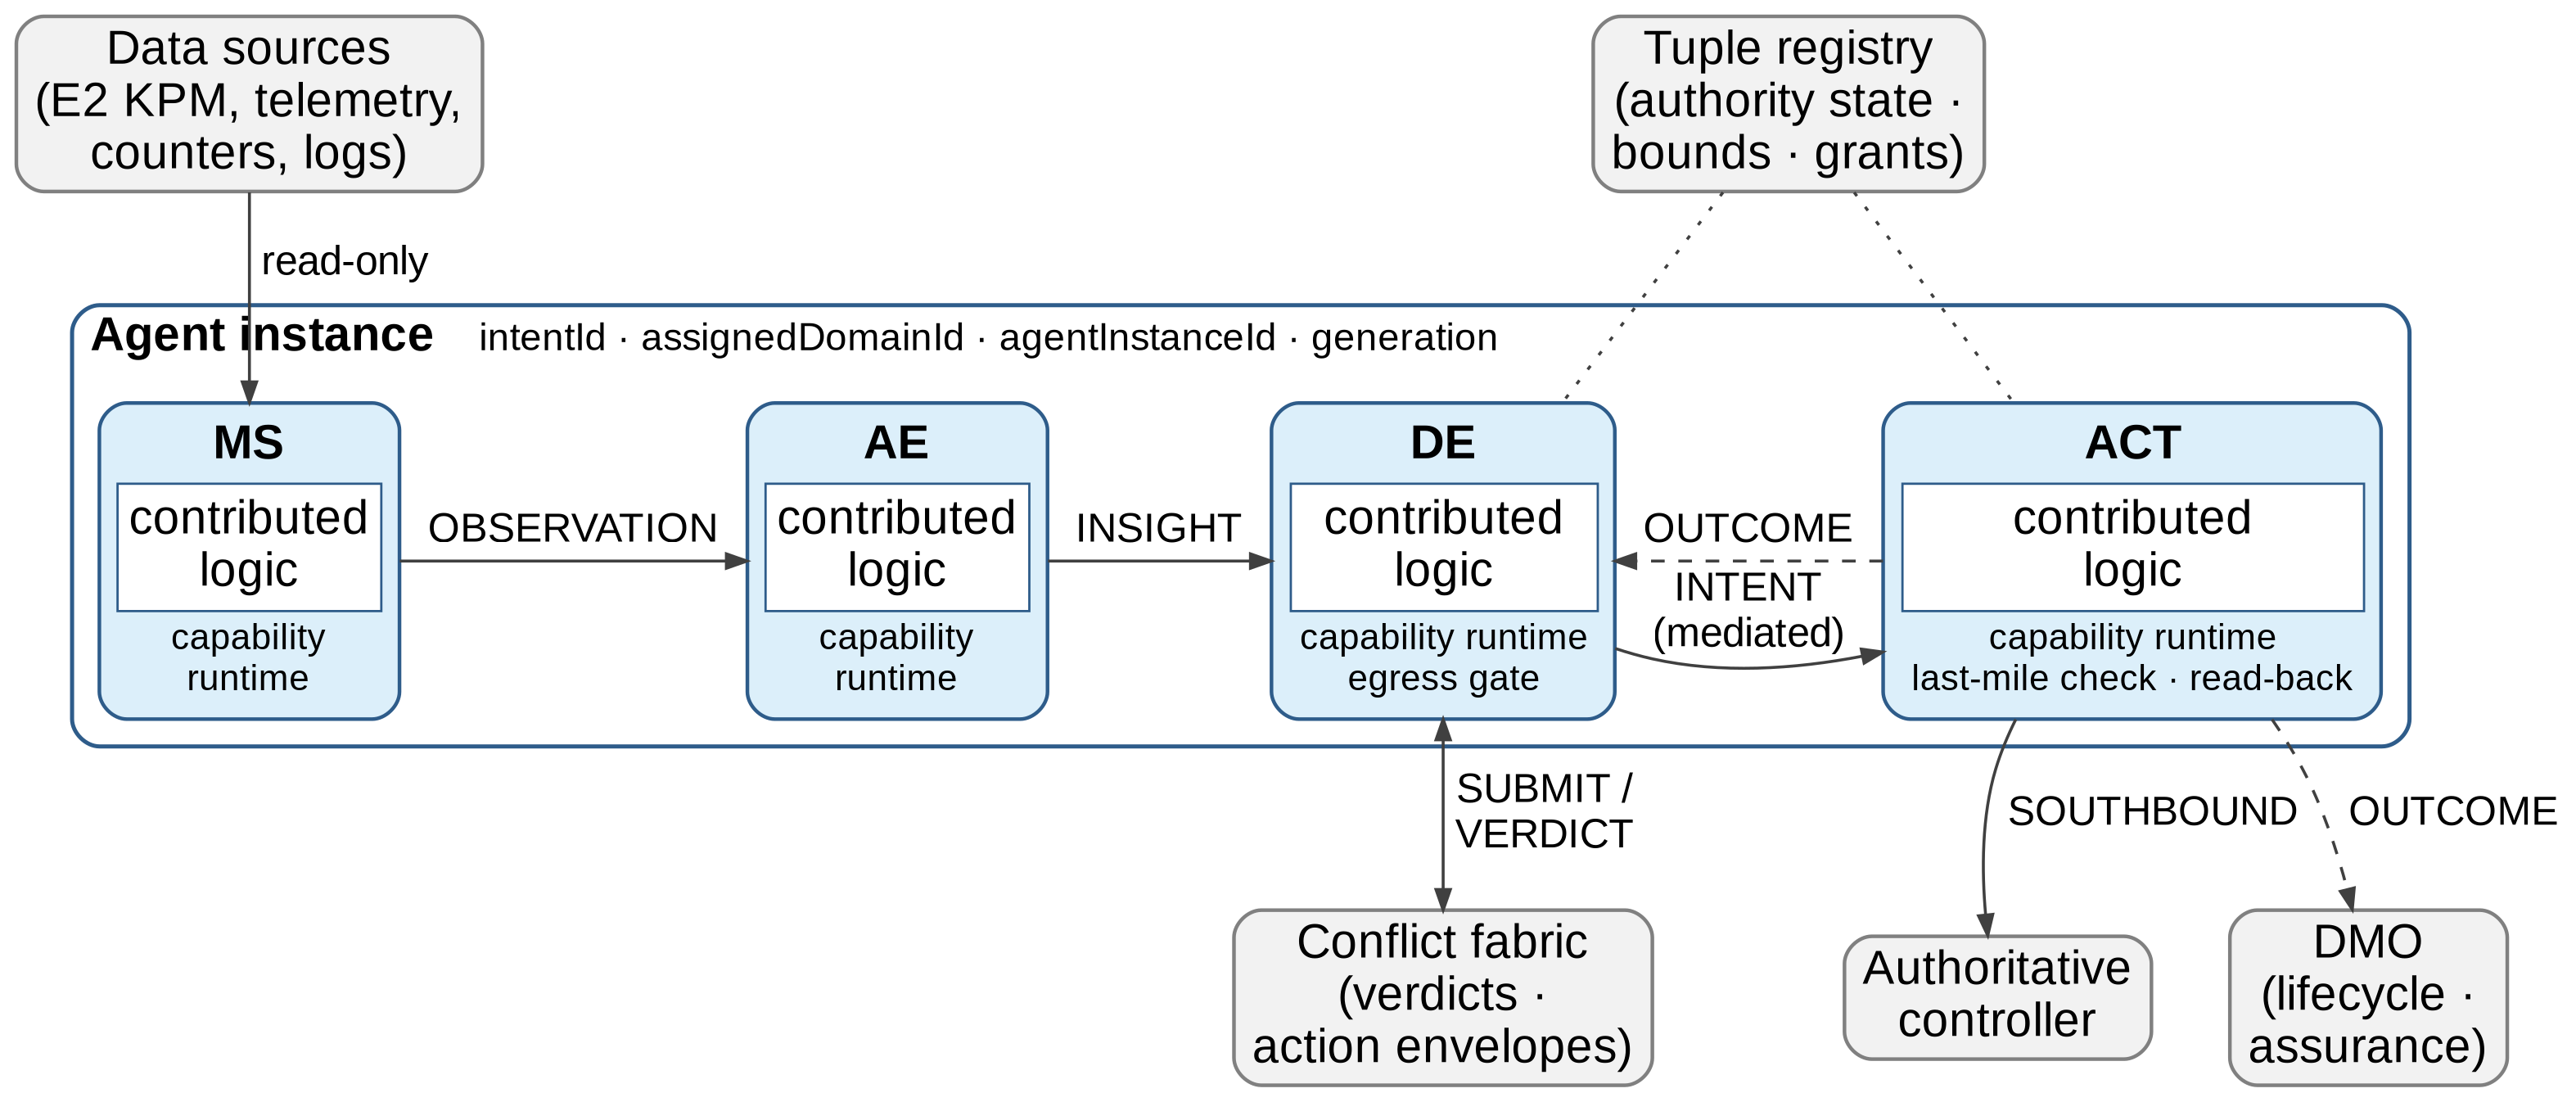
\includegraphics[width=\linewidth,height=0.45\textheight,keepaspectratio]{figures/image1.png}
\captionnum{3-1}
\caption{Anatomy of an agent instance}
\label{fig:3-1}
\end{figure}

\begin{wptable}{3-4}

\begin{longtable}[]{@{}
  >{\raggedright\arraybackslash}p{(\columnwidth - 8\tabcolsep) * \real{0.1312}}
  >{\raggedright\arraybackslash}p{(\columnwidth - 8\tabcolsep) * \real{0.2063}}
  >{\raggedright\arraybackslash}p{(\columnwidth - 8\tabcolsep) * \real{0.1937}}
  >{\raggedright\arraybackslash}p{(\columnwidth - 8\tabcolsep) * \real{0.2562}}
  >{\raggedright\arraybackslash}p{(\columnwidth - 8\tabcolsep) * \real{0.2126}}@{}}
\caption{The four capabilities}\tabularnewline
\toprule\noalign{}
\begin{minipage}[b]{\linewidth}\raggedright
\textbf{Capability}
\end{minipage} & \begin{minipage}[b]{\linewidth}\raggedright
\textbf{Consumes}
\end{minipage} & \begin{minipage}[b]{\linewidth}\raggedright
\textbf{Produces}
\end{minipage} & \begin{minipage}[b]{\linewidth}\raggedright
\textbf{Shall not produce}
\end{minipage} & \begin{minipage}[b]{\linewidth}\raggedright
\textbf{Typical placement}
\end{minipage} \\
\midrule\noalign{}
\endfirsthead
\toprule\noalign{}
\begin{minipage}[b]{\linewidth}\raggedright
\textbf{Capability}
\end{minipage} & \begin{minipage}[b]{\linewidth}\raggedright
\textbf{Consumes}
\end{minipage} & \begin{minipage}[b]{\linewidth}\raggedright
\textbf{Produces}
\end{minipage} & \begin{minipage}[b]{\linewidth}\raggedright
\textbf{Shall not produce}
\end{minipage} & \begin{minipage}[b]{\linewidth}\raggedright
\textbf{Typical placement}
\end{minipage} \\
\midrule\noalign{}
\endhead
\bottomrule\noalign{}
\endlastfoot
\textbf{MS} & Raw telemetry, events, logs and state from declared
sources, read-only & Observations, with coverage and data quality
signals & Scores, forecasts, classifications or confidence; any value
not measured & Device or edge, beside the data source \\
\textbf{AE} & Observations, or data products of the Data Continuum &
Insights, with model confidence, input quality and validity state &
Action identifiers, target configurations, parameter values to apply,
controller references & Edge, regional or central; principal consumer of
accelerators \\
\textbf{DE} & Insights (observations where the AE is none), objectives,
state, verdicts, outcomes & Intents, with structured rationale &
Controller-native commands; any intent that bypasses mediation & As the
loop\textquotesingle s latency class requires: DU/CU, Near-RT RIC,
regional or central \\
\textbf{ACT} & Mediated intents; state of the target & Controller
commands; outcomes & Decisions; any command outside the registered
action space & Beside the authoritative controller \\
\end{longtable}

\end{wptable}

\hypertarget{logical-flows-and-semantic-objects}{%
\subsubsection{Logical flows and semantic objects}\label{logical-flows-and-semantic-objects}}

Four logical flows connect the capabilities: OBSERVATION from MS to AE,
INSIGHT from AE to DE, INTENT from DE to ACT, and OUTCOME from ACT to DE
and to the DMO. Where an agent has no AE, OBSERVATION flows from MS to
DE. A logical flow is the semantic obligation between two capabilities
and is the same in every deployment. The binding that realizes it --- an
in-process call, a governed stream of the Data Continuum, an SMB topic
or a controller interface --- is selected per edge at realization
(Chapter 8) and changes neither the schema of the flow, nor its
validation, nor its audit.

Each flow carries one semantic object (Table 3-5). Some fields of each
object are computed by the capability runtime and some are supplied by
contributed logic. A field marked as platform-computed shall never be
accepted from contributed logic, and an object containing content
prohibited for its type is rejected at the binding boundary.

\begin{wptable}{3-5}

\begin{longtable}[]{@{}
  >{\raggedright\arraybackslash}p{(\columnwidth - 6\tabcolsep) * \real{0.1499}}
  >{\raggedright\arraybackslash}p{(\columnwidth - 6\tabcolsep) * \real{0.1499}}
  >{\raggedright\arraybackslash}p{(\columnwidth - 6\tabcolsep) * \real{0.4312}}
  >{\raggedright\arraybackslash}p{(\columnwidth - 6\tabcolsep) * \real{0.2689}}@{}}
\caption{Semantic objects of the logical flows}\tabularnewline
\toprule\noalign{}
\begin{minipage}[b]{\linewidth}\raggedright
\textbf{Object}
\end{minipage} & \begin{minipage}[b]{\linewidth}\raggedright
\textbf{Flow}
\end{minipage} & \begin{minipage}[b]{\linewidth}\raggedright
\textbf{Mandatory content (P: platform-computed)}
\end{minipage} & \begin{minipage}[b]{\linewidth}\raggedright
\textbf{Prohibited content}
\end{minipage} \\
\midrule\noalign{}
\endfirsthead
\toprule\noalign{}
\begin{minipage}[b]{\linewidth}\raggedright
\textbf{Object}
\end{minipage} & \begin{minipage}[b]{\linewidth}\raggedright
\textbf{Flow}
\end{minipage} & \begin{minipage}[b]{\linewidth}\raggedright
\textbf{Mandatory content (P: platform-computed)}
\end{minipage} & \begin{minipage}[b]{\linewidth}\raggedright
\textbf{Prohibited content}
\end{minipage} \\
\midrule\noalign{}
\endhead
\bottomrule\noalign{}
\endlastfoot
\textbf{Observation} & MS → AE; MS → DE where the AE is none &
Measurement records: object, metric, value, unit, event time. Data
quality signals. scope\_\allowbreak{}coverage (P): cardinality of the
declared scope, cardinality observed in the interval, enumerated
unobserved members. Stale marker (P). & Model outputs, scores,
forecasts, classifications, confidence fields; values not measured \\
\textbf{Insight} & AE → DE & insight\_\allowbreak{}type, one of the
declared types; payload; model\_\allowbreak{}confidence.\allowbreak{}
input\_\allowbreak{}quality (P): minimum input coverage, maximum input
staleness, identifiers of the contributing envelopes,
degraded\_\allowbreak{}input.\allowbreak{} validity\_\allowbreak{}state
(P): in\_\allowbreak{}envelope or
out\_\allowbreak{}of\_\allowbreak{}envelope.\allowbreak{} Model
identifier and version (P). & Action identifiers, target configurations,
parameter values to be applied, controller references \\
\textbf{Intent} & DE → ACT & Action type; targets; parameters; validity
window; urgency within the registered band; decision confidence;
rationale: insights consumed, constraints applied, objectives, reason
code. Mediation reference (P): verdict, grant or policy evaluation
record. correlationId (P). & Controller-native command fields; rationale
in free text only \\
\textbf{Outcome} & ACT → DE and DMO & Outcome:
ACKNOWLEDGED\_\allowbreak{}VERIFIED,
ACKNOWLEDGED\_\allowbreak{}UNVERIFIED, REJECTED or UNRESOLVED;
provisional or final; applied configuration where known; read-back
evidence; timing; reason code; correlationId. Every field is
platform-computed. & --- \\
\end{longtable}

\end{wptable}

Every message on every binding carries the message envelope of Table 3-6
in addition to its semantic object. A message that lacks a mandatory
envelope structure is rejected at the binding boundary; it is not logged
and forwarded. The envelope is specified field by field in Chapter 8.

\begin{wptable}{3-6}

\begin{longtable}[]{@{}
  >{\raggedright\arraybackslash}p{(\columnwidth - 4\tabcolsep) * \real{0.1499}}
  >{\raggedright\arraybackslash}p{(\columnwidth - 4\tabcolsep) * \real{0.6000}}
  >{\raggedright\arraybackslash}p{(\columnwidth - 4\tabcolsep) * \real{0.2501}}@{}}
\caption{The message envelope}\tabularnewline
\toprule\noalign{}
\begin{minipage}[b]{\linewidth}\raggedright
\textbf{Structure}
\end{minipage} & \begin{minipage}[b]{\linewidth}\raggedright
\textbf{Content}
\end{minipage} & \begin{minipage}[b]{\linewidth}\raggedright
\textbf{Populated by}
\end{minipage} \\
\midrule\noalign{}
\endfirsthead
\toprule\noalign{}
\begin{minipage}[b]{\linewidth}\raggedright
\textbf{Structure}
\end{minipage} & \begin{minipage}[b]{\linewidth}\raggedright
\textbf{Content}
\end{minipage} & \begin{minipage}[b]{\linewidth}\raggedright
\textbf{Populated by}
\end{minipage} \\
\midrule\noalign{}
\endhead
\bottomrule\noalign{}
\endlastfoot
\textbf{time} & event\_\allowbreak{}time at the source;
ingest\_\allowbreak{}time at the collecting runtime & Runtime;
event\_\allowbreak{}time from the source where available \\
\textbf{scope} & Domain; scope-tag values for region, site, slice,
tenant and technology, pseudonymized across trust boundaries & Runtime,
from the granted scope \\
\textbf{provenance} & Producer descriptor\_\allowbreak{}id and version;
agentInstanceId; globalAgentId and delegationId where applicable; model
identifier and version, feature-set version and policy version where
applicable & Runtime, from the registry \\
\textbf{control} & messageId; validity window; priority; required
acknowledgements; rollback handle; correlationId & Runtime; priority
from the registered band \\
\textbf{generation} & Generation of the producing instance & Runtime,
from the registry \\
\end{longtable}

\end{wptable}

Beyond the four flows, an agent takes part in control exchanges that are
not flows between its own capabilities: SUBMIT, VERDICT and NOTIFY
between the DE and the conflict fabric (Chapter 10); lifecycle, health
and conformance events between each capability runtime and the DMO
(Chapter 9); and, for a global agent, the delegation operations its ACT
issues towards DMOs (Chapter 8).

\hypertarget{from-tuple-to-agent}{%
\subsubsection{From tuple to agent}\label{from-tuple-to-agent}}

A tuple is a structure; an agent is a tuple given something to achieve
and the authority to pursue it. An agent comprises:

\begin{itemize}
\tightlist
\item
  a tuple, with a capability mode declared for each of the four
  capabilities;
\item
  one or more objectives, declared in the descriptor as templates over
  catalog KPIs and bound to target values once, when the agent is
  instantiated;
\item
  scope: what the agent may observe and what it may change;
\item
  authority: declared in the descriptor, bounded by the delegation where
  the agent realizes one, granted at admission and held in the registry
  as an authority state;
\item
  declared behavior: a failure policy for each capability, stability
  controls on each action, and a conflict-resolution policy;
\item
  identity: the identity and version of its descriptor, and the identity
  and generation of the instance.
\end{itemize}

The agent descriptor defines an agent type. An agent instance realizes
the descriptor in one domain, or at the IDMO for a global agent. Two
instantiations of the same descriptor create two instances, isolated
from each other as stated in Section 3.1.3.

\hypertarget{invariants}{%
\subsubsection{Invariants}\label{invariants}}

The invariants of Table 3-7 hold for every agent, irrespective of its
declaration, its conformance class and its authority state. They are not
fields of the descriptor and cannot be relaxed by declaration, by
agreement or by configuration. Each is carried by a requirement of the
capability, interconnection, lifecycle or conflict chapters and is
enforced at the point stated.

\begin{wptable}{3-7}

\begin{longtable}[]{@{}
  >{\raggedright\arraybackslash}p{(\columnwidth - 4\tabcolsep) * \real{0.1000}}
  >{\raggedright\arraybackslash}p{(\columnwidth - 4\tabcolsep) * \real{0.5875}}
  >{\raggedright\arraybackslash}p{(\columnwidth - 4\tabcolsep) * \real{0.3125}}@{}}
\caption{Invariants}\tabularnewline
\toprule\noalign{}
\begin{minipage}[b]{\linewidth}\raggedright
\textbf{ID}
\end{minipage} & \begin{minipage}[b]{\linewidth}\raggedright
\textbf{Invariant}
\end{minipage} & \begin{minipage}[b]{\linewidth}\raggedright
\textbf{Enforced at}
\end{minipage} \\
\midrule\noalign{}
\endfirsthead
\toprule\noalign{}
\begin{minipage}[b]{\linewidth}\raggedright
\textbf{ID}
\end{minipage} & \begin{minipage}[b]{\linewidth}\raggedright
\textbf{Invariant}
\end{minipage} & \begin{minipage}[b]{\linewidth}\raggedright
\textbf{Enforced at}
\end{minipage} \\
\midrule\noalign{}
\endhead
\bottomrule\noalign{}
\endlastfoot
\textbf{INV-1} & The MS produces evidence, never conclusions. &
Admission (contract shape); binding boundary \\
\textbf{INV-2} & The MS never presents as measured a value it did not
measure; gaps are published as gaps. & MS runtime \\
\textbf{INV-3} & The AE produces insight, never action. & Admission;
binding boundary \\
\textbf{INV-4} & A fallback heuristic is used only if it was declared. &
Admission; AE runtime \\
\textbf{INV-5} & The DE emits intent, never controller-native commands.
& Admission; binding boundary \\
\textbf{INV-6} & A DE cannot approve its own intents. & DE post-gate;
activation gate \\
\textbf{INV-7} & Where declared failure behavior is absent or ambiguous
at runtime, the DE emits no intent. & DE runtime \\
\textbf{INV-8} & The ACT translates intent; it does not decide. &
Admission (deterministic translation); ACT runtime \\
\textbf{INV-9} & An acknowledgement is never proof of change. & ACT
runtime (verification) \\
\textbf{INV-10} & A timeout is an unresolved transaction, not permission
to retry. & ACT runtime (retry matrix) \\
\textbf{INV-11} & A message missing a mandatory structure is rejected,
not forwarded. & Every binding boundary \\
\textbf{INV-12} & A message of an older generation than the
receiver\textquotesingle s binding record is discarded. & Every
receiving runtime \\
\textbf{INV-13} & A DMO rejects or escalates any instruction that would
violate a local safety or regulatory constraint. & DMO, on every
delegation, update and intent \\
\textbf{INV-14} & A platform-computed field is never accepted from
contributed logic. & Capability runtimes \\
\textbf{INV-15} & Authority is held in the registry; no message confers
authority that the registry does not hold, and a request beyond
registered scope is a violation, not a conflict. & Conflict fabric; DE
post-gate; ACT last-mile check \\
\end{longtable}

\end{wptable}

\hypertarget{capability-modes}{%
\subsubsection{Capability modes}\label{capability-modes}}

Each capability is declared in exactly one of four modes (Table 3-8). A
mode states who performs the capability for the agent. It does not state
where the capability runs, which is declared in the physical deployment
(Section 3.5.12), nor with what authority, which is held as an authority
state (Section 3.4.7).

\begin{wptable}{3-8}

\begin{longtable}[]{@{}
  >{\raggedright\arraybackslash}p{(\columnwidth - 6\tabcolsep) * \real{0.1250}}
  >{\raggedright\arraybackslash}p{(\columnwidth - 6\tabcolsep) * \real{0.3625}}
  >{\raggedright\arraybackslash}p{(\columnwidth - 6\tabcolsep) * \real{0.2625}}
  >{\raggedright\arraybackslash}p{(\columnwidth - 6\tabcolsep) * \real{0.2499}}@{}}
\caption{Capability modes}\tabularnewline
\toprule\noalign{}
\begin{minipage}[b]{\linewidth}\raggedright
\textbf{Mode}
\end{minipage} & \begin{minipage}[b]{\linewidth}\raggedright
\textbf{Meaning}
\end{minipage} & \begin{minipage}[b]{\linewidth}\raggedright
\textbf{Declared with}
\end{minipage} & \begin{minipage}[b]{\linewidth}\raggedright
\textbf{Admission check}
\end{minipage} \\
\midrule\noalign{}
\endfirsthead
\toprule\noalign{}
\begin{minipage}[b]{\linewidth}\raggedright
\textbf{Mode}
\end{minipage} & \begin{minipage}[b]{\linewidth}\raggedright
\textbf{Meaning}
\end{minipage} & \begin{minipage}[b]{\linewidth}\raggedright
\textbf{Declared with}
\end{minipage} & \begin{minipage}[b]{\linewidth}\raggedright
\textbf{Admission check}
\end{minipage} \\
\midrule\noalign{}
\endhead
\bottomrule\noalign{}
\endlastfoot
\textbf{full} & The agent\textquotesingle s own contributed logic
performs the capability within the agent\textquotesingle s scope. & The
capability\textquotesingle s section in functions & Function section
complete and valid \\
\textbf{partial} & The agent\textquotesingle s own logic performs an
enumerated subset --- for the MS a subset of the observation scope, for
the AE a subset of insight types, for the DE a restricted decision
space, for the ACT a subset of the action space. The complement is not
performed unless a delegation covers it. &
capability\_\allowbreak{}subsets.\allowbreak{}\textless cap\textgreater;
optionally a delegation covering the complement & Subset non-empty and
contained in the declared scope or space; an unenumerated partial
capability is rejected \\
\textbf{delegated} & A named provider performs the capability: another
agent, a platform service or a reused capability, bound through a pinned
contract. &
capability\_\allowbreak{}delegations.\allowbreak{}\textless cap\textgreater{}
& Provider resolvable; provider scope covers the
consumer\textquotesingle s; interface profile pinned; provider version
within range; provider\textquotesingle s declared latency and freshness
within the SLA assumptions \\
\textbf{none} & The capability is absent. & --- & Composition class
derivable (Table 3-9) \\
\end{longtable}

\end{wptable}

Two further rules complete the modes. First, an agent whose DE is
present and whose AE is none consumes observations directly; its DE
runtime then computes the quality of its input from the observations
consumed, exactly as an AE runtime would, so that degraded evidence is
detected whatever the composition. Second, a delegation crosses a domain
boundary only for the AE, whose insight may be consumed across domains
as a data product or through an exposed contract, and for the DE of a
local agent whose provider is the agent's own global agent. MS and ACT
delegations remain within the domain: raw telemetry does not leave its
domain, and a domain's controllers are reached only through that
domain's actuators.

\hypertarget{composition-classes}{%
\subsubsection{Composition classes}\label{composition-classes}}

The platform derives a composition class from the four capability modes
(Table 3-9). The class is not declared in the descriptor. It determines
the highest authority state the agent can hold and the way the agent is
registered. Any combination of modes that fits none of the classes is
invalid.

\begin{wptable}{3-9}

\begin{longtable}[]{@{}
  >{\raggedright\arraybackslash}p{(\columnwidth - 6\tabcolsep) * \real{0.1813}}
  >{\raggedright\arraybackslash}p{(\columnwidth - 6\tabcolsep) * \real{0.3125}}
  >{\raggedright\arraybackslash}p{(\columnwidth - 6\tabcolsep) * \real{0.2000}}
  >{\raggedright\arraybackslash}p{(\columnwidth - 6\tabcolsep) * \real{0.3063}}@{}}
\caption{Composition classes}\tabularnewline
\toprule\noalign{}
\begin{minipage}[b]{\linewidth}\raggedright
\textbf{Class}
\end{minipage} & \begin{minipage}[b]{\linewidth}\raggedright
\textbf{Condition on capability modes}
\end{minipage} & \begin{minipage}[b]{\linewidth}\raggedright
\textbf{Authority ceiling}
\end{minipage} & \begin{minipage}[b]{\linewidth}\raggedright
\textbf{Registration}
\end{minipage} \\
\midrule\noalign{}
\endfirsthead
\toprule\noalign{}
\begin{minipage}[b]{\linewidth}\raggedright
\textbf{Class}
\end{minipage} & \begin{minipage}[b]{\linewidth}\raggedright
\textbf{Condition on capability modes}
\end{minipage} & \begin{minipage}[b]{\linewidth}\raggedright
\textbf{Authority ceiling}
\end{minipage} & \begin{minipage}[b]{\linewidth}\raggedright
\textbf{Registration}
\end{minipage} \\
\midrule\noalign{}
\endhead
\bottomrule\noalign{}
\endlastfoot
\textbf{closed\_\allowbreak{}loop} & DE and ACT not none; MS or AE not
none & closed\_\allowbreak{}loop\_\allowbreak{}full & Closed-loop agent;
control parameters and objective KPIs registered with the conflict
fabric \\
\textbf{open\_\allowbreak{}loop} & DE not none; ACT none; MS or AE not
none & advisory & Advisory agent; intents published as recommendations;
no actuation path \\
\textbf{analytics} & AE full or partial; DE and ACT none &
monitoring\_\allowbreak{}only & Insight provider; may expose insight
contracts and serve as a delegated AE \\
\textbf{observation} & MS full or partial; AE, DE and ACT none &
monitoring\_\allowbreak{}only & Observation provider; may serve as a
delegated MS \\
\textbf{actuation\_\allowbreak{}service} & ACT full or partial; MS, AE
and DE none & closed\_\allowbreak{}loop\_\allowbreak{}full, exercised
only on the intents of delegating agents & Actuation provider; executes
only the mediated intents of agents that delegate their ACT to it; every
outcome is attributed to the delegating agent \\
\end{longtable}

\end{wptable}

A global agent is of class closed\_\allowbreak{}loop,
open\_\allowbreak{}loop or analytics. Its ACT acts on the management
hierarchy --- it creates, updates, approves, suspends and terminates
delegations and issues intents towards DMOs --- and never on
infrastructure.

\hypertarget{taxonomy}{%
\subsection{Taxonomy}\label{taxonomy}}

\hypertarget{dimensions-of-classification}{%
\subsubsection{Dimensions of classification}\label{dimensions-of-classification}}

Agents and contributions are classified along the ten dimensions of
Table 3-10. Each dimension is either declared or derived. A derived
dimension cannot be declared, and a declared dimension is checked
against what the rest of the descriptor supports. The classification of
every agent instance is recorded in the registry and reported in
assurance.

\begin{wptable}{3-10}

\begin{longtable}[]{@{}
  >{\raggedright\arraybackslash}p{(\columnwidth - 6\tabcolsep) * \real{0.1625}}
  >{\raggedright\arraybackslash}p{(\columnwidth - 6\tabcolsep) * \real{0.3375}}
  >{\raggedright\arraybackslash}p{(\columnwidth - 6\tabcolsep) * \real{0.1875}}
  >{\raggedright\arraybackslash}p{(\columnwidth - 6\tabcolsep) * \real{0.3125}}@{}}
\caption{Dimensions of classification}\tabularnewline
\toprule\noalign{}
\begin{minipage}[b]{\linewidth}\raggedright
\textbf{Dimension}
\end{minipage} & \begin{minipage}[b]{\linewidth}\raggedright
\textbf{Values}
\end{minipage} & \begin{minipage}[b]{\linewidth}\raggedright
\textbf{Declared or derived}
\end{minipage} & \begin{minipage}[b]{\linewidth}\raggedright
\textbf{Determines}
\end{minipage} \\
\midrule\noalign{}
\endfirsthead
\toprule\noalign{}
\begin{minipage}[b]{\linewidth}\raggedright
\textbf{Dimension}
\end{minipage} & \begin{minipage}[b]{\linewidth}\raggedright
\textbf{Values}
\end{minipage} & \begin{minipage}[b]{\linewidth}\raggedright
\textbf{Declared or derived}
\end{minipage} & \begin{minipage}[b]{\linewidth}\raggedright
\textbf{Determines}
\end{minipage} \\
\midrule\noalign{}
\endhead
\bottomrule\noalign{}
\endlastfoot
\textbf{Composition class} & closed\_\allowbreak{}loop,
open\_\allowbreak{}loop, analytics, observation,
actuation\_\allowbreak{}service & Derived from the capability modes &
Authority ceiling; registration with the conflict fabric \\
\textbf{Scope class} & local, global, hybrid & Derived from the
descriptor kind and delegations & Owner of the registry entry;
descriptor level; latency classes available \\
\textbf{Latency class} & real\_\allowbreak{}time,
near\_\allowbreak{}real\_\allowbreak{}time,
non\_\allowbreak{}real\_\allowbreak{}time, offline & Declared; effective
class derived at admission & Loop budget; deadlines; fast-path
conditions \\
\textbf{Operating mode} & continuous, event\_\allowbreak{}driven,
scheduled, on\_\allowbreak{}demand & Declared & What starts a cycle;
triggers of the capability functions \\
\textbf{Domain} & core, oran, ntn, transport, non3gpp\_\allowbreak{}ran,
aiml, vertical\_\allowbreak{}app, digital\_\allowbreak{}twin; idmo for
global agents & Declared & Owning DMO; controller bindings; catalog
entries available \\
\textbf{Contribution class} & role\_\allowbreak{}implementation,
platform\_\allowbreak{}service, reused\_\allowbreak{}capability,
supporting\_\allowbreak{}application & Declared at catalog registration
& Contract applied: capability contracts or service contract \\
\textbf{Conformance class} & normative, extension & Derived from
extension fields and types & Entry authority; promotion path \\
\textbf{Technique class} & deterministic, optimization,
classical\_\allowbreak{}ml, reinforcement\_\allowbreak{}learning,
generative, digital\_\allowbreak{}twin, hybrid; per capability &
Declared & Admissibility and its conditions (Table 3-11) \\
\textbf{Realization pattern} & full\_\allowbreak{}tuple,
partial\_\allowbreak{}tuple, reused\_\allowbreak{}services,
hierarchical\_\allowbreak{}local\_\allowbreak{}tuple,
advisory\_\allowbreak{}tuple & Selected by the DMO at realization &
Capabilities deployed, reused or delegated \\
\textbf{Authority state} & The seven states of Table 3-12 & Held in the
registry; changes at runtime & What the instance may do at a given
moment \\
\end{longtable}

\end{wptable}

The domain digital\_\allowbreak{}twin is the Digital Twin domain of the
architecture, and agents are placed in it as in any other domain. It is
distinct from the technique class digital\_\allowbreak{}twin, by which
an agent of any domain evaluates through simulation. An agent of the
digital\_\allowbreak{}twin domain observes and manages the twins and the
platform that hosts them as managed objects; what a twin simulates is
not a measurement of the network, whatever the domain of the agent that
uses it (Table 3-11).

\hypertarget{scope-classes-local-global-and-hybrid-agents}{%
\subsubsection{Scope classes: local, global and hybrid agents}\label{scope-classes-local-global-and-hybrid-agents}}

A local agent is described by a LocalAINativeAgent descriptor and owned
by one DMO. Its capabilities are realized within one domain, or
delegated within it, with the two cross-domain exceptions of Section
3.3.5. It closes its loop locally, in whichever latency class its
assembled path can sustain, and acts on infrastructure through its
domain's controllers (Figure 3-2 (a)).

A global agent is described by a GlobalAINativeAgent descriptor and
owned by the IDMO. Its MS observes domain summaries, the global
topology, global service and KPI state and the health of the DMOs; its
AE correlates across domains, analyzes impact and predicts end-to-end
behavior; its DE decides global strategy and the division of
responsibility between domains; its ACT acts on the management hierarchy
through delegation operations. A global agent holds the non-real-time or
the offline class only (Figure 3-2 (b)). The DMOs fulfill its
delegations either with local agents or with conventionally managed
domain services.

A hybrid agent --- the cooperative form --- is a global agent together
with the local agents that realize its delegations, operating as one
logical agent under one globalAgentId (Figure 3-2 (c)). The global tuple
sets objectives and authority envelopes on the non-real-time loop; each
local tuple acts within its authority envelope, in its own latency
class. The local agents of a hybrid exchange nothing with each other
directly. Coordination between domains passes through delegation
channels, through cross-domain bindings provisioned by the IDMO and
through the conflict fabric, and evidence flows upward as features,
summaries and events, never as raw telemetry. Every message of a local
agent that realizes a delegation carries the globalAgentId and the
delegationId in its provenance.

An objective spanning several domains is served either by independent
local agents, one per domain, coordinated only by the decomposition of
the objective and by the conflict fabric, or by a hybrid agent. A hybrid
agent is required where the division of responsibility between domains
must change during the life of the objective without a new order.
Otherwise independent local agents suffice, and a change in the division
of responsibility requires a new order.

\begin{figure}[htbp]
\centering
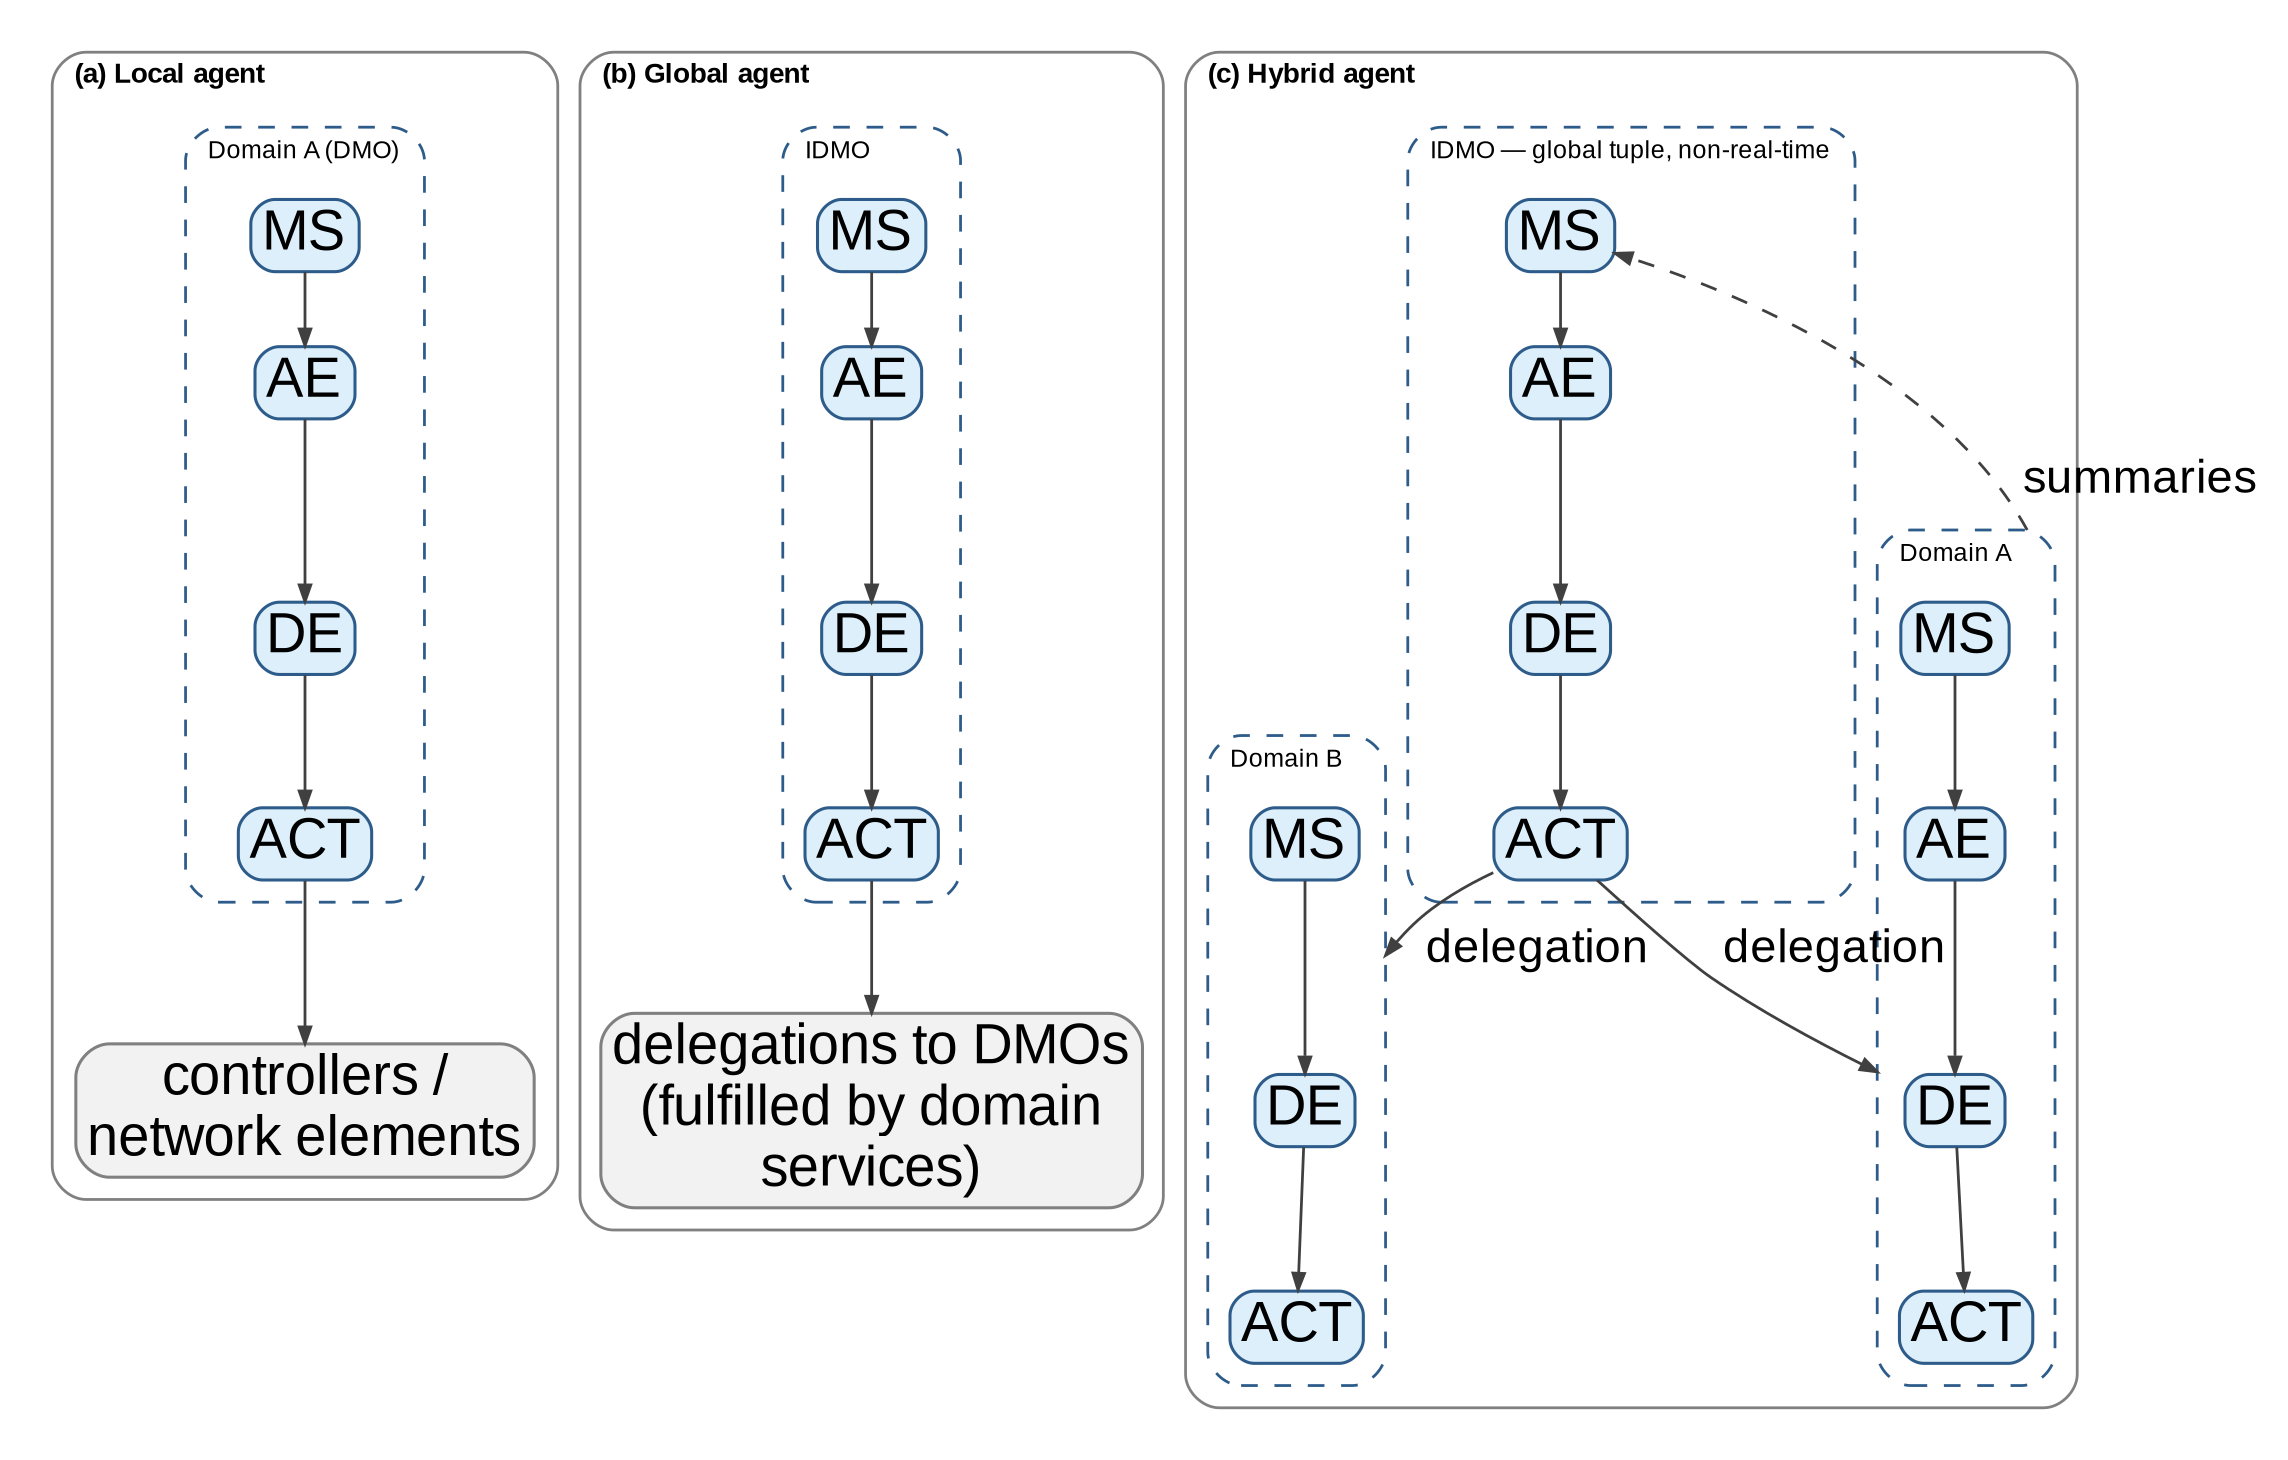
\includegraphics[width=\linewidth,height=0.45\textheight,keepaspectratio]{figures/image2.png}
\captionnum{3-2}
\caption{Local, global and hybrid agents}
\label{fig:3-2}
\end{figure}

\hypertarget{realization-patterns}{%
\subsubsection{Realization patterns}\label{realization-patterns}}

The DMO realizes a local agent according to one of five patterns, chosen
from the descriptor's capability modes, the delegation where the agent
realizes one, and the functions available in the domain's catalog:

\begin{itemize}
\tightlist
\item
  \emph{full tuple} --- MS, AE, DE and ACT deployed locally, for fast
  autonomous operation of the domain;
\item
  \emph{partial tuple} --- MS and ACT deployed locally, with AE and DE
  delegated to the agent's global agent, where global intelligence
  suffices and only local enforcement is needed;
\item
  \emph{reused services} --- an existing monitoring stack or controller
  bound as the provider of a delegated MS or ACT, with a new AE and DE
  deployed;
\item
  \emph{hierarchical local tuple} --- several MS instances, each
  observing part of a large or distributed domain, feeding one
  domain-level AE and DE;
\item
  \emph{advisory tuple} --- MS, AE and DE deployed with the agent held
  in the advisory authority state, so that actuation requires approval.
\end{itemize}

The descriptor constrains the choice of pattern through its capability
modes and its permitted binding classes, but does not name a pattern.
The pattern selected is recorded in the registry and in the resolved
configuration.

\hypertarget{contribution-classes}{%
\subsubsection{Contribution classes}\label{contribution-classes}}

Every partner contribution enters the platform as exactly one of four
classes, declared when it is registered in the catalog:

\begin{itemize}
\tightlist
\item
  \emph{role implementation} --- supplies the behavior of one or more
  capabilities of an agent, is described by an agent descriptor and is
  held to the full capability contracts. This is the ordinary case: for
  example the WP5 applications App-01 to App-04, App-06, App-07, App-09
  and App-12 to App-15, and the WP4 algorithms DPIR and RF-PLRE;
\item
  \emph{platform service} --- supplies a capability that the platform
  itself consumes and holds no role in any agent; it is held to its
  service contract. The conflict management service (App-10) and the
  trust modeling service (App-11) are platform services: the former is
  bound at the activation gate as the mediation endpoint and never
  mediates itself, and the latter enters at admission and registration
  and never on the per-decision path;
\item
  \emph{reused capability} --- an existing service bound as a provider
  rather than deployed, such as a monitoring stack, a model registry or
  a domain controller;
\item
  \emph{supporting application} --- operates alongside agents without
  holding a role in one, such as the XR application (App-05) or semantic
  domain switching offered as a service-level function (App-08).
\end{itemize}

Only role implementations are described by agent descriptors. The other
three classes are registered in the catalog with their service contracts
(Section 3.6) and may appear in a descriptor only as providers of
delegated capabilities or as endpoints of bindings.

\hypertarget{conformance-classes-and-the-extension-path}{%
\subsubsection{Conformance classes and the extension path}\label{conformance-classes-and-the-extension-path}}

A descriptor whose every declaration uses the normative schema and
catalog types is of normative conformance. A descriptor that contains an
extension field or references an extension type (Section 3.5.17) is of
extension conformance. The class is derived by the platform.

An extension agent enters at the advisory authority state. Its
containment is identical to that of a normative agent: the same egress
gate, the same mediation, the same stability enforcement, the same
rationale requirement and the same last-mile check apply. Freedom
applies to its algorithm, not to its guardrails. Sustained conformant
operation under evaluation is the route to promotion --- from advisory
to closed\_\allowbreak{}loop\_\allowbreak{}reduced and then to
closed\_\allowbreak{}loop\_\allowbreak{}full, under the criteria of
Chapter 9 --- and to the adoption of its extension types into the
catalog, after which the descriptor is republished at normative
conformance.

\hypertarget{technique-classes-and-admissibility}{%
\subsubsection{Technique classes and admissibility}\label{technique-classes-and-admissibility}}

Contributed logic declares its technique class per capability. The
technique changes no contract; it determines whether the logic is
admissible in a capability at all, and under which conditions (Table
3-11). A hybrid technique is subject to the conditions of every
technique it combines.

\begin{wptable}{3-11}

\begin{longtable}[]{@{}
  >{\raggedright\arraybackslash}p{(\columnwidth - 8\tabcolsep) * \real{0.1625}}
  >{\raggedright\arraybackslash}p{(\columnwidth - 8\tabcolsep) * \real{0.2094}}
  >{\raggedright\arraybackslash}p{(\columnwidth - 8\tabcolsep) * \real{0.2094}}
  >{\raggedright\arraybackslash}p{(\columnwidth - 8\tabcolsep) * \real{0.2094}}
  >{\raggedright\arraybackslash}p{(\columnwidth - 8\tabcolsep) * \real{0.2094}}@{}}
\caption{Admissibility of technique classes by
capability}\tabularnewline
\toprule\noalign{}
\begin{minipage}[b]{\linewidth}\raggedright
\textbf{Technique class}
\end{minipage} & \begin{minipage}[b]{\linewidth}\raggedright
\textbf{MS}
\end{minipage} & \begin{minipage}[b]{\linewidth}\raggedright
\textbf{AE}
\end{minipage} & \begin{minipage}[b]{\linewidth}\raggedright
\textbf{DE}
\end{minipage} & \begin{minipage}[b]{\linewidth}\raggedright
\textbf{ACT}
\end{minipage} \\
\midrule\noalign{}
\endfirsthead
\toprule\noalign{}
\begin{minipage}[b]{\linewidth}\raggedright
\textbf{Technique class}
\end{minipage} & \begin{minipage}[b]{\linewidth}\raggedright
\textbf{MS}
\end{minipage} & \begin{minipage}[b]{\linewidth}\raggedright
\textbf{AE}
\end{minipage} & \begin{minipage}[b]{\linewidth}\raggedright
\textbf{DE}
\end{minipage} & \begin{minipage}[b]{\linewidth}\raggedright
\textbf{ACT}
\end{minipage} \\
\midrule\noalign{}
\endhead
\bottomrule\noalign{}
\endlastfoot
\textbf{deterministic (rules, thresholds, state machines)} & Admissible
& Admissible & Admissible & Admissible; the default for translation \\
\textbf{optimization (solvers, bounded heuristics)} & Admissible for
acquisition control, such as adaptive sampling & Admissible &
Admissible; solutions are checked against the action space like any
proposal & Admissible only with deterministic execution: fixed seed and
bounded run time \\
\textbf{classical\_\allowbreak{}ml (supervised, unsupervised,
statistical)} & Admissible for acquisition functions only; never for
values presented as measured & Admissible with pinned model identity,
machine-evaluable validity conditions and drift signals & Admissible &
Not admissible \\
\textbf{reinforcement\_\allowbreak{}learning} & Not admissible &
Admissible as a predictor, under the AE conditions & Admissible;
exploration only through ordinary intents, subject to every bound;
weight updates follow the adaptation rule & Not admissible \\
\textbf{generative (based on language models, including tool use and
multi-step planning)} & Admissible as a query or observability
interface; output traceable to collected data and never presented as
measurement & Admissible with declared uncertainty and machine-evaluable
validity conditions & Admissible with output confined to the registered
action space; entry at advisory; declared read-only tools only & Not
admissible \\
\textbf{digital\_\allowbreak{}twin (simulation-based evaluation)} & Not
admissible: simulated values are not measurements & Admissible; insights
labeled as simulated & Admissible as evaluation within the decision;
twin validation confers no authority & Not admissible \\
\end{longtable}

\end{wptable}

Adaptation during operation is declared in the model hooks (Section
3.5.15). Adaptation that changes model weights produces a new model
identity and takes effect only through a generation-controlled update
performed by the DMO (Chapter 9); an agent never replaces its own model.
Adaptation that accumulates context without changing weights, as in
agents based on language models with episodic memory, is declared with a
bound on the retained context and the condition on which the context is
reset, and the agent's validity conditions and drift signals apply to it
unchanged.

\hypertarget{authority-ceilings-and-authority-states}{%
\subsubsection{Authority ceilings and authority states}\label{authority-ceilings-and-authority-states}}

The capabilities realized for an agent are those its descriptor
declares, and the composition class they form (Table 3-9) sets the first
of its authority ceilings; no service request selects them. A domain in
which no agent is instantiated runs without one, so an end-to-end
service may span agent-managed and conventionally managed domains
(Section 3.10).

The authority ceiling of an instance is the lowest of four ceilings:
that of its composition class, that permitted by the authority mode its
descriptor declares, that set by the interpretability of its decision
logic, and, for extension conformance until promotion, advisory.
Ceilings are ordered monitoring\_\allowbreak{}only, advisory,
closed\_\allowbreak{}loop\_\allowbreak{}reduced and
closed\_\allowbreak{}loop\_\allowbreak{}full, from lowest to highest.
The authority mode auto\_\allowbreak{}execute permits
closed\_\allowbreak{}loop\_\allowbreak{}full,
auto\_\allowbreak{}execute\_\allowbreak{}guarded permits
closed\_\allowbreak{}loop\_\allowbreak{}reduced, and
human\_\allowbreak{}approval\_\allowbreak{}required and advisory permit
advisory. Only agents of class closed\_\allowbreak{}loop declare an
authority mode. An instance whose descriptor does not declare its
decision logic interpretable, in the sense of Chapter 6, has a ceiling
of closed\_\allowbreak{}loop\_\allowbreak{}reduced; authority over the
network without an account of why an individual decision was taken is
the combination the framework does not permit.

Two of these modes carry a meaning wider than their names suggest, and
the framework fixes that meaning here. The mode advisory constrains the
agent, not its recipient: the agent never actuates, and what it emits is
a recommendation. The party that consumes the recommendation and decides
whether anything follows from it is outside the agent and outside the
descriptor --- a human approver registered for the domain, another
agent, a supervising service, or an operator-facing tool through which a
person acts. That consumption may be iterative: recommendations arrive
over successive cycles and the consumer may act on none of them, on one,
or on a sequence. The descriptor therefore declares neither the identity
nor the class of the consumer, and the framework places no requirement
on it beyond those of Section 3.5.10 for the contract on which
recommendations are published.

The mode auto\_\allowbreak{}execute\_\allowbreak{}guarded permits the
agent to close the loop, subject to a guard that is external to the
agent. A guard is any mechanism that may withhold, bound or reverse what
the agent proposes and that the agent does not itself implement: a human
in the loop at one end of the range, an automatic guardrail --- a rule
engine, a safety monitor, a supervisory policy function --- at the
other. The framework requires that such a mechanism be in place for this
mode and that its decisions be recorded in the agent's rationale and in
assurance; it does not require that the guard reside in any particular
place in the architecture, and the descriptor does not name it. Where
the guard is a registered approver, the agent behaves as in the advisory
authority state for the actions the guard holds.

An agent instance occupies exactly one of the seven authority states of
Table 3-12 at any time. The state is held in the registry --- by the DMO
for local agents and by the IDMO for global agents --- and is consulted
by the capability runtimes every cycle. Promotion requires the
activation gate; demotion is automatic on the thresholds declared for it
and requires no human step. Every transition is a lifecycle event and is
reported in assurance. The transitions are specified in Chapter 9.

\begin{wptable}{3-12}

\begin{longtable}[]{@{}
  >{\raggedright\arraybackslash}p{(\columnwidth - 6\tabcolsep) * \real{0.2438}}
  >{\raggedright\arraybackslash}p{(\columnwidth - 6\tabcolsep) * \real{0.2375}}
  >{\raggedright\arraybackslash}p{(\columnwidth - 6\tabcolsep) * \real{0.2000}}
  >{\raggedright\arraybackslash}p{(\columnwidth - 6\tabcolsep) * \real{0.3187}}@{}}
\caption{Authority states}\tabularnewline
\toprule\noalign{}
\begin{minipage}[b]{\linewidth}\raggedright
\textbf{State}
\end{minipage} & \begin{minipage}[b]{\linewidth}\raggedright
\textbf{Decision emission}
\end{minipage} & \begin{minipage}[b]{\linewidth}\raggedright
\textbf{Actuation}
\end{minipage} & \begin{minipage}[b]{\linewidth}\raggedright
\textbf{Entered on}
\end{minipage} \\
\midrule\noalign{}
\endfirsthead
\toprule\noalign{}
\begin{minipage}[b]{\linewidth}\raggedright
\textbf{State}
\end{minipage} & \begin{minipage}[b]{\linewidth}\raggedright
\textbf{Decision emission}
\end{minipage} & \begin{minipage}[b]{\linewidth}\raggedright
\textbf{Actuation}
\end{minipage} & \begin{minipage}[b]{\linewidth}\raggedright
\textbf{Entered on}
\end{minipage} \\
\midrule\noalign{}
\endhead
\bottomrule\noalign{}
\endlastfoot
\textbf{admitted\_\allowbreak{}not\_\allowbreak{}active} & None &
Inhibited; dry run only, during the activation gate & Admission passed;
activation gate not yet satisfied \\
\textbf{monitoring\_\allowbreak{}only} & DE not invoked & Inhibited &
Ceiling monitoring\_\allowbreak{}only; gate outcome observation-only;
demotion \\
\textbf{advisory} & Intents published as recommendations; an approved
recommendation proceeds as an intent carrying the approval reference &
Approved intents only, after mediation & Extension conformance; ceiling
advisory; gate outcome advisory; demotion \\
\textbf{closed\_\allowbreak{}loop\_\allowbreak{}reduced} & Intents
within a narrowed control scope, tightened bounds and a lower priority
band & Active & Gate outcome restricted; demotion by evaluation \\
\textbf{closed\_\allowbreak{}loop\_\allowbreak{}full} & Intents within
the full granted authority & Active & Gate passed at full authority \\
\textbf{suspended} & Withdrawn & Inhibited, except completion of
verification and permitted rollback of transactions already in flight &
Binding fault; orchestration-initiated migration or termination;
operator intervention; loss of the mediation binding, at the expiry of
any action envelope then held; evaluation \\
\textbf{terminated} & None & None & Termination; generation retired \\
\end{longtable}

\end{wptable}

In the advisory state a recommendation becomes an intent only when an
approver registered for the domain approves it, and never where the
descriptor declares the authority mode advisory --- in which case the
recommendation leaves the platform through its published contract and
any action that follows is taken outside the agent's authority. The
approved intent is then mediated, bounded and executed exactly as any
other intent, and carries the approval reference in its rationale.
Independently of the state, an action type declared unverifiable
executes only under the restrictions of Section 3.5.8.

\hypertarget{the-agent-descriptor}{%
\subsection{The Agent Descriptor}\label{the-agent-descriptor}}

\hypertarget{the-descriptor-chain}{%
\subsubsection{The descriptor chain}\label{the-descriptor-chain}}

An agent passes through three documents between its conception and its
operation (Figure 3-3). The \emph{functional specification} is written
by the contributor and states in natural language what the agent is for:
its objective, the evidence it needs, the decisions it takes, the
actions it may request and how it behaves when conditions degrade. It
follows the project's tuple specification template, which records the
loop's objectives and, for each capability, its role, placement, inputs,
processing, outputs, configurable parameters and non-functional
requirements. The \emph{agent descriptor} is compiled from the
functional specification into the machine-readable, versioned and signed
contract that the platform acts upon, and is registered in the catalog.
The \emph{service tree}, carried in the descriptor itself, declares the
services each tuple requires and is resolved by the orchestrator the
descriptor is issued to: the IDMO where the agent is global, which
resolves the tree into one portion per domain, and the domain's DMO
where it is local. The \emph{resolved configuration} is returned by the
DMO after realization and records the identifiers, endpoints and
bindings of the instance and the state in which it was admitted.

Each document is owned by a different party --- the contributor, the
catalog and the DMO --- and each later document may narrow what an
earlier one allows but never widen it: the scope of an instance is
contained in the scope of its descriptor, and the authority granted to
an instance does not exceed the authority its descriptor declares. The
functional specification is not checked by the platform; only the
descriptor and the documents that follow it are acted upon.

\begin{figure}[htbp]
\centering
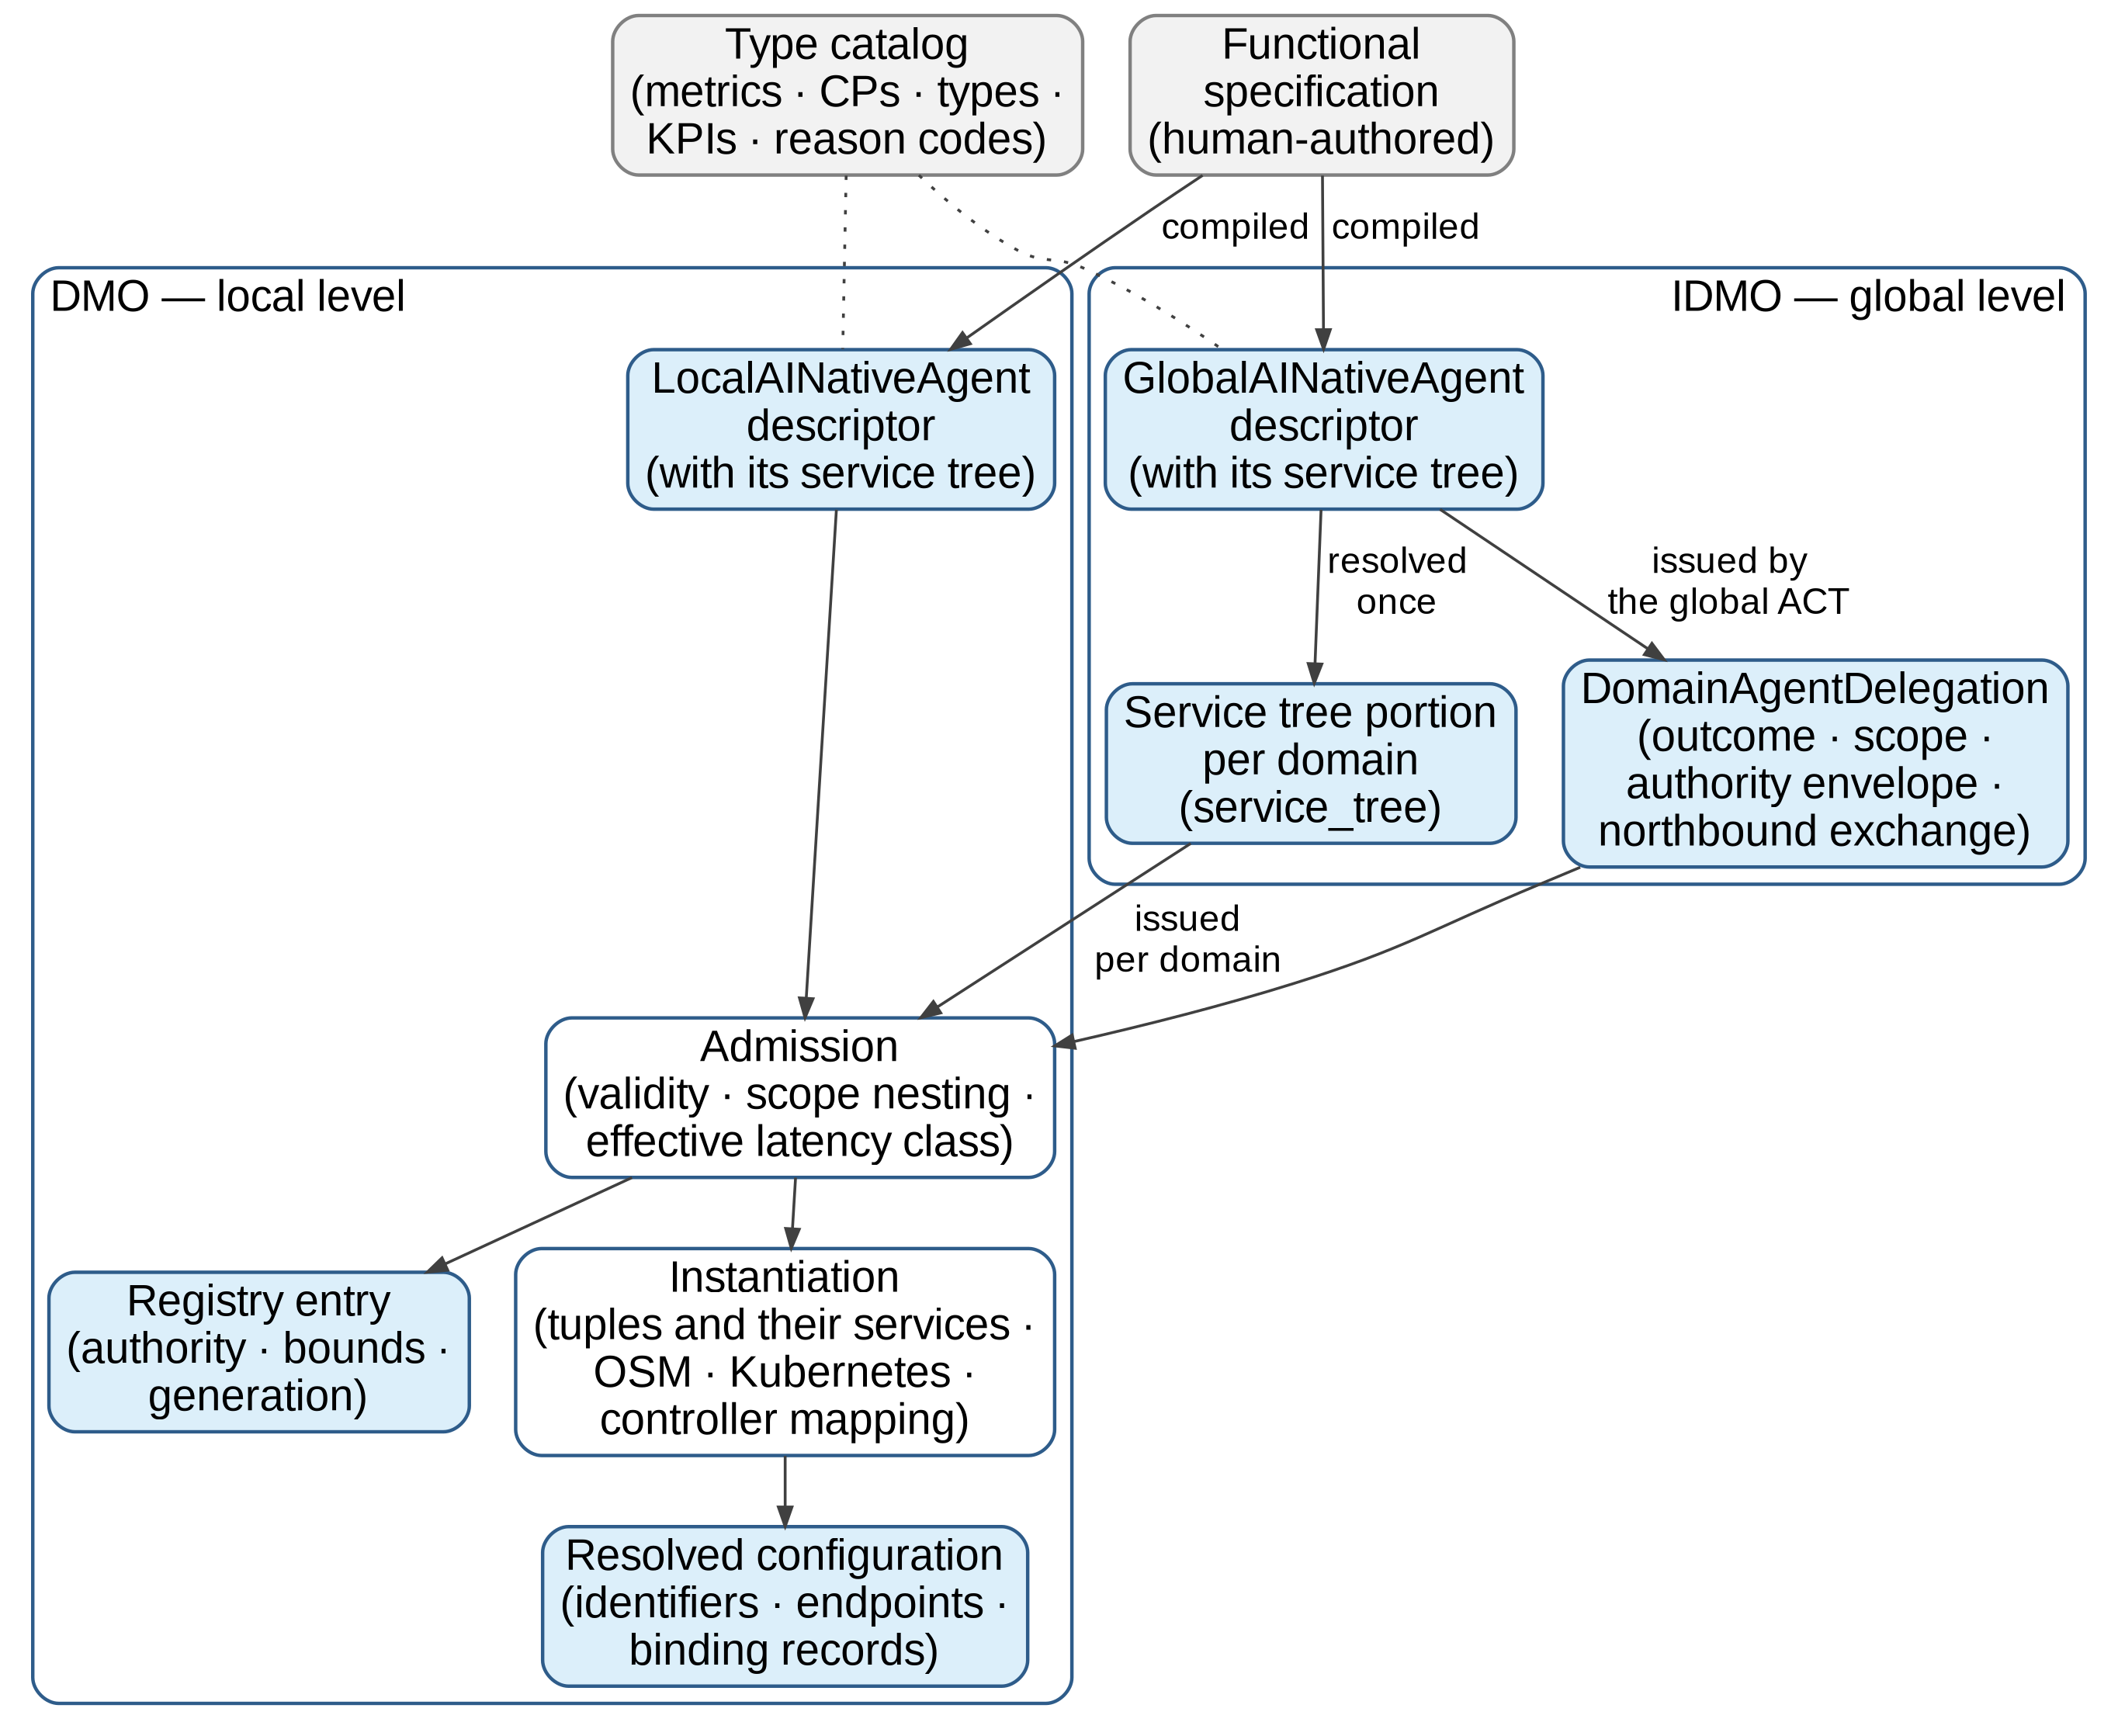
\includegraphics[width=\linewidth,height=0.45\textheight,keepaspectratio]{figures/image3.png}
\captionnum{3-3}
\caption{The descriptor chain at the global and local levels}
\label{fig:3-3}
\end{figure}

\hypertarget{descriptor-levels}{%
\subsubsection{Descriptor levels}\label{descriptor-levels}}

Agents are described at two levels. A LocalAINativeAgent descriptor,
owned by a DMO, describes a local agent and is specified field by field
in Sections 3.5.3 to 3.5.20. A GlobalAINativeAgent descriptor, owned by
the IDMO, describes a global agent and follows the same structure, with
four differences: its only domain is the IDMO; the controller binding of
its ACT is the IDMO's delegation interface towards the DMOs; its action
space consists of delegation operations --- create, update, approve,
suspend and terminate a delegation, and issue an intent to a DMO; and
its physical deployment addresses hosting at the IDMO only. A global
descriptor contains no domain-internal placement, network service
descriptor or controller mapping.

A third document, the DomainAgentDelegation, is not an agent descriptor.
It is the document by which the ACT of a global agent assigns an
outcome-oriented responsibility to one domain (Section 3.5.21).
Deployment translation --- to OSM, Kubernetes, Helm or controller
mappings --- belongs to the DMO and never appears in a global descriptor
or in a delegation.

\hypertarget{document-structure}{%
\subsubsection{Document structure}\label{document-structure}}

An agent descriptor consists of the sections of Table 3-13. The
applicability of each section depends on the composition class that the
platform derives from the tuple section. In the table, CL, OL, AN, OB
and AS denote the composition classes closed\_\allowbreak{}loop,
open\_\allowbreak{}loop, analytics, observation and
actuation\_\allowbreak{}service; M marks a mandatory section, C a
section required under the condition stated in its own table, O an
optional section, and a dash a section that shall be absent.

\begin{wptable}{3-13}\footnotesize

\begin{longtable}[]{@{}
  >{\raggedright\arraybackslash}p{(\columnwidth - 12\tabcolsep) * \real{0.2875}}
  >{\raggedright\arraybackslash}p{(\columnwidth - 12\tabcolsep) * \real{0.3375}}
  >{\raggedright\arraybackslash}p{(\columnwidth - 12\tabcolsep) * \real{0.0750}}
  >{\raggedright\arraybackslash}p{(\columnwidth - 12\tabcolsep) * \real{0.0750}}
  >{\raggedright\arraybackslash}p{(\columnwidth - 12\tabcolsep) * \real{0.0750}}
  >{\raggedright\arraybackslash}p{(\columnwidth - 12\tabcolsep) * \real{0.0750}}
  >{\raggedright\arraybackslash}p{(\columnwidth - 12\tabcolsep) * \real{0.0751}}@{}}
\caption{Sections of the agent descriptor}\tabularnewline
\toprule\noalign{}
\begin{minipage}[b]{\linewidth}\raggedright
\textbf{Section}
\end{minipage} & \begin{minipage}[b]{\linewidth}\raggedright
\textbf{Content}
\end{minipage} & \begin{minipage}[b]{\linewidth}\raggedright
\textbf{CL}
\end{minipage} & \begin{minipage}[b]{\linewidth}\raggedright
\textbf{OL}
\end{minipage} & \begin{minipage}[b]{\linewidth}\raggedright
\textbf{AN}
\end{minipage} & \begin{minipage}[b]{\linewidth}\raggedright
\textbf{OB}
\end{minipage} & \begin{minipage}[b]{\linewidth}\raggedright
\textbf{AS}
\end{minipage} \\
\midrule\noalign{}
\endfirsthead
\toprule\noalign{}
\begin{minipage}[b]{\linewidth}\raggedright
\textbf{Section}
\end{minipage} & \begin{minipage}[b]{\linewidth}\raggedright
\textbf{Content}
\end{minipage} & \begin{minipage}[b]{\linewidth}\raggedright
\textbf{CL}
\end{minipage} & \begin{minipage}[b]{\linewidth}\raggedright
\textbf{OL}
\end{minipage} & \begin{minipage}[b]{\linewidth}\raggedright
\textbf{AN}
\end{minipage} & \begin{minipage}[b]{\linewidth}\raggedright
\textbf{OB}
\end{minipage} & \begin{minipage}[b]{\linewidth}\raggedright
\textbf{AS}
\end{minipage} \\
\midrule\noalign{}
\endhead
\bottomrule\noalign{}
\endlastfoot
\textbf{schema\_\allowbreak{}version, kind} & Schema version;
LocalAINativeAgent or GlobalAINativeAgent & M & M & M & M & M \\
\textbf{identity} & Identity and publisher (Table 3-14) & M & M & M & M
& M \\
\textbf{tuple\_\allowbreak{}capabilities,
capability\_\allowbreak{}subsets, capability\_\allowbreak{}delegations}
& Capability modes, subsets and delegations (Table 3-15) & M & M & M & M
& M \\
\textbf{objectives} & Objective templates (Table 3-16) & M & M & --- &
--- & --- \\
\textbf{scope} & Primary and secondary domains, scope selectors,
observation and control scope (Table 3-17) & M & M & M & M & M \\
\textbf{action\_\allowbreak{}space} & Action types and their bounds
(Table 3-18) & M & M & --- & --- & M \\
\textbf{functions} & Per-capability function declarations (Tables 3-19
to 3-22) & M & M & M & M & M \\
\textbf{interfaces} & Flows, schemas, permitted bindings, exposed
contracts (Table 3-23) & M & M & M & M & M \\
\textbf{operations} & Operating mode, latency class, loop budget,
declared latencies (Table 3-24) & M & M & M & M & M \\
\textbf{physical\_\allowbreak{}deployment} & Allowed tiers, locations,
affinity, resources, state, artifacts, split deployment, migration
(Table 3-25) & M & M & M & M & M \\
\textbf{policies} & Authority mode, conflict resolution, priority,
mediation requests (Table 3-26) & M & --- & --- & --- & --- \\
\textbf{failure\_\allowbreak{}policy} & Per-capability failure behavior
(Table 3-27) & M & M & M & M & M \\
\textbf{model\_\allowbreak{}hooks} & Model artifacts, update policy,
drift signals, fallback (Table 3-28) & C & C & C & C & --- \\
\textbf{ownership, integrity} & Owner, stakeholder role, trust domain,
hash, signature, SBOM, platform dependencies (Table 3-29) & M & M & M &
M & M \\
\textbf{service\_\allowbreak{}tree} & Services required per tuple, tuple
bindings, domains of a global agent, operational timeout (Table 3-31) &
M & M & M & M & M \\
\textbf{x-*} & Extension fields (Section 3.5.17) & O & O & O & O & O \\
\end{longtable}

\end{wptable}

\hypertarget{identity}{%
\subsubsection{Identity}\label{identity}}

\begin{wptable}{3-14}

\begin{longtable}[]{@{}
  >{\raggedright\arraybackslash}p{(\columnwidth - 6\tabcolsep) * \real{0.2875}}
  >{\raggedright\arraybackslash}p{(\columnwidth - 6\tabcolsep) * \real{0.1438}}
  >{\raggedright\arraybackslash}p{(\columnwidth - 6\tabcolsep) * \real{0.0750}}
  >{\raggedright\arraybackslash}p{(\columnwidth - 6\tabcolsep) * \real{0.4937}}@{}}
\caption{Identity fields}\tabularnewline
\toprule\noalign{}
\begin{minipage}[b]{\linewidth}\raggedright
\textbf{Field}
\end{minipage} & \begin{minipage}[b]{\linewidth}\raggedright
\textbf{Type}
\end{minipage} & \begin{minipage}[b]{\linewidth}\raggedright
\textbf{Req.}
\end{minipage} & \begin{minipage}[b]{\linewidth}\raggedright
\textbf{Semantics and constraints}
\end{minipage} \\
\midrule\noalign{}
\endfirsthead
\toprule\noalign{}
\begin{minipage}[b]{\linewidth}\raggedright
\textbf{Field}
\end{minipage} & \begin{minipage}[b]{\linewidth}\raggedright
\textbf{Type}
\end{minipage} & \begin{minipage}[b]{\linewidth}\raggedright
\textbf{Req.}
\end{minipage} & \begin{minipage}[b]{\linewidth}\raggedright
\textbf{Semantics and constraints}
\end{minipage} \\
\midrule\noalign{}
\endhead
\bottomrule\noalign{}
\endlastfoot
\textbf{schema\_\allowbreak{}version} & semver & M & Version of the
descriptor schema; one of the versions the registry lists as
supported. \\
\textbf{kind} & enum & M & LocalAINativeAgent or GlobalAINativeAgent. \\
\textbf{identity.\allowbreak{}descriptor\_\allowbreak{}id} & id & M &
Stable URN of the agent type (Table 3-2). \\
\textbf{identity.\allowbreak{}version} & semver & M & Version of this
descriptor (Section 3.5.19). \\
\textbf{identity.\allowbreak{}agent\_\allowbreak{}version} & string & O
& Release identifier of the contributed logic, with build metadata;
informative, the artifact digests being authoritative. \\
\textbf{identity.name} & string & M & Human-readable name of at most 64
characters. \\
\textbf{identity.\allowbreak{}publisher\_\allowbreak{}identity} & string
& M & Organization contributing the agent, with its support channel;
resolves to a signing key in the agent\textquotesingle s trust
domain. \\
\textbf{identity.\allowbreak{}functional\_\allowbreak{}specification\_\allowbreak{}ref}
& string & O & Reference to the functional specification from which the
descriptor was compiled. \\
\textbf{identity.\allowbreak{}description} & string & O & Informative
text; not interpreted by the platform. \\
\textbf{identity.\allowbreak{}labels} & map & O & Discovery labels; not
interpreted by the platform. \\
\textbf{identity.\allowbreak{}license\_\allowbreak{}and\_\allowbreak{}ip}
& object & O & Licensing declaration: an SPDX license expression or
proprietary, and whether the artifacts are subject to export control;
not interpreted by admission. \\
\end{longtable}

\end{wptable}

\hypertarget{tuple-declaration-and-delegations}{%
\subsubsection{Tuple declaration and delegations}\label{tuple-declaration-and-delegations}}

The tuple sections declare the mode of each capability, the enumerated
subset of each partial capability and the provider of each delegated
capability (Table 3-15). The capability keys are MS, AE, DE and ACT.

\begin{wptable}{3-15}

\begin{longtable}[]{@{}
  >{\raggedright\arraybackslash}p{(\columnwidth - 6\tabcolsep) * \real{0.2875}}
  >{\raggedright\arraybackslash}p{(\columnwidth - 6\tabcolsep) * \real{0.1438}}
  >{\raggedright\arraybackslash}p{(\columnwidth - 6\tabcolsep) * \real{0.0750}}
  >{\raggedright\arraybackslash}p{(\columnwidth - 6\tabcolsep) * \real{0.4937}}@{}}
\caption{Tuple fields}\tabularnewline
\toprule\noalign{}
\begin{minipage}[b]{\linewidth}\raggedright
\textbf{Field}
\end{minipage} & \begin{minipage}[b]{\linewidth}\raggedright
\textbf{Type}
\end{minipage} & \begin{minipage}[b]{\linewidth}\raggedright
\textbf{Req.}
\end{minipage} & \begin{minipage}[b]{\linewidth}\raggedright
\textbf{Semantics and constraints}
\end{minipage} \\
\midrule\noalign{}
\endfirsthead
\toprule\noalign{}
\begin{minipage}[b]{\linewidth}\raggedright
\textbf{Field}
\end{minipage} & \begin{minipage}[b]{\linewidth}\raggedright
\textbf{Type}
\end{minipage} & \begin{minipage}[b]{\linewidth}\raggedright
\textbf{Req.}
\end{minipage} & \begin{minipage}[b]{\linewidth}\raggedright
\textbf{Semantics and constraints}
\end{minipage} \\
\midrule\noalign{}
\endhead
\bottomrule\noalign{}
\endlastfoot
\textbf{tuple\_\allowbreak{}capabilities.\allowbreak{}\textless cap\textgreater{}}
& enum & M & full, partial, delegated or none, for each of MS, AE, DE
and ACT. \\
\textbf{capability\_\allowbreak{}subsets.\allowbreak{}\textless cap\textgreater{}}
& list of type-ref & C & Required where the mode is partial. MS: metrics
or managed-object classes of the observation scope. AE: insight types.
DE: action types forming the decision space. ACT: action types
executed. \\
\textbf{capability\_\allowbreak{}delegations.\allowbreak{}\textless cap\textgreater.\allowbreak{}provider}
& id & C & Required where the mode is delegated, or the complement of a
partial subset is delegated. descriptor\_\allowbreak{}id of a provider
agent, or catalog identifier of a platform service or reused
capability. \\
\textbf{capability\_\allowbreak{}delegations.\allowbreak{}\textless cap\textgreater.\allowbreak{}covers}
& enum & C & Required where a provider is declared. all, where the
capability is delegated; complement, where the delegation covers the
complement of a partial subset. \\
\textbf{capability\_\allowbreak{}delegations.\allowbreak{}\textless cap\textgreater.\allowbreak{}interface}
& type-ref & C & Required where a provider is declared. Service contract
exposed by the provider. \\
\textbf{capability\_\allowbreak{}delegations.\allowbreak{}\textless cap\textgreater.\allowbreak{}interface\_\allowbreak{}profile}
& type-ref & C & Required where a provider is declared. Pinned interface
profile of the provider. \\
\textbf{capability\_\allowbreak{}delegations.\allowbreak{}\textless cap\textgreater.\allowbreak{}compatibility}
& semver-range & C & Required where a provider is declared. Accepted
provider versions; for a delegated AE, also the accepted model
versions. \\
\textbf{capability\_\allowbreak{}delegations.\allowbreak{}\textless cap\textgreater.\allowbreak{}sla\_\allowbreak{}assumptions}
& object & C & Required where a provider is declared. Maximum
99th-percentile latency and maximum age at delivery that the consumer
assumes of the provider; admission rejects a provider whose declared
figures exceed them. \\
\end{longtable}

\end{wptable}

A delegation pins the provider's interface profile and a range of
accepted provider versions. At admission the provider's declared scope
shall cover the consumer's, and the provider's declared latency and
freshness shall be within the consumer's SLA assumptions. At runtime the
provider's health and coverage are forwarded to the consumer as part of
the binding, and a provider whose published interface profile or version
leaves the pinned range raises a binding fault at the consumer, which
suspends the affected capability. A delegated ACT provider shall itself
satisfy every requirement on the ACT (Chapter 7).

\hypertarget{objectives}{%
\subsubsection{Objectives}\label{objectives}}

Objectives are declared as templates over KPIs of the catalog (Table
3-16). The target values of templates marked as bound by the request are
supplied when the descriptor is issued for instantiation, once, and are
fixed for the life of the instance; a change of target values is a new
agent (Section 3.5.20). At admission the platform registers the KPIs of
an agent's objectives with the conflict fabric as the KPI side of the
agent's registration (Chapter 10).

\begin{wptable}{3-16}

\begin{longtable}[]{@{}
  >{\raggedright\arraybackslash}p{(\columnwidth - 6\tabcolsep) * \real{0.2875}}
  >{\raggedright\arraybackslash}p{(\columnwidth - 6\tabcolsep) * \real{0.1438}}
  >{\raggedright\arraybackslash}p{(\columnwidth - 6\tabcolsep) * \real{0.0750}}
  >{\raggedright\arraybackslash}p{(\columnwidth - 6\tabcolsep) * \real{0.4937}}@{}}
\caption{Objective fields}\tabularnewline
\toprule\noalign{}
\begin{minipage}[b]{\linewidth}\raggedright
\textbf{Field in objectives{[}{]}}
\end{minipage} & \begin{minipage}[b]{\linewidth}\raggedright
\textbf{Type}
\end{minipage} & \begin{minipage}[b]{\linewidth}\raggedright
\textbf{Req.}
\end{minipage} & \begin{minipage}[b]{\linewidth}\raggedright
\textbf{Semantics and constraints}
\end{minipage} \\
\midrule\noalign{}
\endfirsthead
\toprule\noalign{}
\begin{minipage}[b]{\linewidth}\raggedright
\textbf{Field in objectives{[}{]}}
\end{minipage} & \begin{minipage}[b]{\linewidth}\raggedright
\textbf{Type}
\end{minipage} & \begin{minipage}[b]{\linewidth}\raggedright
\textbf{Req.}
\end{minipage} & \begin{minipage}[b]{\linewidth}\raggedright
\textbf{Semantics and constraints}
\end{minipage} \\
\midrule\noalign{}
\endhead
\bottomrule\noalign{}
\endlastfoot
\textbf{objective\_\allowbreak{}id} & string & M & Unique within the
descriptor. \\
\textbf{kpi} & type-ref & M & Objective KPI of the catalog, with its
unit and measurement methodology. \\
\textbf{direction} & enum & M & minimize, maximize,
hold\_\allowbreak{}below, hold\_\allowbreak{}above or
hold\_\allowbreak{}within.\allowbreak{} \\
\textbf{target} & object & M & from\_\allowbreak{}request, bound when
the descriptor is issued for instantiation; or a fixed value in the
KPI\textquotesingle s unit --- a pair of values for
hold\_\allowbreak{}within.\allowbreak{} \\
\textbf{evaluation\_\allowbreak{}window} & duration & M & Window over
which objective status is evaluated for assurance. \\
\textbf{at\_\allowbreak{}risk\_\allowbreak{}margin} & ratio & M &
Fraction of the target within which the status is at-risk rather than
met. \\
\textbf{rank} & integer & O & Order among the agent\textquotesingle s
own objectives, 1 highest; used by its DE only, with no effect on
arbitration priority. \\
\end{longtable}

\end{wptable}

Objective status is evaluated over the evaluation window. For a
hold\_\allowbreak{}below objective with target T and at-risk margin m,
the status is \emph{met} while the KPI does not exceed T(1 − m),
\emph{at-risk} while it lies above T(1 − m) and at most T, and
\emph{not-met} above T. A hold\_\allowbreak{}above objective is
evaluated symmetrically, and a hold\_\allowbreak{}within objective
applies both conditions to its two targets. A minimize or maximize
objective with a target is evaluated as hold\_\allowbreak{}below or
hold\_\allowbreak{}above respectively; without a target it has no status
and serves only the agent's own DE.

\hypertarget{scope}{%
\subsubsection{Scope}\label{scope}}

\begin{wptable}{3-17}

\begin{longtable}[]{@{}
  >{\raggedright\arraybackslash}p{(\columnwidth - 6\tabcolsep) * \real{0.2875}}
  >{\raggedright\arraybackslash}p{(\columnwidth - 6\tabcolsep) * \real{0.1438}}
  >{\raggedright\arraybackslash}p{(\columnwidth - 6\tabcolsep) * \real{0.0750}}
  >{\raggedright\arraybackslash}p{(\columnwidth - 6\tabcolsep) * \real{0.4937}}@{}}
\caption{Scope fields}\tabularnewline
\toprule\noalign{}
\begin{minipage}[b]{\linewidth}\raggedright
\textbf{Field in scope}
\end{minipage} & \begin{minipage}[b]{\linewidth}\raggedright
\textbf{Type}
\end{minipage} & \begin{minipage}[b]{\linewidth}\raggedright
\textbf{Req.}
\end{minipage} & \begin{minipage}[b]{\linewidth}\raggedright
\textbf{Semantics and constraints}
\end{minipage} \\
\midrule\noalign{}
\endfirsthead
\toprule\noalign{}
\begin{minipage}[b]{\linewidth}\raggedright
\textbf{Field in scope}
\end{minipage} & \begin{minipage}[b]{\linewidth}\raggedright
\textbf{Type}
\end{minipage} & \begin{minipage}[b]{\linewidth}\raggedright
\textbf{Req.}
\end{minipage} & \begin{minipage}[b]{\linewidth}\raggedright
\textbf{Semantics and constraints}
\end{minipage} \\
\midrule\noalign{}
\endhead
\bottomrule\noalign{}
\endlastfoot
\textbf{primary\_\allowbreak{}domain} & enum & M & Domain of Table 3-10
in which the agent observes and acts; idmo for a global agent. \\
\textbf{secondary\_\allowbreak{}domains} & list of enum & C & Required
where a delegation crosses a domain boundary. Domains of the providers
of the agent\textquotesingle s cross-domain delegations (Section 3.3.5),
listed exactly: the domains of AE providers, and idmo where the DE is
delegated to the agent\textquotesingle s global agent. They are never
part of the control scope. \\
\textbf{scope\_\allowbreak{}selectors} & list of enum & M & Selector
dimensions in which the concrete scope of an instance is expressed and
which every message carries as scope tags: any of region, site, slice,
tenant and technology. \\
\textbf{observation\_\allowbreak{}scope.\allowbreak{}object\_\allowbreak{}classes}
& list of enum & C & Required where the MS or the AE is not none.
Managed-object classes observed: node, link, path, slice, flow, service,
ue, device; delegation for a global agent. \\
\textbf{observation\_\allowbreak{}scope.\allowbreak{}metrics} & list of
type-ref & C & Required where the MS is not none. Catalog metrics
observed. \\
\textbf{control\_\allowbreak{}scope.\allowbreak{}object\_\allowbreak{}classes}
& list of enum & C & Required where the DE or the ACT is not none.
Managed-object classes whose parameters may change. \\
\textbf{control\_\allowbreak{}scope.\allowbreak{}control\_\allowbreak{}parameters}
& list of type-ref & C & Required where the DE or the ACT is not none.
Catalog control parameters that may change. \\
\textbf{max\_\allowbreak{}objects} & integer & O & Upper bound on the
number of managed objects an instance may be granted; admission rejects
an instantiation that exceeds it. \\
\end{longtable}

\end{wptable}

Scopes nest. For every agent the control scope shall be contained in the
observation-justified scope, which shall be contained in the declared
domain scope, which shall be contained in the agent's trust domain. The
observation-justified scope comprises the managed-object classes for
which the agent's evidence --- its own MS, or a delegated MS or AE ---
includes at least one metric: an agent shall not change what it cannot
observe. At instantiation the declared scopes are bound to concrete
identifiers, once, and the same nesting shall hold for those
identifiers.

\hypertarget{action-space}{%
\subsubsection{Action space}\label{action-space}}

The action space is the set of actions the agent may request. It is the
object on which most of the framework's bounds act: the egress gate of
the DE, the registration with the conflict fabric, the last-mile check
of the ACT and the platform's stability enforcement all apply to it.
Each action type of the catalog that the agent may request appears once
in the action space, with the attributes of Table 3-18.

\begin{wptable}{3-18}

\begin{longtable}[]{@{}
  >{\raggedright\arraybackslash}p{(\columnwidth - 6\tabcolsep) * \real{0.2875}}
  >{\raggedright\arraybackslash}p{(\columnwidth - 6\tabcolsep) * \real{0.1438}}
  >{\raggedright\arraybackslash}p{(\columnwidth - 6\tabcolsep) * \real{0.0750}}
  >{\raggedright\arraybackslash}p{(\columnwidth - 6\tabcolsep) * \real{0.4937}}@{}}
\caption{Action space fields, per action type}\tabularnewline
\toprule\noalign{}
\begin{minipage}[b]{\linewidth}\raggedright
\textbf{Field}
\end{minipage} & \begin{minipage}[b]{\linewidth}\raggedright
\textbf{Type}
\end{minipage} & \begin{minipage}[b]{\linewidth}\raggedright
\textbf{Req.}
\end{minipage} & \begin{minipage}[b]{\linewidth}\raggedright
\textbf{Semantics and constraints}
\end{minipage} \\
\midrule\noalign{}
\endfirsthead
\toprule\noalign{}
\begin{minipage}[b]{\linewidth}\raggedright
\textbf{Field}
\end{minipage} & \begin{minipage}[b]{\linewidth}\raggedright
\textbf{Type}
\end{minipage} & \begin{minipage}[b]{\linewidth}\raggedright
\textbf{Req.}
\end{minipage} & \begin{minipage}[b]{\linewidth}\raggedright
\textbf{Semantics and constraints}
\end{minipage} \\
\midrule\noalign{}
\endhead
\bottomrule\noalign{}
\endlastfoot
\textbf{action\_\allowbreak{}type} & type-ref & M & Catalog action
type. \\
\textbf{targets} & object & M & Managed-object class and control
parameters changed; contained in the control scope. \\
\textbf{parameter\_\allowbreak{}bounds} & map & M & For each parameter:
minimum, maximum and step, or an enumeration of permitted values. \\
\textbf{rate\_\allowbreak{}limit} & rate & M & Maximum number of
executions per target. \\
\textbf{stability.\allowbreak{}cooldown} & duration & M & Minimum
interval between two executions on the same target. \\
\textbf{stability.\allowbreak{}minimum\_\allowbreak{}hold\_\allowbreak{}time}
& duration & M & Minimum time a change remains in effect on a target
before an execution that reverses it. \\
\textbf{stability.\allowbreak{}max\_\allowbreak{}step} & map & O &
Maximum change of each parameter in one execution. \\
\textbf{stability.\allowbreak{}staging} & list & O & Ordered stages,
each with a fraction of the targets and a dwell time, for changes
applied progressively. \\
\textbf{preconditions} & list of predicate & O & Conditions on the state
of the target, evaluated by the ACT runtime before submission. \\
\textbf{verification.\allowbreak{}method} & enum & M &
ms\_\allowbreak{}observation,
controller\_\allowbreak{}state\_\allowbreak{}query or unverifiable. \\
\textbf{verification.\allowbreak{}timing} & enum & C & Required where
the method is not unverifiable. in\_\allowbreak{}band or deferred. \\
\textbf{verification.\allowbreak{}deadline} & duration & C & Required
where the timing is deferred. Deadline within which deferred
verification completes. \\
\textbf{idempotency} & enum & M & idempotent or
non\_\allowbreak{}idempotent.\allowbreak{} \\
\textbf{rollback} & enum & M & supported, using the rollback method of
the catalog entry; or not\_\allowbreak{}supported.\allowbreak{} \\
\textbf{mediation\_\allowbreak{}path} & enum & M & envelope, policy or
mediated: the path by which the action is expected to be authorized
(Section 3.9.2). \\
\end{longtable}

\end{wptable}

An action type whose effect cannot be verified through a path
independent of the controller's acknowledgement is declared with the
verification method unverifiable. Such an action type is admitted only
with targets enumerated individually at instantiation rather than by
class, with a rate limit no higher than the ceiling for unverifiable
execution that its catalog entry sets, with every execution reported to
the DMO as it occurs, and under elevated evaluation scrutiny. These
restrictions bound where and how often such an action is taken; they do
not lower the authority of the agent that takes it, and an agent at
closed\_\allowbreak{}loop\_\allowbreak{}full executes an unverifiable
action type within them without approval. Its outcome is never
ACKNOWLEDGED\_\allowbreak{}VERIFIED.\allowbreak{}

\hypertarget{capability-functions}{%
\subsubsection{Capability functions}\label{capability-functions}}

The functions section declares, for each capability whose mode is full
or partial, how its contributed logic is invoked and what it consumes
and produces. Every capability section contains a technique class, a
trigger, a maximum concurrency where applicable and an opaque parameters
block. The parameters block configures the contributed logic, is not
interpreted by the platform and does not make the descriptor an
extension. The capability-specific fields are listed in Tables 3-19 to
3-22 and their behavior is specified in the capability chapters.

\begin{wptable}{3-19}

\begin{longtable}[]{@{}
  >{\raggedright\arraybackslash}p{(\columnwidth - 6\tabcolsep) * \real{0.2875}}
  >{\raggedright\arraybackslash}p{(\columnwidth - 6\tabcolsep) * \real{0.1438}}
  >{\raggedright\arraybackslash}p{(\columnwidth - 6\tabcolsep) * \real{0.0750}}
  >{\raggedright\arraybackslash}p{(\columnwidth - 6\tabcolsep) * \real{0.4937}}@{}}
\caption{Monitoring System function fields}\tabularnewline
\toprule\noalign{}
\begin{minipage}[b]{\linewidth}\raggedright
\textbf{Field in functions.MS}
\end{minipage} & \begin{minipage}[b]{\linewidth}\raggedright
\textbf{Type}
\end{minipage} & \begin{minipage}[b]{\linewidth}\raggedright
\textbf{Req.}
\end{minipage} & \begin{minipage}[b]{\linewidth}\raggedright
\textbf{Semantics and constraints}
\end{minipage} \\
\midrule\noalign{}
\endfirsthead
\toprule\noalign{}
\begin{minipage}[b]{\linewidth}\raggedright
\textbf{Field in functions.MS}
\end{minipage} & \begin{minipage}[b]{\linewidth}\raggedright
\textbf{Type}
\end{minipage} & \begin{minipage}[b]{\linewidth}\raggedright
\textbf{Req.}
\end{minipage} & \begin{minipage}[b]{\linewidth}\raggedright
\textbf{Semantics and constraints}
\end{minipage} \\
\midrule\noalign{}
\endhead
\bottomrule\noalign{}
\endlastfoot
\textbf{technique} & enum & M & Technique class (Table 3-11). \\
\textbf{observation\_\allowbreak{}contract} & schema-ref & M & Schema of
the observation records; contains no model outputs, scores or confidence
fields. \\
\textbf{metrics{[}{]}} & list & M & For each metric: the catalog entry;
its measurement kind, matching the entry (Table 4-1); unit; sampling
(period, on\_\allowbreak{}change or event); aggregation over the window
(none, sum, count, duration, min, max, mean, p50, p95 or p99), permitted
for the kind (Annex B); the window, where the aggregation is not none;
and, for a computed metric not defined by its catalog entry, the
structured derivation of Section 4.4. \\
\textbf{sources{[}{]}} & list & M & Sources read, in precedence order,
each with its catalog source kind, such as E2 KPM, controller telemetry,
gNMI, SNMP, Prometheus or NGSI-LD context brokers, and its acquisition
pattern (Table 4-2); access is read-only. \\
\textbf{trigger} & object & M & periodic, with a period; event, with the
triggering source; schedule, with a cron expression in UTC; or request,
received through an exposed contract. \\
\textbf{data\_\allowbreak{}quality\_\allowbreak{}signals} & list of enum
& M & Quality signals produced: loss and delivery\_\allowbreak{}latency
at least; sampling\_\allowbreak{}policy,
aggregation\_\allowbreak{}policy and jitter as applicable. \\
\textbf{max\_\allowbreak{}concurrency} & integer & O & Concurrent
invocations; default 1. \\
\textbf{parameters} & object & O & Opaque configuration of the
contributed logic. \\
\end{longtable}

\end{wptable}

\begin{wptable}{3-20}

\begin{longtable}[]{@{}
  >{\raggedright\arraybackslash}p{(\columnwidth - 6\tabcolsep) * \real{0.2875}}
  >{\raggedright\arraybackslash}p{(\columnwidth - 6\tabcolsep) * \real{0.1438}}
  >{\raggedright\arraybackslash}p{(\columnwidth - 6\tabcolsep) * \real{0.0750}}
  >{\raggedright\arraybackslash}p{(\columnwidth - 6\tabcolsep) * \real{0.4937}}@{}}
\caption{Analytics Engine function fields}\tabularnewline
\toprule\noalign{}
\begin{minipage}[b]{\linewidth}\raggedright
\textbf{Field in functions.AE}
\end{minipage} & \begin{minipage}[b]{\linewidth}\raggedright
\textbf{Type}
\end{minipage} & \begin{minipage}[b]{\linewidth}\raggedright
\textbf{Req.}
\end{minipage} & \begin{minipage}[b]{\linewidth}\raggedright
\textbf{Semantics and constraints}
\end{minipage} \\
\midrule\noalign{}
\endfirsthead
\toprule\noalign{}
\begin{minipage}[b]{\linewidth}\raggedright
\textbf{Field in functions.AE}
\end{minipage} & \begin{minipage}[b]{\linewidth}\raggedright
\textbf{Type}
\end{minipage} & \begin{minipage}[b]{\linewidth}\raggedright
\textbf{Req.}
\end{minipage} & \begin{minipage}[b]{\linewidth}\raggedright
\textbf{Semantics and constraints}
\end{minipage} \\
\midrule\noalign{}
\endhead
\bottomrule\noalign{}
\endlastfoot
\textbf{technique} & enum & M & Technique class (Table 3-11). \\
\textbf{insight\_\allowbreak{}types} & list of type-ref & M & Insight
types produced, each with its schema. \\
\textbf{inputs} & object & M & Observations or data products consumed,
and the feature set with its version. \\
\textbf{serving\_\allowbreak{}mode} & enum & M & streaming, through a
serving endpoint; or batch, as a job. \\
\textbf{validity\_\allowbreak{}conditions} & list of predicate & C &
Required where a model is used. Conditions over input features under
which the model\textquotesingle s output is valid. \\
\textbf{models} & list of string & C & Required where a model is used.
Model identifiers of entries of
model\_\allowbreak{}hooks.\allowbreak{}model\_\allowbreak{}artifacts.\allowbreak{} \\
\textbf{fallback} & object & O & Declared fallback heuristic, used only
where the failure policy selects
declared\_\allowbreak{}fallback.\allowbreak{} \\
\textbf{trigger} & object & M & Input arrival, with a batching window;
periodic; schedule; or request, received through an exposed contract. \\
\textbf{max\_\allowbreak{}concurrency, parameters} & integer, object & O
& As for the MS. \\
\end{longtable}

\end{wptable}

\begin{wptable}{3-21}

\begin{longtable}[]{@{}
  >{\raggedright\arraybackslash}p{(\columnwidth - 6\tabcolsep) * \real{0.2875}}
  >{\raggedright\arraybackslash}p{(\columnwidth - 6\tabcolsep) * \real{0.1438}}
  >{\raggedright\arraybackslash}p{(\columnwidth - 6\tabcolsep) * \real{0.0750}}
  >{\raggedright\arraybackslash}p{(\columnwidth - 6\tabcolsep) * \real{0.4937}}@{}}
\caption{Decision Engine function fields}\tabularnewline
\toprule\noalign{}
\begin{minipage}[b]{\linewidth}\raggedright
\textbf{Field in functions.DE}
\end{minipage} & \begin{minipage}[b]{\linewidth}\raggedright
\textbf{Type}
\end{minipage} & \begin{minipage}[b]{\linewidth}\raggedright
\textbf{Req.}
\end{minipage} & \begin{minipage}[b]{\linewidth}\raggedright
\textbf{Semantics and constraints}
\end{minipage} \\
\midrule\noalign{}
\endfirsthead
\toprule\noalign{}
\begin{minipage}[b]{\linewidth}\raggedright
\textbf{Field in functions.DE}
\end{minipage} & \begin{minipage}[b]{\linewidth}\raggedright
\textbf{Type}
\end{minipage} & \begin{minipage}[b]{\linewidth}\raggedright
\textbf{Req.}
\end{minipage} & \begin{minipage}[b]{\linewidth}\raggedright
\textbf{Semantics and constraints}
\end{minipage} \\
\midrule\noalign{}
\endhead
\bottomrule\noalign{}
\endlastfoot
\textbf{technique} & enum & M & Technique class (Table 3-11). \\
\textbf{inputs} & list of type-ref & M & Insight types consumed;
observation metrics where the AE is none. \\
\textbf{min\_\allowbreak{}input\_\allowbreak{}coverage} & ratio & M &
Input coverage below which the degraded-evidence behavior executes. \\
\textbf{confidence\_\allowbreak{}threshold} & ratio & M & Decision
confidence below which the low-confidence behavior executes. \\
\textbf{interpretable} & bool & M & Whether the decision logic can
produce, for an individual decision, an account of which inputs
determined the outcome and in what direction, supplied with the
rationale on request (Chapter 6). Where false, the authority ceiling is
closed\_\allowbreak{}loop\_\allowbreak{}reduced (V-30). \\
\textbf{reason\_\allowbreak{}codes} & list of type-ref & M & Catalog
reason codes the DE may place in a rationale. \\
\textbf{constraints} & list of predicate & M & Constraints the DE holds
itself to in forming intents; may be empty. \\
\textbf{intent\_\allowbreak{}validity} & duration & M & Longest validity
window an emitted intent may carry; the validity\_\allowbreak{}window of
every intent envelope lies within it. \\
\textbf{tools} & list of type-ref & C & Required where the technique is
generative. Read-only tools the contributed logic may call. \\
\textbf{models} & list of string & C & Required where a model is used.
As for the AE. \\
\textbf{trigger} & object & M & Insight arrival, periodic or schedule,
or a combination of them; outcomes, verdict expiries and notifications
from the conflict fabric also trigger a cycle. \\
\textbf{parameters} & object & O & Opaque configuration of the
contributed logic. \\
\end{longtable}

\end{wptable}

\begin{wptable}{3-22}

\begin{longtable}[]{@{}
  >{\raggedright\arraybackslash}p{(\columnwidth - 6\tabcolsep) * \real{0.2875}}
  >{\raggedright\arraybackslash}p{(\columnwidth - 6\tabcolsep) * \real{0.1438}}
  >{\raggedright\arraybackslash}p{(\columnwidth - 6\tabcolsep) * \real{0.0750}}
  >{\raggedright\arraybackslash}p{(\columnwidth - 6\tabcolsep) * \real{0.4937}}@{}}
\caption{Actuator function fields}\tabularnewline
\toprule\noalign{}
\begin{minipage}[b]{\linewidth}\raggedright
\textbf{Field in functions.ACT}
\end{minipage} & \begin{minipage}[b]{\linewidth}\raggedright
\textbf{Type}
\end{minipage} & \begin{minipage}[b]{\linewidth}\raggedright
\textbf{Req.}
\end{minipage} & \begin{minipage}[b]{\linewidth}\raggedright
\textbf{Semantics and constraints}
\end{minipage} \\
\midrule\noalign{}
\endfirsthead
\toprule\noalign{}
\begin{minipage}[b]{\linewidth}\raggedright
\textbf{Field in functions.ACT}
\end{minipage} & \begin{minipage}[b]{\linewidth}\raggedright
\textbf{Type}
\end{minipage} & \begin{minipage}[b]{\linewidth}\raggedright
\textbf{Req.}
\end{minipage} & \begin{minipage}[b]{\linewidth}\raggedright
\textbf{Semantics and constraints}
\end{minipage} \\
\midrule\noalign{}
\endhead
\bottomrule\noalign{}
\endlastfoot
\textbf{technique} & enum & M & deterministic, or optimization with
deterministic execution. \\
\textbf{controller\_\allowbreak{}binding} & type-ref & M & Catalog
controller binding: for example the TeraFlowSDN northbound interface,
E2SM-RC through the Near-RT RIC, O1, the OSM or DMO lifecycle interface,
or the IDMO delegation interface for a global agent. \\
\textbf{interface\_\allowbreak{}profile} & type-ref & M & Pinned version
of the controller interface. \\
\textbf{compatibility} & semver-range & M & Accepted controller
interface versions; a controller outside the range raises a binding
fault. \\
\textbf{executes} & list of type-ref & M & Action types executed;
contained in the action space. \\
\textbf{actuation\_\allowbreak{}timeout} & duration & M & Time after
submission beyond which a transaction is UNRESOLVED. \\
\textbf{max\_\allowbreak{}concurrency} & integer & O & Concurrent
transactions on distinct targets; default 1. \\
\textbf{parameters} & object & O & Opaque configuration of the
translation logic. \\
\end{longtable}

\end{wptable}

\hypertarget{interfaces}{%
\subsubsection{Interfaces}\label{interfaces}}

The interfaces section declares, for each logical flow of the agent, the
schema of its semantic object, the binding classes permitted for it and
the delivery guarantee it requires (Chapter 8), and, for an agent that
acts as a provider, the service contracts it exposes (Table 3-23). The
binding class of each edge is selected by the DMO at realization from
the classes the descriptor permits. The classes that may be permitted
for each flow are:

\begin{itemize}
\tightlist
\item
  OBSERVATION --- LOCAL\_\allowbreak{}RUNTIME, or
  DATA\_\allowbreak{}CONTINUUM as a governed stream; never SMB;
\item
  INSIGHT --- LOCAL\_\allowbreak{}RUNTIME; SMB for compact insight
  consumed across a runtime boundary; DATA\_\allowbreak{}CONTINUUM for
  derived artifacts such as features, embeddings and series;
\item
  INTENT --- LOCAL\_\allowbreak{}RUNTIME or SMB;
\item
  OUTCOME --- LOCAL\_\allowbreak{}RUNTIME or SMB, delivered to the DE
  and to the DMO;
\item
  the ACT's interaction with its controller --- SOUTHBOUND only, always
  request-response.
\end{itemize}

An SMB message carries control and coordination content only. It may
reference a data product but never carries one. A request to an exposed
contract with the request\_\allowbreak{}response pattern is a control
message on the SMB, and its result is returned on a binding permitted
for the flow of that contract.

\begin{wptable}{3-23}

\begin{longtable}[]{@{}
  >{\raggedright\arraybackslash}p{(\columnwidth - 6\tabcolsep) * \real{0.2875}}
  >{\raggedright\arraybackslash}p{(\columnwidth - 6\tabcolsep) * \real{0.1438}}
  >{\raggedright\arraybackslash}p{(\columnwidth - 6\tabcolsep) * \real{0.0750}}
  >{\raggedright\arraybackslash}p{(\columnwidth - 6\tabcolsep) * \real{0.4937}}@{}}
\caption{Interface fields}\tabularnewline
\toprule\noalign{}
\begin{minipage}[b]{\linewidth}\raggedright
\textbf{Field in interfaces}
\end{minipage} & \begin{minipage}[b]{\linewidth}\raggedright
\textbf{Type}
\end{minipage} & \begin{minipage}[b]{\linewidth}\raggedright
\textbf{Req.}
\end{minipage} & \begin{minipage}[b]{\linewidth}\raggedright
\textbf{Semantics and constraints}
\end{minipage} \\
\midrule\noalign{}
\endfirsthead
\toprule\noalign{}
\begin{minipage}[b]{\linewidth}\raggedright
\textbf{Field in interfaces}
\end{minipage} & \begin{minipage}[b]{\linewidth}\raggedright
\textbf{Type}
\end{minipage} & \begin{minipage}[b]{\linewidth}\raggedright
\textbf{Req.}
\end{minipage} & \begin{minipage}[b]{\linewidth}\raggedright
\textbf{Semantics and constraints}
\end{minipage} \\
\midrule\noalign{}
\endhead
\bottomrule\noalign{}
\endlastfoot
\textbf{flows{[}{]}.flow} & enum & M & OBSERVATION, INSIGHT, INTENT or
OUTCOME. \\
\textbf{flows{[}{]}.from, flows{[}{]}.to} & enum & M & Producing and
consuming capability, or a provider or consumer outside the agent. \\
\textbf{flows{[}{]}.schema} & schema-ref & M & Semantic schema of the
flow\textquotesingle s object. \\
\textbf{flows{[}{]}.\allowbreak{}binding\_\allowbreak{}classes} & list
of enum & M & Permitted binding classes, within those allowed for the
flow (Section 3.5.10). \\
\textbf{flows{[}{]}.\allowbreak{}max\_\allowbreak{}rate} & rate & M &
Maximum rate at which the producer emits. \\
\textbf{flows{[}{]}.freshness} & duration & M & Maximum age at delivery
for the consumer to accept the object. \\
\textbf{flows{[}{]}.\allowbreak{}delivery\_\allowbreak{}guarantee} &
enum & M & at\_\allowbreak{}most\_\allowbreak{}once,
at\_\allowbreak{}least\_\allowbreak{}once or exactly\_\allowbreak{}once
(Chapter 8). exactly\_\allowbreak{}once is not permitted for an
OBSERVATION flow, and an INTENT flow toward an action type declared
non\_\allowbreak{}idempotent is not
at\_\allowbreak{}least\_\allowbreak{}once.\allowbreak{} \\
\textbf{flows{[}{]}.\allowbreak{}latency\_\allowbreak{}bound} & object &
C & Required where the agent is of the real\_\allowbreak{}time class and
the flow permits a binding class other than
LOCAL\_\allowbreak{}RUNTIME.\allowbreak{} The 99th-percentile latency
the flow achieves, with a reference to its evidence: a measurement on
the proposed placement or a commitment of the transport that carries it
(Section 3.8.3). \\
\textbf{data\_\allowbreak{}products{[}{]}} & object & C & Required where
DATA\_\allowbreak{}CONTINUUM is permitted for a flow. Data product
identifier and the NGSI-LD entity type onto which the schema maps. \\
\textbf{exposed{[}{]}} & object & C & Required where the agent is a
provider. Exposed contract: identifier, flow, schema, interaction
pattern --- publish or request\_\allowbreak{}response --- interface
profile, and the trust domains permitted to consume it. \\
\end{longtable}

\end{wptable}

\hypertarget{operations}{%
\subsubsection{Operations}\label{operations}}

The operations section declares what starts the agent's cycles and the
timing the agent commits to (Table 3-24). The operating mode states what
starts a cycle: a continuous agent is driven by a periodic trigger, an
event-driven agent by events or by the arrival of its inputs, a
scheduled agent by a schedule, and an on-demand agent by requests
received through a contract it exposes with the
request\_\allowbreak{}response pattern (Section 3.5.10). The requester
is unconstrained by the framework and is not declared: a deliberate
operator-triggered intervention, another agent that needs this agent's
output, or an orchestration or service function that determines that the
agent is required. The operating mode governs what starts a cycle and
nothing else; an on-demand agent of any composition class is bound by
the same authority ceiling, the same mediation and the same action space
as any other agent once its cycle begins. The trigger of the agent's
entry capability --- the first of its MS, AE and DE whose mode is full
or partial --- agrees with the mode (Table 3-30). Between the runs of a
scheduled agent and between the requests to an on-demand agent, its
capabilities remain instantiated and keep their authority state.

\begin{wptable}{3-24}

\begin{longtable}[]{@{}
  >{\raggedright\arraybackslash}p{(\columnwidth - 6\tabcolsep) * \real{0.2875}}
  >{\raggedright\arraybackslash}p{(\columnwidth - 6\tabcolsep) * \real{0.1438}}
  >{\raggedright\arraybackslash}p{(\columnwidth - 6\tabcolsep) * \real{0.0750}}
  >{\raggedright\arraybackslash}p{(\columnwidth - 6\tabcolsep) * \real{0.4937}}@{}}
\caption{Operations fields}\tabularnewline
\toprule\noalign{}
\begin{minipage}[b]{\linewidth}\raggedright
\textbf{Field in operations}
\end{minipage} & \begin{minipage}[b]{\linewidth}\raggedright
\textbf{Type}
\end{minipage} & \begin{minipage}[b]{\linewidth}\raggedright
\textbf{Req.}
\end{minipage} & \begin{minipage}[b]{\linewidth}\raggedright
\textbf{Semantics and constraints}
\end{minipage} \\
\midrule\noalign{}
\endfirsthead
\toprule\noalign{}
\begin{minipage}[b]{\linewidth}\raggedright
\textbf{Field in operations}
\end{minipage} & \begin{minipage}[b]{\linewidth}\raggedright
\textbf{Type}
\end{minipage} & \begin{minipage}[b]{\linewidth}\raggedright
\textbf{Req.}
\end{minipage} & \begin{minipage}[b]{\linewidth}\raggedright
\textbf{Semantics and constraints}
\end{minipage} \\
\midrule\noalign{}
\endhead
\bottomrule\noalign{}
\endlastfoot
\textbf{mode} & enum & M & continuous, event\_\allowbreak{}driven,
scheduled or on\_\allowbreak{}demand: what starts the
agent\textquotesingle s cycles (Section 3.5.11). \\
\textbf{latency\_\allowbreak{}class} & enum & M &
real\_\allowbreak{}time, near\_\allowbreak{}real\_\allowbreak{}time,
non\_\allowbreak{}real\_\allowbreak{}time or offline. \\
\textbf{loop\_\allowbreak{}budget} & duration & C & Required where the
class is not offline. Within the range of the class (Table 3-37). \\
\textbf{class\_\allowbreak{}policy} & enum & M &
accept\_\allowbreak{}lower or
reject\_\allowbreak{}if\_\allowbreak{}unmet (Section 3.8.3). \\
\textbf{latency\_\allowbreak{}p99.\allowbreak{}\textless cap\textgreater{}}
& duration & M & Mandatory for every capability whose mode is not none.
Declared 99th-percentile latency. MS: from the close of the window to
publication. AE and DE: from invocation to return. ACT: from receipt of
the intent to the controller\textquotesingle s acknowledgement. \\
\end{longtable}

\end{wptable}

\hypertarget{physical-deployment}{%
\subsubsection{Physical deployment}\label{physical-deployment}}

\begin{wptable}{3-25}

\begin{longtable}[]{@{}
  >{\raggedright\arraybackslash}p{(\columnwidth - 6\tabcolsep) * \real{0.2875}}
  >{\raggedright\arraybackslash}p{(\columnwidth - 6\tabcolsep) * \real{0.1438}}
  >{\raggedright\arraybackslash}p{(\columnwidth - 6\tabcolsep) * \real{0.0750}}
  >{\raggedright\arraybackslash}p{(\columnwidth - 6\tabcolsep) * \real{0.4937}}@{}}
\caption{Physical deployment fields}\tabularnewline
\toprule\noalign{}
\begin{minipage}[b]{\linewidth}\raggedright
\textbf{Field in physical\_\allowbreak{}deployment}
\end{minipage} & \begin{minipage}[b]{\linewidth}\raggedright
\textbf{Type}
\end{minipage} & \begin{minipage}[b]{\linewidth}\raggedright
\textbf{Req.}
\end{minipage} & \begin{minipage}[b]{\linewidth}\raggedright
\textbf{Semantics and constraints}
\end{minipage} \\
\midrule\noalign{}
\endfirsthead
\toprule\noalign{}
\begin{minipage}[b]{\linewidth}\raggedright
\textbf{Field in physical\_\allowbreak{}deployment}
\end{minipage} & \begin{minipage}[b]{\linewidth}\raggedright
\textbf{Type}
\end{minipage} & \begin{minipage}[b]{\linewidth}\raggedright
\textbf{Req.}
\end{minipage} & \begin{minipage}[b]{\linewidth}\raggedright
\textbf{Semantics and constraints}
\end{minipage} \\
\midrule\noalign{}
\endhead
\bottomrule\noalign{}
\endlastfoot
\textbf{\textless cap\textgreater.tiers} & list of enum & M & Tiers at
which the capability may be placed, in order of preference: device,
edge, regional or central; idmo for a global agent. The DMO places the
capability at one of them. \\
\textbf{\textless cap\textgreater.\allowbreak{}supported\_\allowbreak{}locations}
& list & O & Location labels --- region, site or node label --- to which
placement is restricted. \\
\textbf{\textless cap\textgreater.affinity} & list & O & Co-location
with the data source, with another capability or with a transport
anchor. \\
\textbf{\textless cap\textgreater.\allowbreak{}anti\_\allowbreak{}affinity}
& list & O & Separation constraints. \\
\textbf{\textless cap\textgreater.resources} & object & M & Per replica:
CPU in millicores, memory in MiB, accelerators by count and type,
storage in MiB, and ingress and egress bandwidth in Mbit/s. \\
\textbf{\textless cap\textgreater.replicas} & integer & O & Default
1. \\
\textbf{\textless cap\textgreater.state} & enum & M & stateless;
stateful; or stateful\_\allowbreak{}retained, restored into each new
generation. \\
\textbf{\textless cap\textgreater.artifact} & object & M & OCI image of
the contributed logic, by registry reference and digest; or the serving
endpoint of a model-served capability. Packaging as an O-RAN
application, an OSM network service or a Kubernetes or Helm deployment
is produced by the DMO and does not appear in the descriptor. \\
\textbf{split\_\allowbreak{}deployment} & list & M & Co-location groups,
each a set of capabilities that shall share a runtime host; capabilities
in different groups may be placed apart. \\
\textbf{migration} & object & M & Whether a capability may be moved by
the orchestration of the Data Continuum, and the conditions under which
it may be. \\
\end{longtable}

\end{wptable}

Admission computes the effective latency class from the placement that
the DMO proposes within these constraints (Section 3.8.3). The
constraints declared here also bound the orchestration of the Data
Continuum: a move of a capability outside its allowed tiers, supported
locations, affinities or migration conditions requires a new placement
by the DMO, and every move is a lifecycle event that increments the
generation (Chapter 11).

\hypertarget{policies}{%
\subsubsection{Policies}\label{policies}}

\begin{wptable}{3-26}

\begin{longtable}[]{@{}
  >{\raggedright\arraybackslash}p{(\columnwidth - 6\tabcolsep) * \real{0.2875}}
  >{\raggedright\arraybackslash}p{(\columnwidth - 6\tabcolsep) * \real{0.1438}}
  >{\raggedright\arraybackslash}p{(\columnwidth - 6\tabcolsep) * \real{0.0750}}
  >{\raggedright\arraybackslash}p{(\columnwidth - 6\tabcolsep) * \real{0.4937}}@{}}
\caption{Policy fields}\tabularnewline
\toprule\noalign{}
\begin{minipage}[b]{\linewidth}\raggedright
\textbf{Field in policies}
\end{minipage} & \begin{minipage}[b]{\linewidth}\raggedright
\textbf{Type}
\end{minipage} & \begin{minipage}[b]{\linewidth}\raggedright
\textbf{Req.}
\end{minipage} & \begin{minipage}[b]{\linewidth}\raggedright
\textbf{Semantics and constraints}
\end{minipage} \\
\midrule\noalign{}
\endfirsthead
\toprule\noalign{}
\begin{minipage}[b]{\linewidth}\raggedright
\textbf{Field in policies}
\end{minipage} & \begin{minipage}[b]{\linewidth}\raggedright
\textbf{Type}
\end{minipage} & \begin{minipage}[b]{\linewidth}\raggedright
\textbf{Req.}
\end{minipage} & \begin{minipage}[b]{\linewidth}\raggedright
\textbf{Semantics and constraints}
\end{minipage} \\
\midrule\noalign{}
\endhead
\bottomrule\noalign{}
\endlastfoot
\textbf{authority\_\allowbreak{}mode} & enum & M & advisory,
human\_\allowbreak{}approval\_\allowbreak{}required,
auto\_\allowbreak{}execute\_\allowbreak{}guarded or
auto\_\allowbreak{}execute: the highest authority the publisher permits
(Section 3.4.7). Under advisory the agent only recommends, to a consumer
the descriptor does not name; under
auto\_\allowbreak{}execute\_\allowbreak{}guarded the loop closes subject
to an external guard, human or automatic. \\
\textbf{conflict\_\allowbreak{}resolution} & enum & M & priority,
arbitration, negotiation or hierarchical: the resolution policy the
agent submits to. \\
\textbf{priority\_\allowbreak{}rules} & object & M & Requested priority
band and the urgency levels used within it; the effective band is
assigned from the service tier. \\
\textbf{mediation.\allowbreak{}action\_\allowbreak{}envelope} & object &
C & Required where an action type is on the envelope path. Requested
envelope: action types covered, bounds contained in the action space
bounds, validity and rate limit. \\
\textbf{mediation.\allowbreak{}distributed\_\allowbreak{}policy} & bool
& C & Required where an action type is on the policy path. Request to
receive the fabric\textquotesingle s conflict-freedom policy for local
evaluation. \\
\end{longtable}

\end{wptable}

The distributed policy is requested, not pushed. An agent that needs to
establish conflict-freedom locally, without a round trip, declares the
request in its descriptor, and admission establishes whether the rest of
the descriptor warrants it. Where it is granted, the fabric supplies the
policy by which conflict-freedom is determined, and the agent's runtime
evaluates it locally: an intent for which the policy is satisfied
proceeds without a round trip, and an intent for which it is not
satisfied or is indeterminate is submitted and its verdict awaited. Most
agents neither request nor receive a distributed policy.

\hypertarget{failure-policy}{%
\subsubsection{Failure policy}\label{failure-policy}}

The failure policy declares, for every capability whose mode is not
none, the behavior its runtime applies when the capability cannot
perform normally (Table 3-27). Every key of the table is mandatory for
its capability, and a value outside the listed alternatives is invalid.
The declared behavior is executed by the capability runtime, not by
contributed logic, and is specified value by value in the capability
chapters.

\begin{wptable}{3-27}

\begin{longtable}[]{@{}
  >{\raggedright\arraybackslash}p{(\columnwidth - 4\tabcolsep) * \real{0.1312}}
  >{\raggedright\arraybackslash}p{(\columnwidth - 4\tabcolsep) * \real{0.2750}}
  >{\raggedright\arraybackslash}p{(\columnwidth - 4\tabcolsep) * \real{0.5938}}@{}}
\caption{Failure policy keys}\tabularnewline
\toprule\noalign{}
\begin{minipage}[b]{\linewidth}\raggedright
\textbf{Capability}
\end{minipage} & \begin{minipage}[b]{\linewidth}\raggedright
\textbf{Key}
\end{minipage} & \begin{minipage}[b]{\linewidth}\raggedright
\textbf{Permitted values}
\end{minipage} \\
\midrule\noalign{}
\endfirsthead
\toprule\noalign{}
\begin{minipage}[b]{\linewidth}\raggedright
\textbf{Capability}
\end{minipage} & \begin{minipage}[b]{\linewidth}\raggedright
\textbf{Key}
\end{minipage} & \begin{minipage}[b]{\linewidth}\raggedright
\textbf{Permitted values}
\end{minipage} \\
\midrule\noalign{}
\endhead
\bottomrule\noalign{}
\endlastfoot
\textbf{MS} & source\_\allowbreak{}loss &
reduced\_\allowbreak{}sampling,
gap\_\allowbreak{}indicator\_\allowbreak{}only,
degrade\_\allowbreak{}to\_\allowbreak{}cached,
halt\_\allowbreak{}publication \\
\textbf{MS} & staleness\_\allowbreak{}threshold & duration beyond which
an observation is marked stale \\
\textbf{MS} & health\_\allowbreak{}emission & duration: cadence of
self-health publication, independent of data flow \\
\textbf{MS} & partial\_\allowbreak{}scope\_\allowbreak{}loss &
publish\_\allowbreak{}with\_\allowbreak{}coverage: the only value; scope
is never narrowed silently \\
\textbf{AE} & input\_\allowbreak{}staleness &
insight\_\allowbreak{}unavailable, degrade\_\allowbreak{}confidence,
declared\_\allowbreak{}fallback \\
\textbf{AE} & min\_\allowbreak{}input\_\allowbreak{}coverage & ratio
below which insight\_\allowbreak{}unavailable is emitted \\
\textbf{AE} &
model\_\allowbreak{}out\_\allowbreak{}of\_\allowbreak{}validity &
insight\_\allowbreak{}unavailable,
emit\_\allowbreak{}with\_\allowbreak{}validity\_\allowbreak{}flag \\
\textbf{AE} & model\_\allowbreak{}unavailable &
insight\_\allowbreak{}unavailable, declared\_\allowbreak{}fallback,
previous\_\allowbreak{}model \\
\textbf{AE} & drift\_\allowbreak{}response & signal\_\allowbreak{}only,
signal\_\allowbreak{}and\_\allowbreak{}fallback,
signal\_\allowbreak{}and\_\allowbreak{}unavailable \\
\textbf{DE} & low\_\allowbreak{}confidence & safe\_\allowbreak{}intent,
no\_\allowbreak{}action, request\_\allowbreak{}arbitration \\
\textbf{DE} & degraded\_\allowbreak{}evidence & no\_\allowbreak{}action,
safe\_\allowbreak{}intent, advisory\_\allowbreak{}only \\
\textbf{DE} & insight\_\allowbreak{}unavailable &
no\_\allowbreak{}action, safe\_\allowbreak{}intent \\
\textbf{DE} & conflict\_\allowbreak{}unresolved & defer,
safe\_\allowbreak{}intent, abandon \\
\textbf{DE} & actuation\_\allowbreak{}failure\_\allowbreak{}response &
redecide, hold, abandon; with the maximum number of re-decisions per
objective per window \\
\textbf{DE} & safe\_\allowbreak{}intent & action type, targets and
parameters within the action space; required where any DE key selects
safe\_\allowbreak{}intent \\
\textbf{ACT} & retry\_\allowbreak{}policy & maximum attempts, window and
backoff \\
\textbf{ACT} & retry\_\allowbreak{}precondition &
readback\_\allowbreak{}required; direct, for idempotent action types
only \\
\textbf{ACT} & unresolved\_\allowbreak{}behavior &
readback\_\allowbreak{}then\_\allowbreak{}decide,
hold\_\allowbreak{}and\_\allowbreak{}escalate \\
\textbf{ACT} & unverified\_\allowbreak{}behavior &
retry\_\allowbreak{}readback,
hold\_\allowbreak{}and\_\allowbreak{}escalate, rollback \\
\textbf{ACT} & terminal\_\allowbreak{}failure & hold, rollback; with the
escalation target \\
\end{longtable}

\end{wptable}

\hypertarget{model-hooks}{%
\subsubsection{Model hooks}\label{model-hooks}}

\begin{wptable}{3-28}

\begin{longtable}[]{@{}
  >{\raggedright\arraybackslash}p{(\columnwidth - 6\tabcolsep) * \real{0.2875}}
  >{\raggedright\arraybackslash}p{(\columnwidth - 6\tabcolsep) * \real{0.1438}}
  >{\raggedright\arraybackslash}p{(\columnwidth - 6\tabcolsep) * \real{0.0750}}
  >{\raggedright\arraybackslash}p{(\columnwidth - 6\tabcolsep) * \real{0.4937}}@{}}
\caption{Model hook fields}\tabularnewline
\toprule\noalign{}
\begin{minipage}[b]{\linewidth}\raggedright
\textbf{Field in model\_\allowbreak{}hooks}
\end{minipage} & \begin{minipage}[b]{\linewidth}\raggedright
\textbf{Type}
\end{minipage} & \begin{minipage}[b]{\linewidth}\raggedright
\textbf{Req.}
\end{minipage} & \begin{minipage}[b]{\linewidth}\raggedright
\textbf{Semantics and constraints}
\end{minipage} \\
\midrule\noalign{}
\endfirsthead
\toprule\noalign{}
\begin{minipage}[b]{\linewidth}\raggedright
\textbf{Field in model\_\allowbreak{}hooks}
\end{minipage} & \begin{minipage}[b]{\linewidth}\raggedright
\textbf{Type}
\end{minipage} & \begin{minipage}[b]{\linewidth}\raggedright
\textbf{Req.}
\end{minipage} & \begin{minipage}[b]{\linewidth}\raggedright
\textbf{Semantics and constraints}
\end{minipage} \\
\midrule\noalign{}
\endhead
\bottomrule\noalign{}
\endlastfoot
\textbf{model\_\allowbreak{}artifacts{[}{]}.\allowbreak{}model\_\allowbreak{}id}
& string & M & Identifier in the model registry of the AI/ML domain. \\
\textbf{.\allowbreak{}.\allowbreak{}.\allowbreak{}model\_\allowbreak{}version}
& string & M & Pinned version; a mutable tag is invalid. \\
\textbf{...digest} & digest & M & Digest of the artifact. \\
\textbf{...serving} & enum & M & embedded or endpoint. \\
\textbf{.\allowbreak{}.\allowbreak{}.\allowbreak{}feature\_\allowbreak{}set}
& type-ref & M & Feature set and version the model consumes. \\
\textbf{.\allowbreak{}.\allowbreak{}.\allowbreak{}io\_\allowbreak{}schemas}
& object & M & Input and output schema references. \\
\textbf{.\allowbreak{}.\allowbreak{}.\allowbreak{}approved\_\allowbreak{}use}
& type-ref & M & Approved use recorded by the AI/ML domain. \\
\textbf{...provenance} & object & M & Training run identifier and
evaluation report identifier. \\
\textbf{update\_\allowbreak{}policy} & object & M & Hot swap permitted
or not; validation gates; rollback to the previous version or none;
adaptation: none, weight\_\allowbreak{}update or
context\_\allowbreak{}accumulation, with the retained-context bound and
reset condition for the last. \\
\textbf{drift\_\allowbreak{}health\_\allowbreak{}signals} & list of
type-ref & M & Metrics or insight types required for drift, data-shift
and model-health detection. \\
\textbf{fallback\_\allowbreak{}logic} & enum & M &
baseline\_\allowbreak{}rules, previous\_\allowbreak{}model or
advisory\_\allowbreak{}only, applied when model health is degraded. \\
\end{longtable}

\end{wptable}

A model is bound by pinned identity and digest, never by a mutable
reference such as a ``latest'' tag. An artifact embedded in the
capability and an endpoint serving the same model are contractually
equivalent: both produce the same insight schema, and an endpoint
additionally declares its measured inference latency. Model lifecycle
operations --- training, retraining, recalibration, validation,
promotion and interaction with the model registry --- never occur on the
decision path.

\hypertarget{ownership-and-integrity}{%
\subsubsection{Ownership and integrity}\label{ownership-and-integrity}}

\begin{wptable}{3-29}

\begin{longtable}[]{@{}
  >{\raggedright\arraybackslash}p{(\columnwidth - 6\tabcolsep) * \real{0.2875}}
  >{\raggedright\arraybackslash}p{(\columnwidth - 6\tabcolsep) * \real{0.1438}}
  >{\raggedright\arraybackslash}p{(\columnwidth - 6\tabcolsep) * \real{0.0750}}
  >{\raggedright\arraybackslash}p{(\columnwidth - 6\tabcolsep) * \real{0.4937}}@{}}
\caption{Ownership and integrity fields}\tabularnewline
\toprule\noalign{}
\begin{minipage}[b]{\linewidth}\raggedright
\textbf{Field}
\end{minipage} & \begin{minipage}[b]{\linewidth}\raggedright
\textbf{Type}
\end{minipage} & \begin{minipage}[b]{\linewidth}\raggedright
\textbf{Req.}
\end{minipage} & \begin{minipage}[b]{\linewidth}\raggedright
\textbf{Semantics and constraints}
\end{minipage} \\
\midrule\noalign{}
\endfirsthead
\toprule\noalign{}
\begin{minipage}[b]{\linewidth}\raggedright
\textbf{Field}
\end{minipage} & \begin{minipage}[b]{\linewidth}\raggedright
\textbf{Type}
\end{minipage} & \begin{minipage}[b]{\linewidth}\raggedright
\textbf{Req.}
\end{minipage} & \begin{minipage}[b]{\linewidth}\raggedright
\textbf{Semantics and constraints}
\end{minipage} \\
\midrule\noalign{}
\endhead
\bottomrule\noalign{}
\endlastfoot
\textbf{ownership.\allowbreak{}owner} & string & M & Party accountable
for the agent in operation. \\
\textbf{ownership.\allowbreak{}stakeholder\_\allowbreak{}role} & enum &
M & infrastructure\_\allowbreak{}operator,
service\_\allowbreak{}provider, vertical\_\allowbreak{}tenant or
end\_\allowbreak{}user.\allowbreak{} An agent whose role is
vertical\_\allowbreak{}tenant or end\_\allowbreak{}user declares tenant
among its scope selectors, and each of its instances is granted a scope
carrying a single tenant value. \\
\textbf{ownership.\allowbreak{}trust\_\allowbreak{}domain} & string & M
& Trust domain of the agent; bounds its scopes and keys its
pseudonymization. \\
\textbf{ownership.\allowbreak{}data\_\allowbreak{}access\_\allowbreak{}policy\_\allowbreak{}ref}
& string & M & Data access policy governing the agent\textquotesingle s
observations and exposed data. \\
\textbf{ownership.\allowbreak{}contact} & string & O & Operational
contact. \\
\textbf{integrity.\allowbreak{}content\_\allowbreak{}hash} & digest & M
& Hash of the canonical form (RFC 8785), excluding the signature. \\
\textbf{integrity.\allowbreak{}signature} & object & M & Signer,
algorithm and value, over the content hash. \\
\textbf{integrity.\allowbreak{}sbom\_\allowbreak{}refs} & list & M &
Software bill of materials of every artifact, pinning each software
dependency by version and digest. \\
\textbf{integrity.\allowbreak{}artifact\_\allowbreak{}attestation} &
list & C & Required where the trust domain requires attestations.
Attestations of the artifacts, such as provenance records. \\
\textbf{integrity.\allowbreak{}dependencies} & list & M & Platform
services required, each with a minimum version, such as the SMB profile,
the Data Continuum, the model registry and the time service; admission
rejects the agent where one is unavailable in the domain. May be
empty. \\
\end{longtable}

\end{wptable}

The content hash is computed over the canonical JSON form of the
descriptor defined by RFC 8785, excluding the signature field. The
signature is verified at admission against the key registered for the
publisher in the agent's trust domain; a descriptor whose hash or
signature does not verify is rejected before any other check is made.

\hypertarget{extensions}{%
\subsubsection{Extensions}\label{extensions}}

Extension fields carry declarations that the normative schema cannot
express. An extension field is named
x-\textless publisher\textgreater-\textless name\textgreater, and an
extension type --- an insight type, action type, objective KPI, metric,
verification method or reason code not yet in the catalog --- carries an
identifier with the same prefix. Extension fields are permitted only at
the top level of the descriptor, within the capability sections of
functions and within model\_\allowbreak{}hooks.\allowbreak{} They are
prohibited in scope, action\_\allowbreak{}space, policies,
failure\_\allowbreak{}policy, interfaces,
physical\_\allowbreak{}deployment, ownership and integrity. An extension
action type is declared in the action space with every attribute of
Table 3-18, exactly as a catalog type is.

The presence of any extension field, or of any reference to an extension
type, makes the descriptor of extension conformance (Section 3.4.5). The
parameters blocks of the capability sections are not extension fields.

\hypertarget{validity-rules}{%
\subsubsection{Validity rules}\label{validity-rules}}

A descriptor is valid when it satisfies every rule of Table 3-30. The
rules can be checked on the descriptor alone, together with the schemas
and catalog entries it references, without the registry, the proposed
placement or the values bound at instantiation. They are applied before
admission; a descriptor that fails any of them is not submitted to
admission, and the failure is reported with the identifier of every rule
violated. Checks that depend on the registry, the placement or the
service request belong to admission (Chapter 9).

\begin{wptable}{3-30}

\begin{longtable}[]{@{}
  >{\raggedright\arraybackslash}p{(\columnwidth - 2\tabcolsep) * \real{0.0937}}
  >{\raggedright\arraybackslash}p{(\columnwidth - 2\tabcolsep) * \real{0.9063}}@{}}
\caption{Validity rules of the agent descriptor}\tabularnewline
\toprule\noalign{}
\begin{minipage}[b]{\linewidth}\raggedright
\textbf{Rule}
\end{minipage} & \begin{minipage}[b]{\linewidth}\raggedright
\textbf{Condition}
\end{minipage} \\
\midrule\noalign{}
\endfirsthead
\toprule\noalign{}
\begin{minipage}[b]{\linewidth}\raggedright
\textbf{Rule}
\end{minipage} & \begin{minipage}[b]{\linewidth}\raggedright
\textbf{Condition}
\end{minipage} \\
\midrule\noalign{}
\endhead
\bottomrule\noalign{}
\endlastfoot
\textbf{V-01} & The document validates against the JSON Schema of its
schema\_\allowbreak{}version, and that version is one the registry
supports. \\
\textbf{V-02} & kind is GlobalAINativeAgent if, and only if,
scope.\allowbreak{}primary\_\allowbreak{}domain is idmo. \\
\textbf{V-03} & The capability modes fit one composition class of Table
3-9. \\
\textbf{V-04} & Every partial capability has a non-empty subset
contained in the declared scope, insight types or action space. \\
\textbf{V-05} & Every delegation names its provider, interface,
interface profile, compatibility range and SLA assumptions, and respects
the domain rule of Section 3.3.5;
scope.\allowbreak{}secondary\_\allowbreak{}domains lists exactly the
domains of the providers of cross-domain delegations. \\
\textbf{V-06} & A failure policy with every key of Table 3-27 is
declared for every capability whose mode is not none; where any DE key
selects safe\_\allowbreak{}intent, a safe intent within the action space
is declared. \\
\textbf{V-07} & An agent of class closed\_\allowbreak{}loop or
open\_\allowbreak{}loop declares at least one objective, and every
objective KPI resolves in the catalog. \\
\textbf{V-08} & The observation contract contains no model outputs,
scores, forecasts, classifications or confidence fields. \\
\textbf{V-09} & No insight schema contains action identifiers, target
configurations, parameter values to be applied or controller
references. \\
\textbf{V-10} & The intent schema contains no controller-native command
fields. \\
\textbf{V-11} & Every action type declares every mandatory attribute of
Table 3-18, and its targets lie within the control scope. \\
\textbf{V-12} & The control scope is contained in the
observation-justified scope (Section 3.5.7). \\
\textbf{V-13} & Every predicate conforms to the predicate structure of
Table 3-3, every operand it names is declared in the descriptor, and its
nesting depth is within the limit of that structure. \\
\textbf{V-14} & The loop budget lies within the range of the declared
latency class; an offline agent has no action space and its ACT is
none. \\
\textbf{V-15} & Every flow of the loop of a real\_\allowbreak{}time
agent either permits LOCAL\_\allowbreak{}RUNTIME or declares a latency
bound with its evidence, the sum of the bounds of the
loop\textquotesingle s flows lies within the loop budget, every action
type is on the envelope or policy path, and deferred verification with a
deadline is declared for every action type. \\
\textbf{V-16} & Every action type on the envelope path is covered by the
requested action envelope, and every action type on the policy path by a
distributed policy request. \\
\textbf{V-17} & The retry precondition direct is declared only for
idempotent action types. \\
\textbf{V-18} & The technique of the ACT is deterministic, or
optimization with deterministic execution. \\
\textbf{V-19} & A generative DE declares only read-only tools, and every
tool resolves in the catalog. \\
\textbf{V-20} & Every model is pinned by version and digest; no model
reference uses a mutable tag. \\
\textbf{V-21} & Extension fields appear only where Section 3.5.17
permits them, and extension types carry the
x-\textless publisher\textgreater- prefix. \\
\textbf{V-22} & The permitted binding classes of every flow lie within
those allowed for the flow (Section 3.5.10). \\
\textbf{V-23} & Every catalog reference resolves to an existing entry
version. \\
\textbf{V-24} & The content hash matches the canonical form, and the
signature verifies against the publisher\textquotesingle s key. \\
\textbf{V-25} & In a global descriptor, the controller binding of the
ACT is the IDMO delegation interface, the action types are delegation
operations, every allowed tier is idmo, and the latency class is
non\_\allowbreak{}real\_\allowbreak{}time or offline. \\
\textbf{V-26} & Every capability whose mode is not none has a physical
deployment entry and a declared 99th-percentile latency. \\
\textbf{V-27} & The trigger of the entry capability --- the first of MS,
AE and DE whose mode is full or partial --- includes a periodic trigger
where operations.\allowbreak{}mode is continuous, consists of events or
input arrivals only where it is event\_\allowbreak{}driven, is a
schedule where it is scheduled, and is a request where it is
on\_\allowbreak{}demand.\allowbreak{} An agent declaring
on\_\allowbreak{}demand exposes a contract with the
request\_\allowbreak{}response pattern; the framework places no
restriction on the composition class that may declare it, nor on the
requester. \\
\textbf{V-28} & An agent whose stakeholder role is
vertical\_\allowbreak{}tenant or end\_\allowbreak{}user includes tenant
among its scope selectors. \\
\textbf{V-29} & Every metric a capability declares lies within the
agent\textquotesingle s observation scope, carries the unit its catalog
entry declares, applies only aggregations the catalog permits for the
kind of that metric, and is supplied by a source of a kind the flow
declares. \\
\textbf{V-30} & An instance whose descriptor does not declare its
decision logic interpretable has an authority ceiling no higher than
closed\_\allowbreak{}loop\_\allowbreak{}reduced.\allowbreak{} \\
\end{longtable}

\end{wptable}

\hypertarget{versioning-immutability-and-compatibility}{%
\subsubsection{Versioning, immutability and compatibility}\label{versioning-immutability-and-compatibility}}

A descriptor is identified by its descriptor\_\allowbreak{}id and its
version. An admitted version is immutable: any change to its content,
including its artifacts, models or parameters, produces a new version,
which is admitted as a new descriptor. The registry records the content
hash of every admitted version, and an instance always references
exactly one version.

Version numbers follow Semantic Versioning 2.0.0, and the increment
conveys compatibility to the consumers of the agent's exposed contracts:
a major increment where an exposed contract changes incompatibly, a
minor increment where one is extended compatibly, and a patch increment
where every exposed contract is unchanged. Consumers of delegated
capabilities declare the provider versions they accept as a range, and a
provider outside that range raises a binding fault at the consumer.
Moving a running instance to a new descriptor version is a
generation-controlled update (Chapter 9). The
schema\_\allowbreak{}version field states the version of the descriptor
schema; the registry lists the schema versions that admission supports.

\hypertarget{the-agent-service-tree}{%
\subsubsection{The agent service tree}\label{the-agent-service-tree}}

An agent is not requested through a service request. The descriptor
carries a service tree declaring the services each of its tuples
requires in order to function, and instantiating the agent is what
instantiates those services: a Monitoring System tuple raises a service
for the observations it collects, an Actuator tuple raises a service for
the controller path it drives, and the tuples interconnect to constitute
the agent.

The descriptor is issued to the orchestrator that its level designates
(Section 3.5.2), together with the values it leaves to instantiation:
the target values of objectives bound at that time and the concrete
identifiers of its scopes. A GlobalAINativeAgent descriptor, describing
an agent that spans more than one domain, is issued to the IDMO, which
resolves the service tree into the per-domain portions it implies and
issues each portion to the DMO of the domain concerned. A
LocalAINativeAgent descriptor, describing an agent confined to one
domain, is issued to that domain's DMO directly. In both cases the DMO
executes the portion of the tree that falls to it as domain-internal
orchestration, which is what a DMO does for any domain-scoped service.

This is distinct from the service orchestration pipeline, in which a
customer-facing service is decomposed into one resource-facing service
per domain and dispatched after a feasibility check across the
participating domains. That pipeline is deterministic and runs in
parallel to the agent framework; the two do not interfere, and where
both contend for the same resource the orchestration pipeline holds a
marginal priority on the basis that it is deterministic where an agent
is not. A resource-facing service carries no agent content.

The boolean monitoring flag that a resource-facing service may carry
provisions a monitoring capability in a domain. It is not a declaration
of a Monitoring System, and it neither requests nor configures an agent.

Where a service in the tree cannot be instantiated, the agent is not
brought up with that tuple unserved: a tuple whose required service is
absent cannot perform its capability, and an agent assembled from such
tuples holds resources while failing its objective. For a global agent
the IDMO does not proceed to a partial instantiation across domains on
the same reasoning.

The values bound at instantiation are bound once. A change to an agent's
objective, scope or service tree is a new agent rather than a
reconfiguration of the running one, and replaces the incumbent under
Section 9.6. Scaling is a lifecycle operation on the running instance,
applied by the owning management function on the recommendations of
Section 9.5, and is not a change of descriptor.

The fields of the service tree are given in Table 3-31.

\begin{wptable}{3-31}

\begin{longtable}[]{@{}
  >{\raggedright\arraybackslash}p{(\columnwidth - 6\tabcolsep) * \real{0.2875}}
  >{\raggedright\arraybackslash}p{(\columnwidth - 6\tabcolsep) * \real{0.1438}}
  >{\raggedright\arraybackslash}p{(\columnwidth - 6\tabcolsep) * \real{0.0750}}
  >{\raggedright\arraybackslash}p{(\columnwidth - 6\tabcolsep) * \real{0.4937}}@{}}
\caption{Fields of the agent service tree
(service\_\allowbreak{}tree)}\tabularnewline
\toprule\noalign{}
\begin{minipage}[b]{\linewidth}\raggedright
\textbf{Field}
\end{minipage} & \begin{minipage}[b]{\linewidth}\raggedright
\textbf{Type}
\end{minipage} & \begin{minipage}[b]{\linewidth}\raggedright
\textbf{Req.}
\end{minipage} & \begin{minipage}[b]{\linewidth}\raggedright
\textbf{Semantics and constraints}
\end{minipage} \\
\midrule\noalign{}
\endfirsthead
\toprule\noalign{}
\begin{minipage}[b]{\linewidth}\raggedright
\textbf{Field}
\end{minipage} & \begin{minipage}[b]{\linewidth}\raggedright
\textbf{Type}
\end{minipage} & \begin{minipage}[b]{\linewidth}\raggedright
\textbf{Req.}
\end{minipage} & \begin{minipage}[b]{\linewidth}\raggedright
\textbf{Semantics and constraints}
\end{minipage} \\
\midrule\noalign{}
\endhead
\bottomrule\noalign{}
\endlastfoot
\textbf{domains} & list of id & C & Required where the descriptor is a
GlobalAINativeAgent. The domains the agent spans; the IDMO resolves the
tree into one portion per domain named here. \\
\textbf{tuples} & list of object & M & One entry per tuple, naming the
capability it realizes and the services it requires. \\
\textbf{tuples{[}{]}.capability} & enum & M & The capability the tuple
realizes. \\
\textbf{tuples{[}{]}.services} & list of object & M & The services
instantiated for the tuple; empty where the tuple consumes only what
other tuples publish. \\
\textbf{services{[}{]}.kind} & enum & M &
data\_\allowbreak{}product\_\allowbreak{}subscription,
controller\_\allowbreak{}binding, model\_\allowbreak{}endpoint or
platform\_\allowbreak{}service.\allowbreak{} \\
\textbf{services{[}{]}.contract} & string & M & The contract the service
is bound by; never an address. \\
\textbf{services{[}{]}.sharing} & enum & M & exclusive or
shared\_\allowbreak{}read\_\allowbreak{}only.\allowbreak{} Only a
Monitoring System collection service may be declared
shared\_\allowbreak{}read\_\allowbreak{}only.\allowbreak{} \\
\textbf{bindings} & list of object & M & The interconnections between
tuples that constitute the closed loop. \\
\textbf{operational\_\allowbreak{}timeout} & duration & M & The window
within which the agent expects its own exchanges to complete, set
against the operations it performs; the agent self-diagnoses against it
(Section 8.1.3). \\
\end{longtable}

\end{wptable}

\hypertarget{delegation-documents}{%
\subsubsection{Delegation documents}\label{delegation-documents}}

A delegation assigns one domain an outcome to achieve, the scope in
which to achieve it and the authority envelope within which its DMO acts
without referral to the IDMO (Table 3-32).

\begin{wptable}{3-32}

\begin{longtable}[]{@{}
  >{\raggedright\arraybackslash}p{(\columnwidth - 6\tabcolsep) * \real{0.2875}}
  >{\raggedright\arraybackslash}p{(\columnwidth - 6\tabcolsep) * \real{0.1438}}
  >{\raggedright\arraybackslash}p{(\columnwidth - 6\tabcolsep) * \real{0.0750}}
  >{\raggedright\arraybackslash}p{(\columnwidth - 6\tabcolsep) * \real{0.4937}}@{}}
\caption{Fields of the DomainAgentDelegation}\tabularnewline
\toprule\noalign{}
\begin{minipage}[b]{\linewidth}\raggedright
\textbf{Field}
\end{minipage} & \begin{minipage}[b]{\linewidth}\raggedright
\textbf{Type}
\end{minipage} & \begin{minipage}[b]{\linewidth}\raggedright
\textbf{Req.}
\end{minipage} & \begin{minipage}[b]{\linewidth}\raggedright
\textbf{Semantics and constraints}
\end{minipage} \\
\midrule\noalign{}
\endfirsthead
\toprule\noalign{}
\begin{minipage}[b]{\linewidth}\raggedright
\textbf{Field}
\end{minipage} & \begin{minipage}[b]{\linewidth}\raggedright
\textbf{Type}
\end{minipage} & \begin{minipage}[b]{\linewidth}\raggedright
\textbf{Req.}
\end{minipage} & \begin{minipage}[b]{\linewidth}\raggedright
\textbf{Semantics and constraints}
\end{minipage} \\
\midrule\noalign{}
\endhead
\bottomrule\noalign{}
\endlastfoot
\textbf{delegationId} & id & M & Identifier of the delegation. \\
\textbf{globalAgentId} & id & M & The global agent issuing it. \\
\textbf{assignedDomainId} & id & M & The target domain. \\
\textbf{objective} & object & M & Outcome to be achieved: KPIs and
target values. \\
\textbf{scope} & object & M & Managed objects and services in scope. \\
\textbf{required\_\allowbreak{}capabilities} & list of enum & M &
Capabilities the domain shall realize or reuse to fulfill the
delegation. \\
\textbf{authority\_\allowbreak{}envelope} & object & M & Decisions and
actions the DMO may take autonomously, their quantitative limits, and
the validity window. \\
\textbf{northbound} & object & M & Features, summaries and events to
report, their cadence, and the data products or cross-domain bindings
used. \\
\textbf{mandatory} & bool & M & Whether activation of the global agent
requires this delegation to be ready. \\
\textbf{degraded\_\allowbreak{}permitted} & bool & M & Whether the
global agent may operate degraded without it. \\
\textbf{validity} & object & M & Start and end of the delegation. \\
\textbf{version} & integer & M & Incremented at every update; an update
carries the complete document. \\
\end{longtable}

\end{wptable}

A DMO answers a delegation with ACCEPTED, REJECTED or ESCALATED, and a
reason code. A DMO shall reject or escalate any delegation, update or
intent that would violate a local safety or regulatory constraint;
delegation never overrides local safety, and the IDMO handles a
rejection as a normal outcome. A repeated delegation, update, activation
or termination request returns the existing state and never duplicates
the local agent.

\hypertarget{resolved-configuration-and-registry-entry}{%
\subsubsection{Resolved configuration and registry entry}\label{resolved-configuration-and-registry-entry}}

On realizing an agent instance the DMO returns the resolved
configuration of Table 3-33 and holds the registry entry of Table 3-34.
The registry entry is the single source of authority truth: the conflict
fabric resolves against it rather than against claims carried in
messages, and the capability runtimes consult it --- through a cache
invalidated at every generation change --- for the authority state, the
bounds and the grants of the instance.

\begin{wptable}{3-33}

\begin{longtable}[]{@{}
  >{\raggedright\arraybackslash}p{(\columnwidth - 2\tabcolsep) * \real{0.2875}}
  >{\raggedright\arraybackslash}p{(\columnwidth - 2\tabcolsep) * \real{0.7125}}@{}}
\caption{Resolved configuration}\tabularnewline
\toprule\noalign{}
\begin{minipage}[b]{\linewidth}\raggedright
\textbf{Field}
\end{minipage} & \begin{minipage}[b]{\linewidth}\raggedright
\textbf{Content}
\end{minipage} \\
\midrule\noalign{}
\endfirsthead
\toprule\noalign{}
\begin{minipage}[b]{\linewidth}\raggedright
\textbf{Field}
\end{minipage} & \begin{minipage}[b]{\linewidth}\raggedright
\textbf{Content}
\end{minipage} \\
\midrule\noalign{}
\endhead
\bottomrule\noalign{}
\endlastfoot
\textbf{domainServiceId, agentInstanceId, generation} & Identifiers of
the realized instance. \\
\textbf{realization\_\allowbreak{}pattern} & Pattern selected (Section
3.4.3). \\
\textbf{realization{[}{]}} & For each capability, its realization mode:
deploy, for a full or partial capability; and, for a delegated
capability, discover-and-bind where the provider is an agent, reuse
where it is a reused capability, and external where it is a platform
service. \\
\textbf{placement} & Tier, selected among the allowed tiers, and host of
each capability. \\
\textbf{endpoints} & Endpoint of each capability. \\
\textbf{bindings{[}{]}} & For each binding: bindingId, flow, class,
endpoints, state --- PENDING, CONFIGURED, HEALTHY, DEGRADED or FAILED
--- and measured status: access control and route installed, producer
and consumer connected, test payload validated, latency and freshness
measured. \\
\textbf{effective\_\allowbreak{}latency\_\allowbreak{}class,
effective\_\allowbreak{}budget} & As assigned at admission. \\
\textbf{authority\_\allowbreak{}state, authority\_\allowbreak{}ceiling}
& Current state and ceiling. \\
\textbf{warnings} & Conditions recorded at admission, such as a lowered
latency class or an action type demoted to unverifiable. \\
\end{longtable}

\end{wptable}

\begin{wptable}{3-34}

\begin{longtable}[]{@{}
  >{\raggedright\arraybackslash}p{(\columnwidth - 2\tabcolsep) * \real{0.2250}}
  >{\raggedright\arraybackslash}p{(\columnwidth - 2\tabcolsep) * \real{0.7750}}@{}}
\caption{Registry entry of an agent instance}\tabularnewline
\toprule\noalign{}
\begin{minipage}[b]{\linewidth}\raggedright
\textbf{Element}
\end{minipage} & \begin{minipage}[b]{\linewidth}\raggedright
\textbf{Content}
\end{minipage} \\
\midrule\noalign{}
\endfirsthead
\toprule\noalign{}
\begin{minipage}[b]{\linewidth}\raggedright
\textbf{Element}
\end{minipage} & \begin{minipage}[b]{\linewidth}\raggedright
\textbf{Content}
\end{minipage} \\
\midrule\noalign{}
\endhead
\bottomrule\noalign{}
\endlastfoot
\textbf{Identity} & assignedDomainId, agentInstanceId; globalAgentId and
delegationId where applicable; descriptor\_\allowbreak{}id, version and
content hash. \\
\textbf{Generation} & Current generation of the instance. \\
\textbf{Classification} & Composition class, scope class, conformance
class, realization pattern, technique class per capability. \\
\textbf{Authority} & Authority state, authority ceiling, priority
band. \\
\textbf{Scope and bounds} & Granted observation and control scope;
registered action space with its bounds as narrowed by the granted
authority. \\
\textbf{Conflict registration} & Registered control-parameter and KPI
sets; conflict-resolution policy; action envelope grants with bounds and
expiry; version of the distributed policy where granted. \\
\textbf{Timing} & Operating mode; effective latency class and budget;
declared and measured latency per capability. \\
\textbf{Behavior} & Failure policy; stability controls. \\
\textbf{Bindings} & Binding records with measured status. \\
\textbf{Assurance} & References to the instance\textquotesingle s
assurance record and evaluation windows. \\
\end{longtable}

\end{wptable}

\hypertarget{the-type-catalog}{%
\subsection{The Type Catalog}\label{the-type-catalog}}

The type catalog holds the definitions to which descriptors refer:
metrics, control parameters, action types, insight types, objective
KPIs, verification methods, controller bindings, source kinds, reason
codes, and the service contracts of platform services and reused
capabilities (Table 3-35). A descriptor refers to catalog entries by
identifier and version, and a reference that does not resolve makes the
descriptor invalid.

Entries are versioned and owned. Domain owners own the metrics, control
parameters, action types, controller bindings and source kinds of their
domains; T2.3 owns the reason codes and verification methods of the
framework; objective KPIs follow D2.1 and are owned by T2.1. An entry
version referenced by an admitted descriptor is immutable. Extension
types declared in descriptors are candidates for adoption into the
catalog under the promotion path of Section 3.4.5. The initial content
of the catalog is given in Annex B.

\begin{wptable}{3-35}

\begin{longtable}[]{@{}
  >{\raggedright\arraybackslash}p{(\columnwidth - 2\tabcolsep) * \real{0.2125}}
  >{\raggedright\arraybackslash}p{(\columnwidth - 2\tabcolsep) * \real{0.7875}}@{}}
\caption{Entry kinds of the type catalog}\tabularnewline
\toprule\noalign{}
\begin{minipage}[b]{\linewidth}\raggedright
\textbf{Entry kind}
\end{minipage} & \begin{minipage}[b]{\linewidth}\raggedright
\textbf{Content}
\end{minipage} \\
\midrule\noalign{}
\endfirsthead
\toprule\noalign{}
\begin{minipage}[b]{\linewidth}\raggedright
\textbf{Entry kind}
\end{minipage} & \begin{minipage}[b]{\linewidth}\raggedright
\textbf{Content}
\end{minipage} \\
\midrule\noalign{}
\endhead
\bottomrule\noalign{}
\endlastfoot
\textbf{Metric} & Identifier; unit; managed-object class; definition;
source kinds that supply it. \\
\textbf{Control parameter} & Identifier; managed-object class; value
type and unit; controller bindings that set it; read-back method. \\
\textbf{Action type} & Identifier; target managed-object class; control
parameters changed; parameter schema; default idempotency; verification
methods available; rollback method; mapping to controller operations for
each controller binding; rate ceiling for unverifiable execution. \\
\textbf{Insight type} & Identifier; schema; semantics; subject
managed-object class. \\
\textbf{Objective KPI} & Identifier; definition; unit; measurement
methodology in the form used by D2.1; link to project KPIs. \\
\textbf{Verification method} & Identifier; read-back path --- MS
observation or controller state query; typical latency. \\
\textbf{Controller binding} & Identifier; controller kind; interface and
version; supported action types; southbound adapter. \\
\textbf{Source kind} & Identifier; protocol; guarantee of read-only
access. \\
\textbf{Reason code} & Identifier; category --- decision, mediation,
actuation or lifecycle; meaning. \\
\textbf{Service contract} & Identifier; contribution class; provider;
interface and version; for a platform service, the point at which the
platform consumes it. \\
\end{longtable}

\end{wptable}

\hypertarget{execution-model}{%
\subsection{Execution Model}\label{execution-model}}

\hypertarget{capability-runtime-and-contributed-logic}{%
\subsubsection{Capability runtime and contributed logic}\label{capability-runtime-and-contributed-logic}}

Every capability of an agent instance consists of contributed logic
hosted by a capability runtime. The runtime is supplied by the platform
and is the same for every agent. It may be linked into the capability's
process as a library or co-located as a sidecar with a local interface
to the contributed logic; the choice does not change its obligations.
The runtime performs every exchange on the capability's bindings,
computes every platform-computed field, operates every gate, holds every
counter, rate limit and timer, and performs every southbound submission.
Contributed logic performs only its function: it receives inputs from
the runtime and returns outputs to it.

Contributed logic shall not open bindings, bus sessions or controller
sessions of its own. Two forms of input and output are permitted to it,
both declared in the descriptor: an MS may read, read-only and within
its observation scope, from the data sources declared in its function
section; and a DE of generative technique may call the read-only tools
declared in its function section. No contributed logic holds a tool or a
session that can change network state: the only path from an agent to
the network is an intent executed by its ACT.

Each invocation of contributed logic passes through the five stages of
Figure 3-4. Ingress validates the envelope, the schema and the
generation of every input. The pre-gate applies the checks that decide
whether the logic is invoked at all --- authority state, quality of
evidence, validity of the model's input, budgets --- and executes the
declared failure behavior instead where a check fails. The contributed
logic runs under its function contract and within its deadline. The
post-gate checks the output against its contract, the agent's bounds and
its stability controls, and performs mediation for intents. Egress
computes the platform-computed fields, stamps the envelope and publishes
on the permitted binding.

\begin{figure}[htbp]
\centering
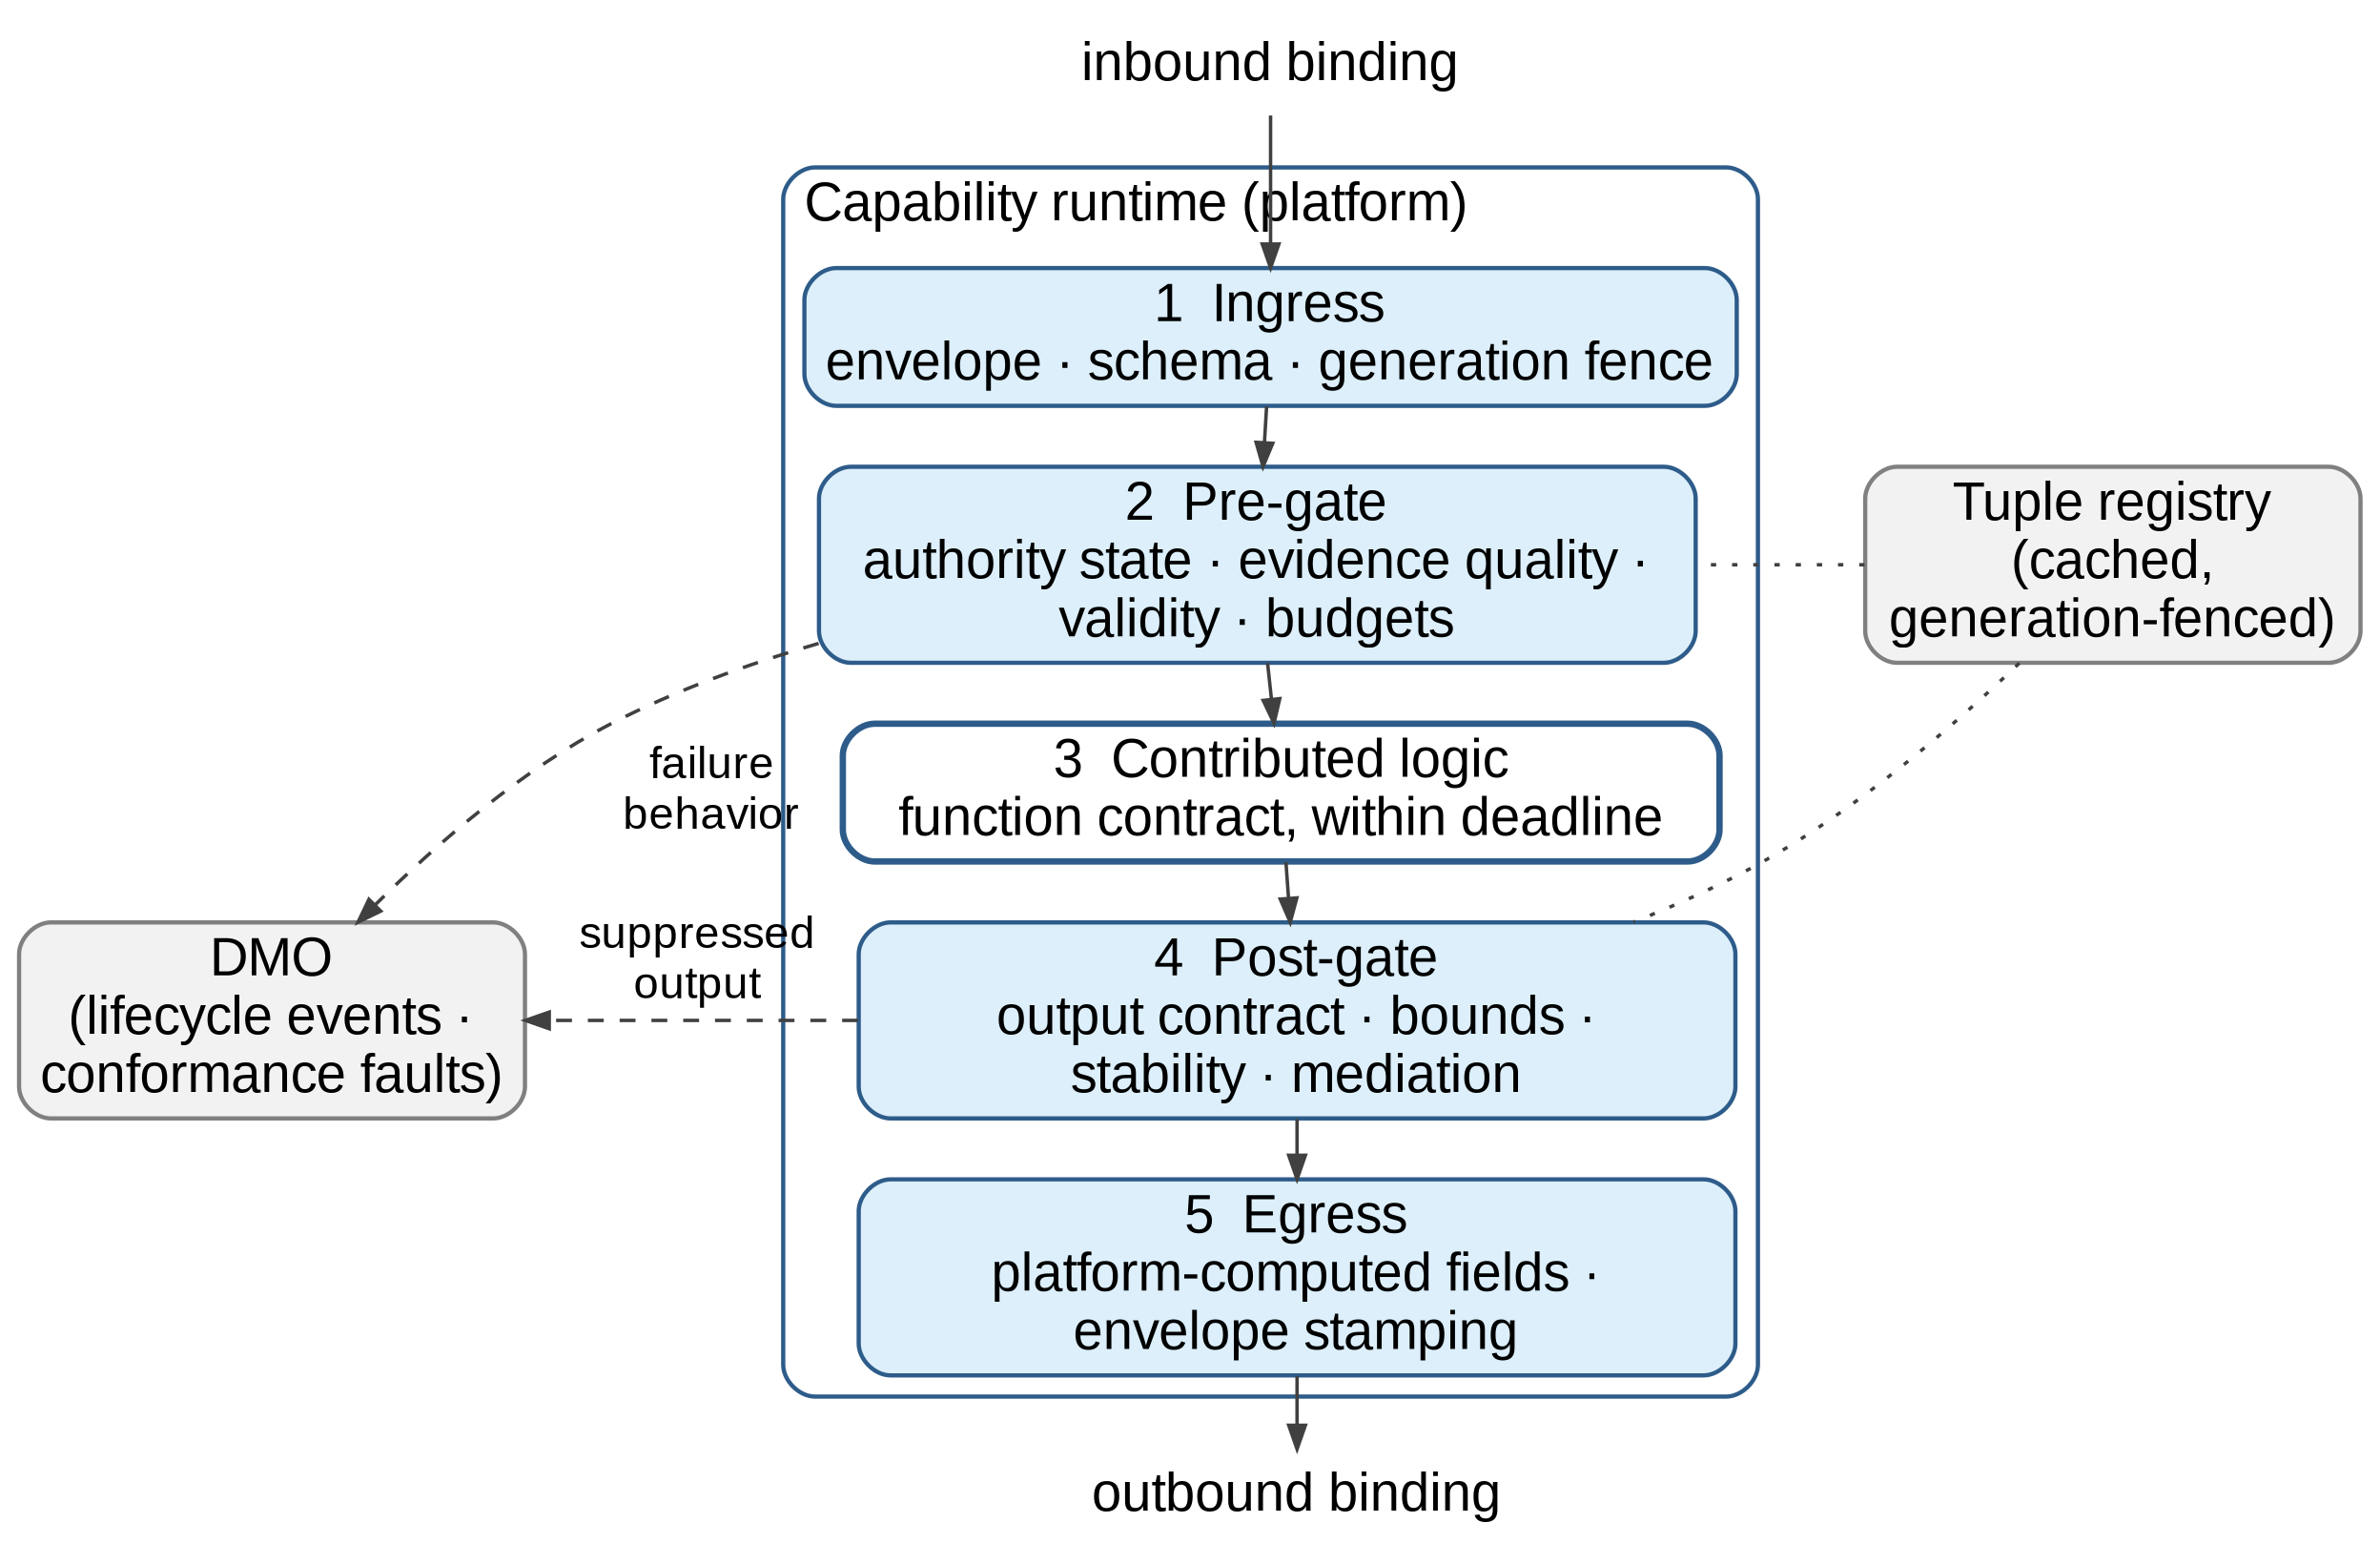
\includegraphics[width=\linewidth,height=0.45\textheight,keepaspectratio]{figures/image4.png}
\captionnum{3-4}
\caption{Execution cycle of a capability}
\label{fig:3-4}
\end{figure}

\hypertarget{function-contracts-and-cycle-order}{%
\subsubsection{Function contracts and cycle order}\label{function-contracts-and-cycle-order}}

The runtime invokes contributed logic through the function contract of
its capability (Table 3-36). A function contract is a logical signature:
it fixes what the logic receives and what it returns, not the
programming language or the transport between runtime and logic.

\begin{wptable}{3-36}

\begin{longtable}[]{@{}
  >{\raggedright\arraybackslash}p{(\columnwidth - 8\tabcolsep) * \real{0.1312}}
  >{\raggedright\arraybackslash}p{(\columnwidth - 8\tabcolsep) * \real{0.1875}}
  >{\raggedright\arraybackslash}p{(\columnwidth - 8\tabcolsep) * \real{0.1312}}
  >{\raggedright\arraybackslash}p{(\columnwidth - 8\tabcolsep) * \real{0.2875}}
  >{\raggedright\arraybackslash}p{(\columnwidth - 8\tabcolsep) * \real{0.2625}}@{}}
\caption{Function contracts of contributed logic}\tabularnewline
\toprule\noalign{}
\begin{minipage}[b]{\linewidth}\raggedright
\textbf{Capability}
\end{minipage} & \begin{minipage}[b]{\linewidth}\raggedright
\textbf{Trigger}
\end{minipage} & \begin{minipage}[b]{\linewidth}\raggedright
\textbf{Function}
\end{minipage} & \begin{minipage}[b]{\linewidth}\raggedright
\textbf{Receives from the runtime}
\end{minipage} & \begin{minipage}[b]{\linewidth}\raggedright
\textbf{Returns}
\end{minipage} \\
\midrule\noalign{}
\endfirsthead
\toprule\noalign{}
\begin{minipage}[b]{\linewidth}\raggedright
\textbf{Capability}
\end{minipage} & \begin{minipage}[b]{\linewidth}\raggedright
\textbf{Trigger}
\end{minipage} & \begin{minipage}[b]{\linewidth}\raggedright
\textbf{Function}
\end{minipage} & \begin{minipage}[b]{\linewidth}\raggedright
\textbf{Receives from the runtime}
\end{minipage} & \begin{minipage}[b]{\linewidth}\raggedright
\textbf{Returns}
\end{minipage} \\
\midrule\noalign{}
\endhead
\bottomrule\noalign{}
\endlastfoot
\textbf{MS} & Periodic, a source event, a schedule, or a request &
collect & Window; scope view of the granted identifiers; declared
sources, read-only & Measurement records: object, metric, value, unit,
event time, sample quality \\
\textbf{AE} & Input arrival with batching window, periodic, a schedule,
or a request & analyze & Consumed observations or data products;
features; context & Insights: insight type, payload, model confidence,
subject scope, validity window \\
\textbf{DE} & Insight arrival, periodic or a schedule; outcomes, verdict
expiries and notifications & decide & Insights, or observations where
the AE is none; objective status; state of the controlled objects; view
of the action space and bounds; live grants & NO\_\allowbreak{}ACTION,
or intent proposals: action type, targets, parameters, validity window,
urgency, decision confidence, rationale \\
\textbf{ACT} & Intent arrival & translate & Mediated intent; state of
the target & Controller commands; the function is deterministic and has
no side effects \\
\end{longtable}

\end{wptable}

The runtime executes the cycle of each capability in the order below. A
step that fails ends the cycle with the consequence stated, and the
failure is reported to the DMO as a lifecycle or conformance event.

The Monitoring System cycle:

\begin{enumerate}
\def\labelenumi{\arabic{enumi}.}
\tightlist
\item
  Supply the window and the scope view, which consists of the concrete
  identifiers of the observation scope granted to the instance.
\item
  Invoke \texttt{collect} within its deadline.
\item
  Discard every record outside the scope view, recording each as a
  conformance fault, and validate metric identifiers and units against
  the observation contract.
\item
  Compute \texttt{scope\_\allowbreak{}coverage} from the scope view and the
  identifiers present, and mark records older than the staleness
  threshold as stale.
\item
  Stamp the envelope and publish, pseudonymizing scope-tag values that
  identify a tenant or a slice where the binding crosses a trust
  boundary.
\end{enumerate}

The Analytics Engine cycle:

\begin{enumerate}
\def\labelenumi{\arabic{enumi}.}
\tightlist
\item
  Assemble the inputs from the observation envelopes or data products
  received for the trigger.
\item
  Compute \texttt{input\_\allowbreak{}quality} from the coverage and timestamps of
  the inputs. Where coverage is below the declared minimum or staleness
  exceeds the declared maximum, execute the declared input behavior
  without invoking the logic.
\item
  Evaluate the validity conditions over the input features and set
  \texttt{validity\_\allowbreak{}state}. Where the state is
  out\_\allowbreak{}of\_\allowbreak{}envelope and the declared behavior
  is insight\_\allowbreak{}unavailable, emit it without invoking the
  logic.
\item
  Invoke \texttt{analyze} within its deadline.
\item
  Check each returned insight against the declared insight types and
  their schemas, and reject any actuation-shaped content.
\item
  Attach \texttt{input\_\allowbreak{}quality}, \texttt{validity\_\allowbreak{}state} and the
  model's provenance, record the inference latency, stamp the envelope
  and publish.
\end{enumerate}

The Decision Engine cycle, executed one cycle at a time per agent
instance:

\begin{enumerate}
\def\labelenumi{\arabic{enumi}.}
\tightlist
\item
  Read the authority state. In
  admitted\_\allowbreak{}not\_\allowbreak{}active,
  monitoring\_\allowbreak{}only and suspended the logic is not invoked;
  in advisory, outputs are routed as recommendations at step 10.
\item
  Check the re-decision budget of each objective. Where it is exhausted,
  raise an objective-unachievable event and do not invoke the logic for
  that objective.
\item
  Evaluate the evidence. Where any consumed input has
  \texttt{degraded\_\allowbreak{}input} set or coverage below the declared minimum,
  execute the declared degraded-evidence behavior; where no usable
  insight is available, execute the declared insight-unavailable
  behavior. In either case the logic is not invoked.
\item
  Invoke \texttt{decide} within its deadline.
\item
  For each proposal whose decision confidence is below the declared
  threshold, execute the declared low-confidence behavior.
\item
  Check each proposal against its contract: the intent schema; the
  action type within the action space and any declared decision-space
  restriction; the parameters within their bounds as narrowed by the
  granted authority and the authority state; the targets within the
  granted control scope; and a complete rationale. A proposal that fails
  is dropped and recorded as a conformance fault.
\item
  Apply the stability controls and rate limit of the action type. A
  proposal that violates them is suppressed and recorded as a
  conformance fault.
\item
  Mediate. A proposal within a live action envelope grant proceeds with
  the grant reference; a proposal for which a held distributed policy
  evaluates as satisfied proceeds with the policy evaluation record;
  every other proposal is submitted to the conflict fabric, and the
  cycle waits for the verdict.
\item
  Apply the verdict. On allow, the proposal proceeds. On modify, the
  proposal is replaced by the returned bounded alternative --- a bounded
  approval being a modify whose alternative is the proposal clamped to
  the returned bounds --- which is re-checked at steps 6 and 7 and
  treated as deny if it fails. The bounds of a verdict apply to the
  proposal submitted and are not retained for later proposals. On defer,
  the proposal is held until its retry-after time, at which the cycle
  resumes from step 1. Deny, and a mediation timeout, execute the
  declared conflict-unresolved behavior.
\item
  Assign the correlation identifier, stamp the envelope with the
  mediation reference and emit the intent to the ACT, or publish it as a
  recommendation in the advisory state.
\end{enumerate}

The Actuator transaction, executed one transaction at a time per target
of an agent instance:

\begin{enumerate}
\def\labelenumi{\arabic{enumi}.}
\tightlist
\item
  Validate the intent's envelope and generation, and the presence and
  liveness of its mediation reference.
\item
  Re-validate the intent against the registry: action space, granted
  control scope, the bounds and expiry of the live grant, and the
  authority state.
\item
  Apply the rate limit and the per-target serialization.
\item
  Evaluate the declared preconditions against the state of the target.
\item
  Invoke \texttt{translate} within its deadline, and check that every
  returned command is a controller operation that the catalog maps to
  the intent's action type.
\item
  Submit the commands through the southbound adapter and wait for at
  most the actuation timeout.
\item
  Classify the response: an explicit refusal is REJECTED; a timeout or a
  loss of transport is UNRESOLVED; an acknowledgement proceeds to
  verification.
\item
  Verify. In-band verification reads back the state through the declared
  method and yields ACKNOWLEDGED\_\allowbreak{}VERIFIED on a match and
  ACKNOWLEDGED\_\allowbreak{}UNVERIFIED otherwise. Deferred verification
  publishes ACKNOWLEDGED\_\allowbreak{}UNVERIFIED marked provisional and
  publishes the final outcome when verification completes or its
  deadline expires.
\item
  Apply the retry matrix and the rollback rules of the declared failure
  policy (Chapter 7).
\item
  Publish the outcome to the DE and to the DMO, and close the
  correlation.
\end{enumerate}

A failure of \texttt{translate}, whether an error or an overrun, ends
the transaction as REJECTED with the reason code
TRANSLATION\_\allowbreak{}FAILED: nothing was submitted, and the state
of the target is known.

\hypertarget{deadlines}{%
\subsubsection{Deadlines}\label{deadlines}}

Each invocation of contributed logic has a deadline. The declared
latency of a capability --- its 99th-percentile latency
\emph{d}\textsubscript{i}, declared in \texttt{operations.latency\_\allowbreak{}p99}
--- is the minimum the capability requires to complete its work, not a
claim on the loop budget.

The time actuation needs is provided for before any slack exists. The
effective loop latency L (Section 3.8.3) contains the declared latency
of the ACT and the mediation and verification terms of its action types
(Table 3-38), so the slack S = B − L of an agent with effective budget B
is what remains once actuation is provided for. The slack is shared
between the capabilities of the loop in proportion to their declared
latencies: the deadline of capability \emph{i} is
\emph{d}\textsubscript{i} + S·\emph{d}\textsubscript{i} /
Σ\emph{d}\textsubscript{j}, so that the deadlines of one loop, together
with its transport, platform overhead, mediation and verification terms,
sum to its budget. No deadline is less than the declared latency of its
capability, and the deadline of the ACT is never reduced to make room
for a capability that precedes it.

The share of slack in a deadline is a tolerance against variation, not
an allowance. The runtime measures each capability against its declared
latency, and a capability whose measured 99th-percentile latency exceeds
it is in breach of its declaration, which Section 3.8.3 resolves by
replacing declared latencies with measured ones and, on a sustained
breach, re-stamping the effective class. An analytics step that runs
slower than planned therefore consumes its own tolerance and never the
time provided for actuation.

Where L exceeds the declared budget, no slack remains and the budget
cannot provide for actuation. The agent is then not admitted at its
declared latency class, and Section 3.8.3 determines whether it is
admitted at a lower class or rejected: an agent is never admitted with a
deadline its actuation cannot meet. For the offline class, the deadline
of each invocation is its declared latency.

An invocation that exceeds its deadline is abandoned by the runtime and
treated as an error of the logic: the MS publishes a gap for the window,
the AE emits insight\_\allowbreak{}unavailable, the DE emits no intent
for the cycle, and the ACT ends the transaction with
TRANSLATION\_\allowbreak{}FAILED.\allowbreak{}

\hypertarget{state-isolation-and-sharing}{%
\subsubsection{State, isolation and sharing}\label{state-isolation-and-sharing}}

Contributed logic may hold state. That state is private to one
capability of one agent instance and is keyed by agentInstanceId. Where
the physical deployment declares a capability stateful, its state is
persisted in the state store provided by the DMO; where it declares the
state retained, the state is restored into each new generation;
otherwise a new generation starts with empty state.

The runtime's own safety state --- re-decision budgets, retry counters,
rate-limit windows, cooldown and reversal timers, and the table of open
correlations --- is held in the state store and survives every restart,
migration and generation change. A new generation inherits it:
restarting an agent never resets a limit the agent has reached.

No state is shared between agent instances. A read-only MS collector may
serve several instances only where the service trees of the instances it
serves declare the collection service
shared\_\allowbreak{}read\_\allowbreak{}only (Table 3-31), and it then
publishes a separately scoped logical stream for each instance.

\hypertarget{time-base}{%
\subsubsection{Time base}\label{time-base}}

Every observation carries the event time at its source and the ingest
time at the MS runtime. Where a source supplies no event time, the
runtime stamps the acquisition time and marks the event time as
acquisition-derived. Timestamps are expressed in RFC 3339 UTC with
microsecond precision. The clocks of the components of one loop shall be
synchronized to within 100 µs in the real-time class, 1 ms in the
near-real-time class and 10 ms in the non-real-time class, so that loop
time, reconfiguration time and staleness are measured on a common time
base.

\hypertarget{latency-classes-and-loop-budgets}{%
\subsection{Latency Classes and Loop Budgets}\label{latency-classes-and-loop-budgets}}

\hypertarget{the-latency-classes}{%
\subsubsection{The latency classes}\label{the-latency-classes}}

The latency classes of the framework are the control-loop timescales of
the Open RAN architecture, adopted unchanged, with an offline class
added for loops that evaluate, predict or plan without acting (Table
3-37). Because the boundaries are those of the standard, a class has the
same meaning in every domain: a transport, orchestration or
non-terrestrial loop is placed by its timescale into the same classes as
a radio loop, and each class corresponds to a tier of deployed
infrastructure with known timing. The real-time class carries the
project's tightest commitments, KPI\#4, KPI\#5 and KPI\#34. Open
implementations of applications hosted at the distributed unit have been
measured closing control loops in under 450 µs on average, so the class
is reachable with a wide margin.

\begin{wptable}{3-37}

\begin{longtable}[]{@{}
  >{\raggedright\arraybackslash}p{(\columnwidth - 6\tabcolsep) * \real{0.1625}}
  >{\raggedright\arraybackslash}p{(\columnwidth - 6\tabcolsep) * \real{0.1562}}
  >{\raggedright\arraybackslash}p{(\columnwidth - 6\tabcolsep) * \real{0.2813}}
  >{\raggedright\arraybackslash}p{(\columnwidth - 6\tabcolsep) * \real{0.4000}}@{}}
\caption{Latency classes}\tabularnewline
\toprule\noalign{}
\begin{minipage}[b]{\linewidth}\raggedright
\textbf{Class}
\end{minipage} & \begin{minipage}[b]{\linewidth}\raggedright
\textbf{Loop budget B}
\end{minipage} & \begin{minipage}[b]{\linewidth}\raggedright
\textbf{Infrastructure tier}
\end{minipage} & \begin{minipage}[b]{\linewidth}\raggedright
\textbf{Conditions and concessions}
\end{minipage} \\
\midrule\noalign{}
\endfirsthead
\toprule\noalign{}
\begin{minipage}[b]{\linewidth}\raggedright
\textbf{Class}
\end{minipage} & \begin{minipage}[b]{\linewidth}\raggedright
\textbf{Loop budget B}
\end{minipage} & \begin{minipage}[b]{\linewidth}\raggedright
\textbf{Infrastructure tier}
\end{minipage} & \begin{minipage}[b]{\linewidth}\raggedright
\textbf{Conditions and concessions}
\end{minipage} \\
\midrule\noalign{}
\endhead
\bottomrule\noalign{}
\endlastfoot
\textbf{real\_\allowbreak{}time} & B \textless{} 10 ms & Applications at
the distributed and central units and at access points, beside the data
they act on & Every flow within a declared latency bound, the bounds
together within B --- LOCAL\_\allowbreak{}RUNTIME presumed, any other
binding class on evidence at admission; every action type on the
envelope or policy path; deferred verification; only local constant-time
guardrails on the per-message path \\
\textbf{near\_\allowbreak{}real\_\allowbreak{}time} & 10 ms ≤ B
\textless{} 1 s & Near-RT RIC applications; transport loops responding
to link events & Action envelopes permitted; verification in band by
default, deferred only for action types whose read-back is slow \\
\textbf{non\_\allowbreak{}real\_\allowbreak{}time} & B ≥ 1 s & Non-RT
RIC and service management and orchestration; IDMO and DMO loops;
planned transport path changes; global agents & Every intent mediated in
band unless covered by a standing grant; every actuation verified in
band \\
\textbf{offline} & No budget & Evaluation, prediction and planning
without acting & Composition classes observation, analytics and
open\_\allowbreak{}loop only; no actuation authority \\
\end{longtable}

\end{wptable}

\hypertarget{loop-time-and-reconfiguration-time}{%
\subsubsection{Loop time and reconfiguration time}\label{loop-time-and-reconfiguration-time}}

\emph{Loop time} is the time from the event time of the earliest
observation that contributed to a decision to the enforcement of the
resulting action at the managed object. \emph{Reconfiguration time} is
the time from the emission of the intent to the same enforcement.
Enforcement is established by verification: its time is the application
time reported in the read-back evidence or, where the managed object
reports none, the time of the controller's acknowledgement of the change
that verification confirmed. A cycle whose outcome is not
ACKNOWLEDGED\_\allowbreak{}VERIFIED has no established enforcement time;
it is excluded from the statistics of loop time and reconfiguration time
and counted separately. KPI\#4 and KPI\#5 are measured as
reconfiguration time, and KPI\#34 as loop time.

\hypertarget{effective-latency-and-class-assignment}{%
\subsubsection{Effective latency and class assignment}\label{effective-latency-and-class-assignment}}

Every agent declares a latency class, a loop budget within the range of
that class, the 99th-percentile latency of each of its capabilities, and
a class policy. At admission the platform computes the effective loop
latency L for the placement proposed by the DMO as the sum of the terms
of Table 3-38. The mediation and verification terms depend on the action
type, so the sum is computed for each action type of the action space
and L is the largest result.

\begin{wptable}{3-38}

\begin{longtable}[]{@{}
  >{\raggedright\arraybackslash}p{(\columnwidth - 2\tabcolsep) * \real{0.1875}}
  >{\raggedright\arraybackslash}p{(\columnwidth - 2\tabcolsep) * \real{0.8125}}@{}}
\caption{Terms of the effective loop latency}\tabularnewline
\toprule\noalign{}
\begin{minipage}[b]{\linewidth}\raggedright
\textbf{Term}
\end{minipage} & \begin{minipage}[b]{\linewidth}\raggedright
\textbf{Value used at admission}
\end{minipage} \\
\midrule\noalign{}
\endfirsthead
\toprule\noalign{}
\begin{minipage}[b]{\linewidth}\raggedright
\textbf{Term}
\end{minipage} & \begin{minipage}[b]{\linewidth}\raggedright
\textbf{Value used at admission}
\end{minipage} \\
\midrule\noalign{}
\endhead
\bottomrule\noalign{}
\endlastfoot
\textbf{Capability latency} & Declared 99th-percentile latency of each
capability (operations.\allowbreak{}latency\_\allowbreak{}p99); for a
delegated capability, the provider\textquotesingle s declared figure. \\
\textbf{Transport} & 99th-percentile latency of each binding between the
capabilities, for its binding class and the placement pair, as published
by the DMO; for LOCAL\_\allowbreak{}RUNTIME within one host, the
runtime\textquotesingle s published figure. \\
\textbf{Platform overhead} & Declared per-cycle overhead of the
capability runtimes, which shall not exceed 5\% of B at the 99th
percentile, nor 0.5 ms in the real-time class. \\
\textbf{Mediation} & Zero for an action type on the envelope or policy
path. Otherwise, the fabric\textquotesingle s measured 99th-percentile
verdict latency for the mediation mode the action requires ---
intra-domain, cross-domain or orchestrator-level --- or, where no
measurement exists, the fabric\textquotesingle s declared timeout for
that mode. \\
\textbf{Verification} & 99th-percentile latency of the declared
verification method for an action type verified in band; zero for
deferred verification. \\
\end{longtable}

\end{wptable}

The platform then assigns the effective class:

\begin{enumerate}
\def\labelenumi{\arabic{enumi}.}
\tightlist
\item
  If L does not exceed the declared budget B, the effective class is the
  declared class and the effective budget is B.
\item
  Otherwise the DMO evaluates the placements available to it that would
  sustain the declared class --- co-locating capabilities, or placing
  inference on more capable compute --- and uses one where it exists,
  and the computation is repeated for that placement.
\item
  If no such placement exists and the class policy is
  accept\_\allowbreak{}lower, the effective class is the class whose
  range contains L, the effective budget is L, and the lowering is
  recorded as a warning in the resolved configuration.
\item
  If no such placement exists and the class policy is
  reject\_\allowbreak{}if\_\allowbreak{}unmet, admission rejects the
  agent.
\end{enumerate}

The effective class, not the declared one, governs composition,
deadlines and the commitments the platform makes. At runtime, measured
latencies replace declared ones, and a sustained breach re-stamps the
effective class downward (Chapter 12).

An agent holds the real-time class only if every flow of its loop meets
a latency bound within the loop budget, every action type of its action
space is on the envelope or policy path, and the verification of every
action type is deferred with a declared deadline. A
LOCAL\_\allowbreak{}RUNTIME binding is presumed to meet the bound and is
declared without further evidence. Any other binding class is admissible
on a flow of a real-time loop where the descriptor declares the bound
the flow achieves and admission is supplied with evidence for it --- a
measurement on the proposed placement, or a commitment of the transport
that carries the flow --- sufficient for the sum of the bounds of the
loop's flows to lie within the loop budget. The class is a property of
the latency the loop achieves, not of the placement by which it achieves
it; a flow admitted on declared evidence is subject to the same runtime
re-stamping as any other. An intent of a real-time agent that falls
outside its live action envelope remains permitted: it is submitted for
mediation, and its cycle is recorded as outside the class commitment.

\hypertarget{non-terrestrial-segments}{%
\subsubsection{Non-terrestrial segments}\label{non-terrestrial-segments}}

Propagation over a non-terrestrial segment is a property of distance and
cannot be reduced by resources. A loop whose path crosses a
non-terrestrial segment shall not hold the real-time class. The
project's relaxation of its control-loop commitment by an order of
magnitude for non-terrestrial deployments (KPI\#34) corresponds to a
loop budget of 100 ms, which lies in the near-real-time class. Because
the transport terms of the effective latency are computed from the
actual placement, a capability placed across such a segment from the
rest of its loop is visible at admission and cannot take part in a loop
faster than the segment allows.

\hypertarget{authority-and-bounds}{%
\subsection{Authority and Bounds}\label{authority-and-bounds}}

\hypertarget{the-bound-stack}{%
\subsubsection{The bound stack}\label{the-bound-stack}}

An action of an agent is permitted if, and only if, it lies within every
one of the five bounds of Table 3-39. Each bound is set by a different
party and held by the platform, never by the agent. A bound may narrow
what the bounds before it permit; none may widen it. In particular,
neither a modify verdict nor an action envelope can authorize an action
outside the declared contract or the granted authority, and no authority
state restores scope that was withheld at admission.

\begin{wptable}{3-39}

\begin{longtable}[]{@{}
  >{\raggedright\arraybackslash}p{(\columnwidth - 8\tabcolsep) * \real{0.1750}}
  >{\raggedright\arraybackslash}p{(\columnwidth - 8\tabcolsep) * \real{0.3000}}
  >{\raggedright\arraybackslash}p{(\columnwidth - 8\tabcolsep) * \real{0.1813}}
  >{\raggedright\arraybackslash}p{(\columnwidth - 8\tabcolsep) * \real{0.1438}}
  >{\raggedright\arraybackslash}p{(\columnwidth - 8\tabcolsep) * \real{0.2000}}@{}}
\caption{The bound stack}\tabularnewline
\toprule\noalign{}
\begin{minipage}[b]{\linewidth}\raggedright
\textbf{Bound}
\end{minipage} & \begin{minipage}[b]{\linewidth}\raggedright
\textbf{Content}
\end{minipage} & \begin{minipage}[b]{\linewidth}\raggedright
\textbf{Set by}
\end{minipage} & \begin{minipage}[b]{\linewidth}\raggedright
\textbf{Held in}
\end{minipage} & \begin{minipage}[b]{\linewidth}\raggedright
\textbf{Checked at}
\end{minipage} \\
\midrule\noalign{}
\endfirsthead
\toprule\noalign{}
\begin{minipage}[b]{\linewidth}\raggedright
\textbf{Bound}
\end{minipage} & \begin{minipage}[b]{\linewidth}\raggedright
\textbf{Content}
\end{minipage} & \begin{minipage}[b]{\linewidth}\raggedright
\textbf{Set by}
\end{minipage} & \begin{minipage}[b]{\linewidth}\raggedright
\textbf{Held in}
\end{minipage} & \begin{minipage}[b]{\linewidth}\raggedright
\textbf{Checked at}
\end{minipage} \\
\midrule\noalign{}
\endhead
\bottomrule\noalign{}
\endlastfoot
\textbf{1. Declared contract} & Action space with bounds, rate limits
and stability controls; observation and control scope & Contributor, in
the descriptor & Registry, from admission & Admission; DE post-gate; ACT
last-mile check \\
\textbf{2. Granted authority} & Granted control scope, narrowed bounds,
priority band, authority ceiling; for a delegation, the authority
envelope & IDMO and DMO, at admission or in the delegation & Registry &
Admission; DE post-gate; ACT last-mile check \\
\textbf{3. Authority state} & One of the seven states of Table 3-12 &
DMO or IDMO: activation gate, evaluation, lifecycle & Registry & DE
pre-gate, every cycle; ACT last-mile check \\
\textbf{4. Mediation} & Verdict, action envelope grant or distributed
policy & Conflict fabric & Registry for grants; message for verdict
references & DE post-gate; ACT last-mile check against the live grant \\
\textbf{5. Class and KPI bounds} & Effective latency class and budget;
bounds derived from project KPIs & Admission, from the class definitions
and project KPIs & Registry & Admission; runtime measurement \\
\end{longtable}

\end{wptable}

\hypertarget{envelopes-of-authority}{%
\subsubsection{Envelopes of authority}\label{envelopes-of-authority}}

Three mechanisms pre-authorize action so that it can proceed without a
round trip, and all three have the same shape: a bounded region of
permitted action, with a validity window, inside which action proceeds
and outside which approval is required. The \emph{action envelope} is
granted by the conflict fabric over a region of an agent's action space,
and is what makes the real-time class compatible with mediation. The
\emph{authority envelope} is granted by the IDMO to a DMO in a
delegation, and is what makes hierarchy compatible with local latency.
The \emph{distributed policy} is granted by the fabric on request, and
lets an agent establish conflict-freedom locally where the region cannot
be enumerated in advance. In each case authority originates with the
granting party, and the agent acts only within authority already
granted; an agent never authorizes itself.

A grant is void when its validity expires, when the granting party
withdraws it, and when the agent's underlying domain service is migrated
or terminated by orchestration. Voiding takes effect at the next
last-mile check of the ACT, which checks every command against the live
grant rather than a cached copy.

\hypertarget{bounds-derived-from-kpis}{%
\subsubsection{Bounds derived from KPIs}\label{bounds-derived-from-kpis}}

The bounds of the latency classes and of the platform's own overhead are
derived from the project KPIs: the real-time class from KPI\#4, KPI\#5
and KPI\#34, and the per-cycle overhead of the guardrails --- at most
5\% of the loop budget at the 99th percentile, and 0.5 ms in the
real-time class --- from the same commitments. An agent whose
declaration cannot meet the bounds of the class it requests is assigned
a class it can sustain, or rejected, at admission (Section 3.8.3); an
agent whose measured behavior leaves those bounds during operation is
re-classed or demoted. Chapter 12 derives the full set of bounds from
the project KPIs and states for each whether an agent outside it is
re-classed, demoted or rejected.

\hypertarget{coexistence-with-conventionally-managed-services}{%
\subsection{Coexistence with Conventionally Managed Services}\label{coexistence-with-conventionally-managed-services}}

The architecture accommodates several ways of realizing a managed
service, and services defined conventionally, without tuples, coexist
with agent-managed services in the same deployment. The following rules
govern the boundary between them.

\begin{itemize}
\tightlist
\item
  A domain in which no agent is instantiated is managed without one. No
  tuple artifact is instantiated there, and nothing in this framework
  applies to the services in that domain.
\item
  Agent instantiation is independent of service orchestration, so one
  end-to-end service may span agent-managed domains and conventionally
  managed ones.
\item
  An automated control function outside the framework, such as a legacy
  optimization function or a loop internal to a controller, that acts on
  control parameters in a domain where agents hold control scope shall
  either take part in conflict mediation, submitting its actions as an
  agent does, or have the control parameters it acts on reserved. A
  reserved parameter is registered with the conflict fabric as held by
  an external controller and shall not be granted to the control scope
  of any agent. The DMO applies this rule when it grants control scope.
\item
  A manual intervention by an operator on control parameters within an
  agent's granted control scope takes precedence over the agent. The DMO
  withdraws those parameters from the agent's granted control scope from
  the moment of the intervention and holds them withdrawn until control
  over them is explicitly returned. The hold does not expire, and no
  elapsed interval, restored objective or later agent proposal ends it:
  a human decision stands until a human reverses it. A held parameter is
  registered with the conflict fabric as held, and the DMO raises a
  standing assurance signal, from the moment of the hold until its
  return, naming the parameter, the agent whose scope it left and the
  time the hold began, so that a hold left in place is visible to
  operations rather than silent. The agent continues to operate on the
  remainder of its granted control scope where its descriptor declares
  objectives that remain achievable without the held parameter; where it
  does not, the agent enters the degraded operation its failure policy
  declares, and the cause recorded is the hold and not a fault of the
  agent. Any action envelope held against a withdrawn parameter is
  voided. A recommendation of an open-loop agent that an operator
  applies is such an intervention.
\item
  A lifecycle operation of the orchestration layer on an agent's
  underlying domain service --- migration, scaling or termination --- is
  a lifecycle event for the agent: the generation is incremented,
  decision authority is suspended from the moment the operation begins,
  and any action envelope held against the affected scope is voided
  (Chapter 9).
\item
  Observation confers no control. An agent may observe conventionally
  managed resources within its observation scope, and its control scope
  contains only what admission grants.
\end{itemize}

\hypertarget{requirements}{%
\subsection{Requirements}\label{requirements}}

The requirements of the agentic framework that are not specific to one
capability are listed in the tables below.

\begin{requirement}{Req-T23-FW-01}{MUST}{Tuple composition}
\reqfield{Description / rationale}{%
Every agent shall be composed of the four capabilities MS, AE, DE and
ACT, each declared in its descriptor in exactly one capability mode:
full, partial, delegated or none. The platform shall derive the
agent\textquotesingle s composition class from the declared modes, and
the class shall bound the highest authority state the agent can hold. A
descriptor whose modes fit no composition class shall be invalid.}
\reqfield{Dependency}{%
None}
\reqfield{Traceability (Forward)}{%
\begin{itemize}
\item
  Checked by the validity rules before admission.
\item
  Composition class recorded in the registry and reported in assurance.
\end{itemize}}
\reqfield{UNITY-6G components}{%
\begin{itemize}
\item
  Tuple descriptor
\item
  Tuple registry and admission (IDMO/DMO)
\end{itemize}}
\reqfield{Linked KPIs}{%
\begin{itemize}
\item
  KPI\#1: Deliver four distributed management entities (MS, AE, DE and
  ACT) deployable in each heterogeneous domain.
\item
  KPI\#26: Increase the ratio of service management and LCM tasks
  resolved by local AE/DE components.
\end{itemize}}
\end{requirement}

\begin{requirement}{Req-T23-FW-02}{MUST}{Typed capability outputs}
\reqfield{Description / rationale}{%
Each capability shall produce only its own semantic object: observations
from the MS, insights from the AE, intents from the DE and outcomes from
the ACT. A contract whose schema carries content of another
capability\textquotesingle s output --- model outputs in an observation,
actuation-shaped fields in an insight, controller-native commands in an
intent --- shall be rejected, and an object carrying such content shall
be rejected at the binding boundary.}
\reqfield{Dependency}{%
Req-T23-FW-01}
\reqfield{Traceability (Forward)}{%
\begin{itemize}
\item
  Checked by the validity rules against the declared schemas.
\item
  Enforced at every binding boundary by the capability runtimes.
\end{itemize}}
\reqfield{UNITY-6G components}{%
\begin{itemize}
\item
  Capability runtimes
\item
  Tuple descriptor
\end{itemize}}
\reqfield{Linked KPIs}{%
\begin{itemize}
\item
  KPI\#1: Deliver four distributed management entities (MS, AE, DE and
  ACT) deployable in each heterogeneous domain.
\item
  KPI\#36: Guarantee 99.99999\% service availability and reliability
  based on effective monitoring and LCM.
\end{itemize}}
\end{requirement}

\begin{requirement}{Req-T23-FW-03}{MUST}{Capability mode obligations}
\reqfield{Description / rationale}{%
A partial capability shall enumerate its subset. A delegated capability
shall name its provider, the provider\textquotesingle s interface, a
pinned interface profile, a range of accepted provider versions and its
SLA assumptions, and admission shall verify that the
provider\textquotesingle s scope covers the consumer\textquotesingle s
and that the provider\textquotesingle s declared latency and freshness
meet those assumptions. MS and ACT delegations shall remain within the
domain; an AE delegation may cross domains as a data product or an
exposed contract; a DE delegation may cross domains only to the
agent\textquotesingle s own global agent.}
\reqfield{Dependency}{%
Req-T23-FW-01}
\reqfield{Traceability (Forward)}{%
\begin{itemize}
\item
  Checked by the validity rules and at admission.
\item
  Binding fault raised at runtime when a provider leaves the pinned
  range.
\end{itemize}}
\reqfield{UNITY-6G components}{%
\begin{itemize}
\item
  Tuple descriptor
\item
  Admission (IDMO/DMO)
\item
  Provider agents and reused capabilities
\end{itemize}}
\reqfield{Linked KPIs}{%
\begin{itemize}
\item
  KPI\#1: Deliver four distributed management entities (MS, AE, DE and
  ACT) deployable in each heterogeneous domain.
\item
  KPI\#36: Guarantee 99.99999\% service availability and reliability
  based on effective monitoring and LCM.
\end{itemize}}
\end{requirement}

\begin{requirement}{Req-T23-FW-04}{MUST}{The descriptor as the single contract}
\reqfield{Description / rationale}{%
An agent\textquotesingle s scope, objectives, action space, failure
behavior, latency class and permitted bindings shall be read only from
its admitted descriptor, from the values bound at its instantiation and
from the delegation it realizes, where it realizes one. No value
reported by an agent at runtime shall extend them, and a
platform-computed field shall never be accepted from contributed logic.}
\reqfield{Dependency}{%
None}
\reqfield{Traceability (Forward)}{%
\begin{itemize}
\item
  Enforced by admission and by the capability runtimes.
\end{itemize}}
\reqfield{UNITY-6G components}{%
\begin{itemize}
\item
  Tuple registry
\item
  Capability runtimes
\end{itemize}}
\reqfield{Linked KPIs}{%
\begin{itemize}
\item
  KPI\#33: Support more tenants via distributed AI \& DLT.
\item
  KPI\#36: Guarantee 99.99999\% service availability and reliability
  based on effective monitoring and LCM.
\end{itemize}}
\end{requirement}

\begin{requirement}{Req-T23-FW-05}{MUST}{Descriptor structure}
\reqfield{Description / rationale}{%
A descriptor shall contain the sections of Table 3-13 required for its
composition class, and no section marked absent for that class, and
shall conform to the schema version it declares. Payload schemas shall
be JSON Schema 2020-12 documents referenced by identifier and version,
and predicates shall be structured conditions of the form defined in
Table 3-3, evaluable without an expression interpreter.}
\reqfield{Dependency}{%
Req-T23-FW-01}
\reqfield{Traceability (Forward)}{%
\begin{itemize}
\item
  Validated against the JSON Schema rendering of the descriptor (Annex
  A).
\end{itemize}}
\reqfield{UNITY-6G components}{%
\begin{itemize}
\item
  Tuple descriptor
\item
  Schema registry
\end{itemize}}
\reqfield{Linked KPIs}{%
\begin{itemize}
\item
  KPI\#1: Deliver four distributed management entities (MS, AE, DE and
  ACT) deployable in each heterogeneous domain.
\item
  KPI\#46: Availability of four open-source frameworks and their
  corresponding API specifications for the UNITY-6G PoCs.
\end{itemize}}
\end{requirement}

\begin{requirement}{Req-T23-FW-06}{MUST}{Validity before admission}
\reqfield{Description / rationale}{%
A descriptor shall satisfy every validity rule of Table 3-30 before it
is submitted to admission. A failure shall be reported with the
identifier of every rule violated, and a descriptor that fails any rule
shall not be admitted.}
\reqfield{Dependency}{%
Req-T23-FW-05}
\reqfield{Traceability (Forward)}{%
\begin{itemize}
\item
  Checked by a validator that operates on the descriptor, its schemas
  and the catalog alone.
\end{itemize}}
\reqfield{UNITY-6G components}{%
\begin{itemize}
\item
  Descriptor validator
\item
  Type catalog
\end{itemize}}
\reqfield{Linked KPIs}{%
\begin{itemize}
\item
  KPI\#6: Decrease service creation and termination time.
\item
  KPI\#41: Reduction of 70\% of deployment time of AI-based
  resource/energy management algorithms.
\end{itemize}}
\end{requirement}

\begin{requirement}{Req-T23-FW-07}{MUST}{Versioning and immutability}
\reqfield{Description / rationale}{%
A descriptor shall be identified by its descriptor\_\allowbreak{}id and
a semantic version. An admitted version shall be immutable: any change
to its content, artifacts, models or parameters shall produce a new
version, admitted as a new descriptor. The registry shall record the
content hash of every admitted version, and every instance shall
reference exactly one version.}
\reqfield{Dependency}{%
Req-T23-FW-08}
\reqfield{Traceability (Forward)}{%
\begin{itemize}
\item
  Checked at admission against the registry.
\end{itemize}}
\reqfield{UNITY-6G components}{%
\begin{itemize}
\item
  Tuple registry
\item
  Type catalog
\end{itemize}}
\reqfield{Linked KPIs}{%
\begin{itemize}
\item
  KPI\#33: Support more tenants via distributed AI \& DLT.
\item
  KPI\#37: Guarantee 99.99999\% service continuity through AI-driven
  proactive management of cloud-native services.
\end{itemize}}
\end{requirement}

\begin{requirement}{Req-T23-FW-08}{MUST}{Integrity}
\reqfield{Description / rationale}{%
A descriptor shall carry a content hash over its canonical form (RFC
8785) and the signature of its publisher; every artifact shall be
referenced by digest with a software bill of materials that pins each
software dependency, and every platform service the agent requires shall
be declared with a minimum version. A descriptor whose hash or signature
does not verify against the publisher\textquotesingle s key in its trust
domain shall be rejected before any other check.}
\reqfield{Dependency}{%
None}
\reqfield{Traceability (Forward)}{%
\begin{itemize}
\item
  Verified first at admission.
\item
  Attestations checked where the trust domain requires them.
\end{itemize}}
\reqfield{UNITY-6G components}{%
\begin{itemize}
\item
  Tuple registry
\item
  Trust layer (T2.4)
\end{itemize}}
\reqfield{Linked KPIs}{%
\begin{itemize}
\item
  KPI\#33: Support more tenants via distributed AI \& DLT.
\end{itemize}}
\end{requirement}

\begin{requirement}{Req-T23-FW-09}{MUST}{Bounded extension}
\reqfield{Description / rationale}{%
Extension fields shall be named
x-\textless publisher\textgreater-\textless name\textgreater{} and shall
appear only at the top level of the descriptor, within the capability
sections of functions and within model\_\allowbreak{}hooks; they shall
not appear in scope, action\_\allowbreak{}space, policies,
failure\_\allowbreak{}policy, interfaces,
physical\_\allowbreak{}deployment, ownership or integrity. A descriptor
containing any extension field or extension type shall be of extension
conformance and shall enter at the advisory authority state.}
\reqfield{Dependency}{%
Req-T23-FW-05}
\reqfield{Traceability (Forward)}{%
\begin{itemize}
\item
  Checked by the validity rules.
\item
  Conformance class recorded in the registry.
\end{itemize}}
\reqfield{UNITY-6G components}{%
\begin{itemize}
\item
  Tuple descriptor
\item
  Admission (IDMO/DMO)
\end{itemize}}
\reqfield{Linked KPIs}{%
\begin{itemize}
\item
  KPI\#33: Support more tenants via distributed AI \& DLT.
\item
  KPI\#41: Reduction of 70\% of deployment time of AI-based
  resource/energy management algorithms.
\end{itemize}}
\end{requirement}

\begin{requirement}{Req-T23-FW-10}{MUST}{Descriptor levels}
\reqfield{Description / rationale}{%
A local agent shall be described by a LocalAINativeAgent descriptor
owned by a DMO, and a global agent by a GlobalAINativeAgent descriptor
owned by the IDMO. The IDMO shall address a domain on behalf of a global
agent only through DomainAgentDelegation documents. Neither a global
descriptor nor a delegation shall contain domain-internal placement,
deployment or controller mapping.}
\reqfield{Dependency}{%
Req-T23-FW-05}
\reqfield{Traceability (Forward)}{%
\begin{itemize}
\item
  Checked by the validity rules and at admission.
\end{itemize}}
\reqfield{UNITY-6G components}{%
\begin{itemize}
\item
  IDMO
\item
  DMO
\item
  Tuple descriptor
\end{itemize}}
\reqfield{Linked KPIs}{%
\begin{itemize}
\item
  KPI\#1: Deliver four distributed management entities (MS, AE, DE and
  ACT) deployable in each heterogeneous domain.
\item
  KPI\#18: Reduction in the deployment time of heterogeneous domain
  services.
\item
  KPI\#26: Increase the ratio of service management and LCM tasks
  resolved by local AE/DE components.
\end{itemize}}
\end{requirement}

\begin{requirement}{Req-T23-FW-11}{MUST}{Agent service tree}
\reqfield{Description / rationale}{%
An agent descriptor shall declare the service tree of its tuples,
stating for each tuple the services it requires in order to perform its
capability and the bindings that interconnect the tuples into a closed
loop. A GlobalAINativeAgent descriptor shall be issued to the IDMO and a
LocalAINativeAgent descriptor to the DMO of its domain, and the
receiving orchestrator shall instantiate the declared services and bind
them before the agent is activated. A resource-facing service shall
carry no agent content.}
\reqfield{Dependency}{%
Req-T23-FW-04}
\reqfield{Traceability (Forward)}{%
\begin{itemize}
\item
  Checked at admission of the descriptor and at instantiation.
\end{itemize}}
\reqfield{UNITY-6G components}{%
\begin{itemize}
\item
  IDMO
\item
  DMO
\end{itemize}}
\reqfield{Linked KPIs}{%
\begin{itemize}
\item
  KPI\#1: Deliver four distributed management entities (MS, AE, DE and
  ACT) deployable in each heterogeneous domain.
\item
  KPI\#6: Decrease service creation and termination time.
\item
  KPI\#18: Reduction in the deployment time of heterogeneous domain
  services.
\end{itemize}}
\end{requirement}

\begin{requirement}{Req-T23-FW-12}{MUST}{Isolation of instances}
\reqfield{Description / rationale}{%
Every agent instance shall be isolated by the triple
descriptor\_\allowbreak{}id, assignedDomainId and agentInstanceId, with
its own policy state, model state, decision history, action correlation,
evaluation windows and lifecycle. A monitoring collector shall be shared
between instances only where the service trees of the instances it
serves declare the collection service
shared\_\allowbreak{}read\_\allowbreak{}only, and shall then publish a
separately scoped logical stream for each instance.}
\reqfield{Dependency}{%
Req-T23-FW-11}
\reqfield{Traceability (Forward)}{%
\begin{itemize}
\item
  Enforced by the DMO at realization and by the capability runtimes.
\end{itemize}}
\reqfield{UNITY-6G components}{%
\begin{itemize}
\item
  DMO
\item
  Capability runtimes
\item
  State store
\end{itemize}}
\reqfield{Linked KPIs}{%
\begin{itemize}
\item
  KPI\#33: Support more tenants via distributed AI \& DLT.
\item
  KPI\#36: Guarantee 99.99999\% service availability and reliability
  based on effective monitoring and LCM.
\end{itemize}}
\end{requirement}

\begin{requirement}{Req-T23-FW-13}{MUST}{Generation fencing}
\reqfield{Description / rationale}{%
The owning DMO or IDMO shall assign each agent instance a generation,
incremented at every placement, restart, migration, model update and
binding change, and at migration or termination of the underlying domain
service. Every message shall carry its producer\textquotesingle s
generation. A receiver shall discard a message of an older generation
than its binding record, and shall refresh the record from the registry
before accepting a message of a newer one.}
\reqfield{Dependency}{%
Req-T23-FW-12}
\reqfield{Traceability (Forward)}{%
\begin{itemize}
\item
  Enforced by every receiving runtime.
\end{itemize}}
\reqfield{UNITY-6G components}{%
\begin{itemize}
\item
  DMO / IDMO
\item
  Capability runtimes
\end{itemize}}
\reqfield{Linked KPIs}{%
\begin{itemize}
\item
  KPI\#36: Guarantee 99.99999\% service availability and reliability
  based on effective monitoring and LCM.
\item
  KPI\#37: Guarantee 99.99999\% service continuity through AI-driven
  proactive management of cloud-native services.
\end{itemize}}
\end{requirement}

\begin{requirement}{Req-T23-FW-14}{MUST}{Hosted contributed logic}
\reqfield{Description / rationale}{%
Contributed logic shall execute within the capability runtime of its
capability. All binding exchanges, platform-computed fields, gates,
counters, rate limits and southbound submissions shall be performed by
the runtime. Contributed logic shall open no binding, bus session or
controller session; its only input and output beyond the runtime shall
be read-only access by an MS to its declared sources, and the declared
read-only tools of a generative DE.}
\reqfield{Dependency}{%
None}
\reqfield{Traceability (Forward)}{%
\begin{itemize}
\item
  Verified at the activation gate.
\item
  Exercised in the WP6 proofs of concept.
\end{itemize}}
\reqfield{UNITY-6G components}{%
\begin{itemize}
\item
  Capability runtimes
\item
  DMO
\end{itemize}}
\reqfield{Linked KPIs}{%
\begin{itemize}
\item
  KPI\#1: Deliver four distributed management entities (MS, AE, DE and
  ACT) deployable in each heterogeneous domain.
\item
  KPI\#36: Guarantee 99.99999\% service availability and reliability
  based on effective monitoring and LCM.
\item
  KPI\#46: Availability of four open-source frameworks and their
  corresponding API specifications for the UNITY-6G PoCs.
\end{itemize}}
\end{requirement}

\begin{requirement}{Req-T23-FW-15}{MUST}{Function contracts and deadlines}
\reqfield{Description / rationale}{%
The runtime shall invoke contributed logic only through the function
contract of its capability (Table 3-36), in the cycle order of Section
3.7.2 and within the deadline of Section 3.7.3. An overrun or an error
shall be treated as the capability\textquotesingle s declared
unavailability: a gap for the MS, insight\_\allowbreak{}unavailable for
the AE, no intent for the DE, and TRANSLATION\_\allowbreak{}FAILED for
the ACT.}
\reqfield{Dependency}{%
Req-T23-FW-14}
\reqfield{Traceability (Forward)}{%
\begin{itemize}
\item
  Enforced by the capability runtimes.
\end{itemize}}
\reqfield{UNITY-6G components}{%
\begin{itemize}
\item
  Capability runtimes
\end{itemize}}
\reqfield{Linked KPIs}{%
\begin{itemize}
\item
  KPI\#4: Real-time reconfiguration of IEEE 802.11 network domain in
  range smaller than 10 ms from taking the decision.
\item
  KPI\#5: Real-time reconfiguration of cellular network domain in the
  range smaller than 10 ms from taking the decision.
\item
  KPI\#34: Reduce Open RAN real-time control loops time scales below 10
  ms and 10x in NTN for real-time 6G.
\end{itemize}}
\end{requirement}

\begin{requirement}{Req-T23-FW-16}{MUST}{Serial decision and actuation}
\reqfield{Description / rationale}{%
The decision cycles of one agent instance shall be serial. The actuation
transactions of one agent instance on one target shall be serial;
transactions on distinct targets may run concurrently up to the declared
maximum concurrency.}
\reqfield{Dependency}{%
Req-T23-FW-15}
\reqfield{Traceability (Forward)}{%
\begin{itemize}
\item
  Enforced by the DE and ACT runtimes.
\end{itemize}}
\reqfield{UNITY-6G components}{%
\begin{itemize}
\item
  Capability runtimes
\end{itemize}}
\reqfield{Linked KPIs}{%
\begin{itemize}
\item
  KPI\#21: Reduce the performance penalty due to conflicts by 20\% by
  means of DLT, hierarchical algorithms and policy-based conflict
  resolution schemes.
\item
  KPI\#36: Guarantee 99.99999\% service availability and reliability
  based on effective monitoring and LCM.
\end{itemize}}
\end{requirement}

\begin{requirement}{Req-T23-FW-17}{MUST}{Deterministic translation}
\reqfield{Description / rationale}{%
The ACT\textquotesingle s translation of intent into controller commands
shall be deterministic and free of side effects, and every command it
returns shall be a controller operation that the catalog maps to the
intent\textquotesingle s action type. Learned, generative and
simulation-based techniques shall not be admitted as translation logic.}
\reqfield{Dependency}{%
Req-T23-FW-18}
\reqfield{Traceability (Forward)}{%
\begin{itemize}
\item
  Checked at admission from the declared technique.
\item
  Command mapping checked by the ACT runtime in every transaction.
\end{itemize}}
\reqfield{UNITY-6G components}{%
\begin{itemize}
\item
  ACT runtime
\item
  Type catalog
\end{itemize}}
\reqfield{Linked KPIs}{%
\begin{itemize}
\item
  KPI\#36: Guarantee 99.99999\% service availability and reliability
  based on effective monitoring and LCM.
\item
  KPI\#42: DT-validated AI algorithms that do not break the
  time-sensitive operation when deployed in 99\% of the outputs.
\end{itemize}}
\end{requirement}

\begin{requirement}{Req-T23-FW-18}{MUST}{Technique admissibility}
\reqfield{Description / rationale}{%
Contributed logic shall declare its technique class per capability and
shall be admitted only under the conditions of Table 3-11. A generative
DE shall hold no tool that changes network state. Adaptation that
changes model weights shall produce a new model identity and take effect
only through a generation-controlled update; adaptation by accumulated
context shall declare its retained-context bound and reset condition.}
\reqfield{Dependency}{%
None}
\reqfield{Traceability (Forward)}{%
\begin{itemize}
\item
  Checked at admission.
\item
  Model identity checked at the activation gate.
\end{itemize}}
\reqfield{UNITY-6G components}{%
\begin{itemize}
\item
  Admission (IDMO/DMO)
\item
  AI/ML domain
\end{itemize}}
\reqfield{Linked KPIs}{%
\begin{itemize}
\item
  KPI\#41: Reduction of 70\% of deployment time of AI-based
  resource/energy management algorithms.
\item
  KPI\#42: DT-validated AI algorithms that do not break the
  time-sensitive operation when deployed in 99\% of the outputs.
\end{itemize}}
\end{requirement}

\begin{requirement}{Req-T23-FW-19}{MUST}{Latency class declaration}
\reqfield{Description / rationale}{%
Every agent shall declare an operating mode consistent with its
triggers, a latency class, a loop budget within the range of the class,
the 99th-percentile latency of each capability, and a class policy. An
offline agent shall hold no actuation authority.}
\reqfield{Dependency}{%
None}
\reqfield{Traceability (Forward)}{%
\begin{itemize}
\item
  Checked by the validity rules.
\end{itemize}}
\reqfield{UNITY-6G components}{%
\begin{itemize}
\item
  Tuple descriptor
\end{itemize}}
\reqfield{Linked KPIs}{%
\begin{itemize}
\item
  KPI\#4: Real-time reconfiguration of IEEE 802.11 network domain in
  range smaller than 10 ms from taking the decision.
\item
  KPI\#5: Real-time reconfiguration of cellular network domain in the
  range smaller than 10 ms from taking the decision.
\item
  KPI\#34: Reduce Open RAN real-time control loops time scales below 10
  ms and 10x in NTN for real-time 6G.
\end{itemize}}
\end{requirement}

\begin{requirement}{Req-T23-FW-20}{MUST}{Effective latency class}
\reqfield{Description / rationale}{%
Admission shall compute the effective loop latency for the proposed
placement as the sum of the terms of Table 3-38 for each action type,
taking the largest result, and shall assign the effective class by the
procedure of Section 3.8.3, using an alternative placement that sustains
the declared class, where one exists, before lowering the class or
rejecting the agent. The effective class shall govern composition,
deadlines and the platform\textquotesingle s commitments.}
\reqfield{Dependency}{%
Req-T23-FW-19}
\reqfield{Traceability (Forward)}{%
\begin{itemize}
\item
  Computed at admission; recorded in the registry and the resolved
  configuration.
\item
  Re-stamped from measured latencies at runtime.
\end{itemize}}
\reqfield{UNITY-6G components}{%
\begin{itemize}
\item
  Admission (IDMO/DMO)
\item
  DMO (placement)
\end{itemize}}
\reqfield{Linked KPIs}{%
\begin{itemize}
\item
  KPI\#4: Real-time reconfiguration of IEEE 802.11 network domain in
  range smaller than 10 ms from taking the decision.
\item
  KPI\#5: Real-time reconfiguration of cellular network domain in the
  range smaller than 10 ms from taking the decision.
\item
  KPI\#7: Cross-domain (cellular -- IEEE 802.11) end-to-end latency
  smaller than 20 ms.
\item
  KPI\#34: Reduce Open RAN real-time control loops time scales below 10
  ms and 10x in NTN for real-time 6G.
\end{itemize}}
\end{requirement}

\begin{requirement}{Req-T23-FW-21}{MUST}{Real-time class conditions}
\reqfield{Description / rationale}{%
An agent shall hold the real-time class only if every flow of its loop
meets a declared latency bound, the bounds of the loop\textquotesingle s
flows together lie within the loop budget, every action type is on the
envelope or policy path, and the verification of every action type is
deferred with a declared deadline. A LOCAL\_\allowbreak{}RUNTIME binding
shall be presumed to meet its bound; any other binding class shall be
admitted on a flow of a real-time loop only with evidence of its bound
supplied at admission. A loop whose path crosses a non-terrestrial
segment shall not hold the real-time class.}
\reqfield{Dependency}{%
Req-T23-FW-20}
\reqfield{Traceability (Forward)}{%
\begin{itemize}
\item
  Checked by the validity rules and at admission.
\item
  Measured flow latencies replace declared bounds at runtime; a
  sustained breach re-stamps the class.
\end{itemize}}
\reqfield{UNITY-6G components}{%
\begin{itemize}
\item
  Admission (IDMO/DMO)
\item
  DMO (placement)
\item
  Conflict fabric (WP4)
\end{itemize}}
\reqfield{Linked KPIs}{%
\begin{itemize}
\item
  KPI\#4: Real-time reconfiguration of IEEE 802.11 network domain in
  range smaller than 10 ms from taking the decision.
\item
  KPI\#5: Real-time reconfiguration of cellular network domain in the
  range smaller than 10 ms from taking the decision.
\item
  KPI\#8: Cross-domain jitter of max of 2 milliseconds, with less than
  10\% of the packets missing deadline.
\item
  KPI\#34: Reduce Open RAN real-time control loops time scales below 10
  ms and 10x in NTN for real-time 6G.
\end{itemize}}
\end{requirement}

\begin{requirement}{Req-T23-FW-22}{MUST}{Bound intersection}
\reqfield{Description / rationale}{%
An action shall be permitted only if it lies within all five bounds of
Table 3-39: the declared contract, the granted authority, the authority
state, the mediation outcome, and the class and KPI bounds. No bound
shall widen another, and every bound shall be held by the platform.}
\reqfield{Dependency}{%
Req-T23-FW-04}
\reqfield{Traceability (Forward)}{%
\begin{itemize}
\item
  Enforced at the DE post-gate and at the ACT last-mile check.
\end{itemize}}
\reqfield{UNITY-6G components}{%
\begin{itemize}
\item
  Capability runtimes
\item
  Tuple registry
\item
  Conflict fabric (WP4)
\end{itemize}}
\reqfield{Linked KPIs}{%
\begin{itemize}
\item
  KPI\#21: Reduce the performance penalty due to conflicts by 20\% by
  means of DLT, hierarchical algorithms and policy-based conflict
  resolution schemes.
\item
  KPI\#36: Guarantee 99.99999\% service availability and reliability
  based on effective monitoring and LCM.
\item
  KPI\#42: DT-validated AI algorithms that do not break the
  time-sensitive operation when deployed in 99\% of the outputs.
\end{itemize}}
\end{requirement}

\begin{requirement}{Req-T23-FW-23}{MUST}{Authority states}
\reqfield{Description / rationale}{%
Every agent instance shall occupy exactly one of the seven authority
states of Table 3-12, held in the registry and consulted every cycle,
and shall not exceed its authority ceiling, which shall be the lowest of
the ceilings of Section 3.4.7, including that permitted by the authority
mode its descriptor declares. Promotion shall require the activation
gate; demotion shall be automatic on declared thresholds; every
transition shall be a lifecycle event reported in assurance.}
\reqfield{Dependency}{%
Req-T23-FW-01}
\reqfield{Traceability (Forward)}{%
\begin{itemize}
\item
  Enforced by the DMO or IDMO and the capability runtimes.
\item
  Transitions reported in assurance.
\end{itemize}}
\reqfield{UNITY-6G components}{%
\begin{itemize}
\item
  DMO / IDMO
\item
  Tuple registry
\end{itemize}}
\reqfield{Linked KPIs}{%
\begin{itemize}
\item
  KPI\#26: Increase the ratio of service management and LCM tasks
  resolved by local AE/DE components.
\item
  KPI\#36: Guarantee 99.99999\% service availability and reliability
  based on effective monitoring and LCM.
\item
  KPI\#37: Guarantee 99.99999\% service continuity through AI-driven
  proactive management of cloud-native services.
\end{itemize}}
\end{requirement}

\begin{requirement}{Req-T23-FW-24}{MUST}{Scope nesting}
\reqfield{Description / rationale}{%
For every agent, the control scope shall be contained in the
observation-justified scope, which shall be contained in the declared
domain scope, which shall be contained in the trust domain; the same
nesting shall hold for the concrete scope of every instance. An agent
whose stakeholder role is vertical\_\allowbreak{}tenant or
end\_\allowbreak{}user shall be granted only scopes carrying a single
tenant value.}
\reqfield{Dependency}{%
Req-T23-FW-11}
\reqfield{Traceability (Forward)}{%
\begin{itemize}
\item
  Checked by the validity rules and at admission.
\end{itemize}}
\reqfield{UNITY-6G components}{%
\begin{itemize}
\item
  Admission (IDMO/DMO)
\end{itemize}}
\reqfield{Linked KPIs}{%
\begin{itemize}
\item
  KPI\#21: Reduce the performance penalty due to conflicts by 20\% by
  means of DLT, hierarchical algorithms and policy-based conflict
  resolution schemes.
\item
  KPI\#33: Support more tenants via distributed AI \& DLT.
\end{itemize}}
\end{requirement}

\begin{requirement}{Req-T23-FW-25}{MUST}{Classification}
\reqfield{Description / rationale}{%
Every contribution shall declare its contribution class at catalog
registration, and every descriptor its technique class per capability.
The platform shall derive the composition, scope and conformance
classes, the DMO shall record the realization pattern, and the complete
classification shall be recorded in the registry.}
\reqfield{Dependency}{%
Req-T23-FW-01}
\reqfield{Traceability (Forward)}{%
\begin{itemize}
\item
  Recorded in the registry and reported in assurance.
\end{itemize}}
\reqfield{UNITY-6G components}{%
\begin{itemize}
\item
  Type catalog
\item
  Tuple registry
\item
  DMO
\end{itemize}}
\reqfield{Linked KPIs}{%
\begin{itemize}
\item
  KPI\#1: Deliver four distributed management entities (MS, AE, DE and
  ACT) deployable in each heterogeneous domain.
\item
  KPI\#33: Support more tenants via distributed AI \& DLT.
\end{itemize}}
\end{requirement}

\begin{requirement}{Req-T23-FW-26}{MUST}{Catalog references}
\reqfield{Description / rationale}{%
Metrics, control parameters, action and insight types, objective KPIs,
verification methods, controller bindings, source kinds and reason codes
used in a descriptor shall be catalog entries referenced by identifier
and version, or extension types. A catalog entry version referenced by
an admitted descriptor shall be immutable.}
\reqfield{Dependency}{%
Req-T23-FW-09}
\reqfield{Traceability (Forward)}{%
\begin{itemize}
\item
  Checked by the validity rules against the catalog.
\end{itemize}}
\reqfield{UNITY-6G components}{%
\begin{itemize}
\item
  Type catalog
\end{itemize}}
\reqfield{Linked KPIs}{%
\begin{itemize}
\item
  KPI\#41: Reduction of 70\% of deployment time of AI-based
  resource/energy management algorithms.
\item
  KPI\#46: Availability of four open-source frameworks and their
  corresponding API specifications for the UNITY-6G PoCs.
\end{itemize}}
\end{requirement}

\begin{requirement}{Req-T23-FW-27}{MUST}{Coexistence}
\reqfield{Description / rationale}{%
A domain in which no agent is instantiated shall be managed without the
framework applying to it. An automated control function outside the
framework that acts on control parameters where agents hold control
scope shall take part in conflict mediation or have those parameters
reserved, and a reserved parameter shall not be granted to any agent. An
operator intervention within an agent\textquotesingle s granted control
scope shall withdraw the affected parameters from that scope until
control is explicitly returned, and the withdrawal shall not expire. A
standing assurance signal shall name every held parameter, the agent it
was withdrawn from and the time of the hold, and the agent shall
continue on its remaining scope where its declared objectives permit.}
\reqfield{Dependency}{%
Req-T23-FW-22}
\reqfield{Traceability (Forward)}{%
\begin{itemize}
\item
  Applied by the DMO when it grants control scope.
\item
  Suspensions reported in assurance.
\end{itemize}}
\reqfield{UNITY-6G components}{%
\begin{itemize}
\item
  DMO
\item
  Conflict fabric (WP4)
\end{itemize}}
\reqfield{Linked KPIs}{%
\begin{itemize}
\item
  KPI\#21: Reduce the performance penalty due to conflicts by 20\% by
  means of DLT, hierarchical algorithms and policy-based conflict
  resolution schemes.
\item
  KPI\#36: Guarantee 99.99999\% service availability and reliability
  based on effective monitoring and LCM.
\end{itemize}}
\end{requirement}

\begin{requirement}{Req-T23-FW-28}{MUST}{Common time base}
\reqfield{Description / rationale}{%
The clocks of the components of one loop shall be synchronized to within
100 µs in the real-time class, 1 ms in the near-real-time class and 10
ms in the non-real-time class. Timestamps shall be RFC 3339 UTC with
microsecond precision, and an event time not supplied by the source
shall be marked as acquisition-derived.}
\reqfield{Dependency}{%
None}
\reqfield{Traceability (Forward)}{%
\begin{itemize}
\item
  Verified at the activation gate for real-time and near-real-time
  agents.
\end{itemize}}
\reqfield{UNITY-6G components}{%
\begin{itemize}
\item
  DMO
\item
  Capability runtimes
\end{itemize}}
\reqfield{Linked KPIs}{%
\begin{itemize}
\item
  KPI\#8: Cross-domain jitter of max of 2 milliseconds, with less than
  10\% of the packets missing deadline.
\item
  KPI\#34: Reduce Open RAN real-time control loops time scales below 10
  ms and 10x in NTN for real-time 6G.
\end{itemize}}
\end{requirement}

\begin{requirement}{Req-T23-FW-29}{SHOULD}{Normative conformance}
\reqfield{Description / rationale}{%
Contributions should use catalog types and the normative schema. An
extension agent should be proposed for promotion, and its extension
types for adoption into the catalog, once evaluation shows sustained
conformant operation.}
\reqfield{Dependency}{%
Req-T23-FW-09}
\reqfield{Traceability (Forward)}{%
\begin{itemize}
\item
  Promotion criteria applied by the evaluation function (Chapter 9).
\end{itemize}}
\reqfield{UNITY-6G components}{%
\begin{itemize}
\item
  Type catalog
\item
  Evaluation function (WP5)
\end{itemize}}
\reqfield{Linked KPIs}{%
\begin{itemize}
\item
  KPI\#41: Reduction of 70\% of deployment time of AI-based
  resource/energy management algorithms.
\item
  KPI\#46: Availability of four open-source frameworks and their
  corresponding API specifications for the UNITY-6G PoCs.
\end{itemize}}
\end{requirement}

\hypertarget{mapping-of-framework-requirements-to-kpis}{%
\subsection{Mapping of Framework Requirements to KPIs}\label{mapping-of-framework-requirements-to-kpis}}

\begin{wptable}{3-40}\footnotesize

\begin{longtable}[]{@{}
  >{\raggedright\arraybackslash}p{(\columnwidth - 32\tabcolsep) * \real{0.1813}}
  >{\raggedright\arraybackslash}p{(\columnwidth - 32\tabcolsep) * \real{0.0512}}
  >{\raggedright\arraybackslash}p{(\columnwidth - 32\tabcolsep) * \real{0.0512}}
  >{\raggedright\arraybackslash}p{(\columnwidth - 32\tabcolsep) * \real{0.0512}}
  >{\raggedright\arraybackslash}p{(\columnwidth - 32\tabcolsep) * \real{0.0512}}
  >{\raggedright\arraybackslash}p{(\columnwidth - 32\tabcolsep) * \real{0.0512}}
  >{\raggedright\arraybackslash}p{(\columnwidth - 32\tabcolsep) * \real{0.0512}}
  >{\raggedright\arraybackslash}p{(\columnwidth - 32\tabcolsep) * \real{0.0512}}
  >{\raggedright\arraybackslash}p{(\columnwidth - 32\tabcolsep) * \real{0.0512}}
  >{\raggedright\arraybackslash}p{(\columnwidth - 32\tabcolsep) * \real{0.0512}}
  >{\raggedright\arraybackslash}p{(\columnwidth - 32\tabcolsep) * \real{0.0512}}
  >{\raggedright\arraybackslash}p{(\columnwidth - 32\tabcolsep) * \real{0.0512}}
  >{\raggedright\arraybackslash}p{(\columnwidth - 32\tabcolsep) * \real{0.0512}}
  >{\raggedright\arraybackslash}p{(\columnwidth - 32\tabcolsep) * \real{0.0512}}
  >{\raggedright\arraybackslash}p{(\columnwidth - 32\tabcolsep) * \real{0.0512}}
  >{\raggedright\arraybackslash}p{(\columnwidth - 32\tabcolsep) * \real{0.0512}}
  >{\raggedright\arraybackslash}p{(\columnwidth - 32\tabcolsep) * \real{0.0514}}@{}}
\caption{Mapping of framework requirements to project
KPIs}\tabularnewline
\toprule\noalign{}
\begin{minipage}[b]{\linewidth}\raggedright
\textbf{KPI\textbackslash{}}

\textbf{Requirement}
\end{minipage} & \begin{minipage}[b]{\linewidth}\raggedright
\textbf{\#1}
\end{minipage} & \begin{minipage}[b]{\linewidth}\raggedright
\textbf{\#4}
\end{minipage} & \begin{minipage}[b]{\linewidth}\raggedright
\textbf{\#5}
\end{minipage} & \begin{minipage}[b]{\linewidth}\raggedright
\textbf{\#6}
\end{minipage} & \begin{minipage}[b]{\linewidth}\raggedright
\textbf{\#7}
\end{minipage} & \begin{minipage}[b]{\linewidth}\raggedright
\textbf{\#8}
\end{minipage} & \begin{minipage}[b]{\linewidth}\raggedright
\textbf{\#18}
\end{minipage} & \begin{minipage}[b]{\linewidth}\raggedright
\textbf{\#21}
\end{minipage} & \begin{minipage}[b]{\linewidth}\raggedright
\textbf{\#26}
\end{minipage} & \begin{minipage}[b]{\linewidth}\raggedright
\textbf{\#33}
\end{minipage} & \begin{minipage}[b]{\linewidth}\raggedright
\textbf{\#34}
\end{minipage} & \begin{minipage}[b]{\linewidth}\raggedright
\textbf{\#36}
\end{minipage} & \begin{minipage}[b]{\linewidth}\raggedright
\textbf{\#37}
\end{minipage} & \begin{minipage}[b]{\linewidth}\raggedright
\textbf{\#41}
\end{minipage} & \begin{minipage}[b]{\linewidth}\raggedright
\textbf{\#42}
\end{minipage} & \begin{minipage}[b]{\linewidth}\raggedright
\textbf{\#46}
\end{minipage} \\
\midrule\noalign{}
\endfirsthead
\toprule\noalign{}
\begin{minipage}[b]{\linewidth}\raggedright
\textbf{KPI\textbackslash{}}

\textbf{Requirement}
\end{minipage} & \begin{minipage}[b]{\linewidth}\raggedright
\textbf{\#1}
\end{minipage} & \begin{minipage}[b]{\linewidth}\raggedright
\textbf{\#4}
\end{minipage} & \begin{minipage}[b]{\linewidth}\raggedright
\textbf{\#5}
\end{minipage} & \begin{minipage}[b]{\linewidth}\raggedright
\textbf{\#6}
\end{minipage} & \begin{minipage}[b]{\linewidth}\raggedright
\textbf{\#7}
\end{minipage} & \begin{minipage}[b]{\linewidth}\raggedright
\textbf{\#8}
\end{minipage} & \begin{minipage}[b]{\linewidth}\raggedright
\textbf{\#18}
\end{minipage} & \begin{minipage}[b]{\linewidth}\raggedright
\textbf{\#21}
\end{minipage} & \begin{minipage}[b]{\linewidth}\raggedright
\textbf{\#26}
\end{minipage} & \begin{minipage}[b]{\linewidth}\raggedright
\textbf{\#33}
\end{minipage} & \begin{minipage}[b]{\linewidth}\raggedright
\textbf{\#34}
\end{minipage} & \begin{minipage}[b]{\linewidth}\raggedright
\textbf{\#36}
\end{minipage} & \begin{minipage}[b]{\linewidth}\raggedright
\textbf{\#37}
\end{minipage} & \begin{minipage}[b]{\linewidth}\raggedright
\textbf{\#41}
\end{minipage} & \begin{minipage}[b]{\linewidth}\raggedright
\textbf{\#42}
\end{minipage} & \begin{minipage}[b]{\linewidth}\raggedright
\textbf{\#46}
\end{minipage} \\
\midrule\noalign{}
\endhead
\bottomrule\noalign{}
\endlastfoot
\textbf{Req-T23-FW-01} & \kpimark{} & & & & & & & & \kpimark{} & & & & &
& & \\
\textbf{Req-T23-FW-02} & \kpimark{} & & & & & & & & & & & \kpimark{} & &
& & \\
\textbf{Req-T23-FW-03} & \kpimark{} & & & & & & & & & & & \kpimark{} & &
& & \\
\textbf{Req-T23-FW-04} & & & & & & & & & & \kpimark{} & & \kpimark{} & &
& & \\
\textbf{Req-T23-FW-05} & \kpimark{} & & & & & & & & & & & & & & &
\kpimark{} \\
\textbf{Req-T23-FW-06} & & & & \kpimark{} & & & & & & & & & & \kpimark{}
& & \\
\textbf{Req-T23-FW-07} & & & & & & & & & & \kpimark{} & & & \kpimark{} &
& & \\
\textbf{Req-T23-FW-08} & & & & & & & & & & \kpimark{} & & & & & & \\
\textbf{Req-T23-FW-09} & & & & & & & & & & \kpimark{} & & & & \kpimark{}
& & \\
\textbf{Req-T23-FW-10} & \kpimark{} & & & & & & \kpimark{} & &
\kpimark{} & & & & & & & \\
\textbf{Req-T23-FW-11} & \kpimark{} & & & \kpimark{} & & & \kpimark{} &
& & & & & & & & \\
\textbf{Req-T23-FW-12} & & & & & & & & & & \kpimark{} & & \kpimark{} & &
& & \\
\textbf{Req-T23-FW-13} & & & & & & & & & & & & \kpimark{} & \kpimark{} &
& & \\
\textbf{Req-T23-FW-14} & \kpimark{} & & & & & & & & & & & \kpimark{} & &
& & \kpimark{} \\
\textbf{Req-T23-FW-15} & & \kpimark{} & \kpimark{} & & & & & & & &
\kpimark{} & & & & & \\
\textbf{Req-T23-FW-16} & & & & & & & & \kpimark{} & & & & \kpimark{} & &
& & \\
\textbf{Req-T23-FW-17} & & & & & & & & & & & & \kpimark{} & & &
\kpimark{} & \\
\textbf{Req-T23-FW-18} & & & & & & & & & & & & & & \kpimark{} &
\kpimark{} & \\
\textbf{Req-T23-FW-19} & & \kpimark{} & \kpimark{} & & & & & & & &
\kpimark{} & & & & & \\
\textbf{Req-T23-FW-20} & & \kpimark{} & \kpimark{} & & \kpimark{} & & &
& & & \kpimark{} & & & & & \\
\textbf{Req-T23-FW-21} & & \kpimark{} & \kpimark{} & & & \kpimark{} & &
& & & \kpimark{} & & & & & \\
\textbf{Req-T23-FW-22} & & & & & & & & \kpimark{} & & & & \kpimark{} & &
& \kpimark{} & \\
\textbf{Req-T23-FW-23} & & & & & & & & & \kpimark{} & & & \kpimark{} &
\kpimark{} & & & \\
\textbf{Req-T23-FW-24} & & & & & & & & \kpimark{} & & \kpimark{} & & & &
& & \\
\textbf{Req-T23-FW-25} & \kpimark{} & & & & & & & & & \kpimark{} & & & &
& & \\
\textbf{Req-T23-FW-26} & & & & & & & & & & & & & & \kpimark{} & &
\kpimark{} \\
\textbf{Req-T23-FW-27} & & & & & & & & \kpimark{} & & & & \kpimark{} & &
& & \\
\textbf{Req-T23-FW-28} & & & & & & \kpimark{} & & & & & \kpimark{} & & &
& & \\
\textbf{Req-T23-FW-29} & & & & & & & & & & & & & & \kpimark{} & &
\kpimark{} \\
\end{longtable}

\end{wptable}

%% 04-the-monitoring-system.tex -- generated by tools/build_from_docx.py; edit freely

\hypertarget{the-monitoring-system}{%
\section{The Monitoring System}\label{the-monitoring-system}}

The Monitoring System is the capability through which an agent acquires
evidence about the objects it is registered to observe. It converts
telemetry, counters, events, state reports, logs and probe results
produced by the network and its management planes into typed, scoped,
quality-annotated observations carried to the Analytics Engine of the
same agent, or exposed to other agents through a declared observation
contract. Every proposition an agent later asserts, every decision it
reaches and every action it applies rests on what its Monitoring System
produced; the evidentiary quality of the loop is therefore fixed here
and cannot be recovered downstream.

One boundary governs the whole chapter. The Monitoring System produces
evidence and never conclusions. A measured value, a counter increment, a
state transition, a threshold crossing declared in the observation
contract and a log line are evidence. A score, a forecast, a
classification, an anomaly judgment and a root-cause hypothesis are not:
they are the output of analysis and belong to the Analytics Engine,
whatever function produced them and wherever that function resides. This
boundary is what makes the distinction between measurement and inference
auditable at the point where an agent's conclusions are challenged.

\hypertarget{role-and-scope-of-the-monitoring-system}{%
\subsection{Role and Scope of the Monitoring System}\label{role-and-scope-of-the-monitoring-system}}

\hypertarget{position-in-the-loop}{%
\subsubsection{Position in the loop}\label{position-in-the-loop}}

The Monitoring System occupies the first position of the MS-AE-DE-ACT
loop and holds two relationships with the rest of the framework. Toward
the network it is a consumer of management services, telemetry
interfaces and data products, bound to the sources its descriptor
declares and to no others. Toward the agent it is a producer of
observations, delivered over the local runtime binding where the
capabilities are co-located, or through the Data Continuum where they
are not. Observations are never carried on the service-based management
bus, which carries control only.

The Monitoring System also serves the Actuator. Where a verification
method declared by an action type reads the network back after an action
has been applied, that read is performed through the Monitoring System
of the same agent, against the same scope and the same quality rules as
any other observation. Verification evidence is therefore of the same
kind and the same provenance as the evidence on which the decision was
taken.

\hypertarget{observation-scope}{%
\subsubsection{Observation scope}\label{observation-scope}}

An agent observes the objects named by its observation scope and no
others. The scope is declared in the descriptor, resolved at admission
against the managed objects the assigned domain exposes, and held by the
platform as a versioned view. The Monitoring System runtime enforces it:
an observation whose subject lies outside the resolved scope is rejected
at the binding boundary rather than published, and the rejection is
recorded.

The scope view carries a version issued by the DMO of the assigned
domain. When the domain's inventory changes --- an object is added,
removed or re-parented --- the DMO issues a new version, and
observations published against a superseded version are marked as such.
This makes the difference between an object that was not observed and an
object that did not exist at the time a determinate one.

\hypertarget{capability-declarations}{%
\subsubsection{Capability declarations}\label{capability-declarations}}

The Monitoring System is declared at one of four levels. At
\texttt{full} the agent acquires and publishes its own observations
across the whole of its declared scope. At \texttt{partial} it acquires
a subset, and the subset shall be enumerated in the observation
interface; an unenumerated partial declaration is rejected at admission.
At \texttt{delegated} the agent consumes a feed produced by another
agent or by a platform service, and the delegation shall name both the
provider identifier and the interface profile. At \texttt{none} the
agent acquires nothing, which is permitted only where the declared
function demonstrably requires no observation.

An agent that declares a Monitoring System and no further capability is
a sensor. It may be registered and it may publish, but it shall not be
registered as a closed loop, and no authority over any managed object is
granted to it.

\hypertarget{measurement-kinds}{%
\subsection{Measurement Kinds}\label{measurement-kinds}}

Every metric an agent observes is of one of seven kinds, declared in the
type catalog and fixed for that metric across the platform. The kind
determines which aggregations are meaningful, how the runtime treats
discontinuities, and what the absence of a value means.

A \texttt{gauge} is an instantaneous value that may rise or fall. A
\texttt{cumulative\_\allowbreak{}counter} increases monotonically from an origin and
may reset; the runtime detects a reset as a decrease and reports the
affected interval as indeterminate rather than imputing the missing
increment. A \texttt{delta\_\allowbreak{}counter} reports the increment since the
previous report and requires no reset handling. An \texttt{event} is a
discrete occurrence with a timestamp and no duration. A \texttt{state}
is a value that persists until it changes and is reported on change. A
\texttt{log} is a text record with structured fields. A
\texttt{computed} metric is derived by the runtime from other metrics
under the rules of Section 4.4.

Permitted aggregations follow from the kind. A gauge admits mean,
minimum, maximum and percentiles but not summation across time. A
counter admits summation of increments but not averaging of absolute
values. An event admits counting. A state admits duration in state and
transition counts. A log admits counting and field extraction. Table 4-1
states the kinds, their definitions and the aggregations each permits.
Applying an aggregation the kind does not permit is a validity failure
at admission, not a runtime warning.

\begin{wptable}{4-1}

\begin{longtable}[]{@{}
  >{\raggedright\arraybackslash}p{(\columnwidth - 4\tabcolsep) * \real{0.2501}}
  >{\raggedright\arraybackslash}p{(\columnwidth - 4\tabcolsep) * \real{0.3750}}
  >{\raggedright\arraybackslash}p{(\columnwidth - 4\tabcolsep) * \real{0.3750}}@{}}
\caption{Measurement kinds and permitted aggregations}\tabularnewline
\toprule\noalign{}
\begin{minipage}[b]{\linewidth}\raggedright
\textbf{Measurement kind}
\end{minipage} & \begin{minipage}[b]{\linewidth}\raggedright
\textbf{Definition}
\end{minipage} & \begin{minipage}[b]{\linewidth}\raggedright
\textbf{Permitted aggregation}
\end{minipage} \\
\midrule\noalign{}
\endfirsthead
\toprule\noalign{}
\begin{minipage}[b]{\linewidth}\raggedright
\textbf{Measurement kind}
\end{minipage} & \begin{minipage}[b]{\linewidth}\raggedright
\textbf{Definition}
\end{minipage} & \begin{minipage}[b]{\linewidth}\raggedright
\textbf{Permitted aggregation}
\end{minipage} \\
\midrule\noalign{}
\endhead
\bottomrule\noalign{}
\endlastfoot
\textbf{gauge} & Instantaneous value that may rise or fall. & mean, min,
max, percentiles; not summation over time. \\
\textbf{cumulative\_\allowbreak{}counter} & Monotonically increasing
from an origin; may reset. & sum of increments; a reset is detected as a
decrease and the interval reported indeterminate. \\
\textbf{delta\_\allowbreak{}counter} & Increment since the previous
report. & sum of increments; no reset handling required. \\
\textbf{event} & Discrete occurrence with a timestamp and no duration. &
count. \\
\textbf{state} & Value persisting until it changes; reported on change.
& duration in state, transition count. \\
\textbf{log} & Text record with structured fields. & count, field
extraction. \\
\textbf{computed} & Derived by the runtime from other metrics (Section
4.4). & as permitted for the kind of the result. \\
\end{longtable}

\end{wptable}

\hypertarget{acquisition-windowing-and-quality}{%
\subsection{Acquisition, Windowing and Quality}\label{acquisition-windowing-and-quality}}

\hypertarget{acquisition-patterns}{%
\subsubsection{Acquisition patterns}\label{acquisition-patterns}}

A source is bound under one of six acquisition patterns, and the pattern
is declared per flow. A \texttt{periodic\_\allowbreak{}stream} delivers samples at a
declared interval. A \texttt{poll} is a read the Monitoring System
initiates on its own cadence. An \texttt{on\_\allowbreak{}change} source reports only
when a value changes. An \texttt{event\_\allowbreak{}notification} source reports
discrete occurrences as they arise. A \texttt{file} source delivers
records in batches at a declared or irregular cadence. An
\texttt{active\_\allowbreak{}probe} generates traffic and measures the response.

The pattern is not a deployment detail. It determines what completeness
means for the flow, and therefore what the platform may and may not say
about missing data (Table 4-2).

\begin{wptable}{4-2}

\begin{longtable}[]{@{}
  >{\raggedright\arraybackslash}p{(\columnwidth - 6\tabcolsep) * \real{0.2375}}
  >{\raggedright\arraybackslash}p{(\columnwidth - 6\tabcolsep) * \real{0.3125}}
  >{\raggedright\arraybackslash}p{(\columnwidth - 6\tabcolsep) * \real{0.2750}}
  >{\raggedright\arraybackslash}p{(\columnwidth - 6\tabcolsep) * \real{0.1751}}@{}}
\caption{Acquisition patterns and the determinability of
loss}\tabularnewline
\toprule\noalign{}
\begin{minipage}[b]{\linewidth}\raggedright
\textbf{Acquisition pattern}
\end{minipage} & \begin{minipage}[b]{\linewidth}\raggedright
\textbf{Definition}
\end{minipage} & \begin{minipage}[b]{\linewidth}\raggedright
\textbf{Basis of expectation}
\end{minipage} & \begin{minipage}[b]{\linewidth}\raggedright
\textbf{Loss}
\end{minipage} \\
\midrule\noalign{}
\endfirsthead
\toprule\noalign{}
\begin{minipage}[b]{\linewidth}\raggedright
\textbf{Acquisition pattern}
\end{minipage} & \begin{minipage}[b]{\linewidth}\raggedright
\textbf{Definition}
\end{minipage} & \begin{minipage}[b]{\linewidth}\raggedright
\textbf{Basis of expectation}
\end{minipage} & \begin{minipage}[b]{\linewidth}\raggedright
\textbf{Loss}
\end{minipage} \\
\midrule\noalign{}
\endhead
\bottomrule\noalign{}
\endlastfoot
\textbf{periodic\_\allowbreak{}stream} & Samples at a declared interval.
& Expected count from the interval. & Determinable. \\
\textbf{poll} & Read initiated by the MS on its own cadence. & Completed
reads against attempted reads. & Determinable. \\
\textbf{on\_\allowbreak{}change} & Reported only when the value changes.
& None. & Not determinable. \\
\textbf{event\_\allowbreak{}notification} & Discrete occurrences
reported as they arise. & None. & Not determinable. \\
\textbf{file} & Records delivered in batches. & Source-supplied sequence
identifiers, where present. & Determinable where sequenced. \\
\textbf{active\_\allowbreak{}probe} & Traffic generated and the response
measured. & Responses against probes emitted. & Determinable. \\
\end{longtable}

\end{wptable}

\hypertarget{windows}{%
\subsubsection{Windows}\label{windows}}

Observations are aggregated into tumbling windows aligned to UTC, of a
duration declared per flow. A window closes at its boundary and is
published once. A message arriving after its window has closed is
delivered marked late, carrying the window it belongs to; closed windows
are never republished and never silently revised. Consumers therefore
never see a value change beneath them, and a late arrival is visible as
a late arrival rather than as an inconsistency.

An observation is stale when its age exceeds the lesser of the staleness
threshold declared in the failure policy and the freshness requirement
of the flow that consumes it. Staleness is a property carried in the
envelope, not a reason to withhold publication.

\hypertarget{loss-and-coverage}{%
\subsubsection{Loss and coverage}\label{loss-and-coverage}}

Loss is defined per acquisition pattern, because only some patterns
carry the information from which loss can be determined. For a periodic
stream the runtime compares the samples received in a window against the
samples the declared interval implies. For a polled source it compares
completed reads against attempted reads. For a file source it uses the
sequence identifiers the source supplies, where it supplies them. For an
active probe it compares responses against probes emitted.

For an on-change source and for an event source no expected count
exists. Silence from such a source is indistinguishable, at the
Monitoring System, from a source that has stopped reporting. The runtime
shall therefore report loss for these patterns as not determinable, and
shall not report it as zero. A quality field that says nothing is safer
than one that asserts completeness the platform cannot establish.

Coverage is reported per metric rather than per flow, and is computed by
the runtime from the resolved scope: the declared cardinality, the
cardinality observed in the interval, and the enumerated identifiers of
the scope members from which nothing was received. Coverage is never
self-reported by contributed logic. For metrics acquired on change or by
event, coverage is established from source liveness --- the source's own
health signal or its declared heartbeat --- rather than from the arrival
of values, since for these patterns the arrival of no value is a
legitimate observation.

\hypertarget{quality-signals-and-de-duplication}{%
\subsubsection{Quality signals and de-duplication}\label{quality-signals-and-de-duplication}}

Every published observation carries loss as defined above, delivery
latency reported as the median, the ninety-ninth percentile and the
maximum over the window, and jitter computed as the difference between
the ninety-ninth percentile and the median of delivery latency. These
are properties of delivery, distinct from the measured quantity, and are
computed by the runtime.

Where the same quantity arrives from more than one source,
de-duplication uses the triple of managed object, metric and event time.
The order in which sources are declared in the flow establishes
precedence, so that the outcome of de-duplication is determined by the
descriptor rather than by arrival order.

A hard invariant governs all of the above and is not declarable: the
Monitoring System never fabricates a measurement. No interpolation, no
carry-forward and no synthetic fill is ever presented as measured. Gaps
are published as gaps.

\hypertarget{derivation-and-computed-metrics}{%
\subsection{Derivation and Computed Metrics}\label{derivation-and-computed-metrics}}

\hypertarget{where-computation-resides}{%
\subsubsection{Where computation resides}\label{where-computation-resides}}

Aggregation over a declared window and the computation of
catalog-defined metrics are performed by the Monitoring System runtime,
not by contributed logic. The consequence is that a metric name carries
one meaning across the platform: where two agents contributed by two
partners both publish a ninety-fifth percentile of a latency metric, the
two values were computed by the same code over windows of the same
definition, and are therefore comparable. A metric computed inside a
contributed function would carry that function's conventions with it,
and no consumer could establish what it meant.

Metric formulas of the kind standardized in 3GPP TS 28.554, and domain
formulas such as physical resource block utilization and blocking
probability, are held in the type catalog with their units and their
permitted aggregations, and are computed by the runtime from the catalog
entry.

\hypertarget{the-derivation-scheme}{%
\subsubsection{The derivation scheme}\label{the-derivation-scheme}}

Derivation is declared structurally and evaluated by the runtime. No
expression language is admitted, for the same reason none is admitted
for predicates: an expression language admits constructs whose cost and
whose behavior cannot be bounded at admission.

A derivation is one of two forms. An arithmetic derivation names an
operator --- \texttt{rate}, \texttt{delta}, \texttt{ratio},
\texttt{difference}, \texttt{sum} or \texttt{scale} --- and its
operands, each of which is a metric within the observation scope or a
literal. A roll-up derivation aggregates one metric across the objects
contained within a named object, under \texttt{sum\_\allowbreak{}over},
\texttt{mean\_\allowbreak{}over}, \texttt{min\_\allowbreak{}over}, \texttt{max\_\allowbreak{}over} or
\texttt{count\_\allowbreak{}over}, optionally restricted by a structured predicate of
the form defined for the descriptor, whose operands name object
attributes only. The operators are listed in Table 4-3. Derivations nest
to a depth of at most three.

\begin{wptable}{4-3}

\begin{longtable}[]{@{}
  >{\raggedright\arraybackslash}p{(\columnwidth - 4\tabcolsep) * \real{0.2125}}
  >{\raggedright\arraybackslash}p{(\columnwidth - 4\tabcolsep) * \real{0.1625}}
  >{\raggedright\arraybackslash}p{(\columnwidth - 4\tabcolsep) * \real{0.6250}}@{}}
\caption{Derivation operators}\tabularnewline
\toprule\noalign{}
\begin{minipage}[b]{\linewidth}\raggedright
\textbf{Operator}
\end{minipage} & \begin{minipage}[b]{\linewidth}\raggedright
\textbf{Form}
\end{minipage} & \begin{minipage}[b]{\linewidth}\raggedright
\textbf{Meaning}
\end{minipage} \\
\midrule\noalign{}
\endfirsthead
\toprule\noalign{}
\begin{minipage}[b]{\linewidth}\raggedright
\textbf{Operator}
\end{minipage} & \begin{minipage}[b]{\linewidth}\raggedright
\textbf{Form}
\end{minipage} & \begin{minipage}[b]{\linewidth}\raggedright
\textbf{Meaning}
\end{minipage} \\
\midrule\noalign{}
\endhead
\bottomrule\noalign{}
\endlastfoot
\textbf{rate} & Arithmetic & Change in an operand per unit time. \\
\textbf{delta} & Arithmetic & Difference between consecutive window
values of one operand. \\
\textbf{ratio} & Arithmetic & One operand divided by another. \\
\textbf{difference} & Arithmetic & One operand subtracted from
another. \\
\textbf{sum} & Arithmetic & Sum of operands. \\
\textbf{scale} & Arithmetic & Operand multiplied by a literal. \\
\textbf{sum\_\allowbreak{}over} & Roll-up & Sum of one metric across
contained objects. \\
\textbf{mean\_\allowbreak{}over} & Roll-up & Mean of one metric across
contained objects. \\
\textbf{min\_\allowbreak{}over} & Roll-up & Minimum across contained
objects. \\
\textbf{max\_\allowbreak{}over} & Roll-up & Maximum across contained
objects. \\
\textbf{count\_\allowbreak{}over} & Roll-up & Count of contained objects
satisfying a structured predicate. \\
\end{longtable}

\end{wptable}

A quantity that the scheme cannot express is not thereby unobtainable.
It is either work for the Analytics Engine, where inference is permitted
and where its provenance will be recorded as inference, or it is a
measurement the source itself shall supply --- as, for instance,
physical resource block fragmentation is supplied by the monitoring
application that computes it, rather than reconstructed from utilization
by the Monitoring System.

\hypertarget{validity-of-a-computed-metric}{%
\subsubsection{Validity of a computed metric}\label{validity-of-a-computed-metric}}

A computed metric is admitted only where four conditions hold together:
every metric it references lies within the agent's resolved observation
scope; the units of its operands and its result are those the type
catalog declares; each aggregation it applies is permitted for the kind
of the metric it is applied to; and every metric it references is
supplied by a source of a kind the flow declares. A derivation that
fails any of the four is rejected at admission rather than producing a
value at runtime whose meaning is undefined.

\hypertarget{sources-admitted-and-sources-excluded}{%
\subsection{Sources Admitted and Sources Excluded}\label{sources-admitted-and-sources-excluded}}

\hypertarget{analytics-outputs-are-not-monitoring-sources}{%
\subsubsection{Analytics outputs are not monitoring sources}\label{analytics-outputs-are-not-monitoring-sources}}

The output of an analytics function is not admissible as a Monitoring
System source. Network data analytics, computed statistics, forecasts
and predictions are inferences drawn from measurement, not measurement,
and the distinction does not depend on which function produced them: an
analytics output of the core network's analytics function and an
analytics output of a pipeline in the artificial-intelligence and
machine-learning domain are excluded on the same ground.

Such outputs reach an agent as Analytics Engine data products, or
through a delegated Analytics Engine, where the framework records them
as inference and where the agent's assurance record can show what rested
on measurement and what rested on a model. An agent that consumed a
prediction as though it were a measurement would present a conclusion
with the provenance of an observation, and nothing downstream could
recover the difference.

\hypertarget{generative-components-within-the-monitoring-system}{%
\subsubsection{Generative components within the Monitoring System}\label{generative-components-within-the-monitoring-system}}

A generative model may be used within the Monitoring System for two
purposes only. It may translate a query expressed in natural language
into a query against a declared source, and it may extract fields from
unstructured or semi-structured log records. Nothing else is permitted
within the capability.

Every value a generative component extracts shall be a verbatim span of
the source record, accompanied by a provenance pointer that identifies
the record and the position of the span within it. A value that is
paraphrased, normalized, corrected or inferred is not an extraction and
shall not be published as an observation. Diagnoses, summaries, severity
judgments and explanations of what a log indicates are the output of the
Analytics Engine, and a generative component within the Monitoring
System that produced them would be producing conclusions under the
provenance of evidence.

\hypertarget{the-global-monitoring-system}{%
\subsection{The Global Monitoring System}\label{the-global-monitoring-system}}

An agent may be assigned to the cross-domain management domain, where
its Monitoring System observes the management plane itself rather than
any single technological domain. Its sources are the registries the
cross-domain management function holds --- the liveness signals and
capability map of domain and capability registration, the service state
registry, and the outputs of service-level agreement monitoring ---
together with the reports domain management functions send northbound
under their delegations.

The global Monitoring System is distinct from the service-level
agreement monitor, which is a function of the cross-domain management
layer rather than a capability of an agent. The two stand in a defined
relation: the monitor may consume the global Monitoring System's
observations through its exposed contracts or as data products, and the
global Monitoring System may treat the monitor's outputs as a source in
the manner of any other management service. Neither subsumes the other.

The scope of the global Monitoring System is the management domain, and
the rules of this chapter apply to it without exception: its sources are
declared, its coverage is computed by the runtime against a resolved
scope, its loss is determinable only where the acquisition pattern
permits, and the substrate over which the underlying telemetry reaches
it is a property of the binding rather than of the capability.

\hypertarget{declared-failure-behavior}{%
\subsection{Declared Failure Behavior}\label{declared-failure-behavior}}

The Monitoring System's behavior under failure is declared rather than
left to the runtime's discretion, because the same degradation is
acceptable for one function and unacceptable for another. The failure
policy declares the four keys of Table 4-4.

It declares the response to source loss, as one of reduced sampling,
publication of a gap indicator only, degradation to cached values
explicitly marked as cached, or halting publication; where no response
is declared, publication of a gap indicator only applies. It declares
the staleness threshold beyond which an observation is marked stale. It
declares the response to partial scope loss, which shall in every case
publish a coverage indicator and shall never silently narrow the scope.
And it declares the cadence at which the Monitoring System publishes its
own health, independently of whether data is flowing, so that a silent
capability is distinguishable from an idle one.

\begin{wptable}{4-4}

\begin{longtable}[]{@{}
  >{\raggedright\arraybackslash}p{(\columnwidth - 6\tabcolsep) * \real{0.2625}}
  >{\raggedright\arraybackslash}p{(\columnwidth - 6\tabcolsep) * \real{0.1250}}
  >{\raggedright\arraybackslash}p{(\columnwidth - 6\tabcolsep) * \real{0.1000}}
  >{\raggedright\arraybackslash}p{(\columnwidth - 6\tabcolsep) * \real{0.5125}}@{}}
\caption{Monitoring System failure policy keys}\tabularnewline
\toprule\noalign{}
\begin{minipage}[b]{\linewidth}\raggedright
\textbf{Field in failure\_\allowbreak{}policy.\allowbreak{}MS}
\end{minipage} & \begin{minipage}[b]{\linewidth}\raggedright
\textbf{Type}
\end{minipage} & \begin{minipage}[b]{\linewidth}\raggedright
\textbf{Req.}
\end{minipage} & \begin{minipage}[b]{\linewidth}\raggedright
\textbf{Definition}
\end{minipage} \\
\midrule\noalign{}
\endfirsthead
\toprule\noalign{}
\begin{minipage}[b]{\linewidth}\raggedright
\textbf{Field in failure\_\allowbreak{}policy.\allowbreak{}MS}
\end{minipage} & \begin{minipage}[b]{\linewidth}\raggedright
\textbf{Type}
\end{minipage} & \begin{minipage}[b]{\linewidth}\raggedright
\textbf{Req.}
\end{minipage} & \begin{minipage}[b]{\linewidth}\raggedright
\textbf{Definition}
\end{minipage} \\
\midrule\noalign{}
\endhead
\bottomrule\noalign{}
\endlastfoot
\textbf{source\_\allowbreak{}loss} & enum & M &
reduced\_\allowbreak{}sampling,
gap\_\allowbreak{}indicator\_\allowbreak{}only,
degrade\_\allowbreak{}to\_\allowbreak{}cached or
halt\_\allowbreak{}publication.\allowbreak{} Default
gap\_\allowbreak{}indicator\_\allowbreak{}only.\allowbreak{} \\
\textbf{staleness\_\allowbreak{}threshold} & duration & M & Age beyond
which an observation is marked stale. \\
\textbf{partial\_\allowbreak{}scope\_\allowbreak{}loss} & enum & M &
Always publishes a coverage indicator; never silently narrows scope. \\
\textbf{health\_\allowbreak{}emission} & duration & M & Cadence of MS
self-health publication, independent of data flow. \\
\end{longtable}

\end{wptable}

\hypertarget{delegated-monitoring}{%
\subsection{Delegated Monitoring}\label{delegated-monitoring}}

Where an agent's Monitoring System is delegated, its evidence depends on
a provider it does not own and whose configuration may change without
reference to it. Three conditions convert that dependency into a checked
contract.

The delegation shall pin the provider's interface profile together with
a compatibility range. Admission shall verify that the provider's
declared observation scope covers the consumer's; a provider whose scope
is narrower is rejected rather than admitted with an unstated gap. And
the provider's health and coverage shall be forwarded to the consumer as
part of the observation binding itself, rather than published only to a
separate health channel that the consumer may or may not be reading.

A redeployment that narrows the provider's sampling or scope therefore
surfaces at the consumer as a binding fault, at the moment it occurs,
rather than as a slow and unattributable degradation in the quality of
the consumer's conclusions.

\hypertarget{subscription-and-adapter-boundaries}{%
\subsection{Subscription and Adapter Boundaries}\label{subscription-and-adapter-boundaries}}

Establishing a telemetry subscription is an act of reading, not an
action on the network. It is not subject to the action governance of the
Actuator, is not mediated, and consumes none of the agent's granted
control scope. It is nonetheless bounded: subscriptions are established
through source adapters the domain management function provides, those
adapters enforce read-only access to the underlying interface, and every
subscription an agent holds is removed when its generation ends.

This keeps the distinction between observing a network and changing one
structural rather than behavioral. An agent cannot acquire control of a
managed object through the act of subscribing to its telemetry, whatever
the underlying interface would otherwise permit.

\hypertarget{admission-consequences}{%
\subsection{Admission Consequences}\label{admission-consequences}}

Two admission behaviors specific to the Monitoring System are recorded
here because they determine what an agent may claim.

The latency class the platform publishes for an agent is the class its
placement can achieve, not the class its descriptor declares. Admission
computes an effective loop latency from the declared distribution of the
capabilities and the declared class of each transport hop between them,
and compares it with the declared class. Where the placement cannot
achieve the declared class, admission either rejects the agent or admits
it at the achievable class, which is then what composition and conflict
logic use.

A provisioning flag in a service request that indicates a domain
monitoring capability is not a declaration of a Monitoring System.
Scope, quality policy and failure policy are read from the descriptor
alone, and a service request carries no agent content by which a
monitoring role could be asserted. The flag continues to serve its own
purpose, which is to provision a capability in a domain, and carries no
agent semantics.

\hypertarget{scope-tags-across-trust-boundaries}{%
\subsection{Scope Tags Across Trust Boundaries}\label{scope-tags-across-trust-boundaries}}

Observations carry scope tags --- slice, tenant, region, site and
technology --- because conflict detection and routing depend on them.
Where an observation crosses a trust boundary, tag values that identify
a tenant or a slice are replaced by pseudonyms at the egress of the
trust domain. The mapping is held by the management layer and is not
resolvable by subscribing agents.

Conflict detection requires only that tags be comparable for equality,
which pseudonyms preserve. No arbitration capability is lost, and
tenancy is not disclosed to agents that have no need of it.

\hypertarget{the-observation-contract}{%
\subsection{The Observation Contract}\label{the-observation-contract}}

An observation contract is the declaration under which a Monitoring
System publishes. It names what is published, over which classes of
managed object, from which sources, at what freshness and under which
schema, and it is the object against which a consumer binds. A consumer
pins the contract identifier together with a compatibility range, so
that a change in what is published surfaces as a binding fault rather
than as a change in meaning that the consumer cannot see.

The contract is declared in the descriptor and resolved at admission.
Its fields are given in Table 4-5. Two constraints on it are structural
rather than conventional: the permitted binding classes of an
observation contract are the local runtime binding and the Data
Continuum and never the service-based management bus, and every metric
named in the contract resolves to a type catalog entry whose kind, unit
and permitted aggregations govern what the contract may declare for it.

\begin{wptable}{4-5}

\begin{longtable}[]{@{}
  >{\raggedright\arraybackslash}p{(\columnwidth - 6\tabcolsep) * \real{0.2875}}
  >{\raggedright\arraybackslash}p{(\columnwidth - 6\tabcolsep) * \real{0.1250}}
  >{\raggedright\arraybackslash}p{(\columnwidth - 6\tabcolsep) * \real{0.1625}}
  >{\raggedright\arraybackslash}p{(\columnwidth - 6\tabcolsep) * \real{0.4249}}@{}}
\caption{Observation contract fields}\tabularnewline
\toprule\noalign{}
\begin{minipage}[b]{\linewidth}\raggedright
\textbf{Field in envelope}
\end{minipage} & \begin{minipage}[b]{\linewidth}\raggedright
\textbf{Type}
\end{minipage} & \begin{minipage}[b]{\linewidth}\raggedright
\textbf{Req.}
\end{minipage} & \begin{minipage}[b]{\linewidth}\raggedright
\textbf{Definition}
\end{minipage} \\
\midrule\noalign{}
\endfirsthead
\toprule\noalign{}
\begin{minipage}[b]{\linewidth}\raggedright
\textbf{Field in envelope}
\end{minipage} & \begin{minipage}[b]{\linewidth}\raggedright
\textbf{Type}
\end{minipage} & \begin{minipage}[b]{\linewidth}\raggedright
\textbf{Req.}
\end{minipage} & \begin{minipage}[b]{\linewidth}\raggedright
\textbf{Definition}
\end{minipage} \\
\midrule\noalign{}
\endhead
\bottomrule\noalign{}
\endlastfoot
\textbf{observation\_\allowbreak{}id} & uuid & M & Unique identifier of
the observation, assigned by the MS runtime. \\
\textbf{agent\_\allowbreak{}instance\_\allowbreak{}id} & string & M &
Instance that produced the observation. \\
\textbf{contract\_\allowbreak{}id} & string & M & Observation contract
and version under which the observation is published. \\
\textbf{scope\_\allowbreak{}version} & string & M & Version of the
resolved scope view issued by the DMO; an observation against a
superseded version is marked. \\
\textbf{managed\_\allowbreak{}object} & string & M & Identifier of the
subject object, which lies within the resolved scope. \\
\textbf{metric} & string & M & Catalog identifier of the metric, with
its version. \\
\textbf{kind} & enum & M & Measurement kind from Table 4-1. \\
\textbf{unit} & string & M & Unit declared by the catalog entry for the
metric. \\
\textbf{value} & typed & C: not a gap & The measured or computed value.
Absent where the observation reports a gap. \\
\textbf{event\_\allowbreak{}time} & timestamp & M & Time to which the
value refers, on the normalized time base. \\
\textbf{window\_\allowbreak{}start} & timestamp & C: aggregated & Start
of the tumbling window, aligned to UTC. \\
\textbf{window\_\allowbreak{}duration} & duration & C: aggregated &
Declared duration of the window. \\
\textbf{ingest\_\allowbreak{}time} & timestamp & M & Time the MS runtime
received the underlying record. \\
\textbf{acquisition\_\allowbreak{}pattern} & enum & M & Pattern of the
flow that produced the observation (Table 4-2). \\
\textbf{derivation\_\allowbreak{}ref} & string & C: kind is computed &
Identifier of the declared derivation the runtime evaluated. \\
\textbf{scope\_\allowbreak{}tags} & object & M & Slice, tenant, region,
site and technology tags; tenant and slice values are pseudonymized
across a trust boundary. \\
\textbf{scope\_\allowbreak{}coverage} & object & M & Declared
cardinality, observed cardinality and the enumerated unobserved scope
members. Computed by the runtime. \\
\textbf{quality} & object & M & Loss (or
not\_\allowbreak{}determinable), delivery latency p50, p99 and maximum,
and jitter. \\
\textbf{stale} & bool & M & Whether the age exceeds the lesser of the
staleness threshold and the consuming flow\textquotesingle s freshness
requirement. \\
\textbf{late} & bool & M & Whether the record arrived after its window
had closed. \\
\textbf{gap} & bool & M & Whether the observation reports an absence of
measurement rather than a value. \\
\textbf{provenance} & object & C: generative extraction & Source record
identifier and the position of the verbatim span. \\
\textbf{source\_\allowbreak{}refs} & array & M & Sources contributing to
the value, in declared precedence order. \\
\end{longtable}

\end{wptable}

A contract is versioned independently of the descriptor that declares
it. Adding a metric or widening an object class is a compatible change;
removing a metric, narrowing an object class, changing a unit, changing
a window duration or changing the kind of a metric is not, and shall
increment the incompatible component of the version. This is what allows
a provider to evolve without silently invalidating the conclusions of
the agents that consume it.

\hypertarget{the-observation-envelope}{%
\subsection{The Observation Envelope}\label{the-observation-envelope}}

Every observation carries the envelope of Table 4-6. The envelope is
populated by the Monitoring System runtime and not by contributed logic,
and an observation reaching a binding boundary without a complete
envelope is rejected there rather than published.

\begin{wptable}{4-6}

\begin{longtable}[]{@{}
  >{\raggedright\arraybackslash}p{(\columnwidth - 6\tabcolsep) * \real{0.2875}}
  >{\raggedright\arraybackslash}p{(\columnwidth - 6\tabcolsep) * \real{0.1250}}
  >{\raggedright\arraybackslash}p{(\columnwidth - 6\tabcolsep) * \real{0.1625}}
  >{\raggedright\arraybackslash}p{(\columnwidth - 6\tabcolsep) * \real{0.4249}}@{}}
\caption{Observation envelope fields}\tabularnewline
\toprule\noalign{}
\begin{minipage}[b]{\linewidth}\raggedright
\textbf{Field in observation\_\allowbreak{}contract}
\end{minipage} & \begin{minipage}[b]{\linewidth}\raggedright
\textbf{Type}
\end{minipage} & \begin{minipage}[b]{\linewidth}\raggedright
\textbf{Req.}
\end{minipage} & \begin{minipage}[b]{\linewidth}\raggedright
\textbf{Definition}
\end{minipage} \\
\midrule\noalign{}
\endfirsthead
\toprule\noalign{}
\begin{minipage}[b]{\linewidth}\raggedright
\textbf{Field in observation\_\allowbreak{}contract}
\end{minipage} & \begin{minipage}[b]{\linewidth}\raggedright
\textbf{Type}
\end{minipage} & \begin{minipage}[b]{\linewidth}\raggedright
\textbf{Req.}
\end{minipage} & \begin{minipage}[b]{\linewidth}\raggedright
\textbf{Definition}
\end{minipage} \\
\midrule\noalign{}
\endhead
\bottomrule\noalign{}
\endlastfoot
\textbf{contract\_\allowbreak{}id} & string & M & Identifier of the
observation contract. \\
\textbf{version} & string & M & Version of the contract; consumers pin a
compatibility range. \\
\textbf{metrics{[}{]}} & array & M & Metrics published, each naming a
catalog entry and version. \\
\textbf{metrics{[}{]}.kind} & enum & M & Measurement kind, which shall
match the catalog entry. \\
\textbf{metrics{[}{]}.window} & duration & C: aggregated & Declared
window duration for the metric. \\
\textbf{metrics{[}{]}.aggregation} & enum & C: aggregated & Aggregation
applied, which shall be permitted for the kind. \\
\textbf{metrics{[}{]}.derivation} & object & C: kind is computed &
Structured derivation evaluated by the runtime (Table 4-3). \\
\textbf{object\_\allowbreak{}classes{[}{]}} & array & M & Classes of
managed object to which the metrics apply. \\
\textbf{sources{[}{]}} & array & M & Declared sources with their
acquisition pattern and interface, in precedence order. \\
\textbf{freshness} & duration & M & Maximum age at which a consumer may
rely on the observation. \\
\textbf{binding\_\allowbreak{}classes{[}{]}} & array & M & Permitted
bindings: LOCAL\_\allowbreak{}RUNTIME or
DATA\_\allowbreak{}CONTINUUM.\allowbreak{} The SMB is not permitted. \\
\textbf{schema\_\allowbreak{}ref} & string & M & Semantic schema of the
payload in the schema registry, with its version. \\
\end{longtable}

\end{wptable}

Table A-1 gives the descriptor location at which each field of Tables
4-4 and 4-6 is declared.

Three properties of the envelope carry most of its evidentiary weight.
The scope version and the coverage structure together establish what was
observed against what was in scope to observe, so that an absence is
attributable to a specific set of objects rather than reported as a
general shortfall. The separation of event time from ingest time keeps
the time at which something happened distinct from the time the platform
learned of it, which is what permits late arrivals to be marked rather
than silently reordered. And the gap flag, with the value absent rather
than defaulted, is the envelope-level expression of the invariant that
the Monitoring System never fabricates a measurement.

Where an observation is computed, the derivation reference identifies
the declared derivation the runtime evaluated, so that a consumer
challenging a computed value can establish exactly what was computed
from what. Where a value was extracted from a log by a generative
component, the provenance object identifies the source record and the
position of the verbatim span within it, and a consumer can retrieve the
original text.

\hypertarget{requirements-1}{%
\subsection{Requirements}\label{requirements-1}}

The requirements of this section apply to every agent that declares a
Monitoring System in any mode other than none, and to the platform that
admits and runs it.

\begin{requirement}{Req-T23-MS-01}{MUST}{Evidence, never conclusions}
\reqfield{Description / rationale}{%
The MS shall publish only measurement: values, counter increments,
events, states, declared threshold crossings and log records. A score,
forecast, classification, anomaly judgment or root-cause hypothesis
shall not be published as an observation, and admission shall reject an
observation contract whose schema carries model outputs, scores or
confidence fields.}
\reqfield{Dependency}{%
Req-T23-FW-02}
\reqfield{Traceability (Forward)}{%
\begin{itemize}
\tightlist
\item
  Checked by the validity rules against the declared observation schema.
\item
  Enforced at the binding boundary by the MS runtime.
\end{itemize}}
\reqfield{UNITY-6G components}{%
\begin{itemize}
\tightlist
\item
  Tuple descriptor
\item
  MS runtime
\item
  Admission (IDMO/DMO)
\end{itemize}}
\reqfield{Linked KPIs}{%
\begin{itemize}
\tightlist
\item
  KPI\#1: Deliver four distributed management entities (MS, AE, DE and
  ACT) deployable in each heterogeneous domain.
\item
  KPI\#36: Guarantee 99.99999\% service availability and reliability
  based on effective monitoring and LCM.
\end{itemize}}
\end{requirement}

\begin{requirement}{Req-T23-MS-02}{MUST}{Observation scope enforcement}
\reqfield{Description / rationale}{%
The MS shall acquire and publish only within the observation scope
resolved at admission and held by the platform as a DMO-versioned view.
An observation whose subject lies outside the resolved scope shall be
rejected at the binding boundary and the rejection recorded.
Observations published against a superseded scope version shall be
marked as such.}
\reqfield{Dependency}{%
Req-T23-MS-01}
\reqfield{Traceability (Forward)}{%
\begin{itemize}
\tightlist
\item
  Enforced by the MS runtime against the resolved scope.
\item
  Scope version issued by the DMO of the assigned domain.
\end{itemize}}
\reqfield{UNITY-6G components}{%
\begin{itemize}
\tightlist
\item
  MS runtime
\item
  DMO (inventory and scope view)
\end{itemize}}
\reqfield{Linked KPIs}{%
\begin{itemize}
\tightlist
\item
  KPI\#4: Real-time reconfiguration of IEEE 802.11 network domain in
  range smaller than 10 ms from taking the decision.
\item
  KPI\#36: Guarantee 99.99999\% service availability and reliability
  based on effective monitoring and LCM.
\item
  KPI\#1: Deliver four distributed management entities (MS, AE, DE and
  ACT) deployable in each heterogeneous domain.
\item
  KPI\#26: Increase the ratio of service management and LCM tasks
  resolved by local AE/DE components.
\item
  KPI\#33: Support more tenants via distributed AI \& DLT.
\end{itemize}}
\end{requirement}

\begin{requirement}{Req-T23-MS-03}{MUST}{No fabricated measurement}
\reqfield{Description / rationale}{%
The MS shall never present an interpolated, carried-forward or
synthetically filled value as measured. Gaps shall be published as gaps.
This invariant is not declarable and shall not be relaxed by any failure
policy.}
\reqfield{Dependency}{%
Req-T23-MS-01}
\reqfield{Traceability (Forward)}{%
\begin{itemize}
\tightlist
\item
  Enforced by the MS runtime; not expressible in the descriptor.
\end{itemize}}
\reqfield{UNITY-6G components}{%
\begin{itemize}
\tightlist
\item
  MS runtime
\end{itemize}}
\reqfield{Linked KPIs}{%
\begin{itemize}
\tightlist
\item
  KPI\#4: Real-time reconfiguration of IEEE 802.11 network domain in
  range smaller than 10 ms from taking the decision.
\item
  KPI\#5: Real-time reconfiguration of cellular network domain in the
  range smaller than 10 ms from taking the decision.
\item
  KPI\#36: Guarantee 99.99999\% service availability and reliability
  based on effective monitoring and LCM.
\end{itemize}}
\end{requirement}

\begin{requirement}{Req-T23-MS-04}{MUST}{Runtime aggregation and catalog metrics}
\reqfield{Description / rationale}{%
Window aggregation and the computation of catalog-defined metrics shall
be performed by the MS runtime and not by contributed logic, so that a
metric name denotes one computation across the platform. Catalog entries
shall carry the metric kind, its unit and its permitted aggregations,
and the runtime shall compute from the catalog entry.}
\reqfield{Dependency}{%
Req-T23-MS-02}
\reqfield{Traceability (Forward)}{%
\begin{itemize}
\tightlist
\item
  Computed by the MS runtime.
\item
  Catalog entry governs unit and permitted aggregation.
\end{itemize}}
\reqfield{UNITY-6G components}{%
\begin{itemize}
\tightlist
\item
  MS runtime
\item
  Type catalog (Annex B)
\end{itemize}}
\reqfield{Linked KPIs}{%
\begin{itemize}
\tightlist
\item
  KPI\#5: Real-time reconfiguration of cellular network domain in the
  range smaller than 10 ms from taking the decision.
\item
  KPI\#7: Cross-domain (cellular -- IEEE 802.11) end-to-end latency
  smaller than 20 ms.
\item
  KPI\#23: Reduction of communications overhead by a factor of 10 while
  maintaining the SLA requirements.
\item
  KPI\#8: Cross-domain jitter of max of 2 milliseconds, with less than
  10\% of the packets missing deadline.
\end{itemize}}
\end{requirement}

\begin{requirement}{Req-T23-MS-05}{MUST}{Structured derivation only}
\reqfield{Description / rationale}{%
A computed metric shall be declared as a structured derivation: an
arithmetic operator (rate, delta, ratio, difference, sum, scale) over
operands naming in-scope metrics or literals, or a roll-up
(sum\_\allowbreak{}over, mean\_\allowbreak{}over,
min\_\allowbreak{}over, max\_\allowbreak{}over,
count\_\allowbreak{}over) across contained objects, optionally
restricted by a structured predicate over object attributes. Nesting
shall not exceed depth three. No expression language shall be admitted.}
\reqfield{Dependency}{%
Req-T23-MS-04}
\reqfield{Traceability (Forward)}{%
\begin{itemize}
\tightlist
\item
  Checked by the validity rules at admission.
\item
  Evaluated by the MS runtime.
\end{itemize}}
\reqfield{UNITY-6G components}{%
\begin{itemize}
\tightlist
\item
  Tuple descriptor
\item
  MS runtime
\end{itemize}}
\reqfield{Linked KPIs}{%
\begin{itemize}
\tightlist
\item
  KPI\#5: Real-time reconfiguration of cellular network domain in the
  range smaller than 10 ms from taking the decision.
\item
  KPI\#7: Cross-domain (cellular -- IEEE 802.11) end-to-end latency
  smaller than 20 ms.
\end{itemize}}
\end{requirement}

\begin{requirement}{Req-T23-MS-06}{MUST}{Loss determinability by acquisition pattern}
\reqfield{Description / rationale}{%
Loss shall be computed from the expectation the declared acquisition
pattern establishes. Where the pattern establishes no expected count and
no sequence identifiers, in particular for on\_\allowbreak{}change and
event\_\allowbreak{}notification sources, loss shall be reported as not
determinable and shall not be reported as zero.}
\reqfield{Dependency}{%
Req-T23-MS-03}
\reqfield{Traceability (Forward)}{%
\begin{itemize}
\tightlist
\item
  Computed by the MS runtime per flow from the declared pattern.
\end{itemize}}
\reqfield{UNITY-6G components}{%
\begin{itemize}
\tightlist
\item
  MS runtime
\item
  Tuple descriptor
\end{itemize}}
\reqfield{Linked KPIs}{%
\begin{itemize}
\tightlist
\item
  KPI\#4: Real-time reconfiguration of IEEE 802.11 network domain in
  range smaller than 10 ms from taking the decision.
\item
  KPI\#8: Cross-domain jitter of max of 2 milliseconds, with less than
  10\% of the packets missing deadline.
\item
  KPI\#36: Guarantee 99.99999\% service availability and reliability
  based on effective monitoring and LCM.
\item
  KPI\#37: Guarantee 99.99999\% service continuity through AI-driven
  proactive management of cloud-native services.
\end{itemize}}
\end{requirement}

\begin{requirement}{Req-T23-MS-07}{MUST}{Platform-computed coverage}
\reqfield{Description / rationale}{%
Coverage shall be computed per metric by the MS runtime from the
resolved scope, reporting declared cardinality, observed cardinality for
the interval and the enumerated unobserved scope members, and shall
never be self-reported by contributed logic. For on\_\allowbreak{}change
and event\_\allowbreak{}notification metrics coverage shall be
established from source liveness rather than from value arrival.}
\reqfield{Dependency}{%
Req-T23-MS-02}
\reqfield{Traceability (Forward)}{%
\begin{itemize}
\tightlist
\item
  Computed at the MS runtime or Continuum ingress; envelopes lacking it
  are rejected.
\end{itemize}}
\reqfield{UNITY-6G components}{%
\begin{itemize}
\tightlist
\item
  MS runtime
\item
  Data Continuum ingress
\end{itemize}}
\reqfield{Linked KPIs}{%
\begin{itemize}
\tightlist
\item
  KPI\#4: Real-time reconfiguration of IEEE 802.11 network domain in
  range smaller than 10 ms from taking the decision.
\item
  KPI\#8: Cross-domain jitter of max of 2 milliseconds, with less than
  10\% of the packets missing deadline.
\item
  KPI\#33: Support more tenants via distributed AI \& DLT.
\item
  KPI\#36: Guarantee 99.99999\% service availability and reliability
  based on effective monitoring and LCM.
\end{itemize}}
\end{requirement}

\begin{requirement}{Req-T23-MS-08}{MUST}{Window discipline}
\reqfield{Description / rationale}{%
Observations shall be aggregated into UTC-aligned tumbling windows of a
duration declared per flow. A window shall be published once and never
republished or silently revised; a message arriving after its window has
closed shall be delivered marked late and carrying its window.}
\reqfield{Dependency}{%
Req-T23-MS-04}
\reqfield{Traceability (Forward)}{%
\begin{itemize}
\tightlist
\item
  Enforced by the MS runtime.
\end{itemize}}
\reqfield{UNITY-6G components}{%
\begin{itemize}
\tightlist
\item
  MS runtime
\end{itemize}}
\reqfield{Linked KPIs}{%
\begin{itemize}
\tightlist
\item
  KPI\#4: Real-time reconfiguration of IEEE 802.11 network domain in
  range smaller than 10 ms from taking the decision.
\item
  KPI\#8: Cross-domain jitter of max of 2 milliseconds, with less than
  10\% of the packets missing deadline.
\item
  KPI\#5: Real-time reconfiguration of cellular network domain in the
  range smaller than 10 ms from taking the decision.
\item
  KPI\#7: Cross-domain (cellular -- IEEE 802.11) end-to-end latency
  smaller than 20 ms.
\item
  KPI\#31: Reduce service recovery time below 180 s.
\item
  KPI\#34: Reduce Open RAN real-time control loops time scales below 10
  ms and 10x in NTN for real-time 6G.
\end{itemize}}
\end{requirement}

\begin{requirement}{Req-T23-MS-09}{MUST}{Analytics outputs excluded as sources}
\reqfield{Description / rationale}{%
The output of an analytics function, whether produced by a core network
analytics function, by an AI/ML domain pipeline or by any other
inference-producing function, shall not be admitted as an MS source.
Such outputs shall reach an agent as AE data products or through a
delegated AE, and shall be recorded as inference.}
\reqfield{Dependency}{%
Req-T23-MS-01}
\reqfield{Traceability (Forward)}{%
\begin{itemize}
\tightlist
\item
  Checked at admission against the declared source kinds.
\end{itemize}}
\reqfield{UNITY-6G components}{%
\begin{itemize}
\tightlist
\item
  Admission (IDMO/DMO)
\item
  Tuple descriptor
\end{itemize}}
\reqfield{Linked KPIs}{%
\begin{itemize}
\tightlist
\item
  KPI\#42: DT-validated AI algorithms that do not break the
  time-sensitive operation when deployed in 99\% of the outputs.
\item
  KPI\#26: Increase the ratio of service management and LCM tasks
  resolved by local AE/DE components.
\end{itemize}}
\end{requirement}

\begin{requirement}{Req-T23-MS-10}{MUST}{Confinement of generative components}
\reqfield{Description / rationale}{%
A generative model within the MS shall be used only to translate queries
against a declared source and to extract fields from log records. Every
extracted value shall be a verbatim span carrying a provenance pointer
to the record and the position of the span. Paraphrase, normalization,
correction, diagnosis and summary shall not be published as
observations.}
\reqfield{Dependency}{%
Req-T23-MS-01}
\reqfield{Traceability (Forward)}{%
\begin{itemize}
\tightlist
\item
  Checked at admission; enforced by the MS runtime at publication.
\end{itemize}}
\reqfield{UNITY-6G components}{%
\begin{itemize}
\tightlist
\item
  MS runtime
\item
  Admission (IDMO/DMO)
\end{itemize}}
\reqfield{Linked KPIs}{%
\begin{itemize}
\tightlist
\item
  KPI\#42: DT-validated AI algorithms that do not break the
  time-sensitive operation when deployed in 99\% of the outputs.
\item
  KPI\#26: Increase the ratio of service management and LCM tasks
  resolved by local AE/DE components.
\end{itemize}}
\end{requirement}

\begin{requirement}{Req-T23-MS-11}{MUST}{Declared failure behavior}
\reqfield{Description / rationale}{%
The MS failure policy shall declare the response to source loss
(reduced\_\allowbreak{}sampling,
gap\_\allowbreak{}indicator\_\allowbreak{}only,
degrade\_\allowbreak{}to\_\allowbreak{}cached,
halt\_\allowbreak{}publication; default
gap\_\allowbreak{}indicator\_\allowbreak{}only), a staleness threshold,
a response to partial scope loss that always publishes a coverage
indicator and never silently narrows scope, and a cadence of self-health
publication independent of data flow.}
\reqfield{Dependency}{%
Req-T23-MS-03}
\reqfield{Traceability (Forward)}{%
\begin{itemize}
\tightlist
\item
  Checked by the validity rules.
\item
  Enforced by the MS runtime.
\end{itemize}}
\reqfield{UNITY-6G components}{%
\begin{itemize}
\tightlist
\item
  Tuple descriptor
\item
  MS runtime
\end{itemize}}
\reqfield{Linked KPIs}{%
\begin{itemize}
\tightlist
\item
  KPI\#31: Reduce service recovery time below 180 s.
\item
  KPI\#33: Support more tenants via distributed AI \& DLT.
\item
  KPI\#4: Real-time reconfiguration of IEEE 802.11 network domain in
  range smaller than 10 ms from taking the decision.
\item
  KPI\#5: Real-time reconfiguration of cellular network domain in the
  range smaller than 10 ms from taking the decision.
\item
  KPI\#37: Guarantee 99.99999\% service continuity through AI-driven
  proactive management of cloud-native services.
\end{itemize}}
\end{requirement}

\begin{requirement}{Req-T23-MS-12}{MUST}{Delegated MS as a checked contract}
\reqfield{Description / rationale}{%
A delegated MS shall pin the provider interface profile and a
compatibility range; admission shall verify that the provider scope
covers the consumer scope; and provider health and coverage shall be
forwarded to the consumer within the observation binding. A provider
change leaving the pinned range shall raise a binding fault at the
consumer.}
\reqfield{Dependency}{%
Req-T23-FW-03}
\reqfield{Traceability (Forward)}{%
\begin{itemize}
\tightlist
\item
  Scope-subset check at admission; binding fault at runtime.
\end{itemize}}
\reqfield{UNITY-6G components}{%
\begin{itemize}
\tightlist
\item
  Admission (IDMO/DMO)
\item
  MS runtime
\item
  Provider agent
\end{itemize}}
\reqfield{Linked KPIs}{%
\begin{itemize}
\tightlist
\item
  KPI\#36: Guarantee 99.99999\% service availability and reliability
  based on effective monitoring and LCM.
\item
  KPI\#31: Reduce service recovery time below 180 s.
\item
  KPI\#26: Increase the ratio of service management and LCM tasks
  resolved by local AE/DE components.
\end{itemize}}
\end{requirement}

\begin{requirement}{Req-T23-MS-13}{MUST}{Subscriptions are reading}
\reqfield{Description / rationale}{%
Establishing a telemetry subscription shall not be treated as an action,
shall not be mediated and shall not consume granted control scope.
Subscriptions shall be established through DMO-provided source adapters
that enforce read-only access, and every subscription held by an agent
shall be removed when its generation ends.}
\reqfield{Dependency}{%
Req-T23-MS-02}
\reqfield{Traceability (Forward)}{%
\begin{itemize}
\tightlist
\item
  Enforced by the DMO source adapter and the lifecycle controller.
\end{itemize}}
\reqfield{UNITY-6G components}{%
\begin{itemize}
\tightlist
\item
  DMO (source adapters)
\item
  Lifecycle controller
\end{itemize}}
\reqfield{Linked KPIs}{%
\begin{itemize}
\tightlist
\item
  KPI\#26: Increase the ratio of service management and LCM tasks
  resolved by local AE/DE components.
\item
  KPI\#36: Guarantee 99.99999\% service availability and reliability
  based on effective monitoring and LCM.
\end{itemize}}
\end{requirement}

\begin{requirement}{Req-T23-MS-14}{MUST}{Global MS sources}
\reqfield{Description / rationale}{%
An MS assigned to the cross-domain management domain shall take as
sources the registries of domain and capability registration, the
service state registry, SLA monitoring outputs and northbound DMO
delegation reports. It shall remain distinct from the SLA monitor, which
may consume its output, and the rules of this chapter shall apply to it
without exception.}
\reqfield{Dependency}{%
Req-T23-MS-02}
\reqfield{Traceability (Forward)}{%
\begin{itemize}
\tightlist
\item
  Declared in the descriptor; checked at admission.
\end{itemize}}
\reqfield{UNITY-6G components}{%
\begin{itemize}
\tightlist
\item
  IDMO registries
\item
  MS runtime
\end{itemize}}
\reqfield{Linked KPIs}{%
\begin{itemize}
\tightlist
\item
  KPI\#23: Reduction of communications overhead by a factor of 10 while
  maintaining the SLA requirements.
\item
  KPI\#34: Reduce Open RAN real-time control loops time scales below 10
  ms and 10x in NTN for real-time 6G.
\end{itemize}}
\end{requirement}

\hypertarget{contribution-to-the-project-kpis}{%
\subsection{CONTRIBUTION TO THE PROJECT KPIs}\label{contribution-to-the-project-kpis}}

Table 4-7 states what the Monitoring System contributes to each KPI it
bears on, and the requirements through which the contribution is made.
Table 4-8 maps the requirements of this chapter onto those KPIs.

\begin{wptable}{4-7}

\begin{longtable}[]{@{}
  >{\raggedright\arraybackslash}p{(\columnwidth - 4\tabcolsep) * \real{0.1499}}
  >{\raggedright\arraybackslash}p{(\columnwidth - 4\tabcolsep) * \real{0.6375}}
  >{\raggedright\arraybackslash}p{(\columnwidth - 4\tabcolsep) * \real{0.2126}}@{}}
\caption{Contribution of the Monitoring System to the project
KPIs}\tabularnewline
\toprule\noalign{}
\begin{minipage}[b]{\linewidth}\raggedright
\textbf{KPI}
\end{minipage} & \begin{minipage}[b]{\linewidth}\raggedright
\textbf{Contribution of the Monitoring System}
\end{minipage} & \begin{minipage}[b]{\linewidth}\raggedright
\textbf{Requirements}
\end{minipage} \\
\midrule\noalign{}
\endfirsthead
\toprule\noalign{}
\begin{minipage}[b]{\linewidth}\raggedright
\textbf{KPI}
\end{minipage} & \begin{minipage}[b]{\linewidth}\raggedright
\textbf{Contribution of the Monitoring System}
\end{minipage} & \begin{minipage}[b]{\linewidth}\raggedright
\textbf{Requirements}
\end{minipage} \\
\midrule\noalign{}
\endhead
\bottomrule\noalign{}
\endlastfoot
\textbf{KPI\#1} & Supplies the MS of the four-entity tuple in every
heterogeneous domain, under one capability contract independent of
domain technology. & Req-T23-MS-01, Req-T23-MS-02 \\
\textbf{KPI\#4} & Bounds the evidence path for sub-10 ms IEEE 802.11
reconfiguration through local binding, declared windows and
runtime-computed quality. & Req-T23-MS-08, Req-T23-MS-11 \\
\textbf{KPI\#5} & Bounds the evidence path for sub-10 ms cellular
reconfiguration on the same terms. & Req-T23-MS-08, Req-T23-MS-11 \\
\textbf{KPI\#7} & Cross-domain latency is measured against a common time
base and a common window definition, so that an end-to-end figure means
the same in both domains. & Req-T23-MS-04, Req-T23-MS-08 \\
\textbf{KPI\#8} & Jitter is computed by the runtime as the difference
between the 99th percentile and the median of delivery latency, and
deadline misses remain countable because late messages are marked rather
than absorbed. & Req-T23-MS-04, Req-T23-MS-08 \\
\textbf{KPI\#23} & Aggregation over the declared window is performed by
the capability runtime at the source, so summaries travel rather than
raw high-rate telemetry, and a global MS reads the IDMO registries
rather than collecting again what the domains already hold. &
Req-T23-MS-04, Req-T23-MS-14 \\
\textbf{KPI\#42} & Evidence is separated from inference at the
capability boundary, and every generatively extracted value carries a
verbatim span and a provenance pointer, so no AI-derived value enters a
time-sensitive loop presented as measurement. & Req-T23-MS-09,
Req-T23-MS-10 \\
\textbf{KPI\#26} & A local MS with a local AE and DE keeps the evidence
path inside the domain, which is what permits a task to be resolved
locally. & Req-T23-MS-02, Req-T23-MS-12 \\
\textbf{KPI\#31} & Detection within the recovery budget rests on
declared windows, a declared staleness threshold and health emission
independent of data flow. & Req-T23-MS-08, Req-T23-MS-11 \\
\textbf{KPI\#33} & Scope tags crossing a trust boundary are
pseudonymized, so that multi-tenant observation discloses no tenancy
while remaining comparable for conflict detection. & Req-T23-MS-02,
Req-T23-MS-07 \\
\textbf{KPI\#34} & The effective latency class is computed from
placement rather than trusted from declaration, so that a sub-10 ms loop
is one the topology can achieve. & Req-T23-MS-08 \\
\textbf{KPI\#36} & Availability claims rest on coverage computed by the
platform against a resolved scope rather than asserted, on gaps
published as gaps, and on loss that cannot be determined being reported
as such rather than as zero. & Req-T23-MS-03, Req-T23-MS-06,
Req-T23-MS-07 \\
\textbf{KPI\#37} & Proactive management requires evidence whose
staleness and completeness are known, and both are envelope properties
computed by the runtime. & Req-T23-MS-06, Req-T23-MS-11 \\
\end{longtable}

\end{wptable}

\begin{wptable}{4-8}\footnotesize

\begin{longtable}[]{@{}
  >{\raggedright\arraybackslash}p{(\columnwidth - 26\tabcolsep) * \real{0.1813}}
  >{\raggedright\arraybackslash}p{(\columnwidth - 26\tabcolsep) * \real{0.0630}}
  >{\raggedright\arraybackslash}p{(\columnwidth - 26\tabcolsep) * \real{0.0630}}
  >{\raggedright\arraybackslash}p{(\columnwidth - 26\tabcolsep) * \real{0.0630}}
  >{\raggedright\arraybackslash}p{(\columnwidth - 26\tabcolsep) * \real{0.0630}}
  >{\raggedright\arraybackslash}p{(\columnwidth - 26\tabcolsep) * \real{0.0630}}
  >{\raggedright\arraybackslash}p{(\columnwidth - 26\tabcolsep) * \real{0.0630}}
  >{\raggedright\arraybackslash}p{(\columnwidth - 26\tabcolsep) * \real{0.0630}}
  >{\raggedright\arraybackslash}p{(\columnwidth - 26\tabcolsep) * \real{0.0630}}
  >{\raggedright\arraybackslash}p{(\columnwidth - 26\tabcolsep) * \real{0.0630}}
  >{\raggedright\arraybackslash}p{(\columnwidth - 26\tabcolsep) * \real{0.0630}}
  >{\raggedright\arraybackslash}p{(\columnwidth - 26\tabcolsep) * \real{0.0630}}
  >{\raggedright\arraybackslash}p{(\columnwidth - 26\tabcolsep) * \real{0.0630}}
  >{\raggedright\arraybackslash}p{(\columnwidth - 26\tabcolsep) * \real{0.0633}}@{}}
\caption{Mapping of Monitoring System requirements onto the project
KPIs}\tabularnewline
\toprule\noalign{}
\begin{minipage}[b]{\linewidth}\raggedright
\textbf{KPI\textbackslash{}}

\textbf{Requirement}
\end{minipage} & \begin{minipage}[b]{\linewidth}\raggedright
\textbf{\#1}
\end{minipage} & \begin{minipage}[b]{\linewidth}\raggedright
\textbf{\#4}
\end{minipage} & \begin{minipage}[b]{\linewidth}\raggedright
\textbf{\#5}
\end{minipage} & \begin{minipage}[b]{\linewidth}\raggedright
\textbf{\#7}
\end{minipage} & \begin{minipage}[b]{\linewidth}\raggedright
\textbf{\#8}
\end{minipage} & \begin{minipage}[b]{\linewidth}\raggedright
\textbf{\#23}
\end{minipage} & \begin{minipage}[b]{\linewidth}\raggedright
\textbf{\#26}
\end{minipage} & \begin{minipage}[b]{\linewidth}\raggedright
\textbf{\#31}
\end{minipage} & \begin{minipage}[b]{\linewidth}\raggedright
\textbf{\#33}
\end{minipage} & \begin{minipage}[b]{\linewidth}\raggedright
\textbf{\#34}
\end{minipage} & \begin{minipage}[b]{\linewidth}\raggedright
\textbf{\#36}
\end{minipage} & \begin{minipage}[b]{\linewidth}\raggedright
\textbf{\#37}
\end{minipage} & \begin{minipage}[b]{\linewidth}\raggedright
\textbf{\#42}
\end{minipage} \\
\midrule\noalign{}
\endfirsthead
\toprule\noalign{}
\begin{minipage}[b]{\linewidth}\raggedright
\textbf{KPI\textbackslash{}}

\textbf{Requirement}
\end{minipage} & \begin{minipage}[b]{\linewidth}\raggedright
\textbf{\#1}
\end{minipage} & \begin{minipage}[b]{\linewidth}\raggedright
\textbf{\#4}
\end{minipage} & \begin{minipage}[b]{\linewidth}\raggedright
\textbf{\#5}
\end{minipage} & \begin{minipage}[b]{\linewidth}\raggedright
\textbf{\#7}
\end{minipage} & \begin{minipage}[b]{\linewidth}\raggedright
\textbf{\#8}
\end{minipage} & \begin{minipage}[b]{\linewidth}\raggedright
\textbf{\#23}
\end{minipage} & \begin{minipage}[b]{\linewidth}\raggedright
\textbf{\#26}
\end{minipage} & \begin{minipage}[b]{\linewidth}\raggedright
\textbf{\#31}
\end{minipage} & \begin{minipage}[b]{\linewidth}\raggedright
\textbf{\#33}
\end{minipage} & \begin{minipage}[b]{\linewidth}\raggedright
\textbf{\#34}
\end{minipage} & \begin{minipage}[b]{\linewidth}\raggedright
\textbf{\#36}
\end{minipage} & \begin{minipage}[b]{\linewidth}\raggedright
\textbf{\#37}
\end{minipage} & \begin{minipage}[b]{\linewidth}\raggedright
\textbf{\#42}
\end{minipage} \\
\midrule\noalign{}
\endhead
\bottomrule\noalign{}
\endlastfoot
\textbf{Req-T23-MS-01} & \kpimark{} & & & & & & & & & & \kpimark{} &
& \\
\textbf{Req-T23-MS-02} & \kpimark{} & \kpimark{} & & & & & \kpimark{} &
& \kpimark{} & & \kpimark{} & & \\
\textbf{Req-T23-MS-03} & & \kpimark{} & \kpimark{} & & & & & & & &
\kpimark{} & & \\
\textbf{Req-T23-MS-04} & & & \kpimark{} & \kpimark{} & \kpimark{} &
\kpimark{} & & & & & & & \\
\textbf{Req-T23-MS-05} & & & \kpimark{} & \kpimark{} & & & & & & & &
& \\
\textbf{Req-T23-MS-06} & & \kpimark{} & & & \kpimark{} & & & & & &
\kpimark{} & \kpimark{} & \\
\textbf{Req-T23-MS-07} & & \kpimark{} & & & \kpimark{} & & & &
\kpimark{} & & \kpimark{} & & \\
\textbf{Req-T23-MS-08} & & \kpimark{} & \kpimark{} & \kpimark{} &
\kpimark{} & & & \kpimark{} & & \kpimark{} & & & \\
\textbf{Req-T23-MS-09} & & & & & & & \kpimark{} & & & & & &
\kpimark{} \\
\textbf{Req-T23-MS-10} & & & & & & & \kpimark{} & & & & & &
\kpimark{} \\
\textbf{Req-T23-MS-11} & & \kpimark{} & \kpimark{} & & & & & \kpimark{}
& \kpimark{} & & & \kpimark{} & \\
\textbf{Req-T23-MS-12} & & & & & & & \kpimark{} & \kpimark{} & & &
\kpimark{} & & \\
\textbf{Req-T23-MS-13} & & & & & & & \kpimark{} & & & & \kpimark{} &
& \\
\textbf{Req-T23-MS-14} & & & & & & \kpimark{} & & & & \kpimark{} & &
& \\
\end{longtable}

\end{wptable}

%% 05-the-analytics-engine.tex -- generated by tools/build_from_docx.py; edit freely

\hypertarget{the-analytics-engine}{%
\section{The Analytics Engine}\label{the-analytics-engine}}

The Analytics Engine is the capability through which an agent draws
conclusions from the evidence its Monitoring System produced. It
extracts features from observation streams and from the Data Continuum,
performs inference, and publishes insight: anomaly indications,
forecasts, classifications, derived key performance indicators and
root-cause hypotheses, each carrying the uncertainty of the model that
produced it and the quality of the evidence it consumed.

The Analytics Engine is where contributed algorithms predominantly live.
Forecasting models, energy-optimization models, semantic analysis,
failure prediction and the analytical half of routing algorithms are all
Analytics Engine work, and the framework constrains none of them in how
they reason. What it constrains is what they may consume, what they may
emit, and what the platform establishes about their output before
anything downstream relies on it.

One boundary governs the chapter, and it is what makes a contributed
model substitutable. The Analytics Engine produces insight and never
action. It holds no authority over any managed object, proposes no
change to one, and names no controller. A partner may therefore replace
a model, change its architecture or retrain it on different data without
any change to what the agent is permitted to do, because the Analytics
Engine was never what permitted it.

\hypertarget{role-and-scope-of-the-analytics-engine}{%
\subsection{Role and Scope of the Analytics Engine}\label{role-and-scope-of-the-analytics-engine}}

\hypertarget{position-in-the-loop-1}{%
\subsubsection{Position in the loop}\label{position-in-the-loop-1}}

The Analytics Engine occupies the second position of the loop. It
consumes observations from the Monitoring System of its own agent over
the local runtime binding, or insight from a provider where it is
delegated, or data products from the Data Continuum where its features
are drawn from derived artifacts. It publishes insight to the Decision
Engine of its own agent, and, where its descriptor exposes a contract,
to other agents as a data product or through an exposed contract.

The canonical deployment splits the Monitoring System at the edge from
the Analytics Engine at a regional or central tier, which is also where
declared graphics processing resources are consumed. That split is
permitted only where the resulting effective latency class, computed at
admission from the declared distribution and the declared class of each
transport hop, still meets what the agent's loop requires.

\hypertarget{capability-declarations-1}{%
\subsubsection{Capability declarations}\label{capability-declarations-1}}

At \texttt{full} the Analytics Engine performs its analytics end to end.
At \texttt{partial} it shall enumerate the insight types it supports; an
unenumerated partial declaration is rejected at admission, and the
enumeration is thereafter enforced at the publication boundary rather
than trusted. At \texttt{delegated} it consumes insight produced
elsewhere, naming the provider and the interface. At \texttt{none} the
agent acts on externally supplied insight or on policy alone.

The declaration determines what the agent may publish, not how well it
reasons. An Analytics Engine that publishes an insight type it did not
declare has its insight dropped at the boundary and a conformance fault
recorded against the agent.

\hypertarget{input-quality-and-model-confidence}{%
\subsection{Input Quality and Model Confidence}\label{input-quality-and-model-confidence}}

\hypertarget{two-distinct-quantities}{%
\subsubsection{Two distinct quantities}\label{two-distinct-quantities}}

Every insight carries two quality structures, and they are never merged.
The model confidence is the model's own expression of uncertainty about
its output, produced by the contributed logic. The input quality is a
statement about the evidence the inference consumed, computed by the
Analytics Engine runtime from the envelopes of the observations actually
used: the minimum coverage fraction among them, the maximum staleness
among them, the identifiers of the contributing observation envelopes,
and a derived flag recording whether the input was degraded.

The reason for the separation is that a model cannot report what it
cannot know. A model fed telemetry with substantial gaps reports
ordinary confidence, because its confidence expresses uncertainty about
the relationship it was trained on, not about whether the evidence it
received was trustworthy. Nothing inside the model can distinguish a
quiet network from a network whose observations did not arrive. The
platform can, because the Monitoring System computed coverage against a
resolved scope, and the Analytics Engine runtime reads that computation
directly from the envelopes consumed.

Input quality is therefore never authored by contributed logic, and an
insight published without it is rejected at the publication boundary.

\hypertarget{downstream-consequence}{%
\subsubsection{Downstream consequence}\label{downstream-consequence}}

The Decision Engine evaluates input quality independently of model
confidence. Where the degraded-input flag is set, the Decision Engine's
declared degraded-evidence behavior applies regardless of how confident
the model claims to be. A high-confidence insight drawn from degraded
evidence is thereby prevented from producing a decision that its
evidence never supported.

This is what makes degradation propagate along the loop by construction
rather than by a model noticing its own predicament. Coverage computed
at the Monitoring System reaches the Decision Engine as a
decision-relevant property, having passed through the Analytics Engine
without depending on the model's cooperation at any point.

\hypertarget{validity-containment-and-authority}{%
\subsection{Validity, Containment and Authority}\label{validity-containment-and-authority}}

\hypertarget{validity-conditions-are-machine-evaluable}{%
\subsubsection{Validity conditions are machine-evaluable}\label{validity-conditions-are-machine-evaluable}}

Every model declares the conditions under which its output is valid, and
those conditions shall be machine-evaluable predicates over observable
input features. The predicates follow the structured form defined for
the framework: comparisons and combinators over named features, with no
expression language.

The Analytics Engine runtime evaluates them against the consumed
observations before inference, and stamps each insight with a validity
state of in-envelope or out-of-envelope. The stamp is applied by the
runtime and not by the model, so that a model operating outside the
conditions its own publisher declared is visible as such to everything
downstream, whatever the model reports about itself.

\hypertarget{containment-rather-than-verification}{%
\subsubsection{Containment rather than verification}\label{containment-rather-than-verification}}

The platform does not attempt to verify a publisher's validity claim. It
has no ground truth against which to do so and cannot acquire one, and a
verification the platform cannot perform is not made sound by asserting
it. The framework substitutes containment: the claim is not checked, but
its consequences are bounded, observed and acted on.

Containment has four parts. The runtime stamps validity state on every
insight, so that an out-of-envelope inference is never mistaken for an
ordinary one. An evaluation function tracks outcome against declared
objective for each agent independently of what the agent reports.
Sustained divergence between outcome and objective triggers an automatic
downgrade of the agent's authority, against a declared and auditable
threshold rather than a discretionary judgment. And authority once
withdrawn is restored only by an explicit review that records its
outcome.

The asymmetry between the two directions is deliberate. Downgrade is
automatic because containment that waits is not containment: an agent
diverging from its objective is narrowed and then suspended without
anyone being consulted. Restoration is not automatic, and in particular
is not the expiry of a timer: the downgrade does not lapse, and no
interval of good behavior restores authority by itself. A review
decides, and the decision is recorded. The reviewer need not be a person
--- the evaluation function may restore authority on declared evidence,
such as sustained conformance across a declared window --- but
restoration is in every case a decided act with an auditable record
behind it, never a silence into which authority returns.

\hypertarget{the-separation-of-two-authorities}{%
\subsubsection{The separation of two authorities}\label{the-separation-of-two-authorities}}

The evaluation function does not veto individual decisions. A
per-decision veto would constitute a second reasoning entity in the
loop, which the framework does not admit. The evaluation function holds
lifecycle authority instead: it may narrow an agent's scope, suspend its
emission of decisions, or withdraw it, and it does so between cycles
rather than within one.

Per-decision authority remains with the conflict fabric. The two
authorities never contend, because they act on different objects at
different time scales: one governs a single decision as it is taken, the
other governs an agent across many. A downgrade is enacted by the domain
management function as a registry change and applied by the platform at
the intent egress gate, and the agent cannot decline it.

\hypertarget{model-governance}{%
\subsection{Model Governance}\label{model-governance}}

Each model an Analytics Engine uses is declared with its identifier and
version, the feature set it requires and the version of that feature
set, its validity conditions, and its serving mode. A model is bound by
pinned identity and digest and never by a mutable reference such as a
tag denoting the latest artifact.

The serving mode is declared as either an artifact embedded in the
capability or an external endpoint, and the two are contractually
equivalent: both produce the same insight schema, and an endpoint
additionally declares its measured inference latency. The declaration of
serving mode follows from the latency class, since a streaming inference
endpoint and a batch job are not interchangeable within a loop that has
committed to a deadline.

Model lifecycle operations --- training, retraining, recalibration,
validation, promotion and interaction with the model registry --- never
occur on the decision path. A model that is being retrained is not a
model that is serving, and the framework admits no construction in which
a cycle waits on a training operation.

Inference latency is a mandatory observability metric emitted by the
runtime rather than a figure declared by the publisher. Sustained breach
of the agent's effective latency class is a conformance fault, feeds the
downgrade path of Section 5.3, and causes the effective class to be
re-stamped downward in the registry so that composition and priority
logic use the measured figure rather than the intended one.

\hypertarget{the-insight-contract-and-envelope}{%
\subsection{The Insight Contract and Envelope}\label{the-insight-contract-and-envelope}}

\hypertarget{insight-schemas-carry-no-actions}{%
\subsubsection{Insight schemas carry no actions}\label{insight-schemas-carry-no-actions}}

An insight schema shall not contain action identifiers, target
configurations, parameter values to be applied, or controller
references. Admission rejects any insight contract containing
actuation-shaped fields.

The prohibition is structural rather than stylistic. An action expressed
as an insight would carry no action-space bounds, no conflict-resolution
policy and no authority envelope, because the Analytics Engine has none
to give it. It would be decision authority laundered through a
capability that holds none, and everything the framework establishes
about what an agent may change would be bypassed by the simple expedient
of naming a change as an observation about the world.

Root-cause hypotheses remain permitted and are not affected by the
prohibition. A hypothesis names a cause; it does not name a remedy. The
distinction is precisely the boundary between the Analytics Engine and
the Decision Engine, and it is enforced at the schema.

\hypertarget{provenance}{%
\subsubsection{Provenance}\label{provenance}}

Every insight envelope carries the identifier and version of the
producing agent together with the identifier and version of the model
that produced it. A consumer of delegated analytics declares the
provider versions it accepts as a pinned range.

A provider model or agent version outside the consumer's accepted range
raises a binding fault at the consumer and triggers the consumer's
declared behavior for an unavailable model. It does not silently alter
the consumer's decision behavior. Without this, a provider-side model
upgrade would change the behavior of every consuming agent with no
change to any consumer's own descriptor or version --- drift across an
ownership boundary that nothing downstream could detect.

\hypertarget{declared-failure-behavior-1}{%
\subsection{Declared Failure Behavior}\label{declared-failure-behavior-1}}

The Analytics Engine's failure policy declares the five responses of
Table 5-1.

It declares the response to stale input, as emission of an
unavailable-insight signal, degradation of reported confidence, or a
declared fallback. It declares the minimum input coverage fraction below
which the capability shall emit an unavailable-insight signal rather
than infer. It declares the response to operation outside model
validity, as either an unavailable-insight signal or emission carrying
the validity flag, silent extrapolation being prohibited in every case.
It declares the behavior on loss of a serving endpoint. And it declares
the response to drift, which shall at minimum emit a drift signal.

A hard invariant governs fallbacks: a fallback heuristic may be used
only where it was declared in advance. An undeclared fallback is
indistinguishable downstream from the model whose place it takes, and
would change the agent's behavior without changing its contract ---
which is exactly the condition the framework exists to prevent.

\begin{wptable}{5-1}

\begin{longtable}[]{@{}
  >{\raggedright\arraybackslash}p{(\columnwidth - 6\tabcolsep) * \real{0.2625}}
  >{\raggedright\arraybackslash}p{(\columnwidth - 6\tabcolsep) * \real{0.1250}}
  >{\raggedright\arraybackslash}p{(\columnwidth - 6\tabcolsep) * \real{0.1000}}
  >{\raggedright\arraybackslash}p{(\columnwidth - 6\tabcolsep) * \real{0.5125}}@{}}
\caption{Analytics Engine failure policy keys}\tabularnewline
\toprule\noalign{}
\begin{minipage}[b]{\linewidth}\raggedright
\textbf{Field in failure\_\allowbreak{}policy.\allowbreak{}AE}
\end{minipage} & \begin{minipage}[b]{\linewidth}\raggedright
\textbf{Type}
\end{minipage} & \begin{minipage}[b]{\linewidth}\raggedright
\textbf{Req.}
\end{minipage} & \begin{minipage}[b]{\linewidth}\raggedright
\textbf{Definition}
\end{minipage} \\
\midrule\noalign{}
\endfirsthead
\toprule\noalign{}
\begin{minipage}[b]{\linewidth}\raggedright
\textbf{Field in failure\_\allowbreak{}policy.\allowbreak{}AE}
\end{minipage} & \begin{minipage}[b]{\linewidth}\raggedright
\textbf{Type}
\end{minipage} & \begin{minipage}[b]{\linewidth}\raggedright
\textbf{Req.}
\end{minipage} & \begin{minipage}[b]{\linewidth}\raggedright
\textbf{Definition}
\end{minipage} \\
\midrule\noalign{}
\endhead
\bottomrule\noalign{}
\endlastfoot
\textbf{input\_\allowbreak{}staleness} & enum & M &
insight\_\allowbreak{}unavailable, degrade\_\allowbreak{}confidence or
declared\_\allowbreak{}fallback.\allowbreak{} \\
\textbf{min\_\allowbreak{}input\_\allowbreak{}coverage} & number & M &
Coverage fraction below which insight\_\allowbreak{}unavailable shall be
emitted. \\
\textbf{model\_\allowbreak{}out\_\allowbreak{}of\_\allowbreak{}validity}
& enum & M & insight\_\allowbreak{}unavailable or
emit\_\allowbreak{}with\_\allowbreak{}validity\_\allowbreak{}flag.\allowbreak{}
Silent extrapolation is prohibited. \\
\textbf{model\_\allowbreak{}unavailable} & enum & M & Behavior on loss
of a serving endpoint. \\
\textbf{drift\_\allowbreak{}response} & enum & M & Shall at minimum emit
a drift signal. \\
\end{longtable}

\end{wptable}

\hypertarget{the-insight-contract}{%
\subsection{The Insight Contract}\label{the-insight-contract}}

An insight contract declares what an Analytics Engine publishes, over
which subject classes, from which inputs, under which models and
validity conditions, and at what freshness. Its fields are given in
Table 5-2. A consumer binds against the contract identifier and a pinned
compatibility range, so that a change in what is published reaches the
consumer as a binding fault rather than as a silent change in meaning.

\begin{wptable}{5-2}

\begin{longtable}[]{@{}
  >{\raggedright\arraybackslash}p{(\columnwidth - 6\tabcolsep) * \real{0.2625}}
  >{\raggedright\arraybackslash}p{(\columnwidth - 6\tabcolsep) * \real{0.1250}}
  >{\raggedright\arraybackslash}p{(\columnwidth - 6\tabcolsep) * \real{0.1499}}
  >{\raggedright\arraybackslash}p{(\columnwidth - 6\tabcolsep) * \real{0.4625}}@{}}
\caption{Insight contract fields}\tabularnewline
\toprule\noalign{}
\begin{minipage}[b]{\linewidth}\raggedright
\textbf{Field in insight\_\allowbreak{}contract}
\end{minipage} & \begin{minipage}[b]{\linewidth}\raggedright
\textbf{Type}
\end{minipage} & \begin{minipage}[b]{\linewidth}\raggedright
\textbf{Req.}
\end{minipage} & \begin{minipage}[b]{\linewidth}\raggedright
\textbf{Definition}
\end{minipage} \\
\midrule\noalign{}
\endfirsthead
\toprule\noalign{}
\begin{minipage}[b]{\linewidth}\raggedright
\textbf{Field in insight\_\allowbreak{}contract}
\end{minipage} & \begin{minipage}[b]{\linewidth}\raggedright
\textbf{Type}
\end{minipage} & \begin{minipage}[b]{\linewidth}\raggedright
\textbf{Req.}
\end{minipage} & \begin{minipage}[b]{\linewidth}\raggedright
\textbf{Definition}
\end{minipage} \\
\midrule\noalign{}
\endhead
\bottomrule\noalign{}
\endlastfoot
\textbf{contract\_\allowbreak{}id} & string & M & Identifier of the
insight contract. \\
\textbf{version} & string & M & Version of the contract; consumers pin a
compatibility range. \\
\textbf{insight\_\allowbreak{}types{[}{]}} & array & M & Types
published. A partial AE shall enumerate these exhaustively. \\
\textbf{subject\_\allowbreak{}classes{[}{]}} & array & M & Classes of
managed object the insights concern. \\
\textbf{schema\_\allowbreak{}ref} & string & M & Semantic schema of the
payload, with its version. Rejected at admission if it carries
actuation-shaped fields. \\
\textbf{inputs{[}{]}} & array & M & Observation contracts or data
products consumed. \\
\textbf{models{[}{]}} & array & C: model-produced & Declared models with
identifier, version, feature set and serving mode. \\
\textbf{validity\_\allowbreak{}conditions} & object & C: model-produced
& Machine-evaluable predicates over observable input features. \\
\textbf{freshness} & duration & M & Maximum age at which a consumer may
rely on the insight. \\
\textbf{binding\_\allowbreak{}classes{[}{]}} & array & M & Permitted
bindings: LOCAL\_\allowbreak{}RUNTIME, DATA\_\allowbreak{}CONTINUUM or
SMB. \\
\end{longtable}

\end{wptable}

Table A-1 gives the descriptor location at which each field of Tables
5-1 and 5-2 is declared.

Unlike an observation contract, an insight contract may be carried on
the service-based management bus as well as over the local runtime
binding and the Data Continuum, because insight is control-plane content
rather than telemetry. A contract whose schema carries an action
identifier, a target configuration, a parameter value to be applied or a
controller reference is rejected at admission, whatever binding it
declares.

\hypertarget{the-insight-envelope}{%
\subsection{The Insight Envelope}\label{the-insight-envelope}}

Every insight carries the envelope of Table 5-3, populated by the
Analytics Engine runtime. An insight reaching a publication boundary
without a complete envelope is rejected there.

\begin{wptable}{5-3}

\begin{longtable}[]{@{}
  >{\raggedright\arraybackslash}p{(\columnwidth - 6\tabcolsep) * \real{0.2625}}
  >{\raggedright\arraybackslash}p{(\columnwidth - 6\tabcolsep) * \real{0.1250}}
  >{\raggedright\arraybackslash}p{(\columnwidth - 6\tabcolsep) * \real{0.1499}}
  >{\raggedright\arraybackslash}p{(\columnwidth - 6\tabcolsep) * \real{0.4625}}@{}}
\caption{Insight envelope fields}\tabularnewline
\toprule\noalign{}
\begin{minipage}[b]{\linewidth}\raggedright
\textbf{Field in envelope}
\end{minipage} & \begin{minipage}[b]{\linewidth}\raggedright
\textbf{Type}
\end{minipage} & \begin{minipage}[b]{\linewidth}\raggedright
\textbf{Req.}
\end{minipage} & \begin{minipage}[b]{\linewidth}\raggedright
\textbf{Definition}
\end{minipage} \\
\midrule\noalign{}
\endfirsthead
\toprule\noalign{}
\begin{minipage}[b]{\linewidth}\raggedright
\textbf{Field in envelope}
\end{minipage} & \begin{minipage}[b]{\linewidth}\raggedright
\textbf{Type}
\end{minipage} & \begin{minipage}[b]{\linewidth}\raggedright
\textbf{Req.}
\end{minipage} & \begin{minipage}[b]{\linewidth}\raggedright
\textbf{Definition}
\end{minipage} \\
\midrule\noalign{}
\endhead
\bottomrule\noalign{}
\endlastfoot
\textbf{insight\_\allowbreak{}id} & uuid & M & Unique identifier of the
insight, assigned by the AE runtime. \\
\textbf{agent\_\allowbreak{}instance\_\allowbreak{}id} & string & M &
Instance that produced the insight. \\
\textbf{agent\_\allowbreak{}version} & string & M & Version of the
producing agent. \\
\textbf{contract\_\allowbreak{}id} & string & M & Insight contract and
version under which the insight is published. \\
\textbf{insight\_\allowbreak{}type} & enum & M & anomaly, forecast,
classification, derived\_\allowbreak{}kpi or
root\_\allowbreak{}cause\_\allowbreak{}hypothesis.\allowbreak{} \\
\textbf{subject} & string & M & Managed object or scope selector the
insight concerns. \\
\textbf{payload} & object & M & Content under its registered semantic
schema, carrying no actuation-shaped field. \\
\textbf{model\_\allowbreak{}id} & string & C: model-produced &
Identifier of the model that produced the insight. \\
\textbf{model\_\allowbreak{}version} & string & C: model-produced &
Version of that model. \\
\textbf{model\_\allowbreak{}confidence} & number & C: declared by type &
The model\textquotesingle s own uncertainty output. Never a substitute
for input quality. \\
\textbf{input\_\allowbreak{}quality} & object & M & Minimum input
coverage, maximum input staleness, contributing observation envelope
identifiers and the derived degraded\_\allowbreak{}input flag. Computed
by the runtime. \\
\textbf{validity\_\allowbreak{}state} & enum & M &
in\_\allowbreak{}envelope or
out\_\allowbreak{}of\_\allowbreak{}envelope, stamped by the runtime from
the declared validity predicates. \\
\textbf{fallback\_\allowbreak{}used} & bool & M & Whether a declared
fallback produced the output in place of the model. \\
\textbf{inference\_\allowbreak{}latency} & duration & M & Measured
inference latency, emitted by the runtime. \\
\textbf{event\_\allowbreak{}time} & timestamp & M & Time to which the
insight refers. \\
\textbf{produced\_\allowbreak{}time} & timestamp & M & Time the insight
was produced. \\
\textbf{feature\_\allowbreak{}set\_\allowbreak{}version} & string & C:
model-produced & Version of the feature set consumed. \\
\end{longtable}

\end{wptable}

Four envelope fields carry the chapter's substance. Input quality and
model confidence stand side by side and are never reconciled into a
single number, because they answer different questions. The validity
state records whether the runtime found the input inside the envelope
the publisher declared. The fallback flag makes a declared fallback
visible as such, so that a consumer knows the output did not come from
the model it expected. And the measured inference latency is what the
registry uses to re-stamp an effective latency class, rather than the
figure the descriptor declared.

\hypertarget{delegated-analytics}{%
\subsection{Delegated Analytics}\label{delegated-analytics}}

An analytics delegation may cross domain boundaries, as a data product
or as an exposed contract, which distinguishes it from monitoring and
actuation delegations. The reason is that insight carries no authority:
consuming a forecast produced in another domain grants the consumer
nothing over that domain, whereas consuming an actuation capability
would. An agent of the radio access domain that consumes a transport
domain's degradation forecast learns something it could not have
observed; its action space is unchanged, and no transport parameter
becomes available to it.

A distinction of level follows. An agent that reasons across several
domains at once is a global agent operating at the cross-domain
management level, which holds that breadth by construction; a domain
agent consuming another domain's insight remains a domain agent, bounded
by its own action space. Decisions may be exchanged between domain
agents, and such an exchange is a proposal: a decision received from a
peer binds nothing and confers no authority over the receiving agent,
which remains answerable for what it applies within its own scope. The
final decision is taken by the overlooking agent at the cross-domain
management level. Authority therefore descends, while knowledge moves
freely in every direction.

Three conditions apply. The delegation pins the provider's interface
profile together with a range of accepted provider and model versions.
Admission verifies that the provider's declared subject classes cover
the consumer's requirements and that the provider's declared freshness
meets the consumer's assumptions. And the provider's input quality and
validity state are forwarded to the consumer within the insight itself,
so that a consumer of delegated analytics evaluates the evidence behind
an insight on the same terms as an agent that produced it locally.

\hypertarget{requirements-2}{%
\subsection{Requirements}\label{requirements-2}}

The requirements of this section apply to every agent that declares an
Analytics Engine in any mode other than none, and to the platform that
admits and runs it.

\begin{requirement}{Req-T23-AE-01}{MUST}{Insight, never action}
\reqfield{Description / rationale}{%
The AE shall produce insight only. An insight schema shall not contain
action identifiers, target configurations, parameter values to be
applied or controller references, and admission shall reject any insight
contract carrying actuation-shaped fields. Root-cause hypotheses remain
permitted: a hypothesis names a cause, not a remedy.}
\reqfield{Dependency}{%
Req-T23-FW-02}
\reqfield{Traceability (Forward)}{%
\begin{itemize}
\tightlist
\item
  Checked at admission against the registered insight schema.
\item
  Enforced at the publication boundary.
\end{itemize}}
\reqfield{UNITY-6G components}{%
\begin{itemize}
\tightlist
\item
  Tuple descriptor
\item
  AE runtime
\item
  Admission (IDMO/DMO)
\end{itemize}}
\reqfield{Linked KPIs}{%
\begin{itemize}
\tightlist
\item
  KPI\#1: Deliver four distributed management entities (MS, AE, DE and
  ACT) deployable in each heterogeneous domain.
\item
  KPI\#42: DT-validated AI algorithms that do not break the
  time-sensitive operation when deployed in 99\% of the outputs.
\end{itemize}}
\end{requirement}

\begin{requirement}{Req-T23-AE-02}{MUST}{Input quality computed by the runtime}
\reqfield{Description / rationale}{%
Every insight shall carry an input quality structure reporting minimum
input coverage, maximum input staleness, the contributing observation
envelope identifiers and a derived degraded-input flag. It shall be
computed by the AE runtime from the envelopes actually consumed and
shall never be authored by contributed logic. An insight published
without it shall be rejected at the publication boundary.}
\reqfield{Dependency}{%
Req-T23-MS-07}
\reqfield{Traceability (Forward)}{%
\begin{itemize}
\tightlist
\item
  Computed by the AE runtime from consumed observation envelopes.
\end{itemize}}
\reqfield{UNITY-6G components}{%
\begin{itemize}
\tightlist
\item
  AE runtime
\item
  MS runtime
\end{itemize}}
\reqfield{Linked KPIs}{%
\begin{itemize}
\tightlist
\item
  KPI\#42: DT-validated AI algorithms that do not break the
  time-sensitive operation when deployed in 99\% of the outputs.
\item
  KPI\#36: Guarantee 99.99999\% service availability and reliability
  based on effective monitoring and LCM.
\end{itemize}}
\end{requirement}

\begin{requirement}{Req-T23-AE-03}{MUST}{Input quality evaluated independently of confidence}
\reqfield{Description / rationale}{%
The DE shall evaluate input quality independently of model confidence,
and a set degraded-input flag shall trigger the DE\textquotesingle s
declared degraded-evidence behavior regardless of the confidence the
model reports.}
\reqfield{Dependency}{%
Req-T23-AE-02}
\reqfield{Traceability (Forward)}{%
\begin{itemize}
\tightlist
\item
  Enforced by the DE runtime at policy evaluation.
\end{itemize}}
\reqfield{UNITY-6G components}{%
\begin{itemize}
\tightlist
\item
  DE runtime
\item
  AE runtime
\end{itemize}}
\reqfield{Linked KPIs}{%
\begin{itemize}
\tightlist
\item
  KPI\#42: DT-validated AI algorithms that do not break the
  time-sensitive operation when deployed in 99\% of the outputs.
\item
  KPI\#36: Guarantee 99.99999\% service availability and reliability
  based on effective monitoring and LCM.
\end{itemize}}
\end{requirement}

\begin{requirement}{Req-T23-AE-04}{MUST}{Machine-evaluable validity conditions}
\reqfield{Description / rationale}{%
Declared model validity conditions shall be machine-evaluable predicates
over observable input features, expressed in the structured predicate
form of the framework. The AE runtime shall evaluate them against the
consumed observations before inference and stamp each insight with a
validity state of in\_\allowbreak{}envelope or
out\_\allowbreak{}of\_\allowbreak{}envelope.\allowbreak{} The stamp
shall not be applied by contributed logic.}
\reqfield{Dependency}{%
Req-T23-AE-02}
\reqfield{Traceability (Forward)}{%
\begin{itemize}
\tightlist
\item
  Evaluated and stamped by the AE runtime.
\item
  Checked for evaluability at admission.
\end{itemize}}
\reqfield{UNITY-6G components}{%
\begin{itemize}
\tightlist
\item
  AE runtime
\item
  Tuple descriptor
\end{itemize}}
\reqfield{Linked KPIs}{%
\begin{itemize}
\tightlist
\item
  KPI\#36: Guarantee 99.99999\% service availability and reliability
  based on effective monitoring and LCM.
\item
  KPI\#42: DT-validated AI algorithms that do not break the
  time-sensitive operation when deployed in 99\% of the outputs.
\item
  KPI\#37: Guarantee 99.99999\% service continuity through AI-driven
  proactive management of cloud-native services.
\end{itemize}}
\end{requirement}

\begin{requirement}{Req-T23-AE-05}{MUST}{Containment and automatic downgrade}
\reqfield{Description / rationale}{%
The platform shall not attempt to verify a publisher validity claim. An
evaluation function shall track outcome against declared objective per
agent, and sustained divergence beyond a declared auditable threshold
shall trigger automatic narrowing of scope and then suspension of
decision emission, enacted by the DMO as a registry authority change and
applied at the intent egress gate. The agent shall not be able to
decline it.}
\reqfield{Dependency}{%
Req-T23-AE-04}
\reqfield{Traceability (Forward)}{%
\begin{itemize}
\tightlist
\item
  Enacted by the DMO as a registry change.
\item
  Applied by the platform at the intent egress gate.
\end{itemize}}
\reqfield{UNITY-6G components}{%
\begin{itemize}
\tightlist
\item
  Evaluation function
\item
  DMO
\item
  Tuple registry
\end{itemize}}
\reqfield{Linked KPIs}{%
\begin{itemize}
\tightlist
\item
  KPI\#21: Reduce the performance penalty due to conflicts by 20\% by
  means of DLT, hierarchical algorithms and policy-based conflict
  resolution schemes.
\item
  KPI\#26: Increase the ratio of service management and LCM tasks
  resolved by local AE/DE components.
\item
  KPI\#42: DT-validated AI algorithms that do not break the
  time-sensitive operation when deployed in 99\% of the outputs.
\end{itemize}}
\end{requirement}

\begin{requirement}{Req-T23-AE-06}{MUST}{Separation of lifecycle and per-decision authority}
\reqfield{Description / rationale}{%
The evaluation function shall hold lifecycle authority only and shall
not veto individual decisions. Per-decision authority shall remain with
the conflict fabric. The two shall act on different objects and
different time scales.}
\reqfield{Dependency}{%
Req-T23-AE-05}
\reqfield{Traceability (Forward)}{%
\begin{itemize}
\tightlist
\item
  Structural: evaluation acts between cycles, the fabric within one.
\end{itemize}}
\reqfield{UNITY-6G components}{%
\begin{itemize}
\tightlist
\item
  Evaluation function
\item
  Conflict fabric
\end{itemize}}
\reqfield{Linked KPIs}{%
\begin{itemize}
\tightlist
\item
  KPI\#21: Reduce the performance penalty due to conflicts by 20\% by
  means of DLT, hierarchical algorithms and policy-based conflict
  resolution schemes.
\item
  KPI\#26: Increase the ratio of service management and LCM tasks
  resolved by local AE/DE components.
\end{itemize}}
\end{requirement}

\begin{requirement}{Req-T23-AE-07}{MUST}{Enumerated insight types enforced at the boundary}
\reqfield{Description / rationale}{%
A partial AE shall enumerate its insight types. The publication boundary
shall validate every insight against the registered enumeration and
schema; an undeclared type shall be dropped and shall raise a
conformance fault against the agent, and repeated faults shall feed the
downgrade path.}
\reqfield{Dependency}{%
Req-T23-FW-03}
\reqfield{Traceability (Forward)}{%
\begin{itemize}
\tightlist
\item
  Validated at the publication boundary.
\item
  Faults recorded against the agent.
\end{itemize}}
\reqfield{UNITY-6G components}{%
\begin{itemize}
\tightlist
\item
  AE runtime
\item
  Tuple registry
\end{itemize}}
\reqfield{Linked KPIs}{%
\begin{itemize}
\tightlist
\item
  KPI\#1: Deliver four distributed management entities (MS, AE, DE and
  ACT) deployable in each heterogeneous domain.
\item
  KPI\#26: Increase the ratio of service management and LCM tasks
  resolved by local AE/DE components.
\end{itemize}}
\end{requirement}

\begin{requirement}{Req-T23-AE-08}{MUST}{Mandatory insight provenance}
\reqfield{Description / rationale}{%
Every insight envelope shall carry the producing agent identifier and
version together with the model identifier and version. A consumer of
delegated analytics shall declare accepted provider ranges, and a
provider version outside that range shall raise a binding fault at the
consumer and trigger its declared model-unavailable behavior rather than
silently altering decision behavior.}
\reqfield{Dependency}{%
Req-T23-AE-01}
\reqfield{Traceability (Forward)}{%
\begin{itemize}
\tightlist
\item
  Populated by the AE runtime.
\item
  Range checked at the consumer binding.
\end{itemize}}
\reqfield{UNITY-6G components}{%
\begin{itemize}
\tightlist
\item
  AE runtime
\item
  Admission (IDMO/DMO)
\end{itemize}}
\reqfield{Linked KPIs}{%
\begin{itemize}
\tightlist
\item
  KPI\#42: DT-validated AI algorithms that do not break the
  time-sensitive operation when deployed in 99\% of the outputs.
\item
  KPI\#33: Support more tenants via distributed AI \& DLT.
\end{itemize}}
\end{requirement}

\begin{requirement}{Req-T23-AE-09}{MUST}{Model governance}
\reqfield{Description / rationale}{%
Each model shall be declared with identifier, version, required feature
set and version, validity conditions and serving mode, and shall be
bound by pinned identity and digest rather than by a mutable reference.
Model lifecycle operations shall never occur on the decision path.}
\reqfield{Dependency}{%
Req-T23-AE-04}
\reqfield{Traceability (Forward)}{%
\begin{itemize}
\tightlist
\item
  Checked by the validity rules at admission.
\end{itemize}}
\reqfield{UNITY-6G components}{%
\begin{itemize}
\tightlist
\item
  Tuple descriptor
\item
  Model registry
\end{itemize}}
\reqfield{Linked KPIs}{%
\begin{itemize}
\tightlist
\item
  KPI\#41: Reduction of 70\% of deployment time of AI-based
  resource/energy management algorithms.
\item
  KPI\#42: DT-validated AI algorithms that do not break the
  time-sensitive operation when deployed in 99\% of the outputs.
\end{itemize}}
\end{requirement}

\begin{requirement}{Req-T23-AE-10}{MUST}{Measured inference latency binds the effective class}
\reqfield{Description / rationale}{%
Inference latency shall be a mandatory observability metric emitted by
the AE runtime. Sustained breach of the effective latency class shall be
a conformance fault, shall feed the downgrade path, and shall cause the
effective class to be re-stamped downward in the registry so that
composition and priority logic use the measured figure.}
\reqfield{Dependency}{%
Req-T23-AE-05}
\reqfield{Traceability (Forward)}{%
\begin{itemize}
\tightlist
\item
  Emitted by the AE runtime.
\item
  Re-stamped in the registry by the DMO.
\end{itemize}}
\reqfield{UNITY-6G components}{%
\begin{itemize}
\tightlist
\item
  AE runtime
\item
  Tuple registry
\item
  DMO
\end{itemize}}
\reqfield{Linked KPIs}{%
\begin{itemize}
\tightlist
\item
  KPI\#4: Real-time reconfiguration of IEEE 802.11 network domain in
  range smaller than 10 ms from taking the decision.
\item
  KPI\#5: Real-time reconfiguration of cellular network domain in the
  range smaller than 10 ms from taking the decision.
\item
  KPI\#34: Reduce Open RAN real-time control loops time scales below 10
  ms and 10x in NTN for real-time 6G.
\end{itemize}}
\end{requirement}

\begin{requirement}{Req-T23-AE-11}{MUST}{Declared failure behavior and no undeclared fallback}
\reqfield{Description / rationale}{%
The AE failure policy shall declare responses to input staleness,
minimum input coverage, operation outside model validity, loss of a
serving endpoint and drift, emitting at minimum a drift signal. Silent
extrapolation shall be prohibited. A fallback heuristic shall be used
only where declared in advance; an undeclared fallback shall not be
used, and a declared fallback shall be flagged in the insight envelope.}
\reqfield{Dependency}{%
Req-T23-AE-02}
\reqfield{Traceability (Forward)}{%
\begin{itemize}
\tightlist
\item
  Checked by the validity rules.
\item
  Enforced by the AE runtime; fallback use flagged in the envelope.
\end{itemize}}
\reqfield{UNITY-6G components}{%
\begin{itemize}
\tightlist
\item
  Tuple descriptor
\item
  AE runtime
\end{itemize}}
\reqfield{Linked KPIs}{%
\begin{itemize}
\tightlist
\item
  KPI\#31: Reduce service recovery time below 180 s.
\item
  KPI\#36: Guarantee 99.99999\% service availability and reliability
  based on effective monitoring and LCM.
\item
  KPI\#37: Guarantee 99.99999\% service continuity through AI-driven
  proactive management of cloud-native services.
\end{itemize}}
\end{requirement}

\begin{requirement}{Req-T23-AE-12}{MUST}{Cross-domain analytics delegation}
\reqfield{Description / rationale}{%
An AE delegation may cross domain boundaries as a data product or an
exposed contract. It shall pin the provider interface profile and
accepted provider and model version ranges; admission shall verify that
the provider subject classes cover the consumer requirement and that
provider freshness meets consumer assumptions; and provider input
quality and validity state shall be forwarded within the insight. A
decision exchanged between domain agents is a proposal and shall confer
no authority over the receiving agent; the binding decision shall be
taken at the cross-domain management level.}
\reqfield{Dependency}{%
Req-T23-AE-08}
\reqfield{Traceability (Forward)}{%
\begin{itemize}
\tightlist
\item
  Scope and freshness checked at admission.
\item
  Quality and validity forwarded by the AE runtime.
\end{itemize}}
\reqfield{UNITY-6G components}{%
\begin{itemize}
\tightlist
\item
  Admission (IDMO/DMO)
\item
  AE runtime
\item
  Provider agent
\end{itemize}}
\reqfield{Linked KPIs}{%
\begin{itemize}
\tightlist
\item
  KPI\#26: Increase the ratio of service management and LCM tasks
  resolved by local AE/DE components.
\item
  KPI\#33: Support more tenants via distributed AI \& DLT.
\end{itemize}}
\end{requirement}

\hypertarget{contribution-to-the-project-kpis-1}{%
\subsection{CONTRIBUTION TO THE PROJECT KPIs}\label{contribution-to-the-project-kpis-1}}

Table 5-4 states what the Analytics Engine contributes to each KPI it
bears on, and Table 5-5 maps the requirements of this chapter onto those
KPIs.

\begin{wptable}{5-4}

\begin{longtable}[]{@{}
  >{\raggedright\arraybackslash}p{(\columnwidth - 4\tabcolsep) * \real{0.1499}}
  >{\raggedright\arraybackslash}p{(\columnwidth - 4\tabcolsep) * \real{0.6375}}
  >{\raggedright\arraybackslash}p{(\columnwidth - 4\tabcolsep) * \real{0.2126}}@{}}
\caption{Contribution of the Analytics Engine to the project
KPIs}\tabularnewline
\toprule\noalign{}
\begin{minipage}[b]{\linewidth}\raggedright
\textbf{KPI}
\end{minipage} & \begin{minipage}[b]{\linewidth}\raggedright
\textbf{Contribution of the Analytics Engine}
\end{minipage} & \begin{minipage}[b]{\linewidth}\raggedright
\textbf{Requirements}
\end{minipage} \\
\midrule\noalign{}
\endfirsthead
\toprule\noalign{}
\begin{minipage}[b]{\linewidth}\raggedright
\textbf{KPI}
\end{minipage} & \begin{minipage}[b]{\linewidth}\raggedright
\textbf{Contribution of the Analytics Engine}
\end{minipage} & \begin{minipage}[b]{\linewidth}\raggedright
\textbf{Requirements}
\end{minipage} \\
\midrule\noalign{}
\endhead
\bottomrule\noalign{}
\endlastfoot
\textbf{KPI\#1} & Supplies the AE of the four-entity tuple,
substitutable across domains because it holds no authority. &
Req-T23-AE-01, Req-T23-AE-07 \\
\textbf{KPI\#4} & Measured inference latency binds the effective class,
so a sub-10 ms loop is not claimed on a model that cannot serve within
it. & Req-T23-AE-10 \\
\textbf{KPI\#5} & The same measurement governs cellular loops. &
Req-T23-AE-10 \\
\textbf{KPI\#21} & Lifecycle authority and per-decision authority are
separated, so evaluation and conflict resolution never contend. &
Req-T23-AE-05, Req-T23-AE-06 \\
\textbf{KPI\#26} & Local analytics with local decision keeps resolution
inside the domain; cross-domain delegation remains available because
insight carries no authority. & Req-T23-AE-12 \\
\textbf{KPI\#31} & Declared responses to staleness, coverage and drift
mean a degraded model yields an unavailable-insight signal rather than a
late wrong answer. & Req-T23-AE-11 \\
\textbf{KPI\#33} & Cross-domain insight delegation supports more tenants
without granting authority across the boundary. & Req-T23-AE-12 \\
\textbf{KPI\#34} & Effective class re-stamping keeps real-time claims
tied to measured inference behavior. & Req-T23-AE-10 \\
\textbf{KPI\#36} & Degraded evidence propagates to the DE by
construction rather than by a model noticing its own degradation. &
Req-T23-AE-02, Req-T23-AE-03 \\
\textbf{KPI\#37} & Proactive management rests on forecasts whose
validity envelope is evaluated by the runtime before the forecast is
relied upon. & Req-T23-AE-04, Req-T23-AE-11 \\
\textbf{KPI\#41} & Pinned model identity and declared serving mode let
an algorithm be deployed without bespoke integration. & Req-T23-AE-09 \\
\textbf{KPI\#42} & Insight carries the provenance of agent and model,
input quality computed from the evidence consumed and a runtime-stamped
validity state, so out-of-envelope operation is stamped rather than
inferred; this is what allows a validated algorithm to be trusted not to
break time-sensitive operation. & Req-T23-AE-02, Req-T23-AE-04,
Req-T23-AE-05, Req-T23-AE-08 \\
\end{longtable}

\end{wptable}

\begin{wptable}{5-5}\footnotesize

\begin{longtable}[]{@{}
  >{\raggedright\arraybackslash}p{(\columnwidth - 24\tabcolsep) * \real{0.1814}}
  >{\raggedright\arraybackslash}p{(\columnwidth - 24\tabcolsep) * \real{0.0682}}
  >{\raggedright\arraybackslash}p{(\columnwidth - 24\tabcolsep) * \real{0.0682}}
  >{\raggedright\arraybackslash}p{(\columnwidth - 24\tabcolsep) * \real{0.0682}}
  >{\raggedright\arraybackslash}p{(\columnwidth - 24\tabcolsep) * \real{0.0682}}
  >{\raggedright\arraybackslash}p{(\columnwidth - 24\tabcolsep) * \real{0.0682}}
  >{\raggedright\arraybackslash}p{(\columnwidth - 24\tabcolsep) * \real{0.0682}}
  >{\raggedright\arraybackslash}p{(\columnwidth - 24\tabcolsep) * \real{0.0682}}
  >{\raggedright\arraybackslash}p{(\columnwidth - 24\tabcolsep) * \real{0.0682}}
  >{\raggedright\arraybackslash}p{(\columnwidth - 24\tabcolsep) * \real{0.0682}}
  >{\raggedright\arraybackslash}p{(\columnwidth - 24\tabcolsep) * \real{0.0682}}
  >{\raggedright\arraybackslash}p{(\columnwidth - 24\tabcolsep) * \real{0.0682}}
  >{\raggedright\arraybackslash}p{(\columnwidth - 24\tabcolsep) * \real{0.0679}}@{}}
\caption{Mapping of Analytics Engine requirements onto the project
KPIs}\tabularnewline
\toprule\noalign{}
\begin{minipage}[b]{\linewidth}\raggedright
\textbf{KPI\textbackslash{}}

\textbf{Requirement}
\end{minipage} & \begin{minipage}[b]{\linewidth}\raggedright
\textbf{\#1}
\end{minipage} & \begin{minipage}[b]{\linewidth}\raggedright
\textbf{\#4}
\end{minipage} & \begin{minipage}[b]{\linewidth}\raggedright
\textbf{\#5}
\end{minipage} & \begin{minipage}[b]{\linewidth}\raggedright
\textbf{\#21}
\end{minipage} & \begin{minipage}[b]{\linewidth}\raggedright
\textbf{\#26}
\end{minipage} & \begin{minipage}[b]{\linewidth}\raggedright
\textbf{\#31}
\end{minipage} & \begin{minipage}[b]{\linewidth}\raggedright
\textbf{\#33}
\end{minipage} & \begin{minipage}[b]{\linewidth}\raggedright
\textbf{\#34}
\end{minipage} & \begin{minipage}[b]{\linewidth}\raggedright
\textbf{\#36}
\end{minipage} & \begin{minipage}[b]{\linewidth}\raggedright
\textbf{\#37}
\end{minipage} & \begin{minipage}[b]{\linewidth}\raggedright
\textbf{\#41}
\end{minipage} & \begin{minipage}[b]{\linewidth}\raggedright
\textbf{\#42}
\end{minipage} \\
\midrule\noalign{}
\endfirsthead
\toprule\noalign{}
\begin{minipage}[b]{\linewidth}\raggedright
\textbf{KPI\textbackslash{}}

\textbf{Requirement}
\end{minipage} & \begin{minipage}[b]{\linewidth}\raggedright
\textbf{\#1}
\end{minipage} & \begin{minipage}[b]{\linewidth}\raggedright
\textbf{\#4}
\end{minipage} & \begin{minipage}[b]{\linewidth}\raggedright
\textbf{\#5}
\end{minipage} & \begin{minipage}[b]{\linewidth}\raggedright
\textbf{\#21}
\end{minipage} & \begin{minipage}[b]{\linewidth}\raggedright
\textbf{\#26}
\end{minipage} & \begin{minipage}[b]{\linewidth}\raggedright
\textbf{\#31}
\end{minipage} & \begin{minipage}[b]{\linewidth}\raggedright
\textbf{\#33}
\end{minipage} & \begin{minipage}[b]{\linewidth}\raggedright
\textbf{\#34}
\end{minipage} & \begin{minipage}[b]{\linewidth}\raggedright
\textbf{\#36}
\end{minipage} & \begin{minipage}[b]{\linewidth}\raggedright
\textbf{\#37}
\end{minipage} & \begin{minipage}[b]{\linewidth}\raggedright
\textbf{\#41}
\end{minipage} & \begin{minipage}[b]{\linewidth}\raggedright
\textbf{\#42}
\end{minipage} \\
\midrule\noalign{}
\endhead
\bottomrule\noalign{}
\endlastfoot
\textbf{Req-T23-AE-01} & \kpimark{} & & & & & & & & & & & \kpimark{} \\
\textbf{Req-T23-AE-02} & & & & & & & & & \kpimark{} & & & \kpimark{} \\
\textbf{Req-T23-AE-03} & & & & & & & & & \kpimark{} & & & \kpimark{} \\
\textbf{Req-T23-AE-04} & & & & & & & & & \kpimark{} & \kpimark{} & &
\kpimark{} \\
\textbf{Req-T23-AE-05} & & & & \kpimark{} & \kpimark{} & & & & & & &
\kpimark{} \\
\textbf{Req-T23-AE-06} & & & & \kpimark{} & \kpimark{} & & & & & & & \\
\textbf{Req-T23-AE-07} & \kpimark{} & & & & \kpimark{} & & & & & & & \\
\textbf{Req-T23-AE-08} & & & & & & & \kpimark{} & & & & & \kpimark{} \\
\textbf{Req-T23-AE-09} & & & & & & & & & & & \kpimark{} & \kpimark{} \\
\textbf{Req-T23-AE-10} & & \kpimark{} & \kpimark{} & & & & & \kpimark{}
& & & & \\
\textbf{Req-T23-AE-11} & & & & & & \kpimark{} & & & \kpimark{} &
\kpimark{} & & \\
\textbf{Req-T23-AE-12} & & & & & \kpimark{} & & \kpimark{} & & & & & \\
\end{longtable}

\end{wptable}

%% 06-the-decision-engine.tex -- generated by tools/build_from_docx.py; edit freely

\hypertarget{the-decision-engine}{%
\section{The Decision Engine}\label{the-decision-engine}}

The Decision Engine is the capability through which an agent decides
what shall change. It consumes insight, objectives, policy and current
state, and emits intent: a desired outcome, with the scope over which it
applies, the constraints under which it holds and the window through
which it remains valid. It is the capability that carries authority, and
it is therefore the capability the framework constrains most tightly.

Two boundaries define it. The Decision Engine emits intent and never a
command: translation of intent into device-specific configuration
belongs to the Actuator, and a Decision Engine emitting
controller-native payloads would have absorbed the Actuator's guardrails
into a capability that does not implement them. An intent contract whose
schema carries controller-native command fields is rejected at
admission.

The second boundary is the one on which the framework's safety rests,
and it admits no exception: a Decision Engine cannot approve its own
decision. Every intent affecting a shared or contended resource is
mediated by the conflict fabric before it can reach an Actuator.
Coordination is never internal to a decision. This is what makes
federation across domains safe in the absence of any global reasoning
entity, and it holds for every Decision Engine without exception,
including experimental ones.

\hypertarget{topology}{%
\subsection{Topology}\label{topology}}

Decision Engines are per domain. A cross-domain agent is a federation of
per-domain closed loops, each deciding within its own authority
envelope, bounded by the delegation its domain received. There is no
runtime global Decision Engine, and the framework does not admit one.

End-to-end coherence across domains comes from two mechanisms and not
from a central decider. When a global agent is instantiated, its
end-to-end objective is resolved once into per-domain portions, which
establishes what each domain is to achieve. At runtime the conflict
fabric arbitrates between decisions that contend, whether over a shared
control parameter or between objectives that pull against each other.
The first mechanism aligns objectives before anything runs; the second
resolves contention while it runs.

Decisions may be exchanged between domain agents. Such an exchange is a
proposal: a decision received from a peer binds nothing, confers no
authority over the receiving agent, and leaves the receiving agent
answerable for whatever it applies within its own scope. Where a binding
decision across domains is required, it is taken by the overlooking
agent at the cross-domain management level. Authority descends; it does
not pass sideways.

\hypertarget{capability-declarations-2}{%
\subsection{Capability Declarations}\label{capability-declarations-2}}

At \texttt{full} the Decision Engine decides within its declared action
space. At \texttt{partial} it is restricted to advisory or bounded
decisions, and the restriction on its decision space shall be
enumerated; an unenumerated partial declaration is rejected at
admission. At \texttt{delegated} the decision is taken by another agent
or service, which is named. At \texttt{none} the agent holds no decision
capability and is a sensor, an analytics function or an actuator alone.

The deployment tier follows the decision latency the loop requires,
bounded by the effective latency class computed at admission. A radio
access Decision Engine commonly deploys as an application on the
near-real-time controller, which has a decisive consequence for how
conflict mediation is realized; a transport Decision Engine deploys
regionally or centrally against the transport controller.

\hypertarget{the-egress-gate}{%
\subsection{The Egress Gate}\label{the-egress-gate}}

\hypertarget{mediation-as-a-property-of-the-runtime}{%
\subsubsection{Mediation as a property of the runtime}\label{mediation-as-a-property-of-the-runtime}}

The Decision Engine runtime does not publish intent to an Actuator.
Intent leaves the capability through the conflict fabric binding, which
returns one of four verdicts: allow, modify, defer or deny. The binding
is established at activation and is a precondition of the agent being
granted decision emission at all; an agent whose conflict binding is
unresolved is never granted emission.

Not every intent requires arbitration. Where the parameters an intent
touches lie in an action space held exclusively by one agent, and no key
performance indicator they affect is registered as another agent's
objective, there is no contention to resolve, and the fabric returns
allow without an arbitration cycle. Exclusive control of a parameter is
not by itself freedom from conflict: two agents acting on distinct
parameters conflict in their intents when the indicators those
parameters move are objectives the agents pursue against each other. The
determination is made by the platform from the action spaces and
objectives declared in the intent contracts of the admitted agents,
never by the emitting agent about its own intent; an agent permitted to
judge its own decision uncontested would hold self-approval under
another name. Exclusivity is therefore a property the platform computes
and the agent cannot assert. Where it holds, the mediation step is
structurally absent rather than skipped, which is what keeps the fast
path viable for the tightest latency classes.

The Decision Engine's work is unchanged by this distinction. It forms
intents, accumulates them against its objectives and hands them to
actuation whether or not an arbitration cycle intervened; mediation
governs egress, not the formation of decisions.

This is what converts the prohibition on self-approval from a rule into
a property. A rule can be disregarded by an agent that does not
implement it; a physical inability to reach the Actuator without a
verdict cannot. Mediation is an egress property of the platform runtime
rather than a step the agent is trusted to perform, and no
misconfiguration, no experimental status and no partner implementation
choice can bypass it.

The contract is identical across domains; only its realization differs.
Where a Decision Engine is deployed as an application on the
near-real-time controller, the control actions it emits are observed
natively by the conflict management function of that controller. Where a
domain has no such controller, as in transport, mediation is an explicit
synchronous call to the conflict management function local to the domain
management function before egress. The descriptor expresses the choice
through the conflict resolution policy already defined for the framework
--- priority, arbitration, negotiation or hierarchical, with priority
rules --- and requires no additional field.

\hypertarget{bounded-modification}{%
\subsubsection{Bounded modification}\label{bounded-modification}}

Where the fabric returns modify, the modified intent is re-checked
against the agent's own declared action space and constraints before it
proceeds. A modification falling outside those bounds is treated as a
denial, and the agent's declared behavior for unresolved conflict
executes.

Without this check, arbitration would become a route around the bounds
an agent was admitted under. The fabric could hand an agent an intent it
would never have been permitted to form, and the agent would apply it on
the fabric's authority. The re-check keeps the agent's admitted envelope
binding on everything the agent emits, whatever the source of the
modification.

\hypertarget{stability-controls}{%
\subsubsection{Stability controls}\label{stability-controls}}

Declared stability controls --- cooldown, hysteresis, maximum rate of
change and staging --- are enforced by the platform at the egress gate
and again on the actuation path. A publisher declaring a thirty-second
cooldown whose logic emits every second has its excess intents
suppressed at egress, and a conformance fault is recorded against the
agent.

The general principle is the one the framework applies throughout: a
declared bound is a guarantee only where something other than the
declaring party enforces it. A cooldown the agent enforces on itself is
a description of the agent's intentions, not a property of the system.

\hypertarget{evidence-gating}{%
\subsection{Evidence Gating}\label{evidence-gating}}

The Decision Engine runtime evaluates the input quality of the insight
it consumed before the decision logic runs. Where the degraded-input
flag is set, or coverage falls below the minimum the agent declared, the
declared degraded-evidence behavior executes and the contributed
decision logic is not invoked at all for that cycle.

The ordering is the substance of the rule. If evaluation of input
quality were left inside contributed logic, a publisher could ignore the
field, and the chain that begins with coverage computed at the
Monitoring System would terminate one step short of the capability that
acts. Gating before the logic runs makes the check unskippable, and
completes the propagation of evidence quality across the whole loop: the
Monitoring System computes coverage against a resolved scope, the
Analytics Engine derives input quality from the envelopes consumed, and
the Decision Engine acts on it structurally rather than by the model's
cooperation.

\hypertarget{decision-rationale}{%
\subsection{Decision Rationale}\label{decision-rationale}}

Every emitted intent carries a structured rationale: the identifiers of
the insight envelopes consumed, the constraints applied, the objectives
targeted and a reason code. Free text alone is not conformant, and an
intent without a rationale is rejected at the publication boundary.

The framework requires traceable provenance of every agent and model
interpretability of those holding the highest authority. Provenance is
achievable universally: every agent supplies the inputs it consumed, the
constraints it applied and a reason code, because those are properties
of the decision's context rather than of the model's internals.
Interpretability is not universally achievable, and requiring it of
every agent would exclude most contributed algorithms and with them most
of the work the platform exists to host.

The descriptor therefore carries interpretability as a declared property
of the decision logic, stating whether the agent can produce, for an
individual decision, an account of which inputs determined the outcome
and in what direction. An agent that declares it supplies that account
alongside the rationale on request. An agent that does not declare it
remains admissible, and is not eligible for
closed\_\allowbreak{}loop\_\allowbreak{}full authority; its highest
attainable mode is auto\_\allowbreak{}execute\_\allowbreak{}guarded,
where an external guard stands between its intent and the network.
Authority over the network without an account of why a decision was
taken is the combination the framework does not permit; either property
alone is admissible at the authority that matches it.

What rationale makes possible is threefold: audit after the fact,
arbitration between agents whose intents contend, and the assurance
record on which an agent's continued authority rests.

\hypertarget{actuation-feedback-and-the-re-decision-budget}{%
\subsection{Actuation Feedback and the Re-Decision Budget}\label{actuation-feedback-and-the-re-decision-budget}}

The Actuator publishes typed outcomes --- acknowledged and verified,
acknowledged but unverified, rejected, or unresolved --- and the
Decision Engine consumes them as evidence. An intent that was rejected
or could not be verified is information about the network the agent did
not have when it decided, and re-deciding on that basis is legitimate:
the decision that was taken is no longer available, and the agent
reassesses.

Re-decision is bounded rather than forbidden. The failure policy
declares a maximum number of re-decisions per objective per window, and
the counter is held by the platform runtime rather than by the agent. On
exhaustion the agent stops and raises a lifecycle event to its domain
management function recording that the objective is unachievable,
instead of continuing to decide.

This closes the oscillation in which an agent decides, fails, and
decides again indefinitely, without forbidding the re-evaluation that a
changed network legitimately requires. An objective that cannot be
achieved becomes a matter for the management layer rather than a loop
that runs forever.

\hypertarget{declared-failure-behavior-2}{%
\subsection{Declared Failure Behavior}\label{declared-failure-behavior-2}}

The Decision Engine's failure policy declares the five responses of
Table 6-1.

It declares the response to low confidence, as a safe intent, no action,
or a request for arbitration, together with the confidence threshold
that triggers it. It declares the response to degraded evidence, which
shall be declared independently of the confidence threshold, since the
two express different things and a model confident on degraded evidence
is exactly the case the framework guards against. It declares the
response to unresolved conflict on arbitration timeout, as deferral, a
safe intent, or abandonment. It declares the response to actuation
failure, including the maximum re-decision count per objective per
window. And it declares the response when no usable insight is
available.

A hard invariant governs all five: where a declared failure behavior is
ambiguous or absent at runtime, the Decision Engine emits no intent.
Silence is the safe default, and no action is always a permitted
outcome. An agent that cannot establish what it ought to do does
nothing, and the framework never treats inaction as a failure requiring
a remedy.

\hypertarget{experimental-decision-engines}{%
\subsection{Experimental Decision Engines}\label{experimental-decision-engines}}

A Decision Engine whose logic cannot be verified against the normative
schema is admitted as an extension, at reduced authority: a narrower
control scope, tighter action space bounds and lower arbitration
priority. It uses the identical egress path, the identical conflict
mediation, the identical stability enforcement and the identical
rationale requirements as any other agent.

The freedom applies to the algorithm and never to the guardrails. An
escape hatch exists so that an unsupported algorithm can be tried on the
platform; it does not exist to obtain weaker safety. Containment that
varied with conformance would make the hatch the cheapest route past the
constraints, which is precisely the drift it must not cause.

Sustained conformant operation under evaluation is the route to
promotion into the normative schema and to full authority. The extension
path is therefore a pipeline into the standard rather than a permanent
margin outside it.

\begin{wptable}{6-1}

\begin{longtable}[]{@{}
  >{\raggedright\arraybackslash}p{(\columnwidth - 6\tabcolsep) * \real{0.2875}}
  >{\raggedright\arraybackslash}p{(\columnwidth - 6\tabcolsep) * \real{0.1250}}
  >{\raggedright\arraybackslash}p{(\columnwidth - 6\tabcolsep) * \real{0.1000}}
  >{\raggedright\arraybackslash}p{(\columnwidth - 6\tabcolsep) * \real{0.4874}}@{}}
\caption{Decision Engine failure policy keys}\tabularnewline
\toprule\noalign{}
\begin{minipage}[b]{\linewidth}\raggedright
\textbf{Field in failure\_\allowbreak{}policy.\allowbreak{}DE}
\end{minipage} & \begin{minipage}[b]{\linewidth}\raggedright
\textbf{Type}
\end{minipage} & \begin{minipage}[b]{\linewidth}\raggedright
\textbf{Req.}
\end{minipage} & \begin{minipage}[b]{\linewidth}\raggedright
\textbf{Definition}
\end{minipage} \\
\midrule\noalign{}
\endfirsthead
\toprule\noalign{}
\begin{minipage}[b]{\linewidth}\raggedright
\textbf{Field in failure\_\allowbreak{}policy.\allowbreak{}DE}
\end{minipage} & \begin{minipage}[b]{\linewidth}\raggedright
\textbf{Type}
\end{minipage} & \begin{minipage}[b]{\linewidth}\raggedright
\textbf{Req.}
\end{minipage} & \begin{minipage}[b]{\linewidth}\raggedright
\textbf{Definition}
\end{minipage} \\
\midrule\noalign{}
\endhead
\bottomrule\noalign{}
\endlastfoot
\textbf{low\_\allowbreak{}confidence} & enum & M &
safe\_\allowbreak{}intent, no\_\allowbreak{}action or
request\_\allowbreak{}arbitration, with the confidence threshold that
triggers it. \\
\textbf{degraded\_\allowbreak{}evidence} & enum & M & Behavior when the
degraded-input flag is set. Declared independently of the confidence
threshold. \\
\textbf{conflict\_\allowbreak{}unresolved} & enum & M & defer,
safe\_\allowbreak{}intent or abandon, on arbitration timeout. \\
\textbf{actuation\_\allowbreak{}failure\_\allowbreak{}response} & object
& M & Behavior on rejected, unverified or unresolved outcomes, including
the maximum re-decisions per objective per window. \\
\textbf{insight\_\allowbreak{}unavailable} & enum & M & Behavior when
the AE supplies nothing usable. \\
\end{longtable}

\end{wptable}

\hypertarget{the-intent-contract}{%
\subsection{The Intent Contract}\label{the-intent-contract}}

An intent contract declares what a Decision Engine emits: the objectives
it may pursue, the action space within which its intents fall, the
constraints it holds itself to, the stability controls it declares and
the conflict resolution policy under which it is mediated. Its fields
are given in Table 6-2.

\begin{wptable}{6-2}

\begin{longtable}[]{@{}
  >{\raggedright\arraybackslash}p{(\columnwidth - 6\tabcolsep) * \real{0.2875}}
  >{\raggedright\arraybackslash}p{(\columnwidth - 6\tabcolsep) * \real{0.1250}}
  >{\raggedright\arraybackslash}p{(\columnwidth - 6\tabcolsep) * \real{0.1499}}
  >{\raggedright\arraybackslash}p{(\columnwidth - 6\tabcolsep) * \real{0.4375}}@{}}
\caption{Intent contract fields}\tabularnewline
\toprule\noalign{}
\begin{minipage}[b]{\linewidth}\raggedright
\textbf{Field in intent\_\allowbreak{}contract}
\end{minipage} & \begin{minipage}[b]{\linewidth}\raggedright
\textbf{Type}
\end{minipage} & \begin{minipage}[b]{\linewidth}\raggedright
\textbf{Req.}
\end{minipage} & \begin{minipage}[b]{\linewidth}\raggedright
\textbf{Definition}
\end{minipage} \\
\midrule\noalign{}
\endfirsthead
\toprule\noalign{}
\begin{minipage}[b]{\linewidth}\raggedright
\textbf{Field in intent\_\allowbreak{}contract}
\end{minipage} & \begin{minipage}[b]{\linewidth}\raggedright
\textbf{Type}
\end{minipage} & \begin{minipage}[b]{\linewidth}\raggedright
\textbf{Req.}
\end{minipage} & \begin{minipage}[b]{\linewidth}\raggedright
\textbf{Definition}
\end{minipage} \\
\midrule\noalign{}
\endhead
\bottomrule\noalign{}
\endlastfoot
\textbf{contract\_\allowbreak{}id} & string & M & Identifier of the
intent contract. \\
\textbf{version} & string & M & Version of the contract. \\
\textbf{objectives{[}{]}} & array & M & Objectives the DE may pursue. \\
\textbf{action\_\allowbreak{}space} & object & M & Managed objects and
attributes the DE may seek to change, with permitted ranges.
Controller-native command fields are rejected. \\
\textbf{constraints{[}{]}} & array & M & Constraints the DE holds itself
to, as structured predicates. \\
\textbf{stability\_\allowbreak{}controls} & object & M & Cooldown,
hysteresis, maximum rate of change and staging. Enforced externally. \\
\textbf{conflict\_\allowbreak{}resolution} & enum & M & priority,
arbitration, negotiation or hierarchical, with priority rules. \\
\textbf{decision\_\allowbreak{}space\_\allowbreak{}restriction} & object
& C: mode is partial & Enumerated restriction on the decision space.
Unenumerated partial is rejected. \\
\textbf{validity\_\allowbreak{}window} & duration & M & Window through
which an emitted intent remains valid. \\
\textbf{schema\_\allowbreak{}ref} & string & M & Semantic schema of the
intent payload, with its version. \\
\end{longtable}

\end{wptable}

Table A-1 gives the descriptor location at which each field of Tables
6-1 and 6-2 is declared.

A contract whose schema carries controller-native command fields ---
device configuration payloads, controller operation names, vendor
parameter identifiers --- is rejected at admission, whatever else it
declares. The action space is expressed in terms of managed objects and
their attributes, not in terms of the operations a particular controller
exposes, because an action space stated in a controller's own vocabulary
could not be checked against an agent's admitted bounds by anything
other than that controller.

\hypertarget{the-intent-envelope}{%
\subsection{The Intent Envelope}\label{the-intent-envelope}}

Every intent carries the envelope of Table 6-3, populated by the
Decision Engine runtime. An intent reaching the egress gate without a
complete envelope is rejected there rather than mediated.

\begin{wptable}{6-3}

\begin{longtable}[]{@{}
  >{\raggedright\arraybackslash}p{(\columnwidth - 6\tabcolsep) * \real{0.2875}}
  >{\raggedright\arraybackslash}p{(\columnwidth - 6\tabcolsep) * \real{0.1250}}
  >{\raggedright\arraybackslash}p{(\columnwidth - 6\tabcolsep) * \real{0.1499}}
  >{\raggedright\arraybackslash}p{(\columnwidth - 6\tabcolsep) * \real{0.4375}}@{}}
\caption{Intent envelope fields}\tabularnewline
\toprule\noalign{}
\begin{minipage}[b]{\linewidth}\raggedright
\textbf{Field in envelope}
\end{minipage} & \begin{minipage}[b]{\linewidth}\raggedright
\textbf{Type}
\end{minipage} & \begin{minipage}[b]{\linewidth}\raggedright
\textbf{Req.}
\end{minipage} & \begin{minipage}[b]{\linewidth}\raggedright
\textbf{Definition}
\end{minipage} \\
\midrule\noalign{}
\endfirsthead
\toprule\noalign{}
\begin{minipage}[b]{\linewidth}\raggedright
\textbf{Field in envelope}
\end{minipage} & \begin{minipage}[b]{\linewidth}\raggedright
\textbf{Type}
\end{minipage} & \begin{minipage}[b]{\linewidth}\raggedright
\textbf{Req.}
\end{minipage} & \begin{minipage}[b]{\linewidth}\raggedright
\textbf{Definition}
\end{minipage} \\
\midrule\noalign{}
\endhead
\bottomrule\noalign{}
\endlastfoot
\textbf{intent\_\allowbreak{}id} & uuid & M & Unique identifier of the
intent, assigned by the DE runtime. \\
\textbf{agent\_\allowbreak{}instance\_\allowbreak{}id} & string & M &
Instance that formed the intent. \\
\textbf{contract\_\allowbreak{}id} & string & M & Intent contract and
version under which the intent is emitted. \\
\textbf{objective\_\allowbreak{}ref} & string & M & Objective the intent
pursues. \\
\textbf{scope} & object & M & Managed objects over which the intent
applies, within the agent\textquotesingle s action space. \\
\textbf{desired\_\allowbreak{}outcome} & object & M & The outcome
sought, expressed over managed object attributes. \\
\textbf{constraints\_\allowbreak{}applied{[}{]}} & array & M &
Constraints the DE applied in forming the intent. \\
\textbf{validity\_\allowbreak{}window} & duration & M & Window through
which the intent remains valid. \\
\textbf{urgency} & integer & O & Priority claim ordering the agent's own
intents within its registered priority band (Chapter 10); never raises
the band. \\
\textbf{candidates{[}{]}} & array & O & Alternative outcomes meeting the
same objective, each within the action space; a modify verdict may name
the one the fabric permits (Chapter 10). \\
\textbf{rationale} & object & M & Insight envelope identifiers consumed,
constraints applied, objectives targeted and a reason code. Free text
alone is not conformant. \\
\textbf{input\_\allowbreak{}quality\_\allowbreak{}ref} & object & M &
Input quality of the insight consumed, carried forward from the AE. \\
\textbf{verdict} & enum & M & allow, modify, defer or deny, written by
the runtime after mediation and never by the agent. \\
\textbf{modified\_\allowbreak{}intent} & object & C: verdict is modify &
The intent as modified by the fabric, carried alongside the intent as
formed. \\
\textbf{recheck\_\allowbreak{}outcome} & enum & C: verdict is modify &
Result of the re-check of a modified intent against the
agent\textquotesingle s own bounds. \\
\textbf{redecision\_\allowbreak{}index} & integer & M & Position within
the re-decision budget for this objective and window, held by the
runtime. \\
\textbf{decided\_\allowbreak{}time} & timestamp & M & Time the intent
was formed. \\
\end{longtable}

\end{wptable}

The envelope records what the agent decided, on what evidence, under
which constraints, and what the fabric returned. The verdict field is
written by the runtime after mediation and never by the agent, so that
the record of what was permitted is not the record of what was
requested. Where the verdict was a modification, both the intent as
formed and the intent as modified are carried, together with the outcome
of the re-check against the agent's own bounds.

\hypertarget{requirements-3}{%
\subsection{Requirements}\label{requirements-3}}

The requirements of this section apply to every agent that declares a
Decision Engine in any mode other than none, and to the platform that
admits and runs it.

\begin{requirement}{Req-T23-DE-01}{MUST}{Intent, never command}
\reqfield{Description / rationale}{%
The DE shall emit intent expressed as a desired outcome with scope,
constraints and a validity window. An intent contract whose schema
carries controller-native command fields shall be rejected at admission,
and the action space shall be expressed over managed objects and their
attributes rather than over controller operations.}
\reqfield{Dependency}{%
Req-T23-FW-02}
\reqfield{Traceability (Forward)}{%
\begin{itemize}
\tightlist
\item
  Checked at admission against the registered intent schema.
\item
  Enforced at the egress gate.
\end{itemize}}
\reqfield{UNITY-6G components}{%
\begin{itemize}
\tightlist
\item
  Tuple descriptor
\item
  DE runtime
\item
  Admission (IDMO/DMO)
\end{itemize}}
\reqfield{Linked KPIs}{%
\begin{itemize}
\tightlist
\item
  KPI\#1: Deliver four distributed management entities (MS, AE, DE and
  ACT) deployable in each heterogeneous domain.
\item
  KPI\#42: DT-validated AI algorithms that do not break the
  time-sensitive operation when deployed in 99\% of the outputs.
\end{itemize}}
\end{requirement}

\begin{requirement}{Req-T23-DE-02}{MUST}{No self-approval}
\reqfield{Description / rationale}{%
A DE shall not approve its own decision. Every intent affecting a shared
or contended resource shall be mediated by the conflict fabric before it
can reach an ACT. This invariant is not declarable, admits no exception,
and applies to every DE including those admitted as extensions.
Contention shall be determined by the platform from the action spaces
declared by admitted agents and shall never be asserted by the emitting
agent; where an intent touches only an action space held exclusively by
one agent, the fabric shall return allow without an arbitration cycle.}
\reqfield{Dependency}{%
Req-T23-DE-01}
\reqfield{Traceability (Forward)}{%
\begin{itemize}
\tightlist
\item
  Structural: the DE runtime has no path to ACT except through the
  fabric binding.
\end{itemize}}
\reqfield{UNITY-6G components}{%
\begin{itemize}
\tightlist
\item
  DE runtime
\item
  Conflict fabric
\end{itemize}}
\reqfield{Linked KPIs}{%
\begin{itemize}
\tightlist
\item
  KPI\#21: Reduce the performance penalty due to conflicts by 20\% by
  means of DLT, hierarchical algorithms and policy-based conflict
  resolution schemes.
\item
  KPI\#26: Increase the ratio of service management and LCM tasks
  resolved by local AE/DE components.
\end{itemize}}
\end{requirement}

\begin{requirement}{Req-T23-DE-03}{MUST}{Mediation as an egress property}
\reqfield{Description / rationale}{%
Intent shall leave the DE through the conflict fabric binding, which
returns allow, modify, defer or deny. The binding shall be established
at activation and shall be a precondition of decision emission; an agent
whose conflict binding is unresolved shall never be granted emission.}
\reqfield{Dependency}{%
Req-T23-DE-02}
\reqfield{Traceability (Forward)}{%
\begin{itemize}
\tightlist
\item
  Binding established at activation by the DMO.
\item
  Emission gated by the platform runtime.
\end{itemize}}
\reqfield{UNITY-6G components}{%
\begin{itemize}
\tightlist
\item
  DE runtime
\item
  DMO
\item
  Conflict fabric
\end{itemize}}
\reqfield{Linked KPIs}{%
\begin{itemize}
\tightlist
\item
  KPI\#21: Reduce the performance penalty due to conflicts by 20\% by
  means of DLT, hierarchical algorithms and policy-based conflict
  resolution schemes.
\item
  KPI\#26: Increase the ratio of service management and LCM tasks
  resolved by local AE/DE components.
\item
  KPI\#4: Real-time reconfiguration of IEEE 802.11 network domain in
  range smaller than 10 ms from taking the decision.
\item
  KPI\#5: Real-time reconfiguration of cellular network domain in the
  range smaller than 10 ms from taking the decision.
\end{itemize}}
\end{requirement}

\begin{requirement}{Req-T23-DE-04}{MUST}{Bounded modification}
\reqfield{Description / rationale}{%
Where the fabric returns modify, the modified intent shall be re-checked
against the agent\textquotesingle s own declared action space and
constraints before egress. A modification falling outside them shall be
treated as a denial and shall trigger the declared unresolved-conflict
behavior.}
\reqfield{Dependency}{%
Req-T23-DE-03}
\reqfield{Traceability (Forward)}{%
\begin{itemize}
\tightlist
\item
  Re-check performed by the DE runtime after mediation.
\end{itemize}}
\reqfield{UNITY-6G components}{%
\begin{itemize}
\tightlist
\item
  DE runtime
\end{itemize}}
\reqfield{Linked KPIs}{%
\begin{itemize}
\tightlist
\item
  KPI\#21: Reduce the performance penalty due to conflicts by 20\% by
  means of DLT, hierarchical algorithms and policy-based conflict
  resolution schemes.
\item
  KPI\#26: Increase the ratio of service management and LCM tasks
  resolved by local AE/DE components.
\end{itemize}}
\end{requirement}

\begin{requirement}{Req-T23-DE-05}{MUST}{External enforcement of stability controls}
\reqfield{Description / rationale}{%
Declared stability controls (cooldown, hysteresis, maximum rate of
change, staging) shall be enforced by the platform at the egress gate
and on the actuation path. Intents exceeding a declared control shall be
suppressed and a conformance fault recorded against the agent.}
\reqfield{Dependency}{%
Req-T23-DE-03}
\reqfield{Traceability (Forward)}{%
\begin{itemize}
\tightlist
\item
  Enforced at the egress gate and again on the actuation path.
\end{itemize}}
\reqfield{UNITY-6G components}{%
\begin{itemize}
\tightlist
\item
  DE runtime
\item
  ACT path
\end{itemize}}
\reqfield{Linked KPIs}{%
\begin{itemize}
\tightlist
\item
  KPI\#21: Reduce the performance penalty due to conflicts by 20\% by
  means of DLT, hierarchical algorithms and policy-based conflict
  resolution schemes.
\item
  KPI\#36: Guarantee 99.99999\% service availability and reliability
  based on effective monitoring and LCM.
\item
  KPI\#4: Real-time reconfiguration of IEEE 802.11 network domain in
  range smaller than 10 ms from taking the decision.
\item
  KPI\#5: Real-time reconfiguration of cellular network domain in the
  range smaller than 10 ms from taking the decision.
\end{itemize}}
\end{requirement}

\begin{requirement}{Req-T23-DE-06}{MUST}{Evidence gating before decision logic}
\reqfield{Description / rationale}{%
The DE runtime shall evaluate input quality before the contributed
decision logic runs. Where the degraded-input flag is set or coverage
falls below the declared minimum, the declared degraded-evidence
behavior shall execute and the contributed logic shall not be invoked
for that cycle.}
\reqfield{Dependency}{%
Req-T23-AE-03}
\reqfield{Traceability (Forward)}{%
\begin{itemize}
\tightlist
\item
  Gate precedes contributed logic; not skippable by the agent.
\end{itemize}}
\reqfield{UNITY-6G components}{%
\begin{itemize}
\tightlist
\item
  DE runtime
\item
  AE runtime
\end{itemize}}
\reqfield{Linked KPIs}{%
\begin{itemize}
\tightlist
\item
  KPI\#42: DT-validated AI algorithms that do not break the
  time-sensitive operation when deployed in 99\% of the outputs.
\item
  KPI\#36: Guarantee 99.99999\% service availability and reliability
  based on effective monitoring and LCM.
\item
  KPI\#37: Guarantee 99.99999\% service continuity through AI-driven
  proactive management of cloud-native services.
\end{itemize}}
\end{requirement}

\begin{requirement}{Req-T23-DE-07}{MUST}{Mandatory structured rationale}
\reqfield{Description / rationale}{%
Every emitted intent shall carry a rationale containing the identifiers
of the insight envelopes consumed, the constraints applied, the
objectives targeted and a reason code. Free text alone shall not be
conformant and an intent without a rationale shall be rejected at the
publication boundary. The descriptor shall declare whether the decision
logic is interpretable, meaning that it can produce, for an individual
decision, an account of which inputs determined the outcome and in what
direction; an agent declaring it shall supply that account on request,
and an instance whose descriptor does not declare it shall have an
authority ceiling no higher than
closed\_\allowbreak{}loop\_\allowbreak{}reduced.\allowbreak{}}
\reqfield{Dependency}{%
Req-T23-DE-01}
\reqfield{Traceability (Forward)}{%
\begin{itemize}
\tightlist
\item
  Validated at the publication boundary against the envelope schema.
\end{itemize}}
\reqfield{UNITY-6G components}{%
\begin{itemize}
\tightlist
\item
  DE runtime
\item
  Tuple registry
\end{itemize}}
\reqfield{Linked KPIs}{%
\begin{itemize}
\tightlist
\item
  KPI\#42: DT-validated AI algorithms that do not break the
  time-sensitive operation when deployed in 99\% of the outputs.
\item
  KPI\#21: Reduce the performance penalty due to conflicts by 20\% by
  means of DLT, hierarchical algorithms and policy-based conflict
  resolution schemes.
\end{itemize}}
\end{requirement}

\begin{requirement}{Req-T23-DE-08}{MUST}{Bounded re-decision on actuation feedback}
\reqfield{Description / rationale}{%
ACT outcomes shall be consumed by the DE as evidence for re-decision.
The failure policy shall declare a maximum re-decision count per
objective per window, the counter shall be held by the platform runtime
rather than the agent, and on exhaustion the DE shall stop and raise a
lifecycle event to the DMO recording the objective as unachievable.}
\reqfield{Dependency}{%
Req-T23-DE-06}
\reqfield{Traceability (Forward)}{%
\begin{itemize}
\tightlist
\item
  Counter held by the platform runtime.
\item
  Lifecycle event raised to the DMO on exhaustion.
\end{itemize}}
\reqfield{UNITY-6G components}{%
\begin{itemize}
\tightlist
\item
  DE runtime
\item
  DMO
\item
  ACT runtime
\end{itemize}}
\reqfield{Linked KPIs}{%
\begin{itemize}
\tightlist
\item
  KPI\#31: Reduce service recovery time below 180 s.
\item
  KPI\#36: Guarantee 99.99999\% service availability and reliability
  based on effective monitoring and LCM.
\end{itemize}}
\end{requirement}

\begin{requirement}{Req-T23-DE-09}{MUST}{Declared failure behavior and silence as default}
\reqfield{Description / rationale}{%
The DE failure policy shall declare responses to low confidence with its
threshold, to degraded evidence independently of that threshold, to
unresolved conflict on arbitration timeout, to actuation failure
including the re-decision maximum, and to unavailable insight. Where a
declared behavior is ambiguous or absent at runtime the DE shall emit no
intent; no action shall always be a permitted outcome.}
\reqfield{Dependency}{%
Req-T23-DE-06}
\reqfield{Traceability (Forward)}{%
\begin{itemize}
\tightlist
\item
  Checked by the validity rules.
\item
  Enforced by the DE runtime.
\end{itemize}}
\reqfield{UNITY-6G components}{%
\begin{itemize}
\tightlist
\item
  Tuple descriptor
\item
  DE runtime
\end{itemize}}
\reqfield{Linked KPIs}{%
\begin{itemize}
\tightlist
\item
  KPI\#31: Reduce service recovery time below 180 s.
\item
  KPI\#36: Guarantee 99.99999\% service availability and reliability
  based on effective monitoring and LCM.
\item
  KPI\#37: Guarantee 99.99999\% service continuity through AI-driven
  proactive management of cloud-native services.
\end{itemize}}
\end{requirement}

\begin{requirement}{Req-T23-DE-10}{MUST}{Per-domain decision topology}
\reqfield{Description / rationale}{%
DEs shall be per domain and no runtime global DE shall exist. A
cross-domain agent shall be a federation of per-domain loops, each
bounded by the resource-facing service its domain received. Coherence
shall come from one-time decomposition at order time and from runtime
arbitration by the conflict fabric.}
\reqfield{Dependency}{%
Req-T23-DE-02}
\reqfield{Traceability (Forward)}{%
\begin{itemize}
\tightlist
\item
  Structural; enforced at admission by domain assignment.
\end{itemize}}
\reqfield{UNITY-6G components}{%
\begin{itemize}
\tightlist
\item
  Tuple registry
\item
  IDMO
\item
  DMO
\end{itemize}}
\reqfield{Linked KPIs}{%
\begin{itemize}
\tightlist
\item
  KPI\#26: Increase the ratio of service management and LCM tasks
  resolved by local AE/DE components.
\item
  KPI\#21: Reduce the performance penalty due to conflicts by 20\% by
  means of DLT, hierarchical algorithms and policy-based conflict
  resolution schemes.
\item
  KPI\#1: Deliver four distributed management entities (MS, AE, DE and
  ACT) deployable in each heterogeneous domain.
\end{itemize}}
\end{requirement}

\begin{requirement}{Req-T23-DE-11}{MUST}{Lateral decisions do not bind}
\reqfield{Description / rationale}{%
A decision exchanged between domain agents shall be a proposal
conferring no authority over the receiving agent, which shall remain
answerable for what it applies within its own scope. A binding
cross-domain decision shall be taken at the cross-domain management
level. Authority shall descend and shall not pass laterally.}
\reqfield{Dependency}{%
Req-T23-DE-10}
\reqfield{Traceability (Forward)}{%
\begin{itemize}
\tightlist
\item
  Enforced by the egress gate and the action space of the receiving
  agent.
\end{itemize}}
\reqfield{UNITY-6G components}{%
\begin{itemize}
\tightlist
\item
  DE runtime
\item
  IDMO
\item
  Conflict fabric
\end{itemize}}
\reqfield{Linked KPIs}{%
\begin{itemize}
\tightlist
\item
  KPI\#21: Reduce the performance penalty due to conflicts by 20\% by
  means of DLT, hierarchical algorithms and policy-based conflict
  resolution schemes.
\item
  KPI\#26: Increase the ratio of service management and LCM tasks
  resolved by local AE/DE components.
\end{itemize}}
\end{requirement}

\begin{requirement}{Req-T23-DE-12}{MUST}{Identical containment for extension agents}
\reqfield{Description / rationale}{%
A DE admitted as an extension shall be granted reduced authority through
narrower control scope, tighter action space bounds and lower
arbitration priority, and shall use the identical egress path, conflict
mediation, stability enforcement and rationale requirements as any other
agent. Sustained conformant operation under evaluation shall be the
route to promotion.}
\reqfield{Dependency}{%
Req-T23-DE-02}
\reqfield{Traceability (Forward)}{%
\begin{itemize}
\tightlist
\item
  Admitted at reduced authority; identical guardrails applied by the
  runtime.
\end{itemize}}
\reqfield{UNITY-6G components}{%
\begin{itemize}
\tightlist
\item
  Admission (IDMO/DMO)
\item
  Evaluation function
\item
  DE runtime
\end{itemize}}
\reqfield{Linked KPIs}{%
\begin{itemize}
\tightlist
\item
  KPI\#26: Increase the ratio of service management and LCM tasks
  resolved by local AE/DE components.
\item
  KPI\#41: Reduction of 70\% of deployment time of AI-based
  resource/energy management algorithms.
\end{itemize}}
\end{requirement}

\hypertarget{contribution-to-the-project-kpis-2}{%
\subsection{CONTRIBUTION TO THE PROJECT KPIs}\label{contribution-to-the-project-kpis-2}}

Table 6-4 states what the Decision Engine contributes to each KPI it
bears on, and Table 6-5 maps the requirements of this chapter onto those
KPIs.

\begin{wptable}{6-4}

\begin{longtable}[]{@{}
  >{\raggedright\arraybackslash}p{(\columnwidth - 4\tabcolsep) * \real{0.1499}}
  >{\raggedright\arraybackslash}p{(\columnwidth - 4\tabcolsep) * \real{0.6375}}
  >{\raggedright\arraybackslash}p{(\columnwidth - 4\tabcolsep) * \real{0.2126}}@{}}
\caption{Contribution of the Decision Engine to the project
KPIs}\tabularnewline
\toprule\noalign{}
\begin{minipage}[b]{\linewidth}\raggedright
\textbf{KPI}
\end{minipage} & \begin{minipage}[b]{\linewidth}\raggedright
\textbf{Contribution of the Decision Engine}
\end{minipage} & \begin{minipage}[b]{\linewidth}\raggedright
\textbf{Requirements}
\end{minipage} \\
\midrule\noalign{}
\endfirsthead
\toprule\noalign{}
\begin{minipage}[b]{\linewidth}\raggedright
\textbf{KPI}
\end{minipage} & \begin{minipage}[b]{\linewidth}\raggedright
\textbf{Contribution of the Decision Engine}
\end{minipage} & \begin{minipage}[b]{\linewidth}\raggedright
\textbf{Requirements}
\end{minipage} \\
\midrule\noalign{}
\endhead
\bottomrule\noalign{}
\endlastfoot
\textbf{KPI\#1} & Supplies the DE of the four-entity tuple, per domain,
with authority bounded by the platform rather than by contributed logic.
& Req-T23-DE-01, Req-T23-DE-10 \\
\textbf{KPI\#4} & The egress gate and stability enforcement sit on the
fast path, so sub-10 ms reconfiguration remains mediated rather than
unmediated. & Req-T23-DE-03, Req-T23-DE-05 \\
\textbf{KPI\#5} & The same gate governs cellular reconfiguration. &
Req-T23-DE-03, Req-T23-DE-05 \\
\textbf{KPI\#21} & Conflict-driven performance penalty is reduced
because no decision reaches actuation unmediated and modification is
bounded by the agent\textquotesingle s own envelope. & Req-T23-DE-02,
Req-T23-DE-03, Req-T23-DE-04 \\
\textbf{KPI\#42} & Every intent carries structured rationale naming the
evidence consumed, the constraints applied and a reason code, and
decision logic never runs on evidence below its declared quality, so an
AI-formed decision can be validated and attributed before it touches
time-sensitive operation. & Req-T23-DE-01, Req-T23-DE-06,
Req-T23-DE-07 \\
\textbf{KPI\#26} & Per-domain decision topology is what allows a task to
be resolved by local components rather than escalated. & Req-T23-DE-10,
Req-T23-DE-11 \\
\textbf{KPI\#31} & Bounded re-decision converts an unachievable
objective into a lifecycle event within the recovery budget rather than
an indefinite loop. & Req-T23-DE-08, Req-T23-DE-09 \\
\textbf{KPI\#36} & Silence as the default on ambiguous failure behavior,
and externally enforced stability controls, protect availability against
oscillating agents. & Req-T23-DE-05, Req-T23-DE-09 \\
\textbf{KPI\#37} & Degraded evidence is gated before decision logic
runs, so proactive action is never taken on evidence that did not
support it. & Req-T23-DE-06 \\
\textbf{KPI\#41} & Extension agents are admitted without bespoke
integration and at identical containment, shortening deployment of new
algorithms. & Req-T23-DE-12 \\
\end{longtable}

\end{wptable}

\begin{wptable}{6-5}\footnotesize

\begin{longtable}[]{@{}
  >{\raggedright\arraybackslash}p{(\columnwidth - 20\tabcolsep) * \real{0.1814}}
  >{\raggedright\arraybackslash}p{(\columnwidth - 20\tabcolsep) * \real{0.0819}}
  >{\raggedright\arraybackslash}p{(\columnwidth - 20\tabcolsep) * \real{0.0819}}
  >{\raggedright\arraybackslash}p{(\columnwidth - 20\tabcolsep) * \real{0.0819}}
  >{\raggedright\arraybackslash}p{(\columnwidth - 20\tabcolsep) * \real{0.0819}}
  >{\raggedright\arraybackslash}p{(\columnwidth - 20\tabcolsep) * \real{0.0819}}
  >{\raggedright\arraybackslash}p{(\columnwidth - 20\tabcolsep) * \real{0.0819}}
  >{\raggedright\arraybackslash}p{(\columnwidth - 20\tabcolsep) * \real{0.0819}}
  >{\raggedright\arraybackslash}p{(\columnwidth - 20\tabcolsep) * \real{0.0819}}
  >{\raggedright\arraybackslash}p{(\columnwidth - 20\tabcolsep) * \real{0.0819}}
  >{\raggedright\arraybackslash}p{(\columnwidth - 20\tabcolsep) * \real{0.0814}}@{}}
\caption{Mapping of Decision Engine requirements onto the project
KPIs}\tabularnewline
\toprule\noalign{}
\begin{minipage}[b]{\linewidth}\raggedright
\textbf{KPI\textbackslash{}}

\textbf{Requirement}
\end{minipage} & \begin{minipage}[b]{\linewidth}\raggedright
\textbf{\#1}
\end{minipage} & \begin{minipage}[b]{\linewidth}\raggedright
\textbf{\#4}
\end{minipage} & \begin{minipage}[b]{\linewidth}\raggedright
\textbf{\#5}
\end{minipage} & \begin{minipage}[b]{\linewidth}\raggedright
\textbf{\#21}
\end{minipage} & \begin{minipage}[b]{\linewidth}\raggedright
\textbf{\#26}
\end{minipage} & \begin{minipage}[b]{\linewidth}\raggedright
\textbf{\#31}
\end{minipage} & \begin{minipage}[b]{\linewidth}\raggedright
\textbf{\#36}
\end{minipage} & \begin{minipage}[b]{\linewidth}\raggedright
\textbf{\#37}
\end{minipage} & \begin{minipage}[b]{\linewidth}\raggedright
\textbf{\#41}
\end{minipage} & \begin{minipage}[b]{\linewidth}\raggedright
\textbf{\#42}
\end{minipage} \\
\midrule\noalign{}
\endfirsthead
\toprule\noalign{}
\begin{minipage}[b]{\linewidth}\raggedright
\textbf{KPI\textbackslash{}}

\textbf{Requirement}
\end{minipage} & \begin{minipage}[b]{\linewidth}\raggedright
\textbf{\#1}
\end{minipage} & \begin{minipage}[b]{\linewidth}\raggedright
\textbf{\#4}
\end{minipage} & \begin{minipage}[b]{\linewidth}\raggedright
\textbf{\#5}
\end{minipage} & \begin{minipage}[b]{\linewidth}\raggedright
\textbf{\#21}
\end{minipage} & \begin{minipage}[b]{\linewidth}\raggedright
\textbf{\#26}
\end{minipage} & \begin{minipage}[b]{\linewidth}\raggedright
\textbf{\#31}
\end{minipage} & \begin{minipage}[b]{\linewidth}\raggedright
\textbf{\#36}
\end{minipage} & \begin{minipage}[b]{\linewidth}\raggedright
\textbf{\#37}
\end{minipage} & \begin{minipage}[b]{\linewidth}\raggedright
\textbf{\#41}
\end{minipage} & \begin{minipage}[b]{\linewidth}\raggedright
\textbf{\#42}
\end{minipage} \\
\midrule\noalign{}
\endhead
\bottomrule\noalign{}
\endlastfoot
\textbf{Req-T23-DE-01} & \kpimark{} & & & & & & & & & \kpimark{} \\
\textbf{Req-T23-DE-02} & & & & \kpimark{} & \kpimark{} & & & & & \\
\textbf{Req-T23-DE-03} & & \kpimark{} & \kpimark{} & \kpimark{} &
\kpimark{} & & & & & \\
\textbf{Req-T23-DE-04} & & & & \kpimark{} & \kpimark{} & & & & & \\
\textbf{Req-T23-DE-05} & & \kpimark{} & \kpimark{} & \kpimark{} & & &
\kpimark{} & & & \\
\textbf{Req-T23-DE-06} & & & & & & & \kpimark{} & \kpimark{} & &
\kpimark{} \\
\textbf{Req-T23-DE-07} & & & & \kpimark{} & & & & & & \kpimark{} \\
\textbf{Req-T23-DE-08} & & & & & & \kpimark{} & \kpimark{} & & & \\
\textbf{Req-T23-DE-09} & & & & & & \kpimark{} & \kpimark{} & \kpimark{}
& & \\
\textbf{Req-T23-DE-10} & \kpimark{} & & & \kpimark{} & \kpimark{} & & &
& & \\
\textbf{Req-T23-DE-11} & & & & \kpimark{} & \kpimark{} & & & & & \\
\textbf{Req-T23-DE-12} & & & & & \kpimark{} & & & & \kpimark{} & \\
\end{longtable}

\end{wptable}

%% 07-the-actuator.tex -- generated by tools/build_from_docx.py; edit freely

\hypertarget{the-actuator}{%
\section{The Actuator}\label{the-actuator}}

The Actuator is the fourth entity of the tuple and the only one whose
output leaves the platform. Monitoring observes, analytics infers and
decision forms intent; all three produce records. The Actuator changes
the network. Everything the framework asserts about containment is
asserted finally here, because an agent contained everywhere else and
unconstrained at the last mile is not contained at all.

Two positions govern the whole chapter. The first is that the Actuator
is a role and not a privilege tier: it executes for normative and
extension agents alike, through the same controller path, and
containment lives in declared control scope, action-space bounds and
mediation rather than in a separate or restricted execution route. A
framework that gave experimental agents a weaker execution path would be
asserting that the path itself carries safety, which would leave the
production path unexamined. What makes a common path acceptable is that
responsibility for an agent's behavior rests with the partner who
contributed it, and that this responsibility is evidenced rather than
assumed: every actuation transaction records the agent instance that
performed it, so each change to the network is attributable to a named
contributor and to the descriptor under which it was admitted. The
platform bounds what an agent may reach; it does not assume the
correctness of the logic inside it.

The second is that an acknowledgement is never proof of change. This is
not a cautious posture but a finding: a transport driver examined in the
consortium's own codebase acknowledges configuration keys it does not
recognize without effecting any physical change, and accepts monitoring
subscriptions without collecting anything. A framework that treated
acknowledgement as success would report healthy service over a network
that had done nothing. Verification against physical state is therefore
structural in this chapter rather than advisory.

\hypertarget{role-and-scope}{%
\subsection{Role and Scope}\label{role-and-scope}}

The Actuator translates intent into enforceable action against domain
controllers, verifies the result against state observed independently of
the controller's answer, and publishes typed execution feedback. It
holds no objectives of its own. It does not choose between candidate
actions, does not defer an action it finds unwise and does not
substitute one action for another; where the intent it receives cannot
be translated within the agent's registered bounds, the transaction
terminates as a rejection with a reason code rather than as an
approximation.

Its core functions are intent-to-action translation, pre-condition state
checks, command staging, guardrail enforcement at the last mile, rate
limiting, idempotency handling, read-back verification, rollback
planning and the publication of execution feedback. Of these, only
translation is contributed logic in the general case. Rate limiting,
retry counting, bound re-validation and feedback emission are held by
the platform runtime, for the same reason they are held by the runtime
elsewhere in the framework: a control enforced by the code it constrains
is not a control.

\hypertarget{controller-bindings}{%
\subsection{Controller Bindings}\label{controller-bindings}}

The Actuator reaches the network through a domain controller and never
through a device directly. In transport the binding is to TeraFlowSDN,
which submits configuration and drives the device. In the radio domain
it is to the near-real-time controller over E2, using the service model
for radio control where near-real-time control is required, and to the
O1 interface for configuration management. At orchestration level the
binding is to the domain management function and the orchestrator's
lifecycle operations.

Every Actuator declares its controller binding and the interface version
of that controller in its interface profile, with a pinned compatibility
range. A binding whose observed version falls outside that range is a
binding fault: actuation is blocked and the fault is raised. It is not
answered with a best-effort call. A best-effort call against an
interface whose semantics have shifted is precisely the condition that
produces an acknowledgement without an effect, and the framework
declines to generate that condition deliberately having found it
occurring by accident.

\hypertarget{capability-declarations-3}{%
\subsection{Capability Declarations}\label{capability-declarations-3}}

An Actuator capability is declared in one of four modes. In full the
capability performs its own translation and execution across its
declared action space. In partial it executes an enumerated subset of
that action space, and an action outside the enumeration is rejected
rather than attempted. In delegated the execution is performed by a
domain controller or another agent, which is named in the descriptor and
which must itself satisfy the requirements of this chapter. In none the
capability does not actuate.

Delegation is the case that most often hides an unexamined path. A
delegate named in the descriptor is admitted on its own terms, and the
requirements of this chapter apply to it as they apply to any Actuator,
so that delegation transfers the work and never the obligations.

\hypertarget{the-four-outcomes}{%
\subsection{The Four Outcomes}\label{the-four-outcomes}}

Every actuation transaction terminates in exactly one of four outcomes,
and the set replaces the success-and-failure binary that most management
interfaces present.

An outcome of acknowledged and verified means the controller
acknowledged the command and an independent read-back confirms that
device state matches the intent. It is the only success state in the
framework.

An outcome of acknowledged but unverified means the controller
acknowledged the command while read-back was absent, inconclusive or
mismatched. It is a failure pending confirmation. It is never reported
as success, never counted toward an objective as achieved, and never
treated as evidence that the network changed.

An outcome of rejected means the controller explicitly refused the
command. It is the cleanest of the failure states: nothing was applied,
the state of the network is known, and retry under the declared policy
is legitimate.

An outcome of unresolved means the command timed out or transport was
lost. The state of the network is unknown and the command may still be
in flight. A timeout is an unresolved transaction and not permission to
retry, because a blind retry from unknown state risks applying a change
twice.

The asymmetry among the four is deliberate. Two of them leave state
known, one leaves it known but wrong, and one leaves it unknown; the
behavior the platform permits in each case follows from which of those
conditions holds, rather than from how many attempts have been made.

\hypertarget{read-back-is-independent-by-construction}{%
\subsubsection{Read-back is independent by construction}\label{read-back-is-independent-by-construction}}

Verification reads network or device state through a path independent of
the acknowledgement: an observation supplied by the Monitoring System,
or a controller state query that reflects applied configuration rather
than request receipt. A controller's own confirmation that it received a
request is not verification of that request, and the distinction is the
whole substance of the outcome set.

Where a controller cannot expose verifiable state for a given action,
the action is declared unverifiable in the action space. Such an action
is admitted with its targets enumerated individually rather than by
class, with a rate ceiling no higher than the one its catalog entry sets
for unverifiable execution, with every execution reported to the domain
management function as it occurs, and under elevated evaluation
scrutiny. Its terminal state is acknowledged but unverified by
construction, and it can never be reported as verified. These
restrictions bound where and how often such an action is taken; they do
not lower the authority of the agent taking it.

\hypertarget{retry-rollback-and-idempotency}{%
\subsection{Retry, Rollback and Idempotency}\label{retry-rollback-and-idempotency}}

Retry safety depends on whether a command may already have applied.
Attempt count alone never establishes that; only declared idempotency
and read-back can. The platform therefore derives retry behavior from
the declaration rather than from operator preference, and enforces it in
the runtime.

From a rejection, retry is permitted under the declared policy, because
state is known and nothing was applied. From an unresolved outcome,
read-back comes first: retry follows only if read-back shows the command
did not apply, and otherwise the command is treated as applied and
proceeds to verification. From an acknowledged but unverified outcome,
retry is permitted only where the command is declared idempotent, and
otherwise the transaction holds and escalates. A non-idempotent command
against unknown state is never retried automatically under any declared
policy.

Rollback is itself an actuation, and performed into unknown state it
compounds damage rather than containing it. Rollback is therefore
permitted only from a state that has been read back. From an unresolved
outcome rollback is prohibited until read-back resolves the actual
state, and where read-back cannot resolve it the Actuator holds and
escalates. Where a declaration is absent or ambiguous, holding and
escalating is the default.

Retry counters, backoff and rate limits are held and applied by the
actuation path rather than by contributed code. An agent that declares
three attempts and whose implementation attempts thirty has the fourth
and subsequent attempts suppressed and a conformance fault recorded
against it.

\hypertarget{last-mile-guardrails}{%
\subsection{Last-Mile Guardrails}\label{last-mile-guardrails}}

Immediately before submission, the Actuator re-validates every command
against the agent's registered action space and control scope. This
includes commands arriving from a modify verdict of the conflict fabric.
The last mile is the final enforcement point and it does not trust
upstream roles, the fabric included. An out-of-bounds command is refused
with an explicit rejection reason and raises a conformance fault.

This is the third place the same envelope is checked, after admission
and after mediation, and the repetition is intentional. Each check has a
different failure mode available to it, and the last is the only one
positioned after every transformation the intent has undergone.

\hypertarget{declared-failure-behavior-3}{%
\subsection{Declared Failure Behavior}\label{declared-failure-behavior-3}}

How persistent an Actuator is in the face of failure is declared rather
than fixed, because the appropriate persistence differs between a rapid
radio adjustment and a transport reconfiguration. What does not differ
is the set of invariants the declaration operates within: no blind retry
from unknown state, no rollback into unknown state, no automatic retry
of a non-idempotent command whose application is uncertain, and no
acknowledged-unverified outcome reported as success. The policy varies;
the invariants do not.

The failure policy of an Actuator declares the fields of Table 7-1.
Idempotency determines which retry modes are legal at all. The retry
policy carries a maximum attempt count, a window and a backoff, together
with a precondition that is either read-back required or direct, where
direct is legal only for an idempotent command. Unresolved behavior is
either read-back then decide or hold and escalate; blind retry is not an
available value. Unverified behavior is retry with read-back, hold and
escalate, or roll back subject to the read-back precondition. Terminal
failure is either hold or roll back, with an escalation target named.
Rate limits bound actions per window per target.

\begin{wptable}{7-1}

\begin{longtable}[]{@{}
  >{\raggedright\arraybackslash}p{(\columnwidth - 6\tabcolsep) * \real{0.2875}}
  >{\raggedright\arraybackslash}p{(\columnwidth - 6\tabcolsep) * \real{0.1250}}
  >{\raggedright\arraybackslash}p{(\columnwidth - 6\tabcolsep) * \real{0.1000}}
  >{\raggedright\arraybackslash}p{(\columnwidth - 6\tabcolsep) * \real{0.4874}}@{}}
\caption{Declared failure behavior of the Actuator}\tabularnewline
\toprule\noalign{}
\begin{minipage}[b]{\linewidth}\raggedright
\textbf{Field in failure\_\allowbreak{}policy.\allowbreak{}ACT}
\end{minipage} & \begin{minipage}[b]{\linewidth}\raggedright
\textbf{Type}
\end{minipage} & \begin{minipage}[b]{\linewidth}\raggedright
\textbf{Req.}
\end{minipage} & \begin{minipage}[b]{\linewidth}\raggedright
\textbf{Definition}
\end{minipage} \\
\midrule\noalign{}
\endfirsthead
\toprule\noalign{}
\begin{minipage}[b]{\linewidth}\raggedright
\textbf{Field in failure\_\allowbreak{}policy.\allowbreak{}ACT}
\end{minipage} & \begin{minipage}[b]{\linewidth}\raggedright
\textbf{Type}
\end{minipage} & \begin{minipage}[b]{\linewidth}\raggedright
\textbf{Req.}
\end{minipage} & \begin{minipage}[b]{\linewidth}\raggedright
\textbf{Definition}
\end{minipage} \\
\midrule\noalign{}
\endhead
\bottomrule\noalign{}
\endlastfoot
\textbf{idempotency} & enum & M & idempotent or
non\_\allowbreak{}idempotent, per action type. Determines which retry
modes are legal. \\
\textbf{retry\_\allowbreak{}policy} & object & M & Maximum attempts,
window and backoff, with retry\_\allowbreak{}precondition of
readback\_\allowbreak{}required or direct. direct is legal only for an
idempotent action type. \\
\textbf{unresolved\_\allowbreak{}behavior} & enum & M &
readback\_\allowbreak{}then\_\allowbreak{}decide or
hold\_\allowbreak{}and\_\allowbreak{}escalate.\allowbreak{} Blind retry
is not an available value. \\
\textbf{unverified\_\allowbreak{}behavior} & enum & M &
retry\_\allowbreak{}readback,
hold\_\allowbreak{}and\_\allowbreak{}escalate or rollback, the last
subject to the read-back precondition. \\
\textbf{terminal\_\allowbreak{}failure} & object & M & hold or rollback,
with the escalation target named. \\
\textbf{rate\_\allowbreak{}limits} & object & M & Maximum actions per
window per target. Held and applied by the actuation path. \\
\end{longtable}

\end{wptable}

An aggressive agent declares more attempts and a tighter backoff; a
cautious one declares read-back-gated single attempts. Both are
conformant. Neither can declare its way past an invariant, because the
invariants are enforced by the runtime rather than expressed in the
policy.

\hypertarget{execution-feedback}{%
\subsection{Execution Feedback}\label{execution-feedback}}

Every actuation outcome is published as typed feedback carrying the
intent correlation identifier, the outcome, the configuration applied
where it is known, the read-back evidence, timing and a reason code.

Feedback is emitted by the actuation runtime at transaction termination.
It is not contributed code and not optional. A transaction that
terminates without published feedback is itself a conformance fault, and
the platform detects it because the intent correlation identifier
remains unclosed past the declared actuation timeout. Silence is
therefore a detectable state rather than an absence, which matters
because the failure mode this chapter exists to close is precisely one
that looks like nothing happening.

Routing is dual and is applied by the bus rather than chosen by the
agent. Feedback reaches the originating Decision Engine, where it is
evidence for re-decision within the budget of Chapter 6, and the domain
management function's lifecycle and evaluation path, where it feeds
assurance reporting. A route to the Decision Engine alone would leave
the requester blind to repeated unverified actuation, which is the exact
condition under which an agent appears healthy while achieving nothing
physically.

\hypertarget{the-action-contract}{%
\subsection{The Action Contract}\label{the-action-contract}}

The action contract of an Actuator declares the fields of Table 7-2. It
names the controller binding and its pinned interface version range, the
action space expressed over managed objects and their attributes, the
verification method for each action type, the idempotency of each action
type, the control scope within which the capability may act, and the
staging and rate ceilings that apply. An action type whose verification
method is unverifiable carries the restrictions of Section 7.4.1.

\begin{wptable}{7-2}

\begin{longtable}[]{@{}
  >{\raggedright\arraybackslash}p{(\columnwidth - 6\tabcolsep) * \real{0.2875}}
  >{\raggedright\arraybackslash}p{(\columnwidth - 6\tabcolsep) * \real{0.1250}}
  >{\raggedright\arraybackslash}p{(\columnwidth - 6\tabcolsep) * \real{0.1499}}
  >{\raggedright\arraybackslash}p{(\columnwidth - 6\tabcolsep) * \real{0.4375}}@{}}
\caption{Fields of the action contract}\tabularnewline
\toprule\noalign{}
\begin{minipage}[b]{\linewidth}\raggedright
\textbf{Field in action\_\allowbreak{}contract}
\end{minipage} & \begin{minipage}[b]{\linewidth}\raggedright
\textbf{Type}
\end{minipage} & \begin{minipage}[b]{\linewidth}\raggedright
\textbf{Req.}
\end{minipage} & \begin{minipage}[b]{\linewidth}\raggedright
\textbf{Definition}
\end{minipage} \\
\midrule\noalign{}
\endfirsthead
\toprule\noalign{}
\begin{minipage}[b]{\linewidth}\raggedright
\textbf{Field in action\_\allowbreak{}contract}
\end{minipage} & \begin{minipage}[b]{\linewidth}\raggedright
\textbf{Type}
\end{minipage} & \begin{minipage}[b]{\linewidth}\raggedright
\textbf{Req.}
\end{minipage} & \begin{minipage}[b]{\linewidth}\raggedright
\textbf{Definition}
\end{minipage} \\
\midrule\noalign{}
\endhead
\bottomrule\noalign{}
\endlastfoot
\textbf{contract\_\allowbreak{}id} & string & M & Identifier of the
action contract, with its version. \\
\textbf{controller\_\allowbreak{}binding} & object & M & Controller the
capability actuates through, with the interface and its version. \\
\textbf{compatibility} & object & M & Pinned interface version range. An
observed version outside it is a binding fault and blocks actuation. \\
\textbf{action\_\allowbreak{}space} & object & M & Managed objects and
attributes the capability may change, with permitted ranges, expressed
over managed objects rather than controller operations. \\
\textbf{action\_\allowbreak{}types{[}{]}} & array & M & Per action type:
verification method (ms\_\allowbreak{}observation,
controller\_\allowbreak{}state\_\allowbreak{}query or unverifiable) and
idempotency. \\
\textbf{control\_\allowbreak{}scope} & object & M & Scope within which
the capability may act. Re-validated at the last mile. \\
\textbf{staging} & object & C: declared by action type & Staging
sequence and preconditions for actions applied in steps. \\
\textbf{rate\_\allowbreak{}ceiling} & object & M & Ceiling on actions
per window per target, no higher than the catalog entry permits for the
action type. \\
\end{longtable}

\end{wptable}

Table A-1 gives the descriptor location at which each field of Tables
7-1 and 7-2 is declared.

\hypertarget{the-execution-envelope}{%
\subsection{The Execution Envelope}\label{the-execution-envelope}}

Every terminated transaction publishes the envelope of Table 7-3.

\begin{wptable}{7-3}

\begin{longtable}[]{@{}
  >{\raggedright\arraybackslash}p{(\columnwidth - 6\tabcolsep) * \real{0.2875}}
  >{\raggedright\arraybackslash}p{(\columnwidth - 6\tabcolsep) * \real{0.1250}}
  >{\raggedright\arraybackslash}p{(\columnwidth - 6\tabcolsep) * \real{0.1499}}
  >{\raggedright\arraybackslash}p{(\columnwidth - 6\tabcolsep) * \real{0.4375}}@{}}
\caption{Fields of the execution envelope}\tabularnewline
\toprule\noalign{}
\begin{minipage}[b]{\linewidth}\raggedright
\textbf{Field in envelope}
\end{minipage} & \begin{minipage}[b]{\linewidth}\raggedright
\textbf{Type}
\end{minipage} & \begin{minipage}[b]{\linewidth}\raggedright
\textbf{Req.}
\end{minipage} & \begin{minipage}[b]{\linewidth}\raggedright
\textbf{Definition}
\end{minipage} \\
\midrule\noalign{}
\endfirsthead
\toprule\noalign{}
\begin{minipage}[b]{\linewidth}\raggedright
\textbf{Field in envelope}
\end{minipage} & \begin{minipage}[b]{\linewidth}\raggedright
\textbf{Type}
\end{minipage} & \begin{minipage}[b]{\linewidth}\raggedright
\textbf{Req.}
\end{minipage} & \begin{minipage}[b]{\linewidth}\raggedright
\textbf{Definition}
\end{minipage} \\
\midrule\noalign{}
\endhead
\bottomrule\noalign{}
\endlastfoot
\textbf{transaction\_\allowbreak{}id} & uuid & M & Unique identifier of
the actuation transaction, assigned by the ACT runtime. \\
\textbf{intent\_\allowbreak{}id} & uuid & M & Correlation identifier of
the intent actuated. \\
\textbf{agent\_\allowbreak{}instance\_\allowbreak{}id} & string & M &
Instance that performed the actuation. \\
\textbf{action\_\allowbreak{}type} & string & M & Action type executed,
as declared in the action contract. \\
\textbf{target} & object & M & Managed objects acted upon. \\
\textbf{outcome} & enum & M & acknowledged\_\allowbreak{}verified,
acknowledged\_\allowbreak{}unverified, rejected or unresolved. Written
by the ACT runtime, never by contributed logic. \\
\textbf{applied\_\allowbreak{}configuration} & object & C: where known &
Configuration as applied. Absent where the outcome is unresolved. \\
\textbf{readback\_\allowbreak{}evidence} & object & C: outcome is
verified or unverified & Observation references and read state that
established, or failed to establish, verification. \\
\textbf{verification\_\allowbreak{}method} & enum & M & Method declared
for the action type, including unverifiable. \\
\textbf{attempt\_\allowbreak{}index} & integer & M & Position within the
declared retry budget, held by the runtime. \\
\textbf{reason\_\allowbreak{}code} & string & M & Structured reason for
the outcome. \\
\textbf{submitted\_\allowbreak{}time} & timestamp & M & Time the command
was submitted to the controller. \\
\textbf{terminated\_\allowbreak{}time} & timestamp & M & Time the
transaction reached its outcome. \\
\end{longtable}

\end{wptable}

The outcome field is written by the actuation runtime and never by
contributed logic, on the same principle that governs the verdict field
of the intent envelope: the party whose conformance is being assessed
does not author the assessment. Read-back evidence carries the
observation references that established the verified state, so that a
claim of verification is traceable to the measurements that support it
rather than asserted.

\hypertarget{requirements-4}{%
\subsection{Requirements}\label{requirements-4}}

\begin{requirement}{Req-T23-ACT-01}{MUST}{Actuation is a role, not a privilege tier}
\reqfield{Description / rationale}{%
The ACT shall execute for normative and extension agents through the
same controller path. Containment shall be established by declared
control scope, action-space bounds and conflict mediation, and shall
never be established by a separate or restricted execution route.}
\reqfield{Dependency}{%
Req-T23-FW-02}
\reqfield{Traceability (Forward)}{%
\begin{itemize}
\tightlist
\item
  Single actuation path verified at admission.
\item
  No conformance-dependent routing in the runtime.
\end{itemize}}
\reqfield{UNITY-6G components}{%
\begin{itemize}
\tightlist
\item
  ACT runtime
\item
  Admission (IDMO/DMO)
\end{itemize}}
\reqfield{Linked KPIs}{%
\begin{itemize}
\tightlist
\item
  KPI\#1: Deliver four distributed management entities (MS, AE, DE and
  ACT) deployable in each heterogeneous domain.
\item
  KPI\#41: Reduction of 70\% of deployment time of AI-based
  resource/energy management algorithms.
\end{itemize}}
\end{requirement}

\begin{requirement}{Req-T23-ACT-02}{MUST}{Controller binding and version pinning}
\reqfield{Description / rationale}{%
The ACT shall declare its controller binding and the controller
interface version in its interface profile, with a pinned compatibility
range. An observed interface version outside that range shall be a
binding fault that blocks actuation, and shall not be answered with a
best-effort call.}
\reqfield{Dependency}{%
Req-T23-ACT-01}
\reqfield{Traceability (Forward)}{%
\begin{itemize}
\tightlist
\item
  Checked at activation and on controller version change.
\end{itemize}}
\reqfield{UNITY-6G components}{%
\begin{itemize}
\tightlist
\item
  ACT runtime
\item
  Domain controller
\end{itemize}}
\reqfield{Linked KPIs}{%
\begin{itemize}
\tightlist
\item
  KPI\#5: Real-time reconfiguration of cellular network domain in the
  range smaller than 10 ms from taking the decision.
\item
  KPI\#36: Guarantee 99.99999\% service availability and reliability
  based on effective monitoring and LCM.
\end{itemize}}
\end{requirement}

\begin{requirement}{Req-T23-ACT-03}{MUST}{Acknowledgement is never proof of change}
\reqfield{Description / rationale}{%
Every actuation transaction shall terminate in exactly one of
acknowledged\_\allowbreak{}verified,
acknowledged\_\allowbreak{}unverified, rejected or unresolved. Only
acknowledged\_\allowbreak{}verified shall be reported as success. An
acknowledged\_\allowbreak{}unverified outcome shall never be counted
toward an objective as achieved.}
\reqfield{Dependency}{%
Req-T23-ACT-02}
\reqfield{Traceability (Forward)}{%
\begin{itemize}
\tightlist
\item
  Outcome written by the ACT runtime at transaction termination.
\end{itemize}}
\reqfield{UNITY-6G components}{%
\begin{itemize}
\tightlist
\item
  ACT runtime
\end{itemize}}
\reqfield{Linked KPIs}{%
\begin{itemize}
\tightlist
\item
  KPI\#36: Guarantee 99.99999\% service availability and reliability
  based on effective monitoring and LCM.
\item
  KPI\#5: Real-time reconfiguration of cellular network domain in the
  range smaller than 10 ms from taking the decision.
\end{itemize}}
\end{requirement}

\begin{requirement}{Req-T23-ACT-04}{MUST}{Independent read-back and declared unverifiability}
\reqfield{Description / rationale}{%
Verification shall read network or device state through a path
independent of the controller acknowledgement. An action type whose
state a controller cannot expose shall be declared unverifiable, shall
be admitted only with individually enumerated targets, the catalog rate
ceiling for unverifiable execution, per-execution reporting to the DMO
and elevated evaluation scrutiny, and shall never terminate as
acknowledged\_\allowbreak{}verified.\allowbreak{}}
\reqfield{Dependency}{%
Req-T23-ACT-03}
\reqfield{Traceability (Forward)}{%
\begin{itemize}
\tightlist
\item
  Read-back path registered at admission.
\item
  Unverifiable declarations checked against the catalog.
\end{itemize}}
\reqfield{UNITY-6G components}{%
\begin{itemize}
\tightlist
\item
  ACT runtime
\item
  MS runtime
\item
  Admission (IDMO/DMO)
\end{itemize}}
\reqfield{Linked KPIs}{%
\begin{itemize}
\tightlist
\item
  KPI\#36: Guarantee 99.99999\% service availability and reliability
  based on effective monitoring and LCM.
\item
  KPI\#37: Guarantee 99.99999\% service continuity through AI-driven
  proactive management of cloud-native services.
\end{itemize}}
\end{requirement}

\begin{requirement}{Req-T23-ACT-05}{MUST}{Retry derived from idempotency and read-back}
\reqfield{Description / rationale}{%
The platform shall permit retry after a rejected outcome under the
declared policy; shall require read-back before retry after an
unresolved outcome, retrying only where read-back shows the command did
not apply; shall permit retry after an
acknowledged\_\allowbreak{}unverified outcome only for an idempotent
action type; and shall never automatically retry a non-idempotent action
type whose application is uncertain.}
\reqfield{Dependency}{%
Req-T23-ACT-03}
\reqfield{Traceability (Forward)}{%
\begin{itemize}
\tightlist
\item
  Matrix enforced by the actuation path, not by contributed code.
\end{itemize}}
\reqfield{UNITY-6G components}{%
\begin{itemize}
\tightlist
\item
  ACT runtime
\end{itemize}}
\reqfield{Linked KPIs}{%
\begin{itemize}
\tightlist
\item
  KPI\#36: Guarantee 99.99999\% service availability and reliability
  based on effective monitoring and LCM.
\item
  KPI\#31: Reduce service recovery time below 180 s.
\end{itemize}}
\end{requirement}

\begin{requirement}{Req-T23-ACT-06}{MUST}{Rollback only from known state}
\reqfield{Description / rationale}{%
Rollback shall be permitted only from a state established by read-back.
Rollback from an unresolved outcome shall be prohibited until read-back
resolves actual state, and where read-back cannot resolve it the ACT
shall hold and escalate. Hold and escalate shall be the default where
the declaration is absent or ambiguous.}
\reqfield{Dependency}{%
Req-T23-ACT-05}
\reqfield{Traceability (Forward)}{%
\begin{itemize}
\tightlist
\item
  Precondition enforced by the ACT runtime before any rollback
  actuation.
\end{itemize}}
\reqfield{UNITY-6G components}{%
\begin{itemize}
\tightlist
\item
  ACT runtime
\end{itemize}}
\reqfield{Linked KPIs}{%
\begin{itemize}
\tightlist
\item
  KPI\#36: Guarantee 99.99999\% service availability and reliability
  based on effective monitoring and LCM.
\item
  KPI\#31: Reduce service recovery time below 180 s.
\end{itemize}}
\end{requirement}

\begin{requirement}{Req-T23-ACT-07}{MUST}{Last-mile re-validation}
\reqfield{Description / rationale}{%
Immediately before submission the ACT shall re-validate every command
against the agent\textquotesingle s registered action space and control
scope, including commands arriving from a modify verdict of the conflict
fabric. An out-of-bounds command shall be refused with an explicit
rejection reason and shall raise a conformance fault.}
\reqfield{Dependency}{%
Req-T23-DE-04}
\reqfield{Traceability (Forward)}{%
\begin{itemize}
\tightlist
\item
  Performed by the ACT runtime after mediation and before controller
  submission.
\end{itemize}}
\reqfield{UNITY-6G components}{%
\begin{itemize}
\tightlist
\item
  ACT runtime
\item
  Conflict fabric
\end{itemize}}
\reqfield{Linked KPIs}{%
\begin{itemize}
\tightlist
\item
  KPI\#21: Reduce the performance penalty due to conflicts by 20\% by
  means of DLT, hierarchical algorithms and policy-based conflict
  resolution schemes.
\item
  KPI\#4: Real-time reconfiguration of IEEE 802.11 network domain in
  range smaller than 10 ms from taking the decision.
\end{itemize}}
\end{requirement}

\begin{requirement}{Req-T23-ACT-08}{MUST}{Runtime-held retry counters and rate limits}
\reqfield{Description / rationale}{%
Retry counters, backoff and rate limits shall be held and applied by the
actuation path rather than by contributed code. Attempts exceeding a
declared limit shall be suppressed and a conformance fault recorded
against the agent.}
\reqfield{Dependency}{%
Req-T23-ACT-05}
\reqfield{Traceability (Forward)}{%
\begin{itemize}
\tightlist
\item
  Counters held by the ACT runtime.
\item
  Faults raised to the evaluation function.
\end{itemize}}
\reqfield{UNITY-6G components}{%
\begin{itemize}
\tightlist
\item
  ACT runtime
\item
  Evaluation function
\end{itemize}}
\reqfield{Linked KPIs}{%
\begin{itemize}
\tightlist
\item
  KPI\#4: Real-time reconfiguration of IEEE 802.11 network domain in
  range smaller than 10 ms from taking the decision.
\item
  KPI\#36: Guarantee 99.99999\% service availability and reliability
  based on effective monitoring and LCM.
\end{itemize}}
\end{requirement}

\begin{requirement}{Req-T23-ACT-09}{MUST}{Typed feedback at transaction termination}
\reqfield{Description / rationale}{%
Every terminated transaction shall publish typed feedback carrying the
intent correlation identifier, the outcome, the applied configuration
where known, read-back evidence, timing and a reason code. Feedback
shall be emitted by the actuation runtime and shall not be optional
contributed code.}
\reqfield{Dependency}{%
Req-T23-ACT-03}
\reqfield{Traceability (Forward)}{%
\begin{itemize}
\tightlist
\item
  Emitted by the ACT runtime at termination.
\end{itemize}}
\reqfield{UNITY-6G components}{%
\begin{itemize}
\tightlist
\item
  ACT runtime
\end{itemize}}
\reqfield{Linked KPIs}{%
\begin{itemize}
\tightlist
\item
  KPI\#31: Reduce service recovery time below 180 s.
\item
  KPI\#36: Guarantee 99.99999\% service availability and reliability
  based on effective monitoring and LCM.
\item
  KPI\#5: Real-time reconfiguration of cellular network domain in the
  range smaller than 10 ms from taking the decision.
\end{itemize}}
\end{requirement}

\begin{requirement}{Req-T23-ACT-10}{MUST}{Unclosed transactions are conformance faults}
\reqfield{Description / rationale}{%
A transaction that terminates without published feedback shall be a
conformance fault, detected by the platform through an intent
correlation identifier that remains unclosed past the declared actuation
timeout.}
\reqfield{Dependency}{%
Req-T23-ACT-09}
\reqfield{Traceability (Forward)}{%
\begin{itemize}
\tightlist
\item
  Detected by the platform from unclosed correlation identifiers.
\end{itemize}}
\reqfield{UNITY-6G components}{%
\begin{itemize}
\tightlist
\item
  ACT runtime
\item
  DMO
\end{itemize}}
\reqfield{Linked KPIs}{%
\begin{itemize}
\tightlist
\item
  KPI\#31: Reduce service recovery time below 180 s.
\item
  KPI\#36: Guarantee 99.99999\% service availability and reliability
  based on effective monitoring and LCM.
\end{itemize}}
\end{requirement}

\begin{requirement}{Req-T23-ACT-11}{MUST}{Dual routing applied by the bus}
\reqfield{Description / rationale}{%
Execution feedback shall be routed both to the originating DE as
re-decision evidence and to the DMO lifecycle and evaluation path for
assurance reporting. Routing shall be applied by the bus and shall not
be a choice of the emitting agent.}
\reqfield{Dependency}{%
Req-T23-ACT-09}
\reqfield{Traceability (Forward)}{%
\begin{itemize}
\tightlist
\item
  Routing configured at activation by the DMO.
\end{itemize}}
\reqfield{UNITY-6G components}{%
\begin{itemize}
\tightlist
\item
  SMB
\item
  DMO
\item
  DE runtime
\end{itemize}}
\reqfield{Linked KPIs}{%
\begin{itemize}
\tightlist
\item
  KPI\#31: Reduce service recovery time below 180 s.
\item
  KPI\#26: Increase the ratio of service management and LCM tasks
  resolved by local AE/DE components.
\item
  KPI\#1: Deliver four distributed management entities (MS, AE, DE and
  ACT) deployable in each heterogeneous domain.
\item
  KPI\#41: Reduction of 70\% of deployment time of AI-based
  resource/energy management algorithms.
\end{itemize}}
\end{requirement}

\begin{requirement}{Req-T23-ACT-12}{MUST}{Delegated actuation carries the same obligations}
\reqfield{Description / rationale}{%
Where an ACT capability is declared delegated, the delegate shall be
named in the descriptor and shall itself satisfy the requirements of
this chapter. Delegation shall transfer the execution and shall not
transfer or waive any obligation.}
\reqfield{Dependency}{%
Req-T23-ACT-01}
\reqfield{Traceability (Forward)}{%
\begin{itemize}
\tightlist
\item
  Delegate admitted on its own declaration.
\end{itemize}}
\reqfield{UNITY-6G components}{%
\begin{itemize}
\tightlist
\item
  Tuple descriptor
\item
  Admission (IDMO/DMO)
\end{itemize}}
\reqfield{Linked KPIs}{%
\begin{itemize}
\tightlist
\item
  KPI\#1: Deliver four distributed management entities (MS, AE, DE and
  ACT) deployable in each heterogeneous domain.
\item
  KPI\#41: Reduction of 70\% of deployment time of AI-based
  resource/energy management algorithms.
\end{itemize}}
\end{requirement}

\hypertarget{contribution-to-the-project-kpis-3}{%
\subsection{CONTRIBUTION TO THE PROJECT KPIs}\label{contribution-to-the-project-kpis-3}}

Table 7-4 states what the Actuator contributes to each KPI it bears on,
and Table 7-5 maps the requirements of this chapter onto those KPIs.

\begin{wptable}{7-4}

\begin{longtable}[]{@{}
  >{\raggedright\arraybackslash}p{(\columnwidth - 4\tabcolsep) * \real{0.1499}}
  >{\raggedright\arraybackslash}p{(\columnwidth - 4\tabcolsep) * \real{0.6375}}
  >{\raggedright\arraybackslash}p{(\columnwidth - 4\tabcolsep) * \real{0.2126}}@{}}
\caption{Contribution of the Actuator to the project
KPIs}\tabularnewline
\toprule\noalign{}
\begin{minipage}[b]{\linewidth}\raggedright
\textbf{KPI}
\end{minipage} & \begin{minipage}[b]{\linewidth}\raggedright
\textbf{Contribution of the Actuator}
\end{minipage} & \begin{minipage}[b]{\linewidth}\raggedright
\textbf{Requirements}
\end{minipage} \\
\midrule\noalign{}
\endfirsthead
\toprule\noalign{}
\begin{minipage}[b]{\linewidth}\raggedright
\textbf{KPI}
\end{minipage} & \begin{minipage}[b]{\linewidth}\raggedright
\textbf{Contribution of the Actuator}
\end{minipage} & \begin{minipage}[b]{\linewidth}\raggedright
\textbf{Requirements}
\end{minipage} \\
\midrule\noalign{}
\endhead
\bottomrule\noalign{}
\endlastfoot
\textbf{KPI\#1} & Supplies the ACT of the four-entity tuple, executing
for normative and extension agents through one controller path. &
Req-T23-ACT-01, Req-T23-ACT-11 \\
\textbf{KPI\#4} & Last-mile bound re-validation and runtime-held rate
limiting sit on the sub-10 ms reconfiguration path without a separate
execution route. & Req-T23-ACT-07, Req-T23-ACT-08 \\
\textbf{KPI\#5} & The same verification and feedback contract governs
cellular reconfiguration. & Req-T23-ACT-03, Req-T23-ACT-09 \\
\textbf{KPI\#21} & Conflict-driven penalty is reduced because commands
from a modify verdict are re-validated before submission rather than
trusted. & Req-T23-ACT-07 \\
\textbf{KPI\#31} & Typed feedback at transaction termination, with
unclosed correlation identifiers detected as faults, keeps recovery
within the budget rather than waiting on silence. & Req-T23-ACT-09,
Req-T23-ACT-10 \\
\textbf{KPI\#36} & Verification against independently observed state
makes an actuation outcome evidence rather than an assertion, and the
retry and rollback matrix prevents double application and rollback into
unknown state, the two failure modes that turn an incident into an
outage. & Req-T23-ACT-03, Req-T23-ACT-04, Req-T23-ACT-05,
Req-T23-ACT-06 \\
\textbf{KPI\#37} & Unverifiable actions are declared and bounded rather
than invisible, so proactive action is never credited with an effect it
did not demonstrate. & Req-T23-ACT-04 \\
\textbf{KPI\#41} & Extension agents actuate through the same path at
declared bounds, requiring no bespoke execution integration. &
Req-T23-ACT-11 \\
\end{longtable}

\end{wptable}

\begin{wptable}{7-5}\footnotesize

\begin{longtable}[]{@{}
  >{\raggedright\arraybackslash}p{(\columnwidth - 18\tabcolsep) * \real{0.1813}}
  >{\raggedright\arraybackslash}p{(\columnwidth - 18\tabcolsep) * \real{0.0910}}
  >{\raggedright\arraybackslash}p{(\columnwidth - 18\tabcolsep) * \real{0.0910}}
  >{\raggedright\arraybackslash}p{(\columnwidth - 18\tabcolsep) * \real{0.0910}}
  >{\raggedright\arraybackslash}p{(\columnwidth - 18\tabcolsep) * \real{0.0910}}
  >{\raggedright\arraybackslash}p{(\columnwidth - 18\tabcolsep) * \real{0.0910}}
  >{\raggedright\arraybackslash}p{(\columnwidth - 18\tabcolsep) * \real{0.0910}}
  >{\raggedright\arraybackslash}p{(\columnwidth - 18\tabcolsep) * \real{0.0910}}
  >{\raggedright\arraybackslash}p{(\columnwidth - 18\tabcolsep) * \real{0.0910}}
  >{\raggedright\arraybackslash}p{(\columnwidth - 18\tabcolsep) * \real{0.0911}}@{}}
\caption{Mapping of Actuator requirements onto the project
KPIs}\tabularnewline
\toprule\noalign{}
\begin{minipage}[b]{\linewidth}\raggedright
\textbf{KPI\textbackslash{}}

\textbf{Requirement}
\end{minipage} & \begin{minipage}[b]{\linewidth}\raggedright
\textbf{\#1}
\end{minipage} & \begin{minipage}[b]{\linewidth}\raggedright
\textbf{\#4}
\end{minipage} & \begin{minipage}[b]{\linewidth}\raggedright
\textbf{\#5}
\end{minipage} & \begin{minipage}[b]{\linewidth}\raggedright
\textbf{\#21}
\end{minipage} & \begin{minipage}[b]{\linewidth}\raggedright
\textbf{\#26}
\end{minipage} & \begin{minipage}[b]{\linewidth}\raggedright
\textbf{\#31}
\end{minipage} & \begin{minipage}[b]{\linewidth}\raggedright
\textbf{\#36}
\end{minipage} & \begin{minipage}[b]{\linewidth}\raggedright
\textbf{\#37}
\end{minipage} & \begin{minipage}[b]{\linewidth}\raggedright
\textbf{\#41}
\end{minipage} \\
\midrule\noalign{}
\endfirsthead
\toprule\noalign{}
\begin{minipage}[b]{\linewidth}\raggedright
\textbf{KPI\textbackslash{}}

\textbf{Requirement}
\end{minipage} & \begin{minipage}[b]{\linewidth}\raggedright
\textbf{\#1}
\end{minipage} & \begin{minipage}[b]{\linewidth}\raggedright
\textbf{\#4}
\end{minipage} & \begin{minipage}[b]{\linewidth}\raggedright
\textbf{\#5}
\end{minipage} & \begin{minipage}[b]{\linewidth}\raggedright
\textbf{\#21}
\end{minipage} & \begin{minipage}[b]{\linewidth}\raggedright
\textbf{\#26}
\end{minipage} & \begin{minipage}[b]{\linewidth}\raggedright
\textbf{\#31}
\end{minipage} & \begin{minipage}[b]{\linewidth}\raggedright
\textbf{\#36}
\end{minipage} & \begin{minipage}[b]{\linewidth}\raggedright
\textbf{\#37}
\end{minipage} & \begin{minipage}[b]{\linewidth}\raggedright
\textbf{\#41}
\end{minipage} \\
\midrule\noalign{}
\endhead
\bottomrule\noalign{}
\endlastfoot
\textbf{Req-T23-ACT-01} & \kpimark{} & & & & & & & & \kpimark{} \\
\textbf{Req-T23-ACT-02} & & & \kpimark{} & & & & \kpimark{} & & \\
\textbf{Req-T23-ACT-03} & & & \kpimark{} & & & & \kpimark{} & & \\
\textbf{Req-T23-ACT-04} & & & & & & & \kpimark{} & \kpimark{} & \\
\textbf{Req-T23-ACT-05} & & & & & & \kpimark{} & \kpimark{} & & \\
\textbf{Req-T23-ACT-06} & & & & & & \kpimark{} & \kpimark{} & & \\
\textbf{Req-T23-ACT-07} & & \kpimark{} & & \kpimark{} & & & & & \\
\textbf{Req-T23-ACT-08} & & \kpimark{} & & & & & \kpimark{} & & \\
\textbf{Req-T23-ACT-09} & & & \kpimark{} & & & \kpimark{} & \kpimark{} &
& \\
\textbf{Req-T23-ACT-10} & & & & & & \kpimark{} & \kpimark{} & & \\
\textbf{Req-T23-ACT-11} & \kpimark{} & & & & \kpimark{} & \kpimark{} & &
& \kpimark{} \\
\textbf{Req-T23-ACT-12} & \kpimark{} & & & & & & & & \kpimark{} \\
\end{longtable}

\end{wptable}

%% 08-interconnection.tex -- generated by tools/build_from_docx.py; edit freely

\hypertarget{interconnection}{%
\section{Interconnection}\label{interconnection}}

The preceding four chapters described what each entity of the tuple
does. This chapter describes how they reach one another, and how an
agent reaches the platform that hosts it. Nothing in the framework works
if these paths are left to convention: an agent whose telemetry travels
by one route in the radio domain and another in transport is not
portable, and a control message whose delivery guarantee differs by
deployment is not a contract.

Two separations govern the chapter. The first is between control and
data: the service-based management bus carries control, and
observational data travels the Data Continuum. The second is between
what the platform provides and what the agent chooses. An agent declares
which flows it needs and with what properties; it does not select
transports, create topics or address peers. The platform binds declared
flows to concrete channels at activation, which is what allows the same
descriptor to be admitted in a domain whose substrate differs from the
one it was written against.

\hypertarget{the-control-plane}{%
\subsection{The Control Plane}\label{the-control-plane}}

Control among domains and the inter-domain management function travels
the cross-domain service-based management bus, realized in the
consortium's architecture over Apache Kafka. The bus carries
registration, lifecycle, instantiation, liveness and coordination
messages. It does not carry telemetry. This is a correction of the
earlier architecture description, in which observational data and
control shared the bus, and the reason for the correction is capacity
rather than tidiness: a bus sized for lifecycle messaging degrades under
measurement volume, and the degradation appears first as delayed control
at exactly the moment a service is in trouble.

\hypertarget{topic-hierarchy}{%
\subsubsection{Topic hierarchy}\label{topic-hierarchy}}

The bus organizes into four levels of topic, each with a distinct
lifetime.

A fixed pair of well-known registration topics, one carrying
registration requests and the other the responses, is the one entry
point by which a domain joins the system. A domain announces an
abstraction of its capabilities, its resources and its connections
toward neighboring transport domains; the request carries a temporary
identifier so that previously registered domains discard responses not
addressed to them, and the response carries the identifier the
inter-domain management function assigns together with the topics for
dedicated communication. Their lifetime is that of the system.

A pair of topics per domain carries bidirectional dedicated
communication: liveness heartbeats, resource updates and instantiation
messages, the last of which carry the details of the per-service or
per-agent topic. The pair is created by the inter-domain management
function when the domain registers. It is retained while the domain is
unreachable and is removed, along with its subscriptions, only when the
domain is deregistered, as Section 8.1.3 describes. Its lifetime is that
of the domain's membership.

A topic per service request is created by the inter-domain management
function before it dispatches the first instantiation command, and each
domain involved in realizing the request subscribes to it on receipt of
the command for its sub-service component. It carries coordination and
synchronization among the domains for the life of the service, including
termination, and the inter-domain management function deletes it, with
its subscriptions, once every participating domain has confirmed
deactivation. Its lifetime is that of the service instance.

A topic per agent instance is created by the orchestrator to which the
agent's descriptor is issued --- the inter-domain management function
for a global agent, the domain management function for a local one ---
before the first instantiation command, and each participating domain
subscribes to it on receipt of its portion of the service tree. It
carries the agent's instantiation status, binding status, activation
results, authority-state changes and assurance for the life of the
instance, and it disappears with its subscriptions when the instance is
terminated. It is distinct from the topic of any service, and an agent's
exchanges do not travel on a service topic.

The hierarchy matters to agents because it determines what an agent can
be addressed by. An agent is reachable within the domain that hosts it
and on the topic of its own instance; it is not addressable across the
system at large. A framework in which any agent could message any other
would have no containment story at the communication layer, whatever its
action-space declarations said.

\hypertarget{agents-do-not-manage-topics}{%
\subsubsection{Agents do not manage topics}\label{agents-do-not-manage-topics}}

Topic creation, subscription and teardown are performed by the
inter-domain management function and the domain management functions
through their service adapters. An agent declares the flows its
capabilities require, and the platform binds those flows to topics at
activation and releases them at deactivation. An agent that created its
own channel would outlive its own containment, because the channel would
survive a lifecycle action taken against the agent.

This is also what makes clean-up an obligation of the platform rather
than a matter of agent hygiene. Service and agent topics are
decommissioned when the lifecycle of the service or agent instance
expires, which prevents the resource leakage that accumulates when
teardown depends on well-behaved participants.

\hypertarget{unreachability-is-not-deregistration}{%
\subsubsection{Unreachability is not deregistration}\label{unreachability-is-not-deregistration}}

A domain whose heartbeat is lost beyond the configured tolerance is
unreachable. Unreachable is a condition of the domain and not a judgment
about the agents placed in it, and the distinction governs what the
platform is permitted to do next.

An unreachable domain's agents retain their registered authority. A
missed heartbeat is evidence about the path to the domain; it is
evidence about the agents only if one assumes the path and the agents
fail together, which is precisely the assumption that is false in the
common case. A platform that withdrew authority on unreachability would
strip healthy agents of it whenever the bus hiccuped, and would do so
most often in exactly the deployments --- testbeds, early integrations
--- where connectivity is least stable and where the resulting churn is
least affordable.

Retaining authority is safe because reachability already silences the
agent. An agent whose domain the platform cannot reach cannot reach the
conflict fabric either, and an intent that has not been mediated is
refused at the last mile. The agent is therefore unable to act for as
long as the condition persists, without any authority state being
changed to achieve it. The containment is a consequence of the
architecture rather than of a lifecycle operation, which is why no
lifecycle operation is warranted.

What the platform does do is report. The domain is reported as
unreachable rather than as silent, assurance records the condition
against every service with components in that domain, and objective
status reflects that those components are unverifiable for the duration.
A service whose assurance remained healthy while a participating domain
was unreachable would be asserting a service level nobody is currently
observing.

The agent resolves its own condition first. Each agent declares the
operational timeout within which it expects its own exchanges to
complete, set against the operations it performs, so that an agent whose
work legitimately takes long windows declares long ones. An agent that
passes its declared timeout without obtaining what it needs has
established that it is itself impaired, and reports itself unhealthy
rather than waiting to be diagnosed from outside. The platform does not
need external supervision to reach a conclusion the agent can reach
about itself, and an agent that can recover its own services does so
without any platform action.

The platform's recovery window is therefore the outer clock rather than
the only one, and is set wider than the agents' declared timeouts
because it already accounts for them. It governs the case the agent
cannot resolve: the agent's own resolution has failed, or the agent is
unreachable and cannot report anything at all. Uncertainty resolves in
every case and is never left standing. The window ends in one of two
outcomes and never in a continued unknown: the domain returns and its
agents are re-confirmed under Section 8.1.3.1, or the window expires and
deregistration proceeds.

The topic pair is retained for a recovery window that is longer than the
heartbeat tolerance. Deregistration, teardown of the pair and retirement
of the agents' generations occur together, and only when that window
expires. The two parameters are deployment values: the tolerance states
how long silence is treated as a transient, and the window states how
long the platform holds a place for a domain that may return.

\hypertarget{return}{%
\paragraph{Return}\label{return}}

On a heartbeat returning within the recovery window, the platform
re-confirms rather than re-gates. It checks the generation and
descriptor digest of each agent in the domain against the registry, and
where both are unchanged the agents resume under the authority they
already held.

A full activation gate run is required in three cases: the generation
has changed, the descriptor digest differs from the one registered, or
the agent missed evaluation cycles while unreachable such that its
conformance is no longer established. Each of these is a change in what
the agent is or in what is known about it, which is what the gate exists
to assess.

Re-gating in the absence of any of them costs the service an outage and
establishes nothing that was not already established. The purpose of the
gate is to prove that conditions hold before authority is granted; where
authority was never withdrawn and no condition changed, there is nothing
to re-prove.

\hypertarget{the-data-plane}{%
\subsection{The Data Plane}\label{the-data-plane}}

Observational data travels the Data Continuum rather than the management
bus. Measurements published by a Monitoring System capability, the
observations an Analytics Engine consumes, and the read-back evidence an
Actuator records are data products, and they are distributed by the
substrate the platform provides for that purpose rather than by the
control bus.

The framework deliberately does not name that substrate beyond its
properties. Work within the project on the unification of the monitoring
system is expected to define a broader capability for managing
monitoring across the Data Continuum and other sources, and a chapter
that hard-wired a product name would either constrain that work or be
overtaken by it. What the framework does fix are the properties a data
path must satisfy: measurements carry the observation envelope of
Chapter 4 unchanged, ordering is preserved within a metric and object,
and delivery latency is observable so that freshness can be evaluated
rather than assumed.

\hypertarget{flow-declarations}{%
\subsubsection{Flow declarations}\label{flow-declarations}}

Each flow is declared in the interfaces section of the descriptor with
the fields of Table 3-23: its kind, its producer and consumer, the
schema of its object, the binding classes permitted for it, its maximum
rate and its freshness, together with the delivery guarantee of Section
8.5 and, on a real-time loop, the latency bound it achieves. The
freshness, with the latency class the agent declares, states the timing
a channel has to meet. A flow does not name a transport, an address or a
topic. Channel selection is the responsibility of the domain's
orchestrator, the DMO: it reads the demands stated in the descriptor and
selects, from the binding classes the descriptor permits, a channel that
meets them. Where no available channel satisfies a declared flow, it
refuses activation rather than binding to a channel that satisfies the
declaration partially. A flow silently bound to a slower path than it
declared would produce an agent that appears conformant and misses its
latency class under load.

The binding classes are those of Section 3.5.10, and which may be
permitted follows from what the flow carries.
LOCAL\_\allowbreak{}RUNTIME is in-process, available where producer and
consumer are co-located. DATA\_\allowbreak{}CONTINUUM carries
observation streams and derived artifacts between instances. SMB carries
intents, outcomes and compact insight across a runtime boundary, as
control and coordination content only. SOUTHBOUND is the Actuator's
request-response interaction with its controller. An OBSERVATION flow is
never bound to the SMB, and an INTENT or OUTCOME flow is never bound to
the Data Continuum. Table 8-1 states the flow declaration fields and the
binding the DMO resolves.

\begin{wptable}{8-1}

\begin{longtable}[]{@{}
  >{\raggedright\arraybackslash}p{(\columnwidth - 6\tabcolsep) * \real{0.2625}}
  >{\raggedright\arraybackslash}p{(\columnwidth - 6\tabcolsep) * \real{0.1250}}
  >{\raggedright\arraybackslash}p{(\columnwidth - 6\tabcolsep) * \real{0.1000}}
  >{\raggedright\arraybackslash}p{(\columnwidth - 6\tabcolsep) * \real{0.5125}}@{}}
\caption{Flow declaration fields and the resolved
binding}\tabularnewline
\toprule\noalign{}
\begin{minipage}[b]{\linewidth}\raggedright
\textbf{Field in interfaces.\allowbreak{}flows{[}{]}}
\end{minipage} & \begin{minipage}[b]{\linewidth}\raggedright
\textbf{Type}
\end{minipage} & \begin{minipage}[b]{\linewidth}\raggedright
\textbf{Req.}
\end{minipage} & \begin{minipage}[b]{\linewidth}\raggedright
\textbf{Definition}
\end{minipage} \\
\midrule\noalign{}
\endfirsthead
\toprule\noalign{}
\begin{minipage}[b]{\linewidth}\raggedright
\textbf{Field in interfaces.\allowbreak{}flows{[}{]}}
\end{minipage} & \begin{minipage}[b]{\linewidth}\raggedright
\textbf{Type}
\end{minipage} & \begin{minipage}[b]{\linewidth}\raggedright
\textbf{Req.}
\end{minipage} & \begin{minipage}[b]{\linewidth}\raggedright
\textbf{Definition}
\end{minipage} \\
\midrule\noalign{}
\endhead
\bottomrule\noalign{}
\endlastfoot
\textbf{flow} & enum & M & OBSERVATION, INSIGHT, INTENT or OUTCOME.
Determines the binding classes that may be permitted. \\
\textbf{from, to} & enum & M & Producing and consuming capability, or a
provider or consumer outside the agent. \\
\textbf{schema} & schema-ref & M & Schema of the flow's object and its
version; compatibility is checked at activation (Section 8.6). \\
\textbf{binding\_\allowbreak{}classes} & list of enum & M & Binding
classes permitted for the flow, within those allowed for its kind. The
descriptor permits; it never selects. \\
\textbf{max\_\allowbreak{}rate} & rate & M & Maximum rate at which the
producer emits. \\
\textbf{freshness} & duration & M & Maximum age at delivery; with the
agent's latency class, the timing a channel has to meet. \\
\textbf{delivery\_\allowbreak{}guarantee} & enum & M &
at\_\allowbreak{}most\_\allowbreak{}once,
at\_\allowbreak{}least\_\allowbreak{}once or exactly\_\allowbreak{}once
(Section 8.5). \\
\textbf{latency\_\allowbreak{}bound} & object & C & On a real-time loop,
the latency the flow achieves and its evidence (Section 3.8.3). \\
\textbf{Resolved binding} & enum & --- & LOCAL\_\allowbreak{}RUNTIME,
DATA\_\allowbreak{}CONTINUUM, SMB or SOUTHBOUND, selected by the DMO
from the permitted classes and recorded in the resolved configuration;
never selected by the agent. \\
\end{longtable}

\end{wptable}

\hypertarget{paths-between-the-roles}{%
\subsection{Paths Between the Roles}\label{paths-between-the-roles}}

The four roles of the tuple exchange along fixed paths, and the fixity
is what allows an agent's internal composition to vary without its
interfaces varying.

A Monitoring System capability publishes observation envelopes to the
Analytics Engine capabilities within its agent and, where its descriptor
declares the flow, to the domain management function. An Analytics
Engine capability publishes insight envelopes to the Decision Engine
capabilities of its agent, and knowledge crosses domain boundaries
freely as described in Chapter 5. A Decision Engine capability emits
intent envelopes through the conflict fabric binding of Chapter 6, and
never directly to an Actuator. An Actuator publishes execution envelopes
to the originating Decision Engine and to the lifecycle and evaluation
path of the domain management function, dual-routed by the bus rather
than addressed by the agent.

Two of these paths are mediated rather than direct, and the mediation is
the substance of the containment described in the preceding chapters.
Where a path appears direct in a diagram and mediated in the text, the
text governs.

\hypertarget{cross-agent-exchange}{%
\subsubsection{Cross-agent exchange}\label{cross-agent-exchange}}

Agents within a domain exchange insights freely. Decisions may be
exchanged laterally as proposals, but a lateral proposal binds no one
and confers no authority; the final decision rests with the overlooking
agent, which is the inter-domain management function. Authority descends
and never passes sideways. Execution feedback is not exchanged between
agents at all, because an actuation outcome is evidence about the
network held by the platform rather than a message between participants.

\hypertarget{external-interfaces}{%
\subsection{External Interfaces}\label{external-interfaces}}

An agent reaches the network only through the controller bindings of
Chapter 7 and reaches the management system only through its declared
flows. It holds no other external interface. A capability that opened a
direct connection to a device, a database or an external service would
be outside every enforcement point the framework defines, and its
declaration would describe an agent that is not the one running.

Where a capability genuinely requires an external source, that source is
declared in the descriptor as a source of the appropriate kind and is
reached through the platform, which applies the trust-boundary handling
of Chapter 4 and records the dependency for evaluation.

\hypertarget{delivery-and-failure-semantics}{%
\subsection{Delivery and Failure Semantics}\label{delivery-and-failure-semantics}}

A declared delivery guarantee is a property the platform enforces and
not an aspiration the agent holds. Table 8-2 states the three available
guarantees and their permitted uses. At most once suits high-rate
measurement where a lost sample is preferable to a delayed one. At least
once suits control messaging whose handler is idempotent. Exactly once
is available on the management bus for lifecycle messaging where
duplicate application would be damaging, and it is not permitted for
OBSERVATION flows, at whose rates its cost is not repaid.

The interaction between delivery semantics and the actuation outcomes of
Chapter 7 is worth stating plainly, because it is the place where a
messaging property becomes a safety property. An at-least-once control
flow may deliver an instantiation or intent message twice; the
idempotency declaration of the receiving capability is what makes that
safe, and a non-idempotent action type reached by an at-least-once flow
is a declaration error that admission rejects.

Where a flow's channel fails, the capability's declared failure behavior
applies as described in the chapter for its role, and the platform
raises a flow fault against the binding rather than against the agent's
logic. This distinction matters for evaluation: an agent starved of
input by a broken channel is not an agent behaving badly, and conflating
the two would penalize participants for infrastructure they do not
control.

\begin{wptable}{8-2}

\begin{longtable}[]{@{}
  >{\raggedright\arraybackslash}p{(\columnwidth - 4\tabcolsep) * \real{0.2000}}
  >{\raggedright\arraybackslash}p{(\columnwidth - 4\tabcolsep) * \real{0.4000}}
  >{\raggedright\arraybackslash}p{(\columnwidth - 4\tabcolsep) * \real{0.4000}}@{}}
\caption{Delivery guarantees and their permitted uses}\tabularnewline
\toprule\noalign{}
\begin{minipage}[b]{\linewidth}\raggedright
\textbf{Guarantee}
\end{minipage} & \begin{minipage}[b]{\linewidth}\raggedright
\textbf{Intended use}
\end{minipage} & \begin{minipage}[b]{\linewidth}\raggedright
\textbf{Constraint}
\end{minipage} \\
\midrule\noalign{}
\endfirsthead
\toprule\noalign{}
\begin{minipage}[b]{\linewidth}\raggedright
\textbf{Guarantee}
\end{minipage} & \begin{minipage}[b]{\linewidth}\raggedright
\textbf{Intended use}
\end{minipage} & \begin{minipage}[b]{\linewidth}\raggedright
\textbf{Constraint}
\end{minipage} \\
\midrule\noalign{}
\endhead
\bottomrule\noalign{}
\endlastfoot
\textbf{at\_\allowbreak{}most\_\allowbreak{}once} & High-rate
observational flows where a lost sample is preferable to a delayed one.
& Loss is reported through the coverage and loss signals of Chapter 4,
never as zero. \\
\textbf{at\_\allowbreak{}least\_\allowbreak{}once} & Control and
lifecycle messaging whose handler is idempotent. & A non-idempotent
action type reached by an at-least-once flow is rejected at
admission. \\
\textbf{exactly\_\allowbreak{}once} & Lifecycle messaging on the
management bus where duplicate application would be damaging. & Not
available for high-rate observational flows. \\
\end{longtable}

\end{wptable}

\hypertarget{schema-versioning}{%
\subsection{Schema Versioning}\label{schema-versioning}}

Every flow declares a payload schema and its version, and the platform
checks compatibility at activation rather than discovering
incompatibility in traffic. A change that adds an optional field, widens
a range or adds an enumeration value a consumer may ignore is
compatible, and existing bindings survive it. A change that removes a
field, narrows a range, changes a unit or changes the meaning of an
existing value is incompatible, and it requires a new schema version and
a rebinding of every affected flow.

A consumer bound to an incompatible producer version is not activated,
and the refusal is reported to the requester of the instantiation as a
diagnostic naming the flow, the two schema versions and the specific
incompatibility between them. A refusal that does not say why is of no
use to the partner holding the descriptor, who is the only party able to
correct it. The alternative, in which the platform binds and the
mismatch surfaces as malformed payloads at runtime, produces failures
attributed to the wrong component, which is how a versioning problem
becomes a week of misdirected debugging.

\hypertarget{requirements-5}{%
\subsection{Requirements}\label{requirements-5}}

\begin{requirement}{Req-T23-IC-01}{MUST}{Control and data are separated}
\reqfield{Description / rationale}{%
The service-based management bus shall carry control, lifecycle,
registration, liveness and coordination messaging only. Observational
data shall travel the Data Continuum. An OBSERVATION flow shall never be
bound to the SMB, and an INTENT or OUTCOME flow shall never be bound to
the Data Continuum.}
\reqfield{Dependency}{%
Req-T23-FW-02}
\reqfield{Traceability (Forward)}{%
\begin{itemize}
\tightlist
\item
  Binding kind checked by the platform at activation.
\end{itemize}}
\reqfield{UNITY-6G components}{%
\begin{itemize}
\tightlist
\item
  SMB
\item
  Data Continuum
\item
  Platform runtime
\end{itemize}}
\reqfield{Linked KPIs}{%
\begin{itemize}
\tightlist
\item
  KPI\#24: Decrease end-to-end message delivery latency and increase
  maximum message publish throughput in the SBA service bus in
  integrated network scenarios.
\item
  KPI\#4: Real-time reconfiguration of IEEE 802.11 network domain in
  range smaller than 10 ms from taking the decision.
\end{itemize}}
\end{requirement}

\begin{requirement}{Req-T23-IC-02}{MUST}{Observation envelopes travel unchanged}
\reqfield{Description / rationale}{%
A measurement carried on a data path shall carry the observation
envelope of Chapter 4 unchanged, ordering shall be preserved within a
metric and object, and delivery latency shall be observable so that
freshness is evaluated rather than assumed.}
\reqfield{Dependency}{%
Req-T23-MS-01}
\reqfield{Traceability (Forward)}{%
\begin{itemize}
\tightlist
\item
  Envelope integrity checked at consumption.
\end{itemize}}
\reqfield{UNITY-6G components}{%
\begin{itemize}
\tightlist
\item
  Data Continuum
\item
  MS runtime
\item
  AE runtime
\end{itemize}}
\reqfield{Linked KPIs}{%
\begin{itemize}
\tightlist
\item
  KPI\#36: Guarantee 99.99999\% service availability and reliability
  based on effective monitoring and LCM.
\item
  KPI\#1: Deliver four distributed management entities (MS, AE, DE and
  ACT) deployable in each heterogeneous domain.
\end{itemize}}
\end{requirement}

\begin{requirement}{Req-T23-IC-03}{MUST}{Flows are declared, transports are not}
\reqfield{Description / rationale}{%
Each flow shall be declared with the fields of Table 3-23, including its
delivery guarantee. A flow shall not name a transport, an address or a
topic. The DMO shall select the binding of each flow from the binding
classes the descriptor permits and bind it at activation.}
\reqfield{Dependency}{%
Req-T23-FW-04}
\reqfield{Traceability (Forward)}{%
\begin{itemize}
\tightlist
\item
  Declaration validated at admission.
\item
  Binding performed by the platform at activation.
\end{itemize}}
\reqfield{UNITY-6G components}{%
\begin{itemize}
\tightlist
\item
  Tuple descriptor
\item
  Platform runtime
\end{itemize}}
\reqfield{Linked KPIs}{%
\begin{itemize}
\tightlist
\item
  KPI\#41: Reduction of 70\% of deployment time of AI-based
  resource/energy management algorithms.
\item
  KPI\#1: Deliver four distributed management entities (MS, AE, DE and
  ACT) deployable in each heterogeneous domain.
\item
  KPI\#4: Real-time reconfiguration of IEEE 802.11 network domain in
  range smaller than 10 ms from taking the decision.
\end{itemize}}
\end{requirement}

\begin{requirement}{Req-T23-IC-04}{MUST}{Partial satisfaction is not a binding}
\reqfield{Description / rationale}{%
Where no available channel satisfies a declared flow, the platform shall
refuse activation rather than bind to a channel that satisfies the
declaration partially.}
\reqfield{Dependency}{%
Req-T23-IC-03}
\reqfield{Traceability (Forward)}{%
\begin{itemize}
\tightlist
\item
  Enforced at activation by the platform.
\end{itemize}}
\reqfield{UNITY-6G components}{%
\begin{itemize}
\tightlist
\item
  Platform runtime
\item
  DMO
\end{itemize}}
\reqfield{Linked KPIs}{%
\begin{itemize}
\tightlist
\item
  KPI\#4: Real-time reconfiguration of IEEE 802.11 network domain in
  range smaller than 10 ms from taking the decision.
\item
  KPI\#36: Guarantee 99.99999\% service availability and reliability
  based on effective monitoring and LCM.
\end{itemize}}
\end{requirement}

\begin{requirement}{Req-T23-IC-05}{MUST}{Fixed paths between the roles}
\reqfield{Description / rationale}{%
MS capabilities shall publish observation envelopes to the AE
capabilities of their agent and, where declared, to the DMO. AE
capabilities shall publish insight envelopes to the DE capabilities of
their agent. DE capabilities shall emit intent through the conflict
fabric binding and never directly to an ACT. ACT capabilities shall
publish execution envelopes to the originating DE and to the DMO
lifecycle and evaluation path.}
\reqfield{Dependency}{%
Req-T23-FW-02}
\reqfield{Traceability (Forward)}{%
\begin{itemize}
\tightlist
\item
  Paths established by the platform at activation.
\end{itemize}}
\reqfield{UNITY-6G components}{%
\begin{itemize}
\tightlist
\item
  Platform runtime
\end{itemize}}
\reqfield{Linked KPIs}{%
\begin{itemize}
\tightlist
\item
  KPI\#1: Deliver four distributed management entities (MS, AE, DE and
  ACT) deployable in each heterogeneous domain.
\item
  KPI\#21: Reduce the performance penalty due to conflicts by 20\% by
  means of DLT, hierarchical algorithms and policy-based conflict
  resolution schemes.
\end{itemize}}
\end{requirement}

\begin{requirement}{Req-T23-IC-06}{MUST}{Lateral exchange confers no authority}
\reqfield{Description / rationale}{%
Agents may exchange insights freely and may exchange decisions laterally
as proposals. A lateral proposal shall bind no recipient and shall
confer no authority; the final decision shall rest with the overlooking
agent. Execution feedback shall not be exchanged between agents.}
\reqfield{Dependency}{%
Req-T23-DE-11}
\reqfield{Traceability (Forward)}{%
\begin{itemize}
\tightlist
\item
  Authority checked at the conflict fabric and the IDMO.
\end{itemize}}
\reqfield{UNITY-6G components}{%
\begin{itemize}
\tightlist
\item
  IDMO
\item
  Conflict fabric
\item
  SMB
\end{itemize}}
\reqfield{Linked KPIs}{%
\begin{itemize}
\tightlist
\item
  KPI\#21: Reduce the performance penalty due to conflicts by 20\% by
  means of DLT, hierarchical algorithms and policy-based conflict
  resolution schemes.
\item
  KPI\#26: Increase the ratio of service management and LCM tasks
  resolved by local AE/DE components.
\item
  KPI\#1: Deliver four distributed management entities (MS, AE, DE and
  ACT) deployable in each heterogeneous domain.
\end{itemize}}
\end{requirement}

\begin{requirement}{Req-T23-IC-07}{MUST}{Topics are managed by the platform}
\reqfield{Description / rationale}{%
Topic creation, subscription and teardown shall be performed by the IDMO
and DMO through their service adapters. An agent shall not create,
subscribe to or tear down a topic. Service topics shall be
decommissioned when the service lifecycle expires.}
\reqfield{Dependency}{%
Req-T23-IC-03}
\reqfield{Traceability (Forward)}{%
\begin{itemize}
\tightlist
\item
  Service adapter is the only creation path.
\item
  Teardown driven by the service lifecycle.
\end{itemize}}
\reqfield{UNITY-6G components}{%
\begin{itemize}
\tightlist
\item
  IDMO
\item
  DMO
\item
  SMB
\end{itemize}}
\reqfield{Linked KPIs}{%
\begin{itemize}
\tightlist
\item
  KPI\#24: Decrease end-to-end message delivery latency and increase
  maximum message publish throughput in the SBA service bus in
  integrated network scenarios.
\item
  KPI\#31: Reduce service recovery time below 180 s.
\item
  KPI\#26: Increase the ratio of service management and LCM tasks
  resolved by local AE/DE components.
\end{itemize}}
\end{requirement}

\begin{requirement}{Req-T23-IC-08}{MUST}{No external interface outside declared flows}
\reqfield{Description / rationale}{%
A capability shall reach the network only through the controller
bindings of Chapter 7 and the management system only through its
declared flows. An external source required by a capability shall be
declared in the descriptor and reached through the platform, which shall
apply trust-boundary handling and record the dependency for evaluation.}
\reqfield{Dependency}{%
Req-T23-IC-03}
\reqfield{Traceability (Forward)}{%
\begin{itemize}
\tightlist
\item
  Checked at admission.
\item
  Undeclared egress detected by the platform runtime.
\end{itemize}}
\reqfield{UNITY-6G components}{%
\begin{itemize}
\tightlist
\item
  Platform runtime
\item
  Admission (IDMO/DMO)
\end{itemize}}
\reqfield{Linked KPIs}{%
\begin{itemize}
\tightlist
\item
  KPI\#41: Reduction of 70\% of deployment time of AI-based
  resource/energy management algorithms.
\item
  KPI\#36: Guarantee 99.99999\% service availability and reliability
  based on effective monitoring and LCM.
\item
  KPI\#31: Reduce service recovery time below 180 s.
\end{itemize}}
\end{requirement}

\begin{requirement}{Req-T23-IC-09}{MUST}{Delivery guarantees are enforced and constrained}
\reqfield{Description / rationale}{%
The platform shall enforce the declared delivery guarantee.
exactly\_\allowbreak{}once shall not be permitted for OBSERVATION flows,
and an action type declared non-idempotent shall not be reached by an
at\_\allowbreak{}least\_\allowbreak{}once flow; such a declaration shall
be rejected at admission.}
\reqfield{Dependency}{%
Req-T23-ACT-05}
\reqfield{Traceability (Forward)}{%
\begin{itemize}
\tightlist
\item
  Combination checked at admission against the action contract.
\end{itemize}}
\reqfield{UNITY-6G components}{%
\begin{itemize}
\tightlist
\item
  Platform runtime
\item
  Admission (IDMO/DMO)
\end{itemize}}
\reqfield{Linked KPIs}{%
\begin{itemize}
\tightlist
\item
  KPI\#36: Guarantee 99.99999\% service availability and reliability
  based on effective monitoring and LCM.
\item
  KPI\#31: Reduce service recovery time below 180 s.
\end{itemize}}
\end{requirement}

\begin{requirement}{Req-T23-IC-10}{MUST}{Schema compatibility is checked at activation}
\reqfield{Description / rationale}{%
The platform shall check payload schema compatibility at activation.
Adding an optional field, widening a range or adding an ignorable
enumeration value shall be compatible; removing a field, narrowing a
range, changing a unit or changing the meaning of a value shall be
incompatible and shall require a new version and rebinding. A consumer
bound to an incompatible producer version shall not be activated, and
the platform shall report the refusal to the requester of the
instantiation, naming the flow, both schema versions and the
incompatibility.}
\reqfield{Dependency}{%
Req-T23-IC-03}
\reqfield{Traceability (Forward)}{%
\begin{itemize}
\tightlist
\item
  Compatibility evaluated at activation, not in traffic.
\item
  Refusal carries a diagnostic to the requester.
\end{itemize}}
\reqfield{UNITY-6G components}{%
\begin{itemize}
\tightlist
\item
  Platform runtime
\end{itemize}}
\reqfield{Linked KPIs}{%
\begin{itemize}
\tightlist
\item
  KPI\#36: Guarantee 99.99999\% service availability and reliability
  based on effective monitoring and LCM.
\item
  KPI\#41: Reduction of 70\% of deployment time of AI-based
  resource/energy management algorithms.
\end{itemize}}
\end{requirement}

\hypertarget{contribution-to-the-project-kpis-4}{%
\subsection{CONTRIBUTION TO THE PROJECT KPIs}\label{contribution-to-the-project-kpis-4}}

Table 8-3 states what interconnection contributes to each KPI it bears
on, and Table 8-4 maps the requirements of this chapter onto those KPIs.

\begin{wptable}{8-3}

\begin{longtable}[]{@{}
  >{\raggedright\arraybackslash}p{(\columnwidth - 4\tabcolsep) * \real{0.1499}}
  >{\raggedright\arraybackslash}p{(\columnwidth - 4\tabcolsep) * \real{0.6375}}
  >{\raggedright\arraybackslash}p{(\columnwidth - 4\tabcolsep) * \real{0.2126}}@{}}
\caption{Contribution of interconnection to the project
KPIs}\tabularnewline
\toprule\noalign{}
\begin{minipage}[b]{\linewidth}\raggedright
\textbf{KPI}
\end{minipage} & \begin{minipage}[b]{\linewidth}\raggedright
\textbf{Contribution of interconnection}
\end{minipage} & \begin{minipage}[b]{\linewidth}\raggedright
\textbf{Requirements}
\end{minipage} \\
\midrule\noalign{}
\endfirsthead
\toprule\noalign{}
\begin{minipage}[b]{\linewidth}\raggedright
\textbf{KPI}
\end{minipage} & \begin{minipage}[b]{\linewidth}\raggedright
\textbf{Contribution of interconnection}
\end{minipage} & \begin{minipage}[b]{\linewidth}\raggedright
\textbf{Requirements}
\end{minipage} \\
\midrule\noalign{}
\endhead
\bottomrule\noalign{}
\endlastfoot
\textbf{KPI\#1} & Fixed paths between the four roles are what let an
agent\textquotesingle s internal composition vary while its interfaces
do not. & Req-T23-IC-05, Req-T23-IC-06 \\
\textbf{KPI\#4} & Latency classes are declared per flow and bound at
activation, so a sub-10 ms path is refused rather than silently bound to
a slower channel. & Req-T23-IC-03, Req-T23-IC-04 \\
\textbf{KPI\#24} & Keeping observational data off the management bus
leaves the bus to control messaging, and platform-managed topics are
torn down with the services they serve, which keeps the bus's delivery
latency and publish throughput within bounds as services multiply. &
Req-T23-IC-01, Req-T23-IC-07 \\
\textbf{KPI\#26} & Per-domain, per-service and per-agent topic scoping
is what allows a task to be resolved within the domain that holds it. &
Req-T23-IC-07 \\
\textbf{KPI\#31} & Platform-managed topic teardown at service
decommissioning prevents the resource leakage that slows recovery. &
Req-T23-IC-07, Req-T23-IC-08 \\
\textbf{KPI\#36} & Measurements travel with their observation envelope
intact and their delivery latency observable, flow faults are attributed
to the binding rather than the agent, and schema incompatibility blocks
activation rather than surfacing as runtime corruption. & Req-T23-IC-02,
Req-T23-IC-09, Req-T23-IC-10 \\
\textbf{KPI\#41} & An agent declaring flows rather than transports is
admissible in a domain whose substrate differs from the one it was
written against. & Req-T23-IC-03, Req-T23-IC-08 \\
\end{longtable}

\end{wptable}

\begin{wptable}{8-4}\footnotesize

\begin{longtable}[]{@{}
  >{\raggedright\arraybackslash}p{(\columnwidth - 16\tabcolsep) * \real{0.1813}}
  >{\raggedright\arraybackslash}p{(\columnwidth - 16\tabcolsep) * \real{0.1023}}
  >{\raggedright\arraybackslash}p{(\columnwidth - 16\tabcolsep) * \real{0.1023}}
  >{\raggedright\arraybackslash}p{(\columnwidth - 16\tabcolsep) * \real{0.1023}}
  >{\raggedright\arraybackslash}p{(\columnwidth - 16\tabcolsep) * \real{0.1023}}
  >{\raggedright\arraybackslash}p{(\columnwidth - 16\tabcolsep) * \real{0.1023}}
  >{\raggedright\arraybackslash}p{(\columnwidth - 16\tabcolsep) * \real{0.1023}}
  >{\raggedright\arraybackslash}p{(\columnwidth - 16\tabcolsep) * \real{0.1023}}
  >{\raggedright\arraybackslash}p{(\columnwidth - 16\tabcolsep) * \real{0.1025}}@{}}
\caption{Mapping of interconnection requirements onto the project
KPIs}\tabularnewline
\toprule\noalign{}
\begin{minipage}[b]{\linewidth}\raggedright
\textbf{KPI\textbackslash{}}

\textbf{Requirement}
\end{minipage} & \begin{minipage}[b]{\linewidth}\raggedright
\textbf{\#1}
\end{minipage} & \begin{minipage}[b]{\linewidth}\raggedright
\textbf{\#4}
\end{minipage} & \begin{minipage}[b]{\linewidth}\raggedright
\textbf{\#21}
\end{minipage} & \begin{minipage}[b]{\linewidth}\raggedright
\textbf{\#24}
\end{minipage} & \begin{minipage}[b]{\linewidth}\raggedright
\textbf{\#26}
\end{minipage} & \begin{minipage}[b]{\linewidth}\raggedright
\textbf{\#31}
\end{minipage} & \begin{minipage}[b]{\linewidth}\raggedright
\textbf{\#36}
\end{minipage} & \begin{minipage}[b]{\linewidth}\raggedright
\textbf{\#41}
\end{minipage} \\
\midrule\noalign{}
\endfirsthead
\toprule\noalign{}
\begin{minipage}[b]{\linewidth}\raggedright
\textbf{KPI\textbackslash{}}

\textbf{Requirement}
\end{minipage} & \begin{minipage}[b]{\linewidth}\raggedright
\textbf{\#1}
\end{minipage} & \begin{minipage}[b]{\linewidth}\raggedright
\textbf{\#4}
\end{minipage} & \begin{minipage}[b]{\linewidth}\raggedright
\textbf{\#21}
\end{minipage} & \begin{minipage}[b]{\linewidth}\raggedright
\textbf{\#24}
\end{minipage} & \begin{minipage}[b]{\linewidth}\raggedright
\textbf{\#26}
\end{minipage} & \begin{minipage}[b]{\linewidth}\raggedright
\textbf{\#31}
\end{minipage} & \begin{minipage}[b]{\linewidth}\raggedright
\textbf{\#36}
\end{minipage} & \begin{minipage}[b]{\linewidth}\raggedright
\textbf{\#41}
\end{minipage} \\
\midrule\noalign{}
\endhead
\bottomrule\noalign{}
\endlastfoot
\textbf{Req-T23-IC-01} & & \kpimark{} & & \kpimark{} & & & & \\
\textbf{Req-T23-IC-02} & \kpimark{} & & & & & & \kpimark{} & \\
\textbf{Req-T23-IC-03} & \kpimark{} & \kpimark{} & & & & & &
\kpimark{} \\
\textbf{Req-T23-IC-04} & & \kpimark{} & & & & & \kpimark{} & \\
\textbf{Req-T23-IC-05} & \kpimark{} & & \kpimark{} & & & & & \\
\textbf{Req-T23-IC-06} & \kpimark{} & & \kpimark{} & & \kpimark{} & &
& \\
\textbf{Req-T23-IC-07} & & & & \kpimark{} & \kpimark{} & \kpimark{} &
& \\
\textbf{Req-T23-IC-08} & & & & & & \kpimark{} & \kpimark{} &
\kpimark{} \\
\textbf{Req-T23-IC-09} & & & & & & \kpimark{} & \kpimark{} & \\
\textbf{Req-T23-IC-10} & & & & & & & \kpimark{} & \kpimark{} \\
\end{longtable}

\end{wptable}

%% 09-lifecycle.tex -- generated by tools/build_from_docx.py; edit freely

\hypertarget{lifecycle}{%
\section{Lifecycle}\label{lifecycle}}

An agent that has been admitted is not yet an agent that may act.
Between the acceptance of a descriptor and the first decision that
reaches the network there is a sequence of checks, and this chapter
specifies it. The preceding chapters described contracts an agent
declares; this chapter is where those declarations become verified
bindings, because a declaration the platform never tested is an
assertion by the contributor rather than a property of the system.

The chapter also specifies what happens after activation: the authority
states an agent can occupy, how it moves between them, what the party
that instantiated the agent is told, and what happens when the objective
cannot be met.

\hypertarget{from-descriptor-to-running-agent}{%
\subsection{From Descriptor to Running Agent}\label{from-descriptor-to-running-agent}}

The chain has seven steps, and their order is not arbitrary.

A descriptor is issued for instantiation, together with the values it
leaves to that moment: the target values of objectives bound at
instantiation and the concrete identifiers of its scopes. It goes to the
orchestrator its level designates --- the inter-domain management
function for a global agent, which resolves the service tree into
per-domain portions and issues each to the domain concerned, and the
domain management function directly for a local agent. Resolution
happens once, at instantiation; there is no runtime re-resolution, and a
change is a new agent, for reasons given in Section 9.6. Service
orchestration, in which a customer-facing service is decomposed into
per-domain resource-facing services, runs in parallel and is not part of
this chain.

The descriptor is then admitted, against the checks of Section 9.2. The
domain management function instantiates the tuples and the services
their portion of the service tree declares, assigning identity,
generation, endpoints, credentials and the agent's topic. The activation
gate of Section 9.3 then runs, and only on its outcome is the agent
permitted to emit decisions. The loop then cycles locally, without an
orchestrator round trip per cycle. Assurance is reported throughout to
the requester --- the party that issued the descriptor --- as Section
9.5 describes. At termination, topics are torn down and the generation
retired.

\hypertarget{admission}{%
\subsection{Admission}\label{admission}}

Admission checks the descriptor. Every check below rejects on failure;
none produces a warning that permits the agent through.

The structural checks establish that the descriptor is well-formed and
authentic: a supported schema version, satisfied compatibility, valid
descriptor integrity, artifact attestation where required, and
dependencies available at the required versions.

The semantic checks establish that the declared agent is one the
framework permits. Control scope must be contained within the scope its
observations justify, which must be contained within the declared domain
scope, which must be contained within the trust domain. Every delegated
capability must name a resolvable provider whose declared scope covers
the consumer's, with a pinned interface profile and compatibility range.
Every partial capability must enumerate its subset; an unenumerated
partial declaration is rejected. Insight contracts must contain no
actuation-shaped fields, intent contracts no controller-native command
fields, observation contracts no model outputs. Validity conditions must
be machine-evaluable predicates over observable features. A failure
policy must be present and typed for every implemented role, with no
ambiguous values. The effective loop latency is computed from the
distribution map and the effective latency class stamped. Unverifiable
actions must be declared as such, with authority capped accordingly. A
conflict resolution policy must be present with its priority rules. And
the action space must be bounded: every permitted action carrying
parameter bounds, rate limits and a declared verification method. Table
9-1 states the checks and the condition on which each rejects.

\begin{wptable}{9-1}

\begin{longtable}[]{@{}
  >{\raggedright\arraybackslash}p{(\columnwidth - 4\tabcolsep) * \real{0.1499}}
  >{\raggedright\arraybackslash}p{(\columnwidth - 4\tabcolsep) * \real{0.3499}}
  >{\raggedright\arraybackslash}p{(\columnwidth - 4\tabcolsep) * \real{0.5001}}@{}}
\caption{Admission checks and their rejection conditions}\tabularnewline
\toprule\noalign{}
\begin{minipage}[b]{\linewidth}\raggedright
\textbf{Class}
\end{minipage} & \begin{minipage}[b]{\linewidth}\raggedright
\textbf{Check}
\end{minipage} & \begin{minipage}[b]{\linewidth}\raggedright
\textbf{Rejects when}
\end{minipage} \\
\midrule\noalign{}
\endfirsthead
\toprule\noalign{}
\begin{minipage}[b]{\linewidth}\raggedright
\textbf{Class}
\end{minipage} & \begin{minipage}[b]{\linewidth}\raggedright
\textbf{Check}
\end{minipage} & \begin{minipage}[b]{\linewidth}\raggedright
\textbf{Rejects when}
\end{minipage} \\
\midrule\noalign{}
\endhead
\bottomrule\noalign{}
\endlastfoot
\textbf{Structural} & schema\_\allowbreak{}version supported;
compatibility satisfied & Unsupported or incompatible version. \\
\textbf{Structural} & Descriptor integrity and artifact attestation &
Invalid hash or signature; attestation absent where required. \\
\textbf{Structural} & Dependencies resolvable at required versions &
Dependency absent or out of range. \\
\textbf{Semantic} & Scope containment & control\_\allowbreak{}scope not
within observation-justified scope, declared domain scope or trust
domain. \\
\textbf{Semantic} & Delegated capability resolution & Provider
unresolvable, scope not covering the consumer, or interface profile
unpinned. \\
\textbf{Semantic} & Partial capability enumeration & Subset not
enumerated. \\
\textbf{Semantic} & Contract purity & Actuation-shaped fields in
insight; controller-native commands in intent; model outputs in
observation. \\
\textbf{Semantic} & Validity conditions machine-evaluable & Condition
not a predicate over observable features. \\
\textbf{Semantic} & Failure policy present and typed & Absent for an
implemented role, or ambiguous value. \\
\textbf{Semantic} & Effective latency class computable & Distribution
map insufficient to compute the class. \\
\textbf{Semantic} & Unverifiable actions declared & Undeclared
unverifiable action, or authority above the permitted ceiling. \\
\textbf{Semantic} & Conflict resolution policy present & Absent, or
priority rules missing. \\
\textbf{Semantic} & Action space bounded & Any permitted action lacking
parameter bounds, rate limits or a verification method. \\
\end{longtable}

\end{wptable}

The consistent shape of these checks is that the platform is flexible
about what may be declared and strict about requiring that it be
declared. A contributor may describe an unusual agent; a contributor may
not describe an agent incompletely and have the gaps filled by platform
defaults, because a default the contributor never saw is a behavior
nobody has taken responsibility for.

\hypertarget{the-activation-gate}{%
\subsection{The Activation Gate}\label{the-activation-gate}}

A running container proves nothing. Placement establishes that an agent
exists; it establishes nothing about whether the agent can observe what
it claims to observe, reach what it claims to control, or have its
actions verified. The activation gate is where each of those is proven,
and decision emission is enabled last.

Nine checks run in order, operated by the domain management function
against platform-verified evidence rather than agent self-report. Table
9-2 states them in order with the evidence each requires.

Live observation: the Monitoring System is publishing within scope, with
coverage at or above the declared minimum. Not that the Monitoring
System started, but that data has been observed. Model availability and
compatibility: declared artifacts and endpoints resolvable and within
pinned version ranges. Actuation authority: control scope and action
space registered and consistent with the authority granted at admission
within what the descriptor declares. Controller reachability: the
southbound controller reachable and its interface version inside the
pinned range. Verification path: a read-back route proven for every
action declared verifiable, with actions failing this either demoted to
unverifiable and authority-capped, or rejected. Rollback capability: a
rollback route proven wherever the failure policy declares one. Conflict
binding: the mediation endpoint bound and responding, which is what
makes the prohibition on self-approval non-bypassable rather than merely
stated. Feedback route: the actuation feedback path proven to both the
Decision Engine and the domain management function.

\begin{wptable}{9-2}

\begin{longtable}[]{@{}
  >{\raggedright\arraybackslash}p{(\columnwidth - 4\tabcolsep) * \real{0.0625}}
  >{\raggedright\arraybackslash}p{(\columnwidth - 4\tabcolsep) * \real{0.2625}}
  >{\raggedright\arraybackslash}p{(\columnwidth - 4\tabcolsep) * \real{0.6750}}@{}}
\caption{The nine activation gate checks, in order}\tabularnewline
\toprule\noalign{}
\begin{minipage}[b]{\linewidth}\raggedright
\textbf{\#}
\end{minipage} & \begin{minipage}[b]{\linewidth}\raggedright
\textbf{Check}
\end{minipage} & \begin{minipage}[b]{\linewidth}\raggedright
\textbf{Evidence required}
\end{minipage} \\
\midrule\noalign{}
\endfirsthead
\toprule\noalign{}
\begin{minipage}[b]{\linewidth}\raggedright
\textbf{\#}
\end{minipage} & \begin{minipage}[b]{\linewidth}\raggedright
\textbf{Check}
\end{minipage} & \begin{minipage}[b]{\linewidth}\raggedright
\textbf{Evidence required}
\end{minipage} \\
\midrule\noalign{}
\endhead
\bottomrule\noalign{}
\endlastfoot
\textbf{1} & Live observation & MS publishing within scope,
scope\_\allowbreak{}coverage at or above the declared minimum. Data
observed, not process started. \\
\textbf{2} & Model availability and compatibility & Declared artifacts
and endpoints resolvable, within pinned version ranges. \\
\textbf{3} & Actuation authority & Control scope and action space
registered and consistent with the RFS-granted authority. \\
\textbf{4} & Controller reachability & Southbound controller reachable,
interface version inside the pinned range. \\
\textbf{5} & Verification path & Read-back route proven for every action
declared verifiable. Failure demotes the action to unverifiable with
authority capped, or rejects it. \\
\textbf{6} & Rollback capability & Rollback route proven wherever the
failure policy declares one. \\
\textbf{7} & Conflict binding & Mediation endpoint bound and
responding. \\
\textbf{8} & Feedback route & Actuation feedback path proven to both the
DE and the DMO. \\
\textbf{9} & Correlated dry-run & One end-to-end cycle completed with
ACT inhibited, feedback correlated. \\
\end{longtable}

\end{wptable}

Every one of these is a precondition for a safe decision. Enabling
decisions before they hold means the first decision of a new agent's
life is taken under unverified conditions, which is the single
highest-risk moment in the agent lifecycle. Gate failure leaves the
agent in admitted\_\allowbreak{}not\_\allowbreak{}active rather than
partially enabled.

\hypertarget{the-correlated-dry-run-cycle}{%
\subsubsection{The correlated dry-run cycle}\label{the-correlated-dry-run-cycle}}

A binding that carries executable intent is tested with actuation
inhibited before it is activated, and acceptance requires one correlated
end-to-end dry-run cycle. This is the platform-level proof that the
whole chain is operational: observation through insight, decision,
inhibited actuation and feedback correlation, exercised once with the
network untouched.

The dry-run is what distinguishes eight checks that each pass
individually from a chain that actually carries a cycle end to end.
Components can be severally reachable and still fail to correlate.

\hypertarget{gate-outcomes}{%
\subsubsection{Gate outcomes}\label{gate-outcomes}}

The gate is not binary. It permits full, restricted, advisory or
observation-only operation, and these map onto the authority states of
the next section: full to closed\_\allowbreak{}loop\_\allowbreak{}full,
restricted to closed\_\allowbreak{}loop\_\allowbreak{}reduced, advisory
to advisory, in which intents are published as recommendations and
proceed only when approved, and observation-only to
monitoring\_\allowbreak{}only.\allowbreak{}

Advisory is the correct outcome for a newly admitted experimental agent,
and is the adopted entry state for the extension path. An agent that
must prove itself is better placed where its decisions are visible and
inert than excluded until someone is confident enough to grant it
authority, because the second arrangement produces no evidence on which
confidence could be based.

\hypertarget{authority-states}{%
\subsection{Authority States}\label{authority-states}}

An agent occupies exactly one of the seven authority states of Table
3-12, held in the registry. In
admitted\_\allowbreak{}not\_\allowbreak{}active, admission has passed
and the gate is unsatisfied, and no decision is emitted. In
monitoring\_\allowbreak{}only, the Monitoring System and Analytics
Engine are active and the Decision Engine is not invoked. In advisory,
intents are published as recommendations, and one proceeds only when
approved, as an intent carrying the approval reference and after
mediation; this is the entry state of experimental agents. In
closed\_\allowbreak{}loop\_\allowbreak{}reduced, decisions are enabled
within a narrowed control scope, tighter bounds and a lower priority
band, which is also the state of agents downgraded by evaluation. In
closed\_\allowbreak{}loop\_\allowbreak{}full, the agent acts within its
full granted authority. In suspended, decision emission is withdrawn,
actuation is inhibited except for completing verification and permitted
rollback of transactions in flight, and monitoring and analytics may
continue. The state terminated is terminal. Table 9-3 states the states
and the transitions permitted between them.

\begin{wptable}{9-3}

\begin{longtable}[]{@{}
  >{\raggedright\arraybackslash}p{(\columnwidth - 4\tabcolsep) * \real{0.2750}}
  >{\raggedright\arraybackslash}p{(\columnwidth - 4\tabcolsep) * \real{0.3875}}
  >{\raggedright\arraybackslash}p{(\columnwidth - 4\tabcolsep) * \real{0.3375}}@{}}
\caption{Authority states and their permitted
transitions}\tabularnewline
\toprule\noalign{}
\begin{minipage}[b]{\linewidth}\raggedright
\textbf{State}
\end{minipage} & \begin{minipage}[b]{\linewidth}\raggedright
\textbf{Decision emission and actuation}
\end{minipage} & \begin{minipage}[b]{\linewidth}\raggedright
\textbf{Transitions}
\end{minipage} \\
\midrule\noalign{}
\endfirsthead
\toprule\noalign{}
\begin{minipage}[b]{\linewidth}\raggedright
\textbf{State}
\end{minipage} & \begin{minipage}[b]{\linewidth}\raggedright
\textbf{Decision emission and actuation}
\end{minipage} & \begin{minipage}[b]{\linewidth}\raggedright
\textbf{Transitions}
\end{minipage} \\
\midrule\noalign{}
\endhead
\bottomrule\noalign{}
\endlastfoot
\textbf{admitted\_\allowbreak{}not\_\allowbreak{}active} & No decision
emitted; actuation inhibited, dry run only during the activation gate. &
To the state of the gate outcome; to terminated. \\
\textbf{monitoring\_\allowbreak{}only} & DE not invoked; actuation
inhibited. & To a higher state within the ceiling on gate outcome or
promotion; to suspended; to terminated. \\
\textbf{advisory} & Intents published as recommendations; an approved
recommendation proceeds as an intent carrying the approval reference,
after mediation. & To closed\_\allowbreak{}loop\_\allowbreak{}reduced on
sustained conformant evaluation; to a lower state automatically on
declared thresholds; to suspended. \\
\textbf{closed\_\allowbreak{}loop\_\allowbreak{}reduced} & Intents
within a narrowed control scope, tightened bounds and a lower priority
band. & To closed\_\allowbreak{}loop\_\allowbreak{}full on sustained
conformance; to a lower state automatically on declared thresholds; to
suspended. \\
\textbf{closed\_\allowbreak{}loop\_\allowbreak{}full} & Intents within
the full granted authority. & To a lower state automatically on declared
thresholds; to suspended. \\
\textbf{suspended} & Decision emission withdrawn; actuation inhibited
except completion of verification and permitted rollback of transactions
in flight; MS and AE may continue. & To a state within the ceiling on a
decided act with a record; to terminated. \\
\textbf{terminated} & None. & Terminal. \\
\end{longtable}

\end{wptable}

Promotion requires the gate, and for experimental agents sustained
conformant evaluation as well. Demotion is automatic on declared
thresholds and requires no human step. Every transition is a lifecycle
event to the domain management function and appears in assurance.

The states are deliberately reversible and deliberately explicit. An
authority that can only be granted, never withdrawn without human
intervention, is an authority that persists through exactly the
conditions that should remove it.

\hypertarget{per-instance-isolation}{%
\subsubsection{Per-instance isolation}\label{per-instance-isolation}}

The unit of isolation is the agent instance, identified by the triple of
agent, assigned domain and instance. Each instance holds separate policy
state, model state, decision history, action correlation, evaluation
windows and lifecycle. Shared physical resources do not imply a shared
agent. A read-only Monitoring System collector may be shared only where
the service trees of the instances it serves declare it shared and
read-only, with separately scoped logical streams per instance.

Generation fencing is per agent instance, and the identifier triple is
what prevents state collision when several agent instances occupy one
domain simultaneously.

The capabilities realized in a domain are those the descriptors
instantiated there declare, so a closed-loop agent in one domain may
coexist with a monitoring agent in another. The monitoring flag of a
resource-facing service provisions a monitoring capability of the
service orchestration pipeline; it does not imply that any agent exists,
and a closed loop exists only where a descriptor declaring one is
instantiated.

\hypertarget{assurance-to-the-requester}{%
\subsection{Assurance to the Requester}\label{assurance-to-the-requester}}

The requester --- the party that issued the descriptor for instantiation
--- must be able to learn that the agent is meeting its objectives and
fully handling what it acts on, without inspecting agent internals. Five
things are reported.

Objective status against the agent's declared objectives, as met,
at-risk or not-met. An actuation outcome summary, which includes counts
of acknowledged\_\allowbreak{}unverified and unresolved outcomes.
Authority-state changes, meaning any downgrade or suspension of a
participating agent. Unachievable-objective events, raised when a
Decision Engine exhausts its re-decision budget. And unresolved-conflict
and deferral rates.

The second of these carries the weight. Acknowledged-unverified and
unresolved are precisely the outcomes that would otherwise present as
success, and an agent that reports healthy while it achieves nothing
physically is the exact failure this reporting exists to expose.
Assurance is assembled by the domain management function from
platform-emitted lifecycle and feedback events, not from agent
self-reports, for the same reason the activation gate is: a component
reporting on its own health reports the health it believes it has.

The assurance vocabulary is adopted rather than invented. States are
healthy, observe, degraded, restricted, unsafe and failed;
recommendations are continue, tune, scale, restart-component,
suspend-actions and terminate. The evaluator provides evidence and
urgency and does not execute infrastructure or network changes; the
owning domain or inter-domain management function applies the authorized
lifecycle operation. This is the same separation Chapter 5 reached from
the analytics side, and the two agree. Table 9-4 states the assurance
states and the recommendations associated with each.

\begin{wptable}{9-4}

\begin{longtable}[]{@{}
  >{\raggedright\arraybackslash}p{(\columnwidth - 4\tabcolsep) * \real{0.1625}}
  >{\raggedright\arraybackslash}p{(\columnwidth - 4\tabcolsep) * \real{0.5000}}
  >{\raggedright\arraybackslash}p{(\columnwidth - 4\tabcolsep) * \real{0.3375}}@{}}
\caption{Assurance states and their associated
recommendations}\tabularnewline
\toprule\noalign{}
\begin{minipage}[b]{\linewidth}\raggedright
\textbf{Assurance state}
\end{minipage} & \begin{minipage}[b]{\linewidth}\raggedright
\textbf{Meaning}
\end{minipage} & \begin{minipage}[b]{\linewidth}\raggedright
\textbf{Recommendations}
\end{minipage} \\
\midrule\noalign{}
\endfirsthead
\toprule\noalign{}
\begin{minipage}[b]{\linewidth}\raggedright
\textbf{Assurance state}
\end{minipage} & \begin{minipage}[b]{\linewidth}\raggedright
\textbf{Meaning}
\end{minipage} & \begin{minipage}[b]{\linewidth}\raggedright
\textbf{Recommendations}
\end{minipage} \\
\midrule\noalign{}
\endhead
\bottomrule\noalign{}
\endlastfoot
\textbf{HEALTHY} & Objective met, no adverse indicators. & CONTINUE \\
\textbf{OBSERVE} & Indicators warrant closer watching. & CONTINUE,
TUNE \\
\textbf{DEGRADED} & Objective at risk or partially unmet. & TUNE,
SCALE \\
\textbf{RESTRICTED} & Operating below declared authority. & TUNE,
RESTART\_\allowbreak{}COMPONENT \\
\textbf{UNSAFE} & Conditions under which continued action is not
warranted. & SUSPEND\_\allowbreak{}ACTIONS \\
\textbf{FAILED} & Objective not met, no path to recovery within the
binding. & TERMINATE \\
\end{longtable}

\end{wptable}

\hypertarget{replacement-runs-in-parallel}{%
\subsection{Replacement Runs in Parallel}\label{replacement-runs-in-parallel}}

Where an agent cannot meet its objective, it reports degraded, and a
change of objective, scope or service tree is made by instantiating a
new agent from a new descriptor; for a global agent, the same holds
where its per-domain portions cannot meet the end-to-end objective.
There is no fast runtime re-planner, because a fast global re-planner
would be a global Decision Engine under another name, holding
cross-domain decision authority that the federation model places with
the inter-domain management function and nowhere else.

The absence of a runtime re-planner does not mean the objective is
unserved while the replacement is prepared. The incumbent continues
operating throughout: it keeps observing, keeps deciding within its
granted authority and keeps actuating, at the degraded objective it is
able to meet. The replacement is admitted, instantiated and gated in
parallel, against the same checks as any other. What the lifecycle path
costs is therefore the cutover, not the whole preparation.

\hypertarget{handover}{%
\subsubsection{Handover}\label{handover}}

An incumbent and its replacement must never hold authority over the same
action space at the same time. The incumbent instances retain authority
until the replacement instances have satisfied the activation gate; only
then is authority withdrawn from the incumbents and the replacements
activated. Generation fencing on the agent instance is the mechanism:
intents carrying a retired generation are refused at the conflict
fabric, so an incumbent that has not yet observed its own demotion
cannot act after the handover point.

Where a replacement instance fails its gate, the incumbents are not
demoted and continue, degraded. A handover that demoted the incumbents
first would convert a failed replacement into an unserved objective.

Should the consortium later require adaptation faster than a gated
handover allows, its natural home is a supporting orchestration
application operating between domains, as the architecture work
envisages. That is a future decision and is deliberately not designed
into the framework now.

\hypertarget{termination}{%
\subsection{Termination}\label{termination}}

Termination retires the generation, tears down the agent's topics and
their subscriptions, and releases the identity. An agent in termination
completes or abandons its outstanding transactions according to its
declared failure behavior; it does not acquire a final grace period in
which its actions are unmediated.

Outstanding actuation transactions unresolved at termination are
reported as unresolved, not silently closed. A terminated agent that
leaves the network in a state nobody recorded is worse than one that
leaves a known fault behind it.

\hypertarget{requirements-6}{%
\subsection{Requirements}\label{requirements-6}}

\begin{requirement}{Req-T23-LC-01}{MUST}{Admission rejects on failure}
\reqfield{Description / rationale}{%
Every admission check, structural and semantic, shall reject the
descriptor on failure. No admission check shall produce a warning that
permits the agent to proceed, and no unstated element of a descriptor
shall be supplied by a platform default.}
\reqfield{Dependency}{%
Req-T23-FW-06}
\reqfield{Traceability (Forward)}{%
\begin{itemize}
\tightlist
\item
  Checked at admission by the IDMO or DMO.
\end{itemize}}
\reqfield{UNITY-6G components}{%
\begin{itemize}
\tightlist
\item
  Admission (IDMO/DMO)
\end{itemize}}
\reqfield{Linked KPIs}{%
\begin{itemize}
\tightlist
\item
  KPI\#36: Guarantee 99.99999\% service availability and reliability
  based on effective monitoring and LCM.
\item
  KPI\#1: Deliver four distributed management entities (MS, AE, DE and
  ACT) deployable in each heterogeneous domain.
\end{itemize}}
\end{requirement}

\begin{requirement}{Req-T23-LC-02}{MUST}{Decision emission is enabled last}
\reqfield{Description / rationale}{%
The platform shall not enable decision emission for an agent instance
until every activation gate check has been satisfied. Gate failure shall
leave the instance in admitted\_\allowbreak{}not\_\allowbreak{}active,
never in a partially enabled state.}
\reqfield{Dependency}{%
Req-T23-LC-01}
\reqfield{Traceability (Forward)}{%
\begin{itemize}
\tightlist
\item
  Gate operated by the DMO before emission is enabled.
\end{itemize}}
\reqfield{UNITY-6G components}{%
\begin{itemize}
\tightlist
\item
  DMO
\item
  Platform runtime
\end{itemize}}
\reqfield{Linked KPIs}{%
\begin{itemize}
\tightlist
\item
  KPI\#1: Deliver four distributed management entities (MS, AE, DE and
  ACT) deployable in each heterogeneous domain.
\item
  KPI\#21: Reduce the performance penalty due to conflicts by 20\% by
  means of DLT, hierarchical algorithms and policy-based conflict
  resolution schemes.
\end{itemize}}
\end{requirement}

\begin{requirement}{Req-T23-LC-03}{MUST}{The gate runs on platform-verified evidence}
\reqfield{Description / rationale}{%
Every gate check shall be satisfied against evidence the platform
observes, and never against agent self-report. Live observation shall
mean data observed within scope at or above the declared coverage
minimum, not that the MS process has started.}
\reqfield{Dependency}{%
Req-T23-LC-02}
\reqfield{Traceability (Forward)}{%
\begin{itemize}
\tightlist
\item
  Evidence collected by the platform runtime.
\end{itemize}}
\reqfield{UNITY-6G components}{%
\begin{itemize}
\tightlist
\item
  DMO
\item
  Platform runtime
\end{itemize}}
\reqfield{Linked KPIs}{%
\begin{itemize}
\tightlist
\item
  KPI\#1: Deliver four distributed management entities (MS, AE, DE and
  ACT) deployable in each heterogeneous domain.
\item
  KPI\#36: Guarantee 99.99999\% service availability and reliability
  based on effective monitoring and LCM.
\end{itemize}}
\end{requirement}

\begin{requirement}{Req-T23-LC-04}{MUST}{A correlated dry-run cycle precedes activation}
\reqfield{Description / rationale}{%
A binding carrying executable intent shall complete one correlated
end-to-end cycle with actuation inhibited before activation, exercising
observation, insight, decision, inhibited actuation and feedback
correlation. Newly admitted experimental agents shall enter at advisory.}
\reqfield{Dependency}{%
Req-T23-LC-02}
\reqfield{Traceability (Forward)}{%
\begin{itemize}
\tightlist
\item
  Dry-run cycle correlated by the platform before activation.
\end{itemize}}
\reqfield{UNITY-6G components}{%
\begin{itemize}
\tightlist
\item
  DMO
\item
  Platform runtime
\end{itemize}}
\reqfield{Linked KPIs}{%
\begin{itemize}
\tightlist
\item
  KPI\#41: Reduction of 70\% of deployment time of AI-based
  resource/energy management algorithms.
\item
  KPI\#1: Deliver four distributed management entities (MS, AE, DE and
  ACT) deployable in each heterogeneous domain.
\end{itemize}}
\end{requirement}

\begin{requirement}{Req-T23-LC-05}{MUST}{Authority state is registry-held and singular}
\reqfield{Description / rationale}{%
An agent instance shall occupy exactly one authority state, held in the
registry. The intent-egress gate shall consult the registry authority
state per cycle, and authority shall never be inferred from the
descriptor alone.}
\reqfield{Dependency}{%
Req-T23-FW-23}
\reqfield{Traceability (Forward)}{%
\begin{itemize}
\tightlist
\item
  Consulted per cycle at intent egress.
\end{itemize}}
\reqfield{UNITY-6G components}{%
\begin{itemize}
\tightlist
\item
  DMO
\item
  Conflict fabric
\end{itemize}}
\reqfield{Linked KPIs}{%
\begin{itemize}
\tightlist
\item
  KPI\#21: Reduce the performance penalty due to conflicts by 20\% by
  means of DLT, hierarchical algorithms and policy-based conflict
  resolution schemes.
\item
  KPI\#1: Deliver four distributed management entities (MS, AE, DE and
  ACT) deployable in each heterogeneous domain.
\end{itemize}}
\end{requirement}

\begin{requirement}{Req-T23-LC-06}{MUST}{Demotion is automatic, promotion is earned}
\reqfield{Description / rationale}{%
Demotion shall occur automatically on declared thresholds and shall
require no human step. Promotion shall require gate satisfaction and,
for experimental agents, sustained conformant evaluation. Every
transition shall be emitted as a lifecycle event and shall appear in
assurance.}
\reqfield{Dependency}{%
Req-T23-LC-05}
\reqfield{Traceability (Forward)}{%
\begin{itemize}
\tightlist
\item
  Thresholds evaluated by the evaluation path.
\item
  Transitions emitted as lifecycle events.
\end{itemize}}
\reqfield{UNITY-6G components}{%
\begin{itemize}
\tightlist
\item
  DMO
\item
  Evaluation
\end{itemize}}
\reqfield{Linked KPIs}{%
\begin{itemize}
\tightlist
\item
  KPI\#21: Reduce the performance penalty due to conflicts by 20\% by
  means of DLT, hierarchical algorithms and policy-based conflict
  resolution schemes.
\item
  KPI\#31: Reduce service recovery time below 180 s.
\end{itemize}}
\end{requirement}

\begin{requirement}{Req-T23-LC-07}{MUST}{Isolation is per intent, domain and instance}
\reqfield{Description / rationale}{%
The unit of isolation shall be the triple of intent, assigned domain and
agent instance, each holding separate policy state, model state,
decision history, action correlation, evaluation windows and lifecycle.
Generation fencing shall be per agent instance. A shared read-only MS
collector shall be permitted only where the RFS declares it explicitly,
with separately scoped logical streams per intent.}
\reqfield{Dependency}{%
Req-T23-FW-12}
\reqfield{Traceability (Forward)}{%
\begin{itemize}
\tightlist
\item
  Identifier triple assigned at placement.
\end{itemize}}
\reqfield{UNITY-6G components}{%
\begin{itemize}
\tightlist
\item
  IDMO
\item
  DMO
\end{itemize}}
\reqfield{Linked KPIs}{%
\begin{itemize}
\tightlist
\item
  KPI\#26: Increase the ratio of service management and LCM tasks
  resolved by local AE/DE components.
\item
  KPI\#1: Deliver four distributed management entities (MS, AE, DE and
  ACT) deployable in each heterogeneous domain.
\end{itemize}}
\end{requirement}

\begin{requirement}{Req-T23-LC-08}{MUST}{Assurance reaches the requester}
\reqfield{Description / rationale}{%
The platform shall report to the requester, without exposing agent
internals: objective status against the agent\textquotesingle s declared
objectives; an actuation outcome summary including counts of
acknowledged\_\allowbreak{}unverified and unresolved; authority-state
changes; unachievable-objective events; and unresolved-conflict and
deferral rates.}
\reqfield{Dependency}{%
Req-T23-ACT-09}
\reqfield{Traceability (Forward)}{%
\begin{itemize}
\tightlist
\item
  Assembled by the DMO, aggregated E2E by the IDMO.
\end{itemize}}
\reqfield{UNITY-6G components}{%
\begin{itemize}
\tightlist
\item
  DMO
\item
  IDMO
\item
  Intent layer
\end{itemize}}
\reqfield{Linked KPIs}{%
\begin{itemize}
\tightlist
\item
  KPI\#36: Guarantee 99.99999\% service availability and reliability
  based on effective monitoring and LCM.
\item
  KPI\#21: Reduce the performance penalty due to conflicts by 20\% by
  means of DLT, hierarchical algorithms and policy-based conflict
  resolution schemes.
\end{itemize}}
\end{requirement}

\begin{requirement}{Req-T23-LC-09}{MUST}{Evaluation recommends, the orchestrator enacts}
\reqfield{Description / rationale}{%
The evaluation path shall provide evidence, an assurance state and a
recommendation, and shall not execute infrastructure or network changes.
The owning DMO or IDMO shall apply the authorized lifecycle operation.}
\reqfield{Dependency}{%
Req-T23-AE-06}
\reqfield{Traceability (Forward)}{%
\begin{itemize}
\tightlist
\item
  Separation enforced at the lifecycle operation interface.
\end{itemize}}
\reqfield{UNITY-6G components}{%
\begin{itemize}
\tightlist
\item
  Evaluation
\item
  DMO
\item
  IDMO
\end{itemize}}
\reqfield{Linked KPIs}{%
\begin{itemize}
\tightlist
\item
  KPI\#21: Reduce the performance penalty due to conflicts by 20\% by
  means of DLT, hierarchical algorithms and policy-based conflict
  resolution schemes.
\item
  KPI\#36: Guarantee 99.99999\% service availability and reliability
  based on effective monitoring and LCM.
\end{itemize}}
\end{requirement}

\begin{requirement}{Req-T23-LC-10}{MUST}{Termination leaves no silent state}
\reqfield{Description / rationale}{%
Termination shall retire the generation, tear down the
agent\textquotesingle s topics and their subscriptions and release the
identity. Outstanding actuation transactions unresolved at termination
shall be reported as unresolved and shall not be silently closed. A
terminating agent shall acquire no grace period in which its actions are
unmediated.}
\reqfield{Dependency}{%
Req-T23-ACT-10}
\reqfield{Traceability (Forward)}{%
\begin{itemize}
\tightlist
\item
  Teardown driven by the service lifecycle.
\item
  Unresolved transactions reported to assurance.
\end{itemize}}
\reqfield{UNITY-6G components}{%
\begin{itemize}
\tightlist
\item
  DMO
\item
  SMB
\item
  Platform runtime
\end{itemize}}
\reqfield{Linked KPIs}{%
\begin{itemize}
\tightlist
\item
  KPI\#31: Reduce service recovery time below 180 s.
\item
  KPI\#36: Guarantee 99.99999\% service availability and reliability
  based on effective monitoring and LCM.
\end{itemize}}
\end{requirement}

\begin{requirement}{Req-T23-LC-11}{MUST}{Replacement runs in parallel with the incumbent}
\reqfield{Description / rationale}{%
Where an agent cannot meet its objective, it shall report degraded, and
a change of objective, scope or service tree shall require a new agent
instantiated from a new descriptor. The platform shall provide no fast
runtime re-planner holding cross-domain decision authority. Incumbent
instances shall continue operating while the replacement is admitted,
instantiated and gated in parallel.}
\reqfield{Dependency}{%
Req-T23-DE-10}
\reqfield{Traceability (Forward)}{%
\begin{itemize}
\tightlist
\item
  Enforced by the absence of a runtime re-resolution path.
\end{itemize}}
\reqfield{UNITY-6G components}{%
\begin{itemize}
\tightlist
\item
  IDMO
\item
  DMO
\end{itemize}}
\reqfield{Linked KPIs}{%
\begin{itemize}
\tightlist
\item
  KPI\#21: Reduce the performance penalty due to conflicts by 20\% by
  means of DLT, hierarchical algorithms and policy-based conflict
  resolution schemes.
\item
  KPI\#26: Increase the ratio of service management and LCM tasks
  resolved by local AE/DE components.
\end{itemize}}
\end{requirement}

\begin{requirement}{Req-T23-LC-12}{MUST}{Handover is gated, and never overlaps authority}
\reqfield{Description / rationale}{%
Two decompositions shall never hold authority over the same action space
simultaneously. Incumbent instances shall retain authority until the
replacement instances have satisfied the activation gate, at which point
authority shall be withdrawn from the incumbents and the replacements
activated. Intents carrying a retired generation shall be refused at the
conflict fabric. Where a replacement instance fails its gate, the
incumbents shall not be demoted.}
\reqfield{Dependency}{%
Req-T23-LC-11}
\reqfield{Traceability (Forward)}{%
\begin{itemize}
\tightlist
\item
  Generation fencing enforced at the conflict fabric.
\item
  Gate satisfaction precedes incumbent demotion.
\end{itemize}}
\reqfield{UNITY-6G components}{%
\begin{itemize}
\tightlist
\item
  IDMO
\item
  DMO
\item
  Conflict fabric
\end{itemize}}
\reqfield{Linked KPIs}{%
\begin{itemize}
\tightlist
\item
  KPI\#31: Reduce service recovery time below 180 s.
\item
  KPI\#21: Reduce the performance penalty due to conflicts by 20\% by
  means of DLT, hierarchical algorithms and policy-based conflict
  resolution schemes.
\end{itemize}}
\end{requirement}

\hypertarget{contribution-to-the-project-kpis-5}{%
\subsection{CONTRIBUTION TO THE PROJECT KPIs}\label{contribution-to-the-project-kpis-5}}

Table 9-5 states what the lifecycle contributes to each KPI it bears on,
and Table 9-6 maps the requirements of this chapter onto those KPIs.

\begin{wptable}{9-5}

\begin{longtable}[]{@{}
  >{\raggedright\arraybackslash}p{(\columnwidth - 4\tabcolsep) * \real{0.1499}}
  >{\raggedright\arraybackslash}p{(\columnwidth - 4\tabcolsep) * \real{0.6375}}
  >{\raggedright\arraybackslash}p{(\columnwidth - 4\tabcolsep) * \real{0.2126}}@{}}
\caption{Contribution of the lifecycle to the project
KPIs}\tabularnewline
\toprule\noalign{}
\begin{minipage}[b]{\linewidth}\raggedright
\textbf{KPI}
\end{minipage} & \begin{minipage}[b]{\linewidth}\raggedright
\textbf{Contribution of the lifecycle}
\end{minipage} & \begin{minipage}[b]{\linewidth}\raggedright
\textbf{Requirements}
\end{minipage} \\
\midrule\noalign{}
\endfirsthead
\toprule\noalign{}
\begin{minipage}[b]{\linewidth}\raggedright
\textbf{KPI}
\end{minipage} & \begin{minipage}[b]{\linewidth}\raggedright
\textbf{Contribution of the lifecycle}
\end{minipage} & \begin{minipage}[b]{\linewidth}\raggedright
\textbf{Requirements}
\end{minipage} \\
\midrule\noalign{}
\endhead
\bottomrule\noalign{}
\endlastfoot
\textbf{KPI\#1} & The gate turns declared contracts into verified
bindings, which is what lets heterogeneous contributed agents share one
platform. & Req-T23-LC-02, Req-T23-LC-03 \\
\textbf{KPI\#21} & The conflict binding is proven before decision
emission is enabled, the registry authority state is consulted at every
intent egress, and a gated handover never lets two decompositions hold
authority over the same action space at once. & Req-T23-LC-02,
Req-T23-LC-05, Req-T23-LC-12 \\
\textbf{KPI\#26} & Per-instance isolation on the agent, domain and
instance triple prevents state collision where several agent instances
occupy one domain. & Req-T23-LC-07 \\
\textbf{KPI\#31} & Automatic demotion withdraws authority without a
human step; gated handover keeps the incumbent decomposition serving
while a replacement is prepared, so recovery costs the cutover rather
than the whole lifecycle path. & Req-T23-LC-06, Req-T23-LC-10,
Req-T23-LC-12 \\
\textbf{KPI\#36} & Admission rejects on failure rather than warning, so
an incompletely declared agent never reaches placement, and assurance is
assembled from platform-emitted events and surfaces the outcomes that
would otherwise present as success. & Req-T23-LC-01, Req-T23-LC-03,
Req-T23-LC-08, Req-T23-LC-09, Req-T23-LC-10 \\
\textbf{KPI\#41} & Advisory entry lets a new AI-based contribution be
deployed at once and produce evidence, rather than waiting outside the
platform until it has earned authority. & Req-T23-LC-04 \\
\end{longtable}

\end{wptable}

\begin{wptable}{9-6}\footnotesize

\begin{longtable}[]{@{}
  >{\raggedright\arraybackslash}p{(\columnwidth - 12\tabcolsep) * \real{0.1813}}
  >{\raggedright\arraybackslash}p{(\columnwidth - 12\tabcolsep) * \real{0.1365}}
  >{\raggedright\arraybackslash}p{(\columnwidth - 12\tabcolsep) * \real{0.1365}}
  >{\raggedright\arraybackslash}p{(\columnwidth - 12\tabcolsep) * \real{0.1365}}
  >{\raggedright\arraybackslash}p{(\columnwidth - 12\tabcolsep) * \real{0.1365}}
  >{\raggedright\arraybackslash}p{(\columnwidth - 12\tabcolsep) * \real{0.1365}}
  >{\raggedright\arraybackslash}p{(\columnwidth - 12\tabcolsep) * \real{0.1363}}@{}}
\caption{Mapping of lifecycle requirements onto the project
KPIs}\tabularnewline
\toprule\noalign{}
\begin{minipage}[b]{\linewidth}\raggedright
\textbf{KPI\textbackslash{}}

\textbf{Requirement}
\end{minipage} & \begin{minipage}[b]{\linewidth}\raggedright
\textbf{\#1}
\end{minipage} & \begin{minipage}[b]{\linewidth}\raggedright
\textbf{\#21}
\end{minipage} & \begin{minipage}[b]{\linewidth}\raggedright
\textbf{\#26}
\end{minipage} & \begin{minipage}[b]{\linewidth}\raggedright
\textbf{\#31}
\end{minipage} & \begin{minipage}[b]{\linewidth}\raggedright
\textbf{\#36}
\end{minipage} & \begin{minipage}[b]{\linewidth}\raggedright
\textbf{\#41}
\end{minipage} \\
\midrule\noalign{}
\endfirsthead
\toprule\noalign{}
\begin{minipage}[b]{\linewidth}\raggedright
\textbf{KPI\textbackslash{}}

\textbf{Requirement}
\end{minipage} & \begin{minipage}[b]{\linewidth}\raggedright
\textbf{\#1}
\end{minipage} & \begin{minipage}[b]{\linewidth}\raggedright
\textbf{\#21}
\end{minipage} & \begin{minipage}[b]{\linewidth}\raggedright
\textbf{\#26}
\end{minipage} & \begin{minipage}[b]{\linewidth}\raggedright
\textbf{\#31}
\end{minipage} & \begin{minipage}[b]{\linewidth}\raggedright
\textbf{\#36}
\end{minipage} & \begin{minipage}[b]{\linewidth}\raggedright
\textbf{\#41}
\end{minipage} \\
\midrule\noalign{}
\endhead
\bottomrule\noalign{}
\endlastfoot
\textbf{Req-T23-LC-01} & \kpimark{} & & & & \kpimark{} & \\
\textbf{Req-T23-LC-02} & \kpimark{} & \kpimark{} & & & & \\
\textbf{Req-T23-LC-03} & \kpimark{} & & & & \kpimark{} & \\
\textbf{Req-T23-LC-04} & \kpimark{} & & & & & \kpimark{} \\
\textbf{Req-T23-LC-05} & \kpimark{} & \kpimark{} & & & & \\
\textbf{Req-T23-LC-06} & & \kpimark{} & & \kpimark{} & & \\
\textbf{Req-T23-LC-07} & \kpimark{} & & \kpimark{} & & & \\
\textbf{Req-T23-LC-08} & & \kpimark{} & & & \kpimark{} & \\
\textbf{Req-T23-LC-09} & & \kpimark{} & & & \kpimark{} & \\
\textbf{Req-T23-LC-10} & & & & \kpimark{} & \kpimark{} & \\
\textbf{Req-T23-LC-11} & & \kpimark{} & \kpimark{} & & & \\
\textbf{Req-T23-LC-12} & & \kpimark{} & & \kpimark{} & & \\
\end{longtable}

\end{wptable}

%% 10-conflict-resolution-and-governance.tex -- generated by tools/build_from_docx.py; edit freely

\hypertarget{conflict-resolution-and-governance}{%
\section{Conflict Resolution and Governance}\label{conflict-resolution-and-governance}}

Conflict resolution is a contribution of Work Package 4, and this
chapter does not design conflict-resolution algorithms. What it
specifies is the contract by which an agent interacts with the conflict
fabric, and the guardrails that make enforcement safe and deterministic.
The division is deliberate: Work Package 4 decides, and Task 2.3 binds.
The architecture work names the open gap directly, observing that
agentic conflict handling lacks operational guardrails for safe,
deterministic enforcement in real networks, and that gap is what this
chapter addresses.

The distinction matters practically. Any resolution algorithm the
project adopts must be substitutable without a single admitted agent
changing, which is only possible if the surface agents see is fixed and
narrow.

\hypertarget{what-is-adopted-as-given}{%
\subsection{What is Adopted as Given}\label{what-is-adopted-as-given}}

The conflict taxonomy is taken as supplied. By scope, a Type 1 conflict
is intra-domain and resolved at domain level over network parameters and
key performance indicators; a Type 2 conflict is inter-domain, between a
domain and the inter-domain management function; a Type 3 conflict
arises from inter-domain management decisions such as activating
additional services, and is resolved by negotiation between the domain
and inter-domain management functions.

By detectability, a direct conflict involves a shared control parameter.
An indirect conflict involves distinct control parameters affecting a
shared key performance indicator, found by clustering control parameters
over an association matrix. An implicit conflict is detected reactively,
through unexpected degradation of a key performance indicator, which
then updates the control-parameter clusters.

The resolution machinery is likewise adopted rather than redesigned: the
conflict detector with its extraction, checking, clustering and
forwarding modules; the conflict resolver applying priority-based,
service-level-agreement-based or fairness-based policies; network
digital twin pre-simulation of candidate actions before deployment; the
distributed variant emitting conflict events from a smart contract; and
the generator producing inter-domain contracts whose logic is not known
in advance. Transport is the management bus, with a status topic
carrying detected conflicts and their types, and request and response
topics carrying negotiation between the domain and inter-domain
management functions.

\hypertarget{the-agent-facing-contract}{%
\subsection{The Agent-Facing Contract}\label{the-agent-facing-contract}}

Task 2.3 defines exactly four interactions. This is the whole surface an
agent sees, and any resolution algorithm may sit behind it.

\hypertarget{register}{%
\subsubsection{Register}\label{register}}

Each agent declares its control parameters and its target key
performance indicators. These already exist in the descriptor as the
control scope and action space, which are the control parameters, and
the declared objectives, which are the key performance indicators.

Registration is performed by the platform from the admitted descriptor
and is never self-reported at runtime. This is what keeps the
control-parameter and key-performance-indicator matrices from
disagreeing with the authority the agent was actually granted. Detection
of direct and indirect conflicts is a matrix operation over that
membership; were registration voluntary or mutable at runtime, an agent
could acquire authority invisible to the detector, which defeats
detection rather than resolving conflict.

\hypertarget{submit}{%
\subsubsection{Submit}\label{submit}}

At intent egress the Decision Engine's runtime submits the intent for
mediation. The submission is the intent envelope of Chapter 6, from
which the fabric reads the identity of the submitting instance and its
generation, the managed objects and control parameters the intent would
change, the objective it pursues, the outcome it seeks and its validity
window, together with an urgency claim and a candidate set where
present. Table 10-1 states what the fabric reads and how it uses each
element.

\begin{wptable}{10-1}

\begin{longtable}[]{@{}
  >{\raggedright\arraybackslash}p{(\columnwidth - 4\tabcolsep) * \real{0.2501}}
  >{\raggedright\arraybackslash}p{(\columnwidth - 4\tabcolsep) * \real{0.0750}}
  >{\raggedright\arraybackslash}p{(\columnwidth - 4\tabcolsep) * \real{0.6750}}@{}}
\caption{Content of a submission to the conflict fabric}\tabularnewline
\toprule\noalign{}
\begin{minipage}[b]{\linewidth}\raggedright
\textbf{Field of the intent envelope}
\end{minipage} & \begin{minipage}[b]{\linewidth}\raggedright
\textbf{Req.}
\end{minipage} & \begin{minipage}[b]{\linewidth}\raggedright
\textbf{Use by the fabric}
\end{minipage} \\
\midrule\noalign{}
\endfirsthead
\toprule\noalign{}
\begin{minipage}[b]{\linewidth}\raggedright
\textbf{Field of the intent envelope}
\end{minipage} & \begin{minipage}[b]{\linewidth}\raggedright
\textbf{Req.}
\end{minipage} & \begin{minipage}[b]{\linewidth}\raggedright
\textbf{Use by the fabric}
\end{minipage} \\
\midrule\noalign{}
\endhead
\bottomrule\noalign{}
\endlastfoot
\textbf{intent\_\allowbreak{}id} & M & Correlates the submission with
its verdict, its token and any execution envelope. \\
\textbf{agent\_\allowbreak{}instance\_\allowbreak{}id} & M & Identity of
the submitting instance, with the generation the runtime attaches;
resolved against the registry, never trusted from the message. \\
\textbf{scope, desired\_\allowbreak{}outcome} & M & Managed objects,
action and parameter values sought. The control parameters affected are
derived from them, and a submission exceeding the registered control
scope is a conformance fault. \\
\textbf{objective\_\allowbreak{}ref} & M & Objective pursued; its KPI is
the one registered for the agent. It is what lets the fabric arbitrate
between competing objectives as well as over shared parameters. \\
\textbf{validity\_\allowbreak{}window} & M & Period beyond which the
intent is stale and must not be actuated. \\
\textbf{urgency} & O & Orders the agent's own intents within its
registered priority band; never raises the band. \\
\textbf{candidates{[}{]}} & O & Alternative outcomes meeting the same
objective; a modify verdict may name the one the fabric permits. \\
\textbf{rationale} & M & Carried for audit, and for arbitration where
the resolution policy uses it; never a source of authority. \\
\end{longtable}

\end{wptable}

Arbitration is therefore not confined to contention for a resource. Two
intents on distinct control parameters conflict when the key performance
indicators they move are objectives pulling against each other, as when
one agent maximizes an indicator that another minimizes or trades
against another's target, and the fabric resolves such an objective
conflict under the same policies and with the same four verdicts as a
contest for a shared parameter. The objective reference in the
submission is what makes this possible: without it the fabric could see
which parameters an intent would change, but not which goal the change
serves.

\hypertarget{verdict}{%
\subsubsection{Verdict}\label{verdict}}

The fabric returns exactly one of four verdicts, with a reason code and
the identity of the resolving authority. Allow permits the intent as
submitted. Modify carries a bounded alternative, re-validated against
the agent's own action space and treated as deny where it falls outside.
Defer carries a retry-after, and the agent must not actuate in the
interim. Deny is terminal for that intent and re-enters the Decision
Engine as evidence. Table 10-2 states the consequence of each verdict
for the submitting agent.

\begin{wptable}{10-2}

\begin{longtable}[]{@{}
  >{\raggedright\arraybackslash}p{(\columnwidth - 4\tabcolsep) * \real{0.1375}}
  >{\raggedright\arraybackslash}p{(\columnwidth - 4\tabcolsep) * \real{0.3375}}
  >{\raggedright\arraybackslash}p{(\columnwidth - 4\tabcolsep) * \real{0.5250}}@{}}
\caption{The four verdicts and their consequences for the
agent}\tabularnewline
\toprule\noalign{}
\begin{minipage}[b]{\linewidth}\raggedright
\textbf{Verdict}
\end{minipage} & \begin{minipage}[b]{\linewidth}\raggedright
\textbf{Meaning}
\end{minipage} & \begin{minipage}[b]{\linewidth}\raggedright
\textbf{Consequence for the agent}
\end{minipage} \\
\midrule\noalign{}
\endfirsthead
\toprule\noalign{}
\begin{minipage}[b]{\linewidth}\raggedright
\textbf{Verdict}
\end{minipage} & \begin{minipage}[b]{\linewidth}\raggedright
\textbf{Meaning}
\end{minipage} & \begin{minipage}[b]{\linewidth}\raggedright
\textbf{Consequence for the agent}
\end{minipage} \\
\midrule\noalign{}
\endhead
\bottomrule\noalign{}
\endlastfoot
\textbf{allow} & The intent proceeds as submitted. & Token issued;
actuation permitted within the validity window. \\
\textbf{modify} & A bounded alternative is returned. & Re-validated
against the agent\textquotesingle s own action space; out of bounds is
treated as deny. \\
\textbf{defer} & No decision yet; a retry-after is returned. & The agent
must not actuate in the interim. \\
\textbf{deny} & The intent is refused. & Terminal for that intent;
re-enters the DE as evidence. \\
\end{longtable}

\end{wptable}

Where a Decision Engine can meet its objective by more than one action,
the submission may carry a candidate set rather than a single proposed
intent, and the fabric may return modify naming the candidate it
permits. This is negotiation-shaped in one round trip and requires no
interaction beyond the four, which is why it is the form the contract
adopts. Should Work Package 4 later require a genuinely multi-round
exchange, the available extension is a bounded one, in which the fabric
defers with a counter-proposal and the agent resubmits against it under
a hard round cap; that introduces no new interaction either, but it
makes mediation latency variable and would require the effective latency
class to be computed against the cap rather than a single hop. An
agent-initiated negotiation is deliberately not provided: an agent that
bargains with the fabric rather than requesting permission from it is
the point at which self-approval re-enters by another route.

This vocabulary is a normalization rather than a new algorithm.
Priority, arbitration, negotiation and hierarchical policies all reduce
to these four verdicts. Agents are built by different partners against
different algorithms, and a fixed minimal verdict vocabulary is
precisely what allows the resolution algorithm to be replaced without
touching a single agent.

\hypertarget{notify}{%
\subsubsection{Notify}\label{notify}}

The fabric may asynchronously notify an agent of an implicit conflict
attributed to it. A notification is not a verdict on a pending intent;
it re-enters the agent as evidence and may trigger an evaluation-led
downgrade. Notification also carries the screening-basis changes of
Section 10.3.1, by which an agent learns that a parameter it held
exclusively has become shared, or that an indicator its parameters move
has become another agent's objective. Implicit conflicts are detected
only after damage appears in the key performance indicators, so they
cannot be handled synchronously, but they must not be silently discarded
either.

\hypertarget{mediation-is-synchronous-and-fail-closed}{%
\subsection{Mediation is Synchronous and Fail-Closed}\label{mediation-is-synchronous-and-fail-closed}}

An intent without a verdict is not actuatable. Where mediation times
out, the declared unresolved-conflict behavior applies, and never an
implicit allow. The mediation binding is verified at the activation gate
and the intent-egress gate consults it every cycle.

Asynchronous mediation is self-approval with a delay. If an agent could
actuate while a verdict was outstanding, a conflict over a shared
control parameter would be resolved only after both actions had already
landed on it, which is detection rather than resolution.

The cost is acknowledged: mediation sits in the control path and
consumes loop budget. This is why the effective latency class is
computed with the mediation hop included. An agent claiming a loop
budget too tight to mediate fails admission rather than silently
bypassing the fabric.

\hypertarget{screening-before-submission}{%
\subsubsection{Screening before submission}\label{screening-before-submission}}

Mediation is not invoked on every decision. The Decision Engine screens
each candidate against cached bounds, resource-sharing metadata and
control-parameter coupling, and posts a resolution request only where
the action touches a shared resource, exceeds a bound, changes a
parameter controlled by another agent, moves a key performance indicator
that another agent has registered as its objective, or creates an
unresolved cross-domain effect.

Screening is a filter on which candidates require a verdict, not a
self-granted approval. An action requiring authority still cannot
proceed without one, and the cached bounds against which screening tests
are themselves previously granted authority. This is the mechanism by
which mediation remains compatible with tight loop budgets, and it is
what keeps the exclusivity case of Chapter 6 from becoming an exception
the agent itself decides.

What makes screening safe over time is that the basis it tests against
is maintained by the fabric rather than held as a snapshot by the agent.
Because registration records which agents hold which control parameters
and which key performance indicators each pursues, the fabric knows the
moment a parameter ceases to be exclusive, and the moment an agent's
parameters come to move another agent's objective. When a second agent
registers against a parameter one agent previously held alone, or
registers an objective on an indicator that the incumbent's parameters
affect by the association matrix, the fabric notifies the incumbent, and
the notification carries one of two things: either that the parameter is
now contested and actions touching it must be submitted from this point,
or a revised set of bounds within which each agent may continue to
operate without submission. The screening basis is invalidated by the
fabric at the moment it changes, and not left to expire.

This matters because expiry alone would leave a window in which an agent
screens correctly against a world that no longer exists. Driving
invalidation from registration closes that window, and it places the
obligation where the knowledge is: only the fabric can see a second
registration arriving, and the incumbent agent has no way to learn of it
by itself.

\hypertarget{bounded-approval-and-stored-validity}{%
\subsubsection{Bounded approval and stored validity}\label{bounded-approval-and-stored-validity}}

A verdict may return a bounded approval together with its validity
period, a mitigation and an audit reference. The Decision Engine stores
the returned bounds for their validity period and continues autonomous
operation within them, without a submission per cycle.

This is the action envelope of Section 3.9.2, and it is what makes
mediation compatible with the tightest latency classes: the round trip
is paid once for a window of operation rather than once per decision.

\hypertarget{the-conflict-resolution-token}{%
\subsubsection{The conflict-resolution token}\label{the-conflict-resolution-token}}

The verdict carries a token, and the Actuator validates that token at
the last mile alongside semantic authority, target scope and action
bounds. An intent arriving at actuation without a valid, in-validity
token is rejected there.

The token is what turns ``authority was granted upstream'' from an
assumption into an artifact checked at the point of execution. It is the
concrete form of the last-mile re-validation specified in Chapter 7.

\hypertarget{placement-off-the-fast-path}{%
\subsubsection{Placement off the fast path}\label{placement-off-the-fast-path}}

Conflict resolution and evaluation use explicit exceptional bindings and
do not sit on the ordinary fast path. Screening, cached bounds and
stored validity are what keep the ordinary cycle clear of the fabric;
the fabric is reached on the exceptional path, when screening says a
candidate needs it.

\hypertarget{escalation}{%
\subsection{Escalation}\label{escalation}}

Type 1 conflicts resolve locally at the domain management function. Type
2 escalate from the domain to the inter-domain management function. Type
3 are negotiated between the two over the request and response topics.

An agent never initiates escalation and never addresses the inter-domain
management function. It submits locally and receives one verdict.
Escalation requires a view across agents and domains that no single
agent possesses; letting agents escalate would recreate the global-brain
topology the framework rejects, and would let a partner's agent route
around the authority of its own domain.

This has a consequence for federated agents. The per-domain members of
one logical agent are mediated independently, each in its own domain.
Cross-domain incoherence between them surfaces as a Type 2 conflict,
which means the fabric is precisely the mechanism that makes federation
safe without cross-domain subscription between the members.

\hypertarget{governance}{%
\subsection{Governance}\label{governance}}

\hypertarget{the-registry-is-the-single-source-of-authority-truth}{%
\subsubsection{The registry is the single source of authority truth}\label{the-registry-is-the-single-source-of-authority-truth}}

The domain management function holds, per agent instance: identity,
generation, authority state, control scope, action space, registered
control-parameter and key-performance-indicator sets, declared failure
policy, conflict policy and priority rules. The fabric resolves against
the registry and never against claims carried in a submitted message.
Table 10-3 states what the registry holds per instance.

\begin{wptable}{10-3}

\begin{longtable}[]{@{}
  >{\raggedright\arraybackslash}p{(\columnwidth - 2\tabcolsep) * \real{0.3499}}
  >{\raggedright\arraybackslash}p{(\columnwidth - 2\tabcolsep) * \real{0.6501}}@{}}
\caption{Per-instance registry content held by the DMO}\tabularnewline
\toprule\noalign{}
\begin{minipage}[b]{\linewidth}\raggedright
\textbf{Registry content}
\end{minipage} & \begin{minipage}[b]{\linewidth}\raggedright
\textbf{Role in mediation}
\end{minipage} \\
\midrule\noalign{}
\endfirsthead
\toprule\noalign{}
\begin{minipage}[b]{\linewidth}\raggedright
\textbf{Registry content}
\end{minipage} & \begin{minipage}[b]{\linewidth}\raggedright
\textbf{Role in mediation}
\end{minipage} \\
\midrule\noalign{}
\endhead
\bottomrule\noalign{}
\endlastfoot
\textbf{Identity and generation} & Fences retired instances at the
fabric. \\
\textbf{Authority state} & Consulted per cycle at intent egress. \\
\textbf{Control scope and action space} & Bounds every submission;
excess is a conformance fault. \\
\textbf{Registered CP and KPI sets} & Membership over which direct and
indirect detection operate. \\
\textbf{Declared failure policy} & Applied on timeout and on unresolved
conflict. \\
\textbf{Conflict policy and priority rules} & Effective arbitration
priority, set at admission from the service tier. \\
\end{longtable}

\end{wptable}

A submission whose control parameters exceed the registered control
scope is rejected as a conformance fault rather than arbitrated. Out of
scope is not a conflict; it is a violation. Arbitration presumes that
contending parties are each entitled to what they ask for, and an agent
exceeding its scope is not a party to a conflict. Treating violation as
conflict would let an agent enlarge its authority simply by asking for
more.

\hypertarget{priority-claims-are-bounded-by-the-registry}{%
\subsubsection{Priority claims are bounded by the registry}\label{priority-claims-are-bounded-by-the-registry}}

An agent may express urgency, but its effective arbitration priority is
the one registered at admission from the service tier. Self-declared
urgency may order intents only within the agent's own registered
priority band.

Without this bound, every partner maximizes its own urgency field and
priority-based resolution collapses into first-come-first-served. The
bound is what keeps a priority policy meaningful under multi-tenant
contribution, which is the exact condition the platform has to survive.

\hypertarget{digital-twin-validation-is-resolver-side}{%
\subsubsection{Digital twin validation is resolver-side}\label{digital-twin-validation-is-resolver-side}}

Where the conflict management function uses a network digital twin to
simulate candidate actions before deployment, that simulation belongs to
the resolver. An agent may not assert that its action was
twin-validated, and no authority is granted on the strength of such a
claim.

If agents could self-certify twin validation, the assurance would be
exactly as trustworthy as the least rigorous partner implementation.
Held resolver-side it is uniform across every tenant. Twin validation
strengthens a verdict; it never strengthens an agent's authority state.

\hypertarget{conflict-outcomes-as-evidence}{%
\subsection{Conflict Outcomes as Evidence}\label{conflict-outcomes-as-evidence}}

Per agent and per service, the platform collects the verdict
distribution across allow, modify, defer and deny; the unresolved
conflict count; the escalation count; implicit-conflict attributions;
and oscillation indicators.

These feed three consumers. They enter the requester-facing assurance
report of Chapter 9. They feed evaluation-led authority downgrade. And
they are the measurement point for the project's conflict-penalty
reduction target, since the same counters quantify both agent behavior
and fabric effectiveness.

A high deny rate or a high implicit-attribution rate is the earliest
evidence that an agent is mis-specified or unsafe, and it is available
long before that agent's actions damage a service key performance
indicator. An agent repeatedly denied is telling the platform something
about itself that no self-report would disclose. The counters are
platform-emitted and never agent-reported, for the same reason as
everywhere else in this framework. Table 10-4 states the indicators and
the consumers of each.

\begin{wptable}{10-4}

\begin{longtable}[]{@{}
  >{\raggedright\arraybackslash}p{(\columnwidth - 4\tabcolsep) * \real{0.2250}}
  >{\raggedright\arraybackslash}p{(\columnwidth - 4\tabcolsep) * \real{0.5000}}
  >{\raggedright\arraybackslash}p{(\columnwidth - 4\tabcolsep) * \real{0.2750}}@{}}
\caption{Conflict indicators and their consumers}\tabularnewline
\toprule\noalign{}
\begin{minipage}[b]{\linewidth}\raggedright
\textbf{Indicator}
\end{minipage} & \begin{minipage}[b]{\linewidth}\raggedright
\textbf{Definition}
\end{minipage} & \begin{minipage}[b]{\linewidth}\raggedright
\textbf{Consumers}
\end{minipage} \\
\midrule\noalign{}
\endfirsthead
\toprule\noalign{}
\begin{minipage}[b]{\linewidth}\raggedright
\textbf{Indicator}
\end{minipage} & \begin{minipage}[b]{\linewidth}\raggedright
\textbf{Definition}
\end{minipage} & \begin{minipage}[b]{\linewidth}\raggedright
\textbf{Consumers}
\end{minipage} \\
\midrule\noalign{}
\endhead
\bottomrule\noalign{}
\endlastfoot
\textbf{Verdict distribution} & allow / modify / defer / deny counts per
agent and per service. & Assurance; evaluation; KPI\#21 \\
\textbf{Unresolved conflict count} & Submissions terminating without a
verdict. & Assurance; evaluation \\
\textbf{Escalation count} & Conflicts escalated from DMO to IDMO. &
Assurance; KPI\#21 \\
\textbf{Implicit-conflict attributions} & Conflicts attributed to the
agent through the KPI-degradation path. & Evaluation; authority
downgrade \\
\textbf{Oscillation indicators} & Repeated reversal over the same
control parameter. & Evaluation; authority downgrade \\
\end{longtable}

\end{wptable}

\hypertarget{requirements-7}{%
\subsection{Requirements}\label{requirements-7}}

\begin{requirement}{Req-T23-CG-01}{MUST}{Registration is performed by the platform}
\reqfield{Description / rationale}{%
The platform shall register each agent\textquotesingle s control
parameters and target KPIs from the admitted descriptor. Registration
shall not be self-reported at runtime and shall not be mutable by the
agent, so that the CP and KPI matrices cannot disagree with the
authority actually granted.}
\reqfield{Dependency}{%
Req-T23-LC-01}
\reqfield{Traceability (Forward)}{%
\begin{itemize}
\tightlist
\item
  Derived from the descriptor at admission.
\end{itemize}}
\reqfield{UNITY-6G components}{%
\begin{itemize}
\tightlist
\item
  DMO
\item
  Admission (IDMO/DMO)
\end{itemize}}
\reqfield{Linked KPIs}{%
\begin{itemize}
\tightlist
\item
  KPI\#21: Reduce the performance penalty due to conflicts by 20\% by
  means of DLT, hierarchical algorithms and policy-based conflict
  resolution schemes.
\item
  KPI\#36: Guarantee 99.99999\% service availability and reliability
  based on effective monitoring and LCM.
\end{itemize}}
\end{requirement}

\begin{requirement}{Req-T23-CG-02}{MUST}{The agent-facing surface is exactly four interactions}
\reqfield{Description / rationale}{%
The conflict fabric shall expose to agents exactly four interactions:
register, submit, verdict and notify. No resolution algorithm shall
require an agent-visible interaction outside this surface. A submission
may carry a candidate set, and a modify verdict may name the permitted
candidate; the fabric shall provide no agent-initiated negotiation.}
\reqfield{Dependency}{%
Req-T23-DE-03}
\reqfield{Traceability (Forward)}{%
\begin{itemize}
\tightlist
\item
  Surface fixed at the conflict fabric binding.
\end{itemize}}
\reqfield{UNITY-6G components}{%
\begin{itemize}
\tightlist
\item
  Conflict fabric
\item
  DMO
\item
  WP4 resolver
\end{itemize}}
\reqfield{Linked KPIs}{%
\begin{itemize}
\tightlist
\item
  KPI\#21: Reduce the performance penalty due to conflicts by 20\% by
  means of DLT, hierarchical algorithms and policy-based conflict
  resolution schemes.
\item
  KPI\#1: Deliver four distributed management entities (MS, AE, DE and
  ACT) deployable in each heterogeneous domain.
\end{itemize}}
\end{requirement}

\begin{requirement}{Req-T23-CG-03}{MUST}{The verdict vocabulary is fixed}
\reqfield{Description / rationale}{%
The fabric shall return exactly one of allow, modify, defer or deny,
with a reason code and the identity of the resolving authority. modify
shall carry a bounded alternative; defer shall carry a retry-after; deny
shall be terminal for that intent and shall re-enter the DE as evidence.}
\reqfield{Dependency}{%
Req-T23-CG-02}
\reqfield{Traceability (Forward)}{%
\begin{itemize}
\tightlist
\item
  Verdict schema enforced at the fabric binding.
\end{itemize}}
\reqfield{UNITY-6G components}{%
\begin{itemize}
\tightlist
\item
  Conflict fabric
\item
  DE runtime
\end{itemize}}
\reqfield{Linked KPIs}{%
\begin{itemize}
\tightlist
\item
  KPI\#21: Reduce the performance penalty due to conflicts by 20\% by
  means of DLT, hierarchical algorithms and policy-based conflict
  resolution schemes.
\item
  KPI\#36: Guarantee 99.99999\% service availability and reliability
  based on effective monitoring and LCM.
\end{itemize}}
\end{requirement}

\begin{requirement}{Req-T23-CG-04}{MUST}{Mediation is synchronous and fail-closed}
\reqfield{Description / rationale}{%
An intent without a verdict shall not be actuatable. On mediation
timeout the declared conflict\_\allowbreak{}unresolved behavior shall
apply, and shall never be an implicit allow. The mediation binding shall
be verified at the activation gate and consulted at intent egress every
cycle.}
\reqfield{Dependency}{%
Req-T23-DE-02}
\reqfield{Traceability (Forward)}{%
\begin{itemize}
\tightlist
\item
  Verified at activation gate check 7.
\item
  Consulted per cycle at intent egress.
\end{itemize}}
\reqfield{UNITY-6G components}{%
\begin{itemize}
\tightlist
\item
  Conflict fabric
\item
  DMO
\item
  Platform runtime
\end{itemize}}
\reqfield{Linked KPIs}{%
\begin{itemize}
\tightlist
\item
  KPI\#21: Reduce the performance penalty due to conflicts by 20\% by
  means of DLT, hierarchical algorithms and policy-based conflict
  resolution schemes.
\item
  KPI\#36: Guarantee 99.99999\% service availability and reliability
  based on effective monitoring and LCM.
\end{itemize}}
\end{requirement}

\begin{requirement}{Req-T23-CG-05}{MUST}{Screening selects candidates, it does not approve them}
\reqfield{Description / rationale}{%
The DE shall screen each candidate against cached bounds,
resource-sharing metadata and control-parameter coupling, and shall
submit where the action touches a shared resource, exceeds a bound,
changes a parameter controlled by another agent, moves a key performance
indicator registered as another agent\textquotesingle s objective, or
creates an unresolved cross-domain effect. Screening shall never
constitute approval of an action that requires authority.}
\reqfield{Dependency}{%
Req-T23-CG-04}
\reqfield{Traceability (Forward)}{%
\begin{itemize}
\tightlist
\item
  Screening criteria declared and checked at admission.
\end{itemize}}
\reqfield{UNITY-6G components}{%
\begin{itemize}
\tightlist
\item
  DE runtime
\item
  Conflict fabric
\end{itemize}}
\reqfield{Linked KPIs}{%
\begin{itemize}
\tightlist
\item
  KPI\#4: Real-time reconfiguration of IEEE 802.11 network domain in
  range smaller than 10 ms from taking the decision.
\item
  KPI\#21: Reduce the performance penalty due to conflicts by 20\% by
  means of DLT, hierarchical algorithms and policy-based conflict
  resolution schemes.
\item
  KPI\#23: Reduction of communications overhead by a factor of 10 while
  maintaining the SLA requirements.
\end{itemize}}
\end{requirement}

\begin{requirement}{Req-T23-CG-13}{MUST}{The fabric invalidates the screening basis on change}
\reqfield{Description / rationale}{%
Where registration causes a control parameter previously held by one
agent to become shared, registers an objective on a key performance
indicator that another agent\textquotesingle s control parameters
affect, or otherwise changes the coupling on which screening depends,
the fabric shall notify every affected agent. The notification shall
state either that actions touching the parameter must be submitted from
that point, or the revised bounds within which each affected agent may
continue without submission. The screening basis shall be invalidated by
the fabric at the moment it changes and shall not be left to expire.}
\reqfield{Dependency}{%
Req-T23-CG-05}
\reqfield{Traceability (Forward)}{%
\begin{itemize}
\tightlist
\item
  Invalidation driven by registration, not by cache expiry.
\item
  Notification delivered over the notify interaction.
\end{itemize}}
\reqfield{UNITY-6G components}{%
\begin{itemize}
\tightlist
\item
  Conflict fabric
\item
  DMO
\end{itemize}}
\reqfield{Linked KPIs}{%
\begin{itemize}
\tightlist
\item
  KPI\#21: Reduce the performance penalty due to conflicts by 20\% by
  means of DLT, hierarchical algorithms and policy-based conflict
  resolution schemes.
\item
  KPI\#36: Guarantee 99.99999\% service availability and reliability
  based on effective monitoring and LCM.
\end{itemize}}
\end{requirement}

\begin{requirement}{Req-T23-CG-06}{MAY}{Bounded approval carries stored validity}
\reqfield{Description / rationale}{%
A verdict may return a bounded approval with a validity period, a
mitigation and an audit reference. The DE may store the returned bounds
and continue autonomous operation within them for the validity period,
without submitting per cycle.}
\reqfield{Dependency}{%
Req-T23-CG-03}
\reqfield{Traceability (Forward)}{%
\begin{itemize}
\tightlist
\item
  Validity period enforced by the DE runtime and re-checked at ACT.
\end{itemize}}
\reqfield{UNITY-6G components}{%
\begin{itemize}
\tightlist
\item
  DE runtime
\item
  Conflict fabric
\end{itemize}}
\reqfield{Linked KPIs}{%
\begin{itemize}
\tightlist
\item
  KPI\#4: Real-time reconfiguration of IEEE 802.11 network domain in
  range smaller than 10 ms from taking the decision.
\item
  KPI\#23: Reduction of communications overhead by a factor of 10 while
  maintaining the SLA requirements.
\end{itemize}}
\end{requirement}

\begin{requirement}{Req-T23-CG-07}{MUST}{The conflict-resolution token is checked at actuation}
\reqfield{Description / rationale}{%
A verdict permitting action shall carry a conflict-resolution token. The
ACT shall validate the token alongside semantic authority, target scope
and action bounds at the last mile, and shall reject an intent arriving
without a valid, in-validity token.}
\reqfield{Dependency}{%
Req-T23-ACT-07}
\reqfield{Traceability (Forward)}{%
\begin{itemize}
\tightlist
\item
  Token validated at the last mile by the ACT runtime.
\end{itemize}}
\reqfield{UNITY-6G components}{%
\begin{itemize}
\tightlist
\item
  ACT runtime
\item
  Conflict fabric
\item
  DMO
\end{itemize}}
\reqfield{Linked KPIs}{%
\begin{itemize}
\tightlist
\item
  KPI\#21: Reduce the performance penalty due to conflicts by 20\% by
  means of DLT, hierarchical algorithms and policy-based conflict
  resolution schemes.
\item
  KPI\#36: Guarantee 99.99999\% service availability and reliability
  based on effective monitoring and LCM.
\end{itemize}}
\end{requirement}

\begin{requirement}{Req-T23-CG-08}{MUST}{Agents never escalate}
\reqfield{Description / rationale}{%
Type 1 conflicts shall resolve at the DMO, Type 2 shall escalate from
DMO to IDMO, and Type 3 shall be negotiated between IDMO and DMO. An
agent shall not initiate escalation and shall not address the IDMO; it
shall submit locally and receive one verdict. Per-domain members of a
federated agent shall be mediated independently in their own domains.}
\reqfield{Dependency}{%
Req-T23-DE-10}
\reqfield{Traceability (Forward)}{%
\begin{itemize}
\tightlist
\item
  Escalation paths held by the DMO and IDMO, not exposed to agents.
\end{itemize}}
\reqfield{UNITY-6G components}{%
\begin{itemize}
\tightlist
\item
  DMO
\item
  IDMO
\item
  SMB
\end{itemize}}
\reqfield{Linked KPIs}{%
\begin{itemize}
\tightlist
\item
  KPI\#26: Increase the ratio of service management and LCM tasks
  resolved by local AE/DE components.
\item
  KPI\#21: Reduce the performance penalty due to conflicts by 20\% by
  means of DLT, hierarchical algorithms and policy-based conflict
  resolution schemes.
\end{itemize}}
\end{requirement}

\begin{requirement}{Req-T23-CG-09}{MUST}{The registry is the source of authority truth}
\reqfield{Description / rationale}{%
The fabric shall resolve against the registry and never against claims
carried in a submitted message. A submission whose control parameters
exceed the registered control scope shall be rejected as a conformance
fault and shall not be arbitrated.}
\reqfield{Dependency}{%
Req-T23-LC-05}
\reqfield{Traceability (Forward)}{%
\begin{itemize}
\tightlist
\item
  Registry consulted per submission by the fabric.
\end{itemize}}
\reqfield{UNITY-6G components}{%
\begin{itemize}
\tightlist
\item
  DMO
\item
  Conflict fabric
\end{itemize}}
\reqfield{Linked KPIs}{%
\begin{itemize}
\tightlist
\item
  KPI\#36: Guarantee 99.99999\% service availability and reliability
  based on effective monitoring and LCM.
\item
  KPI\#21: Reduce the performance penalty due to conflicts by 20\% by
  means of DLT, hierarchical algorithms and policy-based conflict
  resolution schemes.
\end{itemize}}
\end{requirement}

\begin{requirement}{Req-T23-CG-10}{MUST}{Conflict outcomes are platform-emitted evidence}
\reqfield{Description / rationale}{%
The platform shall collect, per agent and per service, the verdict
distribution, unresolved conflict count, escalation count,
implicit-conflict attributions and oscillation indicators, and shall
route them to assurance, to evaluation-led authority downgrade and to
KPI\#21 measurement. These counters shall be platform-emitted and never
agent-reported.}
\reqfield{Dependency}{%
Req-T23-LC-08}
\reqfield{Traceability (Forward)}{%
\begin{itemize}
\tightlist
\item
  Counters emitted by the fabric and the platform runtime.
\end{itemize}}
\reqfield{UNITY-6G components}{%
\begin{itemize}
\tightlist
\item
  DMO
\item
  Evaluation
\item
  WP4 resolver
\end{itemize}}
\reqfield{Linked KPIs}{%
\begin{itemize}
\tightlist
\item
  KPI\#21: Reduce the performance penalty due to conflicts by 20\% by
  means of DLT, hierarchical algorithms and policy-based conflict
  resolution schemes.
\item
  KPI\#36: Guarantee 99.99999\% service availability and reliability
  based on effective monitoring and LCM.
\end{itemize}}
\end{requirement}

\begin{requirement}{Req-T23-CG-11}{MUST}{Priority claims are bounded by the registry}
\reqfield{Description / rationale}{%
An agent may express urgency, but its effective arbitration priority
shall be the one registered at admission from the service tier.
Self-declared urgency shall order intents only within the
agent\textquotesingle s own registered priority band.}
\reqfield{Dependency}{%
Req-T23-CG-09}
\reqfield{Traceability (Forward)}{%
\begin{itemize}
\tightlist
\item
  Effective priority resolved from the registry at arbitration.
\end{itemize}}
\reqfield{UNITY-6G components}{%
\begin{itemize}
\tightlist
\item
  DMO
\item
  Conflict fabric
\item
  WP4 resolver
\end{itemize}}
\reqfield{Linked KPIs}{%
\begin{itemize}
\tightlist
\item
  KPI\#33: Support more tenants via distributed AI \& DLT.
\item
  KPI\#21: Reduce the performance penalty due to conflicts by 20\% by
  means of DLT, hierarchical algorithms and policy-based conflict
  resolution schemes.
\end{itemize}}
\end{requirement}

\begin{requirement}{Req-T23-CG-12}{MUST}{Twin validation is resolver-side}
\reqfield{Description / rationale}{%
Where a network digital twin is used to simulate candidate actions, that
simulation shall be a capability of the resolver. An agent shall not
assert that its action was twin-validated, and no authority shall be
granted on the strength of such a claim. Twin validation shall
strengthen a verdict and shall never alter an agent\textquotesingle s
authority state.}
\reqfield{Dependency}{%
Req-T23-CG-09}
\reqfield{Traceability (Forward)}{%
\begin{itemize}
\tightlist
\item
  Twin invoked resolver-side; agent claims carry no weight.
\end{itemize}}
\reqfield{UNITY-6G components}{%
\begin{itemize}
\tightlist
\item
  WP4 resolver
\item
  Conflict fabric
\end{itemize}}
\reqfield{Linked KPIs}{%
\begin{itemize}
\tightlist
\item
  KPI\#21: Reduce the performance penalty due to conflicts by 20\% by
  means of DLT, hierarchical algorithms and policy-based conflict
  resolution schemes.
\item
  KPI\#42: DT-validated AI algorithms that do not break the
  time-sensitive operation when deployed in 99\% of the outputs.
\end{itemize}}
\end{requirement}

\hypertarget{contribution-to-the-project-kpis-6}{%
\subsection{CONTRIBUTION TO THE PROJECT KPIs}\label{contribution-to-the-project-kpis-6}}

Table 10-5 states what conflict resolution and governance contribute to
each KPI they bear on, and Table 10-6 maps the requirements of this
chapter onto those KPIs.

\begin{wptable}{10-5}

\begin{longtable}[]{@{}
  >{\raggedright\arraybackslash}p{(\columnwidth - 4\tabcolsep) * \real{0.1499}}
  >{\raggedright\arraybackslash}p{(\columnwidth - 4\tabcolsep) * \real{0.6375}}
  >{\raggedright\arraybackslash}p{(\columnwidth - 4\tabcolsep) * \real{0.2126}}@{}}
\caption{Contribution of conflict resolution and governance to the
project KPIs}\tabularnewline
\toprule\noalign{}
\begin{minipage}[b]{\linewidth}\raggedright
\textbf{KPI}
\end{minipage} & \begin{minipage}[b]{\linewidth}\raggedright
\textbf{Contribution}
\end{minipage} & \begin{minipage}[b]{\linewidth}\raggedright
\textbf{Requirements}
\end{minipage} \\
\midrule\noalign{}
\endfirsthead
\toprule\noalign{}
\begin{minipage}[b]{\linewidth}\raggedright
\textbf{KPI}
\end{minipage} & \begin{minipage}[b]{\linewidth}\raggedright
\textbf{Contribution}
\end{minipage} & \begin{minipage}[b]{\linewidth}\raggedright
\textbf{Requirements}
\end{minipage} \\
\midrule\noalign{}
\endhead
\bottomrule\noalign{}
\endlastfoot
\textbf{KPI\#21} & A fixed four-verdict surface lets any WP4 resolution
algorithm be substituted without touching an admitted agent, and the
same counters quantify both agent behavior and fabric effectiveness. &
Req-T23-CG-02, Req-T23-CG-03, Req-T23-CG-10 \\
\textbf{KPI\#4} & Screening and stored bounded approval keep mediation
off the ordinary cycle, so the fabric is compatible with the tightest
latency classes. & Req-T23-CG-05, Req-T23-CG-06 \\
\textbf{KPI\#23} & Screening and stored bounded approval mean a
mediation exchange takes place only where a candidate needs a verdict,
rather than once per decision. & Req-T23-CG-05, Req-T23-CG-06 \\
\textbf{KPI\#26} & Per-domain members of a federated agent are mediated
independently, and cross-domain incoherence surfaces as a Type 2
conflict rather than requiring cross-subscription. & Req-T23-CG-08 \\
\textbf{KPI\#36} & Out-of-scope submissions are conformance faults
rather than arbitration inputs, so an agent cannot enlarge its authority
by asking, and the conflict-resolution token makes granted authority an
artifact checked at execution rather than an assumption carried down the
pipeline. & Req-T23-CG-07, Req-T23-CG-09, Req-T23-CG-10 \\
\textbf{KPI\#33} & Registry-bounded priority keeps a priority policy
meaningful when many tenants contribute agents, which is what lets the
platform admit more of them without priority-based resolution collapsing
into first-come-first-served. & Req-T23-CG-11 \\
\end{longtable}

\end{wptable}

\begin{wptable}{10-6}\footnotesize

\begin{longtable}[]{@{}
  >{\raggedright\arraybackslash}p{(\columnwidth - 16\tabcolsep) * \real{0.1813}}
  >{\raggedright\arraybackslash}p{(\columnwidth - 16\tabcolsep) * \real{0.1023}}
  >{\raggedright\arraybackslash}p{(\columnwidth - 16\tabcolsep) * \real{0.1023}}
  >{\raggedright\arraybackslash}p{(\columnwidth - 16\tabcolsep) * \real{0.1023}}
  >{\raggedright\arraybackslash}p{(\columnwidth - 16\tabcolsep) * \real{0.1023}}
  >{\raggedright\arraybackslash}p{(\columnwidth - 16\tabcolsep) * \real{0.1023}}
  >{\raggedright\arraybackslash}p{(\columnwidth - 16\tabcolsep) * \real{0.1023}}
  >{\raggedright\arraybackslash}p{(\columnwidth - 16\tabcolsep) * \real{0.1023}}
  >{\raggedright\arraybackslash}p{(\columnwidth - 16\tabcolsep) * \real{0.1025}}@{}}
\caption{Mapping of conflict resolution and governance requirements onto
the project KPIs}\tabularnewline
\toprule\noalign{}
\begin{minipage}[b]{\linewidth}\raggedright
\textbf{KPI\textbackslash{}}

\textbf{Requirement}
\end{minipage} & \begin{minipage}[b]{\linewidth}\raggedright
\textbf{\#1}
\end{minipage} & \begin{minipage}[b]{\linewidth}\raggedright
\textbf{\#4}
\end{minipage} & \begin{minipage}[b]{\linewidth}\raggedright
\textbf{\#21}
\end{minipage} & \begin{minipage}[b]{\linewidth}\raggedright
\textbf{\#23}
\end{minipage} & \begin{minipage}[b]{\linewidth}\raggedright
\textbf{\#26}
\end{minipage} & \begin{minipage}[b]{\linewidth}\raggedright
\textbf{\#33}
\end{minipage} & \begin{minipage}[b]{\linewidth}\raggedright
\textbf{\#36}
\end{minipage} & \begin{minipage}[b]{\linewidth}\raggedright
\textbf{\#42}
\end{minipage} \\
\midrule\noalign{}
\endfirsthead
\toprule\noalign{}
\begin{minipage}[b]{\linewidth}\raggedright
\textbf{KPI\textbackslash{}}

\textbf{Requirement}
\end{minipage} & \begin{minipage}[b]{\linewidth}\raggedright
\textbf{\#1}
\end{minipage} & \begin{minipage}[b]{\linewidth}\raggedright
\textbf{\#4}
\end{minipage} & \begin{minipage}[b]{\linewidth}\raggedright
\textbf{\#21}
\end{minipage} & \begin{minipage}[b]{\linewidth}\raggedright
\textbf{\#23}
\end{minipage} & \begin{minipage}[b]{\linewidth}\raggedright
\textbf{\#26}
\end{minipage} & \begin{minipage}[b]{\linewidth}\raggedright
\textbf{\#33}
\end{minipage} & \begin{minipage}[b]{\linewidth}\raggedright
\textbf{\#36}
\end{minipage} & \begin{minipage}[b]{\linewidth}\raggedright
\textbf{\#42}
\end{minipage} \\
\midrule\noalign{}
\endhead
\bottomrule\noalign{}
\endlastfoot
\textbf{Req-T23-CG-01} & & & \kpimark{} & & & & \kpimark{} & \\
\textbf{Req-T23-CG-02} & \kpimark{} & & \kpimark{} & & & & & \\
\textbf{Req-T23-CG-03} & & & \kpimark{} & & & & \kpimark{} & \\
\textbf{Req-T23-CG-04} & & & \kpimark{} & & & & \kpimark{} & \\
\textbf{Req-T23-CG-05} & & \kpimark{} & \kpimark{} & \kpimark{} & & &
& \\
\textbf{Req-T23-CG-13} & & & \kpimark{} & & & & \kpimark{} & \\
\textbf{Req-T23-CG-06} & & \kpimark{} & & \kpimark{} & & & & \\
\textbf{Req-T23-CG-07} & & & \kpimark{} & & & & \kpimark{} & \\
\textbf{Req-T23-CG-08} & & & \kpimark{} & & \kpimark{} & & & \\
\textbf{Req-T23-CG-09} & & & \kpimark{} & & & & \kpimark{} & \\
\textbf{Req-T23-CG-10} & & & \kpimark{} & & & & \kpimark{} & \\
\textbf{Req-T23-CG-11} & & & \kpimark{} & & & \kpimark{} & & \\
\textbf{Req-T23-CG-12} & & & \kpimark{} & & & & & \kpimark{} \\
\end{longtable}

\end{wptable}

%% 11-integration.tex -- generated by tools/build_from_docx.py; edit freely

\hypertarget{integration}{%
\section{Integration}\label{integration}}

The claim this framework makes is that any partner contribution can be
admitted, bounded and assured through the same interfaces. A claim of
that kind is only worth making if it is tested against the contributions
that actually exist, including the ones that do not fit neatly, because
a platform that accommodates only the convenient contributions is not a
platform.

This chapter tests the claim against the application catalog and the
algorithms contributed by the work packages, and specifies the seams at
which the framework meets the rest of the architecture.

\hypertarget{four-contribution-classes}{%
\subsection{Four Contribution Classes}\label{four-contribution-classes}}

Every partner contribution enters as exactly one of the four
contribution classes of Section 3.4.4, declared when it is registered in
the catalog.

A role implementation supplies Monitoring System, Analytics Engine,
Decision Engine or Actuator behavior for an agent. This is the ordinary
case, and it covers the change scheduler, failure prediction, wireless
transport reconfiguration, energy-aware load balancing, multi-radio
time-sensitive networking, terrestrial and non-terrestrial traffic
engineering, probabilistic forecasting, key performance indicator
monitoring, traffic steering and radio access technology monitoring,
together with the routing and link-estimation algorithms contributed
from the work package on network intelligence.

A platform service supplies a capability the platform itself consumes
and is not an agent. Conflict management and trust modeling are the two.

A reused capability is an existing service bound rather than deployed:
monitoring stacks, model registries, controllers.

A supporting application operates alongside agents without holding a
role in one, such as the extended reality application and semantic
domain switching taken as a service-level function.

\begin{wptable}{11-1}

\begin{longtable}[]{@{}
  >{\raggedright\arraybackslash}p{(\columnwidth - 4\tabcolsep) * \real{0.2125}}
  >{\raggedright\arraybackslash}p{(\columnwidth - 4\tabcolsep) * \real{0.3499}}
  >{\raggedright\arraybackslash}p{(\columnwidth - 4\tabcolsep) * \real{0.4376}}@{}}
\caption{Contribution classes and the contract each is held
to}\tabularnewline
\toprule\noalign{}
\begin{minipage}[b]{\linewidth}\raggedright
\textbf{Class}
\end{minipage} & \begin{minipage}[b]{\linewidth}\raggedright
\textbf{What it supplies}
\end{minipage} & \begin{minipage}[b]{\linewidth}\raggedright
\textbf{Contract it is held to}
\end{minipage} \\
\midrule\noalign{}
\endfirsthead
\toprule\noalign{}
\begin{minipage}[b]{\linewidth}\raggedright
\textbf{Class}
\end{minipage} & \begin{minipage}[b]{\linewidth}\raggedright
\textbf{What it supplies}
\end{minipage} & \begin{minipage}[b]{\linewidth}\raggedright
\textbf{Contract it is held to}
\end{minipage} \\
\midrule\noalign{}
\endhead
\bottomrule\noalign{}
\endlastfoot
\textbf{Role implementation} & Supplies MS, AE, DE or ACT behavior for
an agent. & The full role contract of the relevant chapter, plus
admission and the activation gate. \\
\textbf{Platform service} & Supplies a capability the platform itself
consumes. Not an agent. & Its own service contract. Holds no control
scope; not subject to the self-approval prohibition. \\
\textbf{Reused capability} & An existing service bound rather than
deployed. & Binding contract: pinned interface profile and compatibility
range. \\
\textbf{Supporting application} & Operates alongside agents without
holding a role in one. & Service-level contract. No agent authority, no
action space. \\
\end{longtable}

\end{wptable}

Table 11-1 states the four classes and the contract each is held to.
Only a role implementation is described by an agent descriptor, admitted
as an agent and held to the full role contracts; the other three are
registered with their service contracts, and appear in a descriptor only
as providers of delegated capabilities or as endpoints of bindings.
Nothing enters the platform outside these four classes. Without this
classification, a contribution such as the conflict manager would either
be forced into a role it does not hold, or would bypass admission
entirely, and both are wrong.

\hypertarget{conflict-management-is-a-platform-service-never-an-agent}{%
\subsubsection{Conflict management is a platform service, never an agent}\label{conflict-management-is-a-platform-service-never-an-agent}}

The conflict manager supplies the fabric that mediates the decisions of
other agents. It therefore does not submit to itself, holds no control
scope over network resources, and is not subject to the prohibition on
self-approval, which does not apply to a component that is not seeking
authority.

It is bound at the activation gate as the mediation endpoint, and its
availability is a precondition of other agents being granted decision
emission rather than the reverse. Its own correctness is assured by the
contributing work package and by the platform's conflict metrics, not by
agent-level guardrails.

A mediator obliged to mediate its own verdicts would not terminate. The
distinction between the thing that grants authority and the things that
receive it has to be structural rather than a matter of configuration.

\hypertarget{trust-modeling-is-consumed-at-admission-and-registration}{%
\subsubsection{Trust modeling is consumed at admission and registration}\label{trust-modeling-is-consumed-at-admission-and-registration}}

Distributed-ledger trust between the management functions maps onto
mechanisms the framework already requires: signed capability
advertisements, artifact provenance, registration credentials and audit
records.

Where present, trust scores and attestations are an admission and
registration input. They may gate whether a domain or an artifact is
accepted, and they enrich the audit chain. They are not a runtime input
to individual decisions. Placing a trust evaluation in the per-decision
path would add a cost to every cycle for a property that changes on the
timescale of registration rather than of decisions; keeping it at
admission preserves the loop budget and still obtains the
accountability.

Continuous trust, where a trust controller lowers an agent's trust at
runtime, is not a per-decision query either. It acts on the agent as an
orchestration-initiated authority change, through the same suspension
mechanism as a service-level-agreement-driven migration. Trust enters at
admission; continuous trust is enforced on the agent from outside.
Neither places a trust call on the fast path.

\hypertarget{generative-and-non-deterministic-components}{%
\subsection{Generative and Non-Deterministic Components}\label{generative-and-non-deterministic-components}}

A generative component that converts user intent into low-level
component interfaces is a real contribution in the catalog, and the
framework's position on it follows from the guardrails rather than from
a judgment about the technology.

As a Monitoring System aid or query interface it is admissible normally.
It produces evidence or human-facing views, and the prohibition on
fabricated measurement holds unchanged: generated content must remain
traceable to collected data.

As an Analytics Engine it is admissible with declared uncertainty and
validity predicates, exactly as any other model.

As a Decision Engine it is admissible only where its output is
constrained to the registered action space with machine-checkable
bounds. Structured rationale and last-mile re-validation apply
unchanged, and the advisory entry pattern of Chapter 9 is the default
starting authority.

As an Actuator it is not admissible as a command generator. Translation
to controller-native commands must be deterministic, because the last
mile has to re-validate a command against bounds, and a free-form
command cannot be bounded in the general case.

\begin{wptable}{11-2}

\begin{longtable}[]{@{}
  >{\raggedright\arraybackslash}p{(\columnwidth - 4\tabcolsep) * \real{0.2000}}
  >{\raggedright\arraybackslash}p{(\columnwidth - 4\tabcolsep) * \real{0.2375}}
  >{\raggedright\arraybackslash}p{(\columnwidth - 4\tabcolsep) * \real{0.5625}}@{}}
\caption{Admissibility of a generative component by role}\tabularnewline
\toprule\noalign{}
\begin{minipage}[b]{\linewidth}\raggedright
\textbf{Role}
\end{minipage} & \begin{minipage}[b]{\linewidth}\raggedright
\textbf{Admissibility}
\end{minipage} & \begin{minipage}[b]{\linewidth}\raggedright
\textbf{Condition}
\end{minipage} \\
\midrule\noalign{}
\endfirsthead
\toprule\noalign{}
\begin{minipage}[b]{\linewidth}\raggedright
\textbf{Role}
\end{minipage} & \begin{minipage}[b]{\linewidth}\raggedright
\textbf{Admissibility}
\end{minipage} & \begin{minipage}[b]{\linewidth}\raggedright
\textbf{Condition}
\end{minipage} \\
\midrule\noalign{}
\endhead
\bottomrule\noalign{}
\endlastfoot
\textbf{MS aid or query interface} & Admissible normally. & Generated
content must remain traceable to collected data; fabricated measurement
remains prohibited. \\
\textbf{AE} & Admissible. & Declared uncertainty and machine-evaluable
validity predicates, as for any model. \\
\textbf{DE} & Admissible, advisory by default. & Output constrained to
the registered action space with machine-checkable bounds; structured
rationale and last-mile re-validation unchanged. \\
\textbf{ACT} & Not admissible as a command generator. & Translation to
controller-native commands must be deterministic, since a free-form
command cannot be bounded in the general case. \\
\end{longtable}

\end{wptable}

Table 11-2 states admissibility by role. The reasoning is uniform. The
framework's guardrails are indifferent to how a decision was produced;
they check what it asks for against declared bounds. That indifference
is exactly what allows a generative component to be admitted safely
where its output space is bounded, and exactly why it must be refused
where the output is itself the command.

\hypertarget{the-eight-seams}{%
\subsection{The Eight Seams}\label{the-eight-seams}}

Eight seams join this framework to the rest of the architecture. Each
has an owner and a closed contract. Table 11-3 states them with their
owners.

The first is the agent service tree: the descriptor declares, per tuple,
the services that tuple requires in order to perform its capability,
together with the bindings that interconnect the tuples into a closed
loop. The descriptor declares the agent's scope as local or global, and
that scope determines the orchestrator the descriptor is issued to. The
resource-facing services of the service orchestration pipeline carry no
agent content and are realized independently.

The second is tuple instantiation at the domain and the return of
resolved configuration. The domain service adapter maps the
domain-service block onto the radio, core or transport controller, and
the DMO instantiates the tuples and the services their portion of the
service tree declares, returning the agent instance identifier, the
endpoints and a realization summary.

The third is bus and binding realization: a binding class per edge, with
binding records carrying measured status.

The fourth is the path from the Decision Engine to the conflict fabric,
as specified in Chapter 10.

The fifth is the path from the Analytics Engine to model logistics and
to the evaluator. Models are resolved through Data Continuum bindings by
digest, carrying input and output schema, feature-set version and
approved-use metadata. The evaluator consumes declared evidence and
recommends; the domain or inter-domain management function enacts.

The sixth is the mapping from application to tuple, which is the
classification of Section 11.1 together with the role contracts.

The seventh is controller and actuation proof: read-back independent of
acknowledgement, with actions lacking a proven verification path
declared unverifiable and authority-capped.

The eighth is northbound exposure. Service application interfaces expose
service-level objectives and assurance to consumers, and agents are
never exposed directly.

\begin{wptable}{11-3}

\begin{longtable}[]{@{}
  >{\raggedright\arraybackslash}p{(\columnwidth - 6\tabcolsep) * \real{0.0562}}
  >{\raggedright\arraybackslash}p{(\columnwidth - 6\tabcolsep) * \real{0.2250}}
  >{\raggedright\arraybackslash}p{(\columnwidth - 6\tabcolsep) * \real{0.5312}}
  >{\raggedright\arraybackslash}p{(\columnwidth - 6\tabcolsep) * \real{0.1875}}@{}}
\caption{The eight integration seams and their owners}\tabularnewline
\toprule\noalign{}
\begin{minipage}[b]{\linewidth}\raggedright
\textbf{\#}
\end{minipage} & \begin{minipage}[b]{\linewidth}\raggedright
\textbf{Seam}
\end{minipage} & \begin{minipage}[b]{\linewidth}\raggedright
\textbf{Contract}
\end{minipage} & \begin{minipage}[b]{\linewidth}\raggedright
\textbf{Owner}
\end{minipage} \\
\midrule\noalign{}
\endfirsthead
\toprule\noalign{}
\begin{minipage}[b]{\linewidth}\raggedright
\textbf{\#}
\end{minipage} & \begin{minipage}[b]{\linewidth}\raggedright
\textbf{Seam}
\end{minipage} & \begin{minipage}[b]{\linewidth}\raggedright
\textbf{Contract}
\end{minipage} & \begin{minipage}[b]{\linewidth}\raggedright
\textbf{Owner}
\end{minipage} \\
\midrule\noalign{}
\endhead
\bottomrule\noalign{}
\endlastfoot
\textbf{1} & Agent service tree & Declared in the descriptor: per-tuple
service requirements, tuple bindings, and the agent scope that selects
IDMO or DMO as the receiving orchestrator. & T2.2 and T2.3 \\
\textbf{2} & Tuple instantiation and resolved config & Domain service
adapter maps the domain-service block to the controller; the DMO
instantiates the tuples and their declared services from catalog
artifacts, returning identifiers, endpoints and a realization summary. &
DMO owners \\
\textbf{3} & Bus and binding realization & Binding class per edge, with
binding records carrying measured status. & DMO and bus owners \\
\textbf{4} & DE to conflict fabric & Register, submit, verdict, notify;
screening; bounded approval with stored validity; token checked at ACT.
& WP4 and T2.3 \\
\textbf{5} & AE to model logistics and evaluator & Models resolved by
digest with schema, feature-set version and approved-use metadata;
evaluator recommends, DMO or IDMO enacts. & WP2, WP5 and T2.3 \\
\textbf{6} & Application to tuple mapping & The contribution classes of
Section 11.1 together with the role contracts. & T2.3 and WP5 \\
\textbf{7} & Controller and actuation proof & Read-back independent of
acknowledgement; actions without a proven verification path declared
unverifiable and authority-capped. & Domain controller owners \\
\textbf{8} & Northbound exposure & Service APIs expose service-level
objectives and assurance; agents are never exposed directly. & WP5 and
intent layer \\
\end{longtable}

\end{wptable}

\hypertarget{capability-and-interface-never-implementation-name}{%
\subsection{Capability and Interface, Never Implementation Name}\label{capability-and-interface-never-implementation-name}}

Functions are selected by capability and interface contract rather than
by fixed implementation name. This is not a stylistic preference; it is
the concrete content of the platform claim.

A partner may replace one routing algorithm with another, or one
forecasting model with another, without any change to the service tree,
the bindings or the guardrails, provided the declared capability and
interface contract are satisfied. This is why substitution does not
require re-admission of the whole agent, and it is the difference
between a platform and an integration.

Admission resolves capability requirements against the domain catalog,
and the binding contract fixes the semantic type and schema version
rather than the vendor or the image.

\hypertarget{admission-at-the-authority-the-evidence-supports}{%
\subsection{Admission at the Authority the Evidence Supports}\label{admission-at-the-authority-the-evidence-supports}}

A contribution that cannot satisfy a role contract in full is admitted
at the authority its evidence supports. It is never refused outright
merely for falling short, and never silently exempted from the contract
it fails.

The spectrum runs, in decreasing authority, from
closed\_\allowbreak{}loop\_\allowbreak{}full, through
closed\_\allowbreak{}loop\_\allowbreak{}reduced with a narrowed scope,
tighter bounds and a lower priority band, through advisory, where
intents are published as recommendations and proceed only when approved,
through monitoring\_\allowbreak{}only, to rejection at admission. The
four activation gate outcomes of Chapter 9 implement this directly.
Table 11-4 states the evidence each level requires.

\begin{wptable}{11-4}

\begin{longtable}[]{@{}
  >{\raggedright\arraybackslash}p{(\columnwidth - 4\tabcolsep) * \real{0.1875}}
  >{\raggedright\arraybackslash}p{(\columnwidth - 4\tabcolsep) * \real{0.3125}}
  >{\raggedright\arraybackslash}p{(\columnwidth - 4\tabcolsep) * \real{0.5000}}@{}}
\caption{Authority spectrum and the evidence each level
requires}\tabularnewline
\toprule\noalign{}
\begin{minipage}[b]{\linewidth}\raggedright
\textbf{Authority}
\end{minipage} & \begin{minipage}[b]{\linewidth}\raggedright
\textbf{Meaning}
\end{minipage} & \begin{minipage}[b]{\linewidth}\raggedright
\textbf{Evidence required}
\end{minipage} \\
\midrule\noalign{}
\endfirsthead
\toprule\noalign{}
\begin{minipage}[b]{\linewidth}\raggedright
\textbf{Authority}
\end{minipage} & \begin{minipage}[b]{\linewidth}\raggedright
\textbf{Meaning}
\end{minipage} & \begin{minipage}[b]{\linewidth}\raggedright
\textbf{Evidence required}
\end{minipage} \\
\midrule\noalign{}
\endhead
\bottomrule\noalign{}
\endlastfoot
\textbf{closed\_\allowbreak{}loop\_\allowbreak{}full} & Full declared
authority. & Every gate check satisfied, including a proven verification
path and rollback route for every declared action. \\
\textbf{closed\_\allowbreak{}loop\_\allowbreak{}reduced} & Narrowed
scope, tighter bounds, lower arbitration priority. & Gate satisfied with
capped actions, or sustained conformance not yet demonstrated. \\
\textbf{advisory} & Decisions emitted as recommendations; actuation
requires approval. & Decision logic not declared interpretable, or
verification path unproven for actions the agent would take. \\
\textbf{monitoring\_\allowbreak{}only} & MS and AE active; no decision
emission. & No actuation authority sought, or gate outcome
observation-only. \\
\textbf{Rejected at admission} & Not admitted. & A structural or
semantic admission check failed. \\
\end{longtable}

\end{wptable}

This is what makes the platform genuinely open without making it unsafe.
A partner algorithm that cannot yet prove verified actuation, or cannot
yet express machine-evaluable validity conditions, still has somewhere
to run and a path to promotion, and the network is never exposed to
authority the contribution has not earned. The alternative arrangements
both fail: refusing everything that falls short produces a platform with
one tenant, and exempting contributions that fall short produces a
platform whose guarantees mean nothing.

\hypertarget{requirements-8}{%
\subsection{Requirements}\label{requirements-8}}

\begin{requirement}{Req-T23-IN-01}{MUST}{Every contribution belongs to one contribution class}
\reqfield{Description / rationale}{%
Every partner contribution shall be registered in the catalog as exactly
one contribution class, role\_\allowbreak{}implementation,
platform\_\allowbreak{}service, reused\_\allowbreak{}capability or
supporting\_\allowbreak{}application, and shall be held to the contract
of that class. Only a role implementation shall be described by an agent
descriptor and admitted as an agent.}
\reqfield{Dependency}{%
Req-T23-FW-25}
\reqfield{Traceability (Forward)}{%
\begin{itemize}
\tightlist
\item
  Class declared at catalog registration.
\item
  Role implementations admitted against their descriptor.
\end{itemize}}
\reqfield{UNITY-6G components}{%
\begin{itemize}
\tightlist
\item
  DMO catalog
\item
  Admission (IDMO/DMO)
\end{itemize}}
\reqfield{Linked KPIs}{%
\begin{itemize}
\tightlist
\item
  KPI\#1: Deliver four distributed management entities (MS, AE, DE and
  ACT) deployable in each heterogeneous domain.
\item
  KPI\#41: Reduction of 70\% of deployment time of AI-based
  resource/energy management algorithms.
\end{itemize}}
\end{requirement}

\begin{requirement}{Req-T23-IN-02}{MUST}{A platform service is not an agent}
\reqfield{Description / rationale}{%
A contribution classified as a platform service shall hold no control
scope over network resources, shall not submit intent for mediation and
shall not be subject to the role contracts of Chapters 4 to 7. The
conflict management service shall be bound at the activation gate as the
mediation endpoint, and its availability shall be a precondition of
other agents being granted decision emission.}
\reqfield{Dependency}{%
Req-T23-CG-04}
\reqfield{Traceability (Forward)}{%
\begin{itemize}
\tightlist
\item
  Class checked at admission.
\item
  Mediation endpoint bound at gate check 7.
\end{itemize}}
\reqfield{UNITY-6G components}{%
\begin{itemize}
\tightlist
\item
  DMO
\item
  Conflict fabric
\item
  WP4 resolver
\end{itemize}}
\reqfield{Linked KPIs}{%
\begin{itemize}
\tightlist
\item
  KPI\#1: Deliver four distributed management entities (MS, AE, DE and
  ACT) deployable in each heterogeneous domain.
\item
  KPI\#21: Reduce the performance penalty due to conflicts by 20\% by
  means of DLT, hierarchical algorithms and policy-based conflict
  resolution schemes.
\end{itemize}}
\end{requirement}

\begin{requirement}{Req-T23-IN-03}{MUST}{Trust is consumed at admission, never per decision}
\reqfield{Description / rationale}{%
Where a trust service is present, trust scores and attestations shall be
inputs to admission and registration, and may gate acceptance of a
domain or an artifact. They shall not be a runtime input to individual
decisions. A runtime trust change shall act on the agent as an
orchestration-initiated authority change through the suspension
mechanism, and shall place no trust call on the decision path.}
\reqfield{Dependency}{%
Req-T23-LC-05}
\reqfield{Traceability (Forward)}{%
\begin{itemize}
\tightlist
\item
  Trust evaluated at admission and registration.
\item
  Runtime trust changes applied as authority transitions.
\end{itemize}}
\reqfield{UNITY-6G components}{%
\begin{itemize}
\tightlist
\item
  DMO
\item
  IDMO
\item
  Trust service
\end{itemize}}
\reqfield{Linked KPIs}{%
\begin{itemize}
\tightlist
\item
  KPI\#33: Support more tenants via distributed AI \& DLT.
\item
  KPI\#4: Real-time reconfiguration of IEEE 802.11 network domain in
  range smaller than 10 ms from taking the decision.
\end{itemize}}
\end{requirement}

\begin{requirement}{Req-T23-IN-04}{MUST}{Generative components are bounded by role}
\reqfield{Description / rationale}{%
A generative or non-deterministic component shall be admissible as an MS
aid or query interface with generated content traceable to collected
data; as an AE with declared uncertainty and validity predicates; and as
a DE only where its output is constrained to the registered action space
with machine-checkable bounds, entering at advisory by default.}
\reqfield{Dependency}{%
Req-T23-FW-18}
\reqfield{Traceability (Forward)}{%
\begin{itemize}
\tightlist
\item
  Output bounds checked at admission and re-validated at the last mile.
\end{itemize}}
\reqfield{UNITY-6G components}{%
\begin{itemize}
\tightlist
\item
  Admission (IDMO/DMO)
\item
  DE runtime
\item
  ACT runtime
\end{itemize}}
\reqfield{Linked KPIs}{%
\begin{itemize}
\tightlist
\item
  KPI\#36: Guarantee 99.99999\% service availability and reliability
  based on effective monitoring and LCM.
\item
  KPI\#41: Reduction of 70\% of deployment time of AI-based
  resource/energy management algorithms.
\end{itemize}}
\end{requirement}

\begin{requirement}{Req-T23-IN-05}{MUST NOT}{Generative command generation is not admissible}
\reqfield{Description / rationale}{%
A generative component shall not be admitted as an ACT command
generator. Translation to controller-native commands shall be
deterministic, so that a command can be re-validated against declared
bounds at the last mile.}
\reqfield{Dependency}{%
Req-T23-FW-17}
\reqfield{Traceability (Forward)}{%
\begin{itemize}
\tightlist
\item
  Checked at admission against the declared ACT translation.
\end{itemize}}
\reqfield{UNITY-6G components}{%
\begin{itemize}
\tightlist
\item
  Admission (IDMO/DMO)
\item
  ACT runtime
\end{itemize}}
\reqfield{Linked KPIs}{%
\begin{itemize}
\tightlist
\item
  KPI\#36: Guarantee 99.99999\% service availability and reliability
  based on effective monitoring and LCM.
\item
  KPI\#42: DT-validated AI algorithms that do not break the
  time-sensitive operation when deployed in 99\% of the outputs.
\end{itemize}}
\end{requirement}

\begin{requirement}{Req-T23-IN-06}{MUST}{Selection is by capability and interface contract}
\reqfield{Description / rationale}{%
Functions shall be selected by declared capability and interface
contract rather than by fixed implementation name. Admission shall
resolve capability requirements against the domain catalog, and the
binding contract shall fix semantic type and schema version rather than
vendor or image. Substitution of a conforming implementation shall not
require re-admission of the whole agent.}
\reqfield{Dependency}{%
Req-T23-IC-10}
\reqfield{Traceability (Forward)}{%
\begin{itemize}
\tightlist
\item
  Capability resolved against the catalog at admission.
\end{itemize}}
\reqfield{UNITY-6G components}{%
\begin{itemize}
\tightlist
\item
  Admission (IDMO/DMO)
\item
  DMO catalog
\end{itemize}}
\reqfield{Linked KPIs}{%
\begin{itemize}
\tightlist
\item
  KPI\#41: Reduction of 70\% of deployment time of AI-based
  resource/energy management algorithms.
\item
  KPI\#1: Deliver four distributed management entities (MS, AE, DE and
  ACT) deployable in each heterogeneous domain.
\end{itemize}}
\end{requirement}

\begin{requirement}{Req-T23-IN-07}{MUST}{Admission grants the authority the evidence supports}
\reqfield{Description / rationale}{%
A contribution that cannot satisfy a role contract in full shall be
admitted at the authority its evidence supports, along the spectrum
closed\_\allowbreak{}loop\_\allowbreak{}full,
closed\_\allowbreak{}loop\_\allowbreak{}reduced, advisory,
monitoring\_\allowbreak{}only and rejection. It shall not be refused
solely for falling short of full authority, and shall not be exempted
from the contract it fails.}
\reqfield{Dependency}{%
Req-T23-FW-23}
\reqfield{Traceability (Forward)}{%
\begin{itemize}
\tightlist
\item
  Implemented by the four activation gate outcomes.
\end{itemize}}
\reqfield{UNITY-6G components}{%
\begin{itemize}
\tightlist
\item
  DMO
\item
  Platform runtime
\end{itemize}}
\reqfield{Linked KPIs}{%
\begin{itemize}
\tightlist
\item
  KPI\#41: Reduction of 70\% of deployment time of AI-based
  resource/energy management algorithms.
\item
  KPI\#1: Deliver four distributed management entities (MS, AE, DE and
  ACT) deployable in each heterogeneous domain.
\end{itemize}}
\end{requirement}

\begin{requirement}{Req-T23-IN-08}{MUST}{Agents are not exposed northbound}
\reqfield{Description / rationale}{%
Northbound service interfaces shall expose service-level objectives and
assurance to consumers. Agents, their descriptors and their internal
state shall not be exposed directly through those interfaces.}
\reqfield{Dependency}{%
Req-T23-LC-08}
\reqfield{Traceability (Forward)}{%
\begin{itemize}
\tightlist
\item
  Exposure boundary held at the intent layer.
\end{itemize}}
\reqfield{UNITY-6G components}{%
\begin{itemize}
\tightlist
\item
  Intent layer
\item
  IDMO
\end{itemize}}
\reqfield{Linked KPIs}{%
\begin{itemize}
\tightlist
\item
  KPI\#1: Deliver four distributed management entities (MS, AE, DE and
  ACT) deployable in each heterogeneous domain.
\item
  KPI\#36: Guarantee 99.99999\% service availability and reliability
  based on effective monitoring and LCM.
\end{itemize}}
\end{requirement}

\hypertarget{contribution-to-the-project-kpis-7}{%
\subsection{CONTRIBUTION TO THE PROJECT KPIs}\label{contribution-to-the-project-kpis-7}}

Table 11-5 states what integration contributes to each KPI it bears on,
and Table 11-6 maps the requirements of this chapter onto those KPIs.

\begin{wptable}{11-5}

\begin{longtable}[]{@{}
  >{\raggedright\arraybackslash}p{(\columnwidth - 4\tabcolsep) * \real{0.1499}}
  >{\raggedright\arraybackslash}p{(\columnwidth - 4\tabcolsep) * \real{0.6375}}
  >{\raggedright\arraybackslash}p{(\columnwidth - 4\tabcolsep) * \real{0.2126}}@{}}
\caption{Contribution of integration to the project KPIs}\tabularnewline
\toprule\noalign{}
\begin{minipage}[b]{\linewidth}\raggedright
\textbf{KPI}
\end{minipage} & \begin{minipage}[b]{\linewidth}\raggedright
\textbf{Contribution of integration}
\end{minipage} & \begin{minipage}[b]{\linewidth}\raggedright
\textbf{Requirements}
\end{minipage} \\
\midrule\noalign{}
\endfirsthead
\toprule\noalign{}
\begin{minipage}[b]{\linewidth}\raggedright
\textbf{KPI}
\end{minipage} & \begin{minipage}[b]{\linewidth}\raggedright
\textbf{Contribution of integration}
\end{minipage} & \begin{minipage}[b]{\linewidth}\raggedright
\textbf{Requirements}
\end{minipage} \\
\midrule\noalign{}
\endhead
\bottomrule\noalign{}
\endlastfoot
\textbf{KPI\#1} & Four contribution classes, each held to its own
contract, let heterogeneous partner contributions share the platform
without any of them being special-cased or bypassing registration. &
Req-T23-IN-01, Req-T23-IN-02 \\
\textbf{KPI\#41} & Selection by capability and interface contract means
a partner may substitute an algorithm without re-admission of the whole
agent. & Req-T23-IN-06, Req-T23-IN-07 \\
\textbf{KPI\#21} & Conflict management is a platform service rather than
an agent, which keeps the mediator structurally separate from the agents
it mediates and lets its verdicts terminate. & Req-T23-IN-02 \\
\textbf{KPI\#33} & DLT-based trust consumed at admission and
registration lets more tenants be admitted with an audit chain behind
them, without placing a trust call on the per-decision path. &
Req-T23-IN-03 \\
\textbf{KPI\#4} & Keeping trust and conflict off the fast path preserves
the loop budget for the tightest latency classes. & Req-T23-IN-03 \\
\textbf{KPI\#36} & A generative component is refused precisely where its
output would be the command, and admitted where its output space is
bounded and checkable, so no free-form command reaches a live service. &
Req-T23-IN-04, Req-T23-IN-05 \\
\end{longtable}

\end{wptable}

\begin{wptable}{11-6}\footnotesize

\begin{longtable}[]{@{}
  >{\raggedright\arraybackslash}p{(\columnwidth - 14\tabcolsep) * \real{0.1811}}
  >{\raggedright\arraybackslash}p{(\columnwidth - 14\tabcolsep) * \real{0.1170}}
  >{\raggedright\arraybackslash}p{(\columnwidth - 14\tabcolsep) * \real{0.1170}}
  >{\raggedright\arraybackslash}p{(\columnwidth - 14\tabcolsep) * \real{0.1170}}
  >{\raggedright\arraybackslash}p{(\columnwidth - 14\tabcolsep) * \real{0.1170}}
  >{\raggedright\arraybackslash}p{(\columnwidth - 14\tabcolsep) * \real{0.1170}}
  >{\raggedright\arraybackslash}p{(\columnwidth - 14\tabcolsep) * \real{0.1170}}
  >{\raggedright\arraybackslash}p{(\columnwidth - 14\tabcolsep) * \real{0.1170}}@{}}
\caption{Mapping of integration requirements onto the project
KPIs}\tabularnewline
\toprule\noalign{}
\begin{minipage}[b]{\linewidth}\raggedright
\textbf{KPI\textbackslash{}}

\textbf{Requirement}
\end{minipage} & \begin{minipage}[b]{\linewidth}\raggedright
\textbf{\#1}
\end{minipage} & \begin{minipage}[b]{\linewidth}\raggedright
\textbf{\#4}
\end{minipage} & \begin{minipage}[b]{\linewidth}\raggedright
\textbf{\#21}
\end{minipage} & \begin{minipage}[b]{\linewidth}\raggedright
\textbf{\#33}
\end{minipage} & \begin{minipage}[b]{\linewidth}\raggedright
\textbf{\#36}
\end{minipage} & \begin{minipage}[b]{\linewidth}\raggedright
\textbf{\#41}
\end{minipage} & \begin{minipage}[b]{\linewidth}\raggedright
\textbf{\#42}
\end{minipage} \\
\midrule\noalign{}
\endfirsthead
\toprule\noalign{}
\begin{minipage}[b]{\linewidth}\raggedright
\textbf{KPI\textbackslash{}}

\textbf{Requirement}
\end{minipage} & \begin{minipage}[b]{\linewidth}\raggedright
\textbf{\#1}
\end{minipage} & \begin{minipage}[b]{\linewidth}\raggedright
\textbf{\#4}
\end{minipage} & \begin{minipage}[b]{\linewidth}\raggedright
\textbf{\#21}
\end{minipage} & \begin{minipage}[b]{\linewidth}\raggedright
\textbf{\#33}
\end{minipage} & \begin{minipage}[b]{\linewidth}\raggedright
\textbf{\#36}
\end{minipage} & \begin{minipage}[b]{\linewidth}\raggedright
\textbf{\#41}
\end{minipage} & \begin{minipage}[b]{\linewidth}\raggedright
\textbf{\#42}
\end{minipage} \\
\midrule\noalign{}
\endhead
\bottomrule\noalign{}
\endlastfoot
\textbf{Req-T23-IN-01} & \kpimark{} & & & & & \kpimark{} & \\
\textbf{Req-T23-IN-02} & \kpimark{} & & \kpimark{} & & & & \\
\textbf{Req-T23-IN-03} & & \kpimark{} & & \kpimark{} & & & \\
\textbf{Req-T23-IN-04} & & & & & \kpimark{} & \kpimark{} & \\
\textbf{Req-T23-IN-05} & & & & & \kpimark{} & & \kpimark{} \\
\textbf{Req-T23-IN-06} & \kpimark{} & & & & & \kpimark{} & \\
\textbf{Req-T23-IN-07} & \kpimark{} & & & & & \kpimark{} & \\
\textbf{Req-T23-IN-08} & \kpimark{} & & & & \kpimark{} & & \\
\end{longtable}

\end{wptable}

%% 12-key-performance-indicators-and-value-indicators.tex -- generated by tools/build_from_docx.py; edit freely

\hypertarget{key-performance-indicators-and-value-indicators}{%
\section{Key Performance Indicators and Value Indicators}\label{key-performance-indicators-and-value-indicators}}

The preceding chapters each state what their subject contributes to the
project's indicators. This chapter does something those tables cannot:
it accounts for what the framework costs.

The premise is that the framework does not merely host algorithms that
meet project targets. If the platform itself fails on latency,
scalability or reliability, the targets are missed regardless of how
good the contributed algorithms are. Platform overhead is therefore a
first-class design constraint rather than an implementation detail, and
this chapter states it as one.

Three things follow. The indicators that directly constrain the
framework are identified, with what binds about each. Every guardrail
specified in the preceding chapters is classified by where its cost
falls. And the two places where a guardrail and an indicator are in
genuine tension are resolved explicitly, rather than left for an
implementer to discover.

\hypertarget{the-primary-commitment}{%
\subsection{The Primary Commitment}\label{the-primary-commitment}}

The project defines the reduction of real-time control-loop timescales
below ten milliseconds as its own indicator, and its definition of a
control loop is decisive for this framework: the elapsed time across
observation and measurement collection from the radio access network,
decision making by the control function, and enforcement of the control
action on the network.

That is exactly the path this framework specifies. The baseline is the
ten millisecond to one second range of the near-real-time controller in
the reference architecture; sub-ten-millisecond operation is a target on
top of it.

Consequently the cost classification of Section 12.3 is not an internal
preference. It is the mechanism by which the commitment is met:
inference on the per-decision path, and every other guardrail off it.

\hypertarget{the-indicators-that-bind}{%
\subsection{The Indicators that Bind}\label{the-indicators-that-bind}}

Several indicators constrain this framework directly, and each binds in
a different way.

Reconfiguration within ten milliseconds from the moment a decision is
taken is the binding constraint on the actuation path, and the wording
matters: the budget starts when the decision is taken and ends at
reconfiguration. The project's own stated mitigation is that decisions
be prepared in advance rather than triggered by observed failures,
staging actions proactively to relieve time pressure on the actuation
path. Section 12.4 specifies the mechanism.

Cross-domain end-to-end latency below twenty milliseconds bounds the
whole federated loop. Cross-domain jitter within two milliseconds, with
fewer than ten percent deadline misses, bounds variance rather than the
mean, which is what platform gates and retries actually threaten.
Reduced reaction time from identification to resolution charges loop
overhead directly.

Reduction of the conflict performance penalty by twenty percent is owned
by the conflict fabric. Service continuity at seven nines bounds
platform availability, which means the fabric, the registry and the
gates must not become the least available element in the system. The
requirement that twin-validated outputs not break time-sensitive
operation in ninety-nine percent of cases ratifies guarded deployment
directly, since it calls for unsafe or low-confidence actions to be
rejected or replaced by a baseline.

Service creation and termination time, link utilization and operational
expenditure are bounded by lifecycle and admission cost. The energy
indicators matter here too, because platform compute is part of the
energy budget, and a guardrail that runs every cycle spends energy every
cycle. Table 12-1 states the indicators that bind and what each
constrains.

\begin{wptable}{12-1}

\begin{longtable}[]{@{}
  >{\raggedright\arraybackslash}p{(\columnwidth - 4\tabcolsep) * \real{0.1750}}
  >{\raggedright\arraybackslash}p{(\columnwidth - 4\tabcolsep) * \real{0.3375}}
  >{\raggedright\arraybackslash}p{(\columnwidth - 4\tabcolsep) * \real{0.4875}}@{}}
\caption{Indicators that constrain the framework
directly}\tabularnewline
\toprule\noalign{}
\begin{minipage}[b]{\linewidth}\raggedright
\textbf{KPI}
\end{minipage} & \begin{minipage}[b]{\linewidth}\raggedright
\textbf{Target}
\end{minipage} & \begin{minipage}[b]{\linewidth}\raggedright
\textbf{What it binds}
\end{minipage} \\
\midrule\noalign{}
\endfirsthead
\toprule\noalign{}
\begin{minipage}[b]{\linewidth}\raggedright
\textbf{KPI}
\end{minipage} & \begin{minipage}[b]{\linewidth}\raggedright
\textbf{Target}
\end{minipage} & \begin{minipage}[b]{\linewidth}\raggedright
\textbf{What it binds}
\end{minipage} \\
\midrule\noalign{}
\endhead
\bottomrule\noalign{}
\endlastfoot
\textbf{KPI\#34} & Real-time control-loop timescale below 10 ms. & The
primary commitment. Its definition of a loop is the MS, AE, DE, ACT path
this framework specifies. \\
\textbf{KPI\#4} & Domain reconfiguration within 10 ms from the moment a
decision is taken. & Binds the actuation path. Budget starts at the
decision, not at the observation. \\
\textbf{KPI\#7} & Cross-domain end-to-end latency below 20 ms. & Bounds
the whole federated loop. \\
\textbf{KPI\#8} & Cross-domain jitter within 2 ms, deadline misses below
10 percent. & Bounds variance, which gates and retries threaten more
than they threaten the mean. \\
\textbf{KPI\#19} & Reduced reaction time from identification to
resolution. & Charges loop overhead directly. \\
\textbf{KPI\#21} & Conflict performance penalty reduced by 20 percent. &
Owned by the conflict fabric; measured from the verdict counters of
Chapter 10. \\
\textbf{KPI\#37} & Service continuity at 99.99999 percent. & The fabric,
registry and gates must not be the least available element. \\
\textbf{KPI\#42} & Twin-validated outputs must not break time-sensitive
operation in 99 percent of cases. & Ratifies guarded deployment: unsafe
or low-confidence actions rejected or replaced by a baseline. \\
\textbf{KPI\#6, KPI\#20, KPI\#38} & Service creation and termination
time, link utilization, operational expenditure. & Bounded by lifecycle
and admission cost. \\
\textbf{KPI\#43, KPI\#16, KPI\#14} & Energy efficiency, radio link
power, energy cost. & Platform compute is part of the energy budget; a
per-cycle guardrail spends energy per cycle. \\
\end{longtable}

\end{wptable}

\hypertarget{guardrail-cost-classes}{%
\subsection{Guardrail Cost Classes}\label{guardrail-cost-classes}}

Every guardrail in this framework is classified by where its cost falls.
The classification is normative: an implementation may not relocate a
guardrail into a more expensive class without recomputing the effective
latency of the affected agents.

Class A is admission-time only, with zero per-cycle cost. Schema,
compatibility, integrity and attestation checks; scope nesting and
delegation coverage; enumerated partial capabilities; the contract-shape
prohibitions; machine-evaluability of validity predicates; typed failure
policy; conflict policy and priority registration; action-space
bounding; and control-parameter registration with the fabric. These are
the bulk of the framework's checking, deliberately placed here.

Class B is per-message, local and constant-time, of sub-microsecond
order. Envelope field population; bus-boundary type and schema
validation; provenance stamping; generation fencing; degraded-evidence
gate evaluation; last-mile bounds re-validation; retry counters and rate
limits; and feedback emission. These are arithmetic and field checks
over data already in hand, with no network hop and no blocking call.
They are charged to the loop budget as fixed local overhead, and they
are not tiered away for fast loops, because their cost is not what
threatens the latency targets.

Class C is per-decision and involves a network hop, of milliseconds
order. Conflict mediation is the only member. It is the only guardrail
placing a remote synchronous call in the decision path, and therefore
the only one subject to the envelope tiering of Section 12.4.

Class D is per-actuation and involves the southbound path, with variable
cost. Read-back verification and rollback. These are subject to the
verification tiering of Section 12.5. Table 12-2 states the classes with
their members and per-cycle cost.

\begin{wptable}{12-2}

\begin{longtable}[]{@{}
  >{\raggedright\arraybackslash}p{(\columnwidth - 6\tabcolsep) * \real{0.0562}}
  >{\raggedright\arraybackslash}p{(\columnwidth - 6\tabcolsep) * \real{0.2125}}
  >{\raggedright\arraybackslash}p{(\columnwidth - 6\tabcolsep) * \real{0.5187}}
  >{\raggedright\arraybackslash}p{(\columnwidth - 6\tabcolsep) * \real{0.2126}}@{}}
\caption{Guardrail cost classes}\tabularnewline
\toprule\noalign{}
\begin{minipage}[b]{\linewidth}\raggedright
\textbf{Class}
\end{minipage} & \begin{minipage}[b]{\linewidth}\raggedright
\textbf{Where the cost falls}
\end{minipage} & \begin{minipage}[b]{\linewidth}\raggedright
\textbf{Members}
\end{minipage} & \begin{minipage}[b]{\linewidth}\raggedright
\textbf{Per-cycle cost}
\end{minipage} \\
\midrule\noalign{}
\endfirsthead
\toprule\noalign{}
\begin{minipage}[b]{\linewidth}\raggedright
\textbf{Class}
\end{minipage} & \begin{minipage}[b]{\linewidth}\raggedright
\textbf{Where the cost falls}
\end{minipage} & \begin{minipage}[b]{\linewidth}\raggedright
\textbf{Members}
\end{minipage} & \begin{minipage}[b]{\linewidth}\raggedright
\textbf{Per-cycle cost}
\end{minipage} \\
\midrule\noalign{}
\endhead
\bottomrule\noalign{}
\endlastfoot
\textbf{A} & Admission time only & Schema, compatibility, integrity and
attestation; scope nesting and delegation coverage; enumerated partial
capabilities; contract-shape prohibitions; machine-evaluable validity
predicates; typed failure policy; conflict and priority registration;
action-space bounding; CP registration. & Zero per cycle \\
\textbf{B} & Per message, local, constant time & Envelope field
population; bus-boundary type and schema validation; provenance
stamping; generation fencing; degraded-evidence gate; last-mile bounds
re-validation; retry counters and rate limits; feedback emission. &
Sub-microsecond order; never tiered away \\
\textbf{C} & Per decision, network hop & Conflict mediation. &
Milliseconds order; subject to envelope tiering \\
\textbf{D} & Per actuation, southbound path & Read-back verification;
rollback. & Variable; subject to verification tiering \\
\end{longtable}

\end{wptable}

The distinction prevents two opposite errors: weakening cheap local
checks for an imagined performance benefit, and assuming expensive
remote checks are as free as local ones. It also tells an implementer
precisely where optimization effort is worth spending. The classes map
onto the terms of the effective loop latency of Section 3.8.3: Class B
is the platform overhead term, Class C the mediation term, zero for an
action type on the envelope or policy path, and Class D the verification
term, zero where verification is deferred. Class A contributes nothing
to that sum, which is why it carries the bulk of the checking.

An agent whose declared budget cannot absorb its own guardrails is
rejected, or is assigned a lower effective class, as its class policy
declares (Section 3.8.3). It is never admitted with the guardrails
silently dropped. A safety mechanism whose cost is unbudgeted does not
make the system safe; it makes the system late, and lateness is itself a
failure against these indicators.

\hypertarget{envelope-tiering-resolves-the-mediation-tension}{%
\subsection{Envelope Tiering Resolves the Mediation Tension}\label{envelope-tiering-resolves-the-mediation-tension}}

Synchronous fail-closed mediation is in direct tension with a
sub-ten-millisecond actuation budget. The resolution separates the
authorizing decision from the executing action, and it weakens no
invariant.

For hard-real-time loops the fabric issues a verdict over an action
envelope, meaning a bounded region of the action space with a validity
window and a rate limit, rather than over each individual command. The
Decision Engine then actuates within that pre-authorized envelope at
line rate, with no per-command mediation hop. Actuation outside the
envelope, or after its validity window expires, requires a fresh
synchronous verdict.

The envelope is itself a verdict. Authority still originates with the
fabric and never with the agent, so the prohibition on self-approval
holds exactly as stated: an agent cannot authorize itself, and can only
act inside authority already granted.

This is the project's own stated mitigation for the reconfiguration
target, and it is how policy guidance already works in the reference
radio architecture, where a non-real-time controller issues bounding
policy on a slow loop and a near-real-time controller acts quickly
within it. Envelope grants, their bounds and their expiry are held in
the registry, and last-mile re-validation checks each command against
the live envelope rather than a cached copy. This is the action envelope
of Section 3.9.2; the distributed policy of the same section gives the
same shape where the permitted region cannot be enumerated in advance.

Per-command mediation on a ten millisecond budget would either miss the
target or be bypassed in practice, and the second outcome is worse than
the first. Tiering preserves the invariant at the timescale where it is
enforceable and preserves the indicator at the timescale where that
matters.

\hypertarget{verification-tiering-protects-the-jitter-bound}{%
\subsection{Verification Tiering Protects the Jitter Bound}\label{verification-tiering-protects-the-jitter-bound}}

Mandatory read-back must not serialize inside a jitter-bounded loop.

For each action type, the action space declares whether verification is
in band or deferred and, where deferred, the deadline within which it
completes (Section 3.5.8). In band, the transaction is not closed until
the change is confirmed, which suits slow loops. Deferred, the command
proceeds and verification completes within the declared deadline, which
is what a hard-real-time loop requires. The action reports
acknowledged\_\allowbreak{}unverified until confirmed, and a missed
deadline is a conformance fault that feeds Decision Engine re-decision
and assurance.

This is the same pattern as the action envelope rather than a second
mechanism. The rule governing verification is granted in advance, with
the admitted descriptor, and held by the Actuator's runtime, which
enforces the deadline locally without a round trip; nothing watches from
outside. What distinguishes the tiers is therefore not synchrony against
asynchrony, but whether confirmation is part of the transaction or bound
to it by a deadline granted in advance.

The invariant is preserved. An acknowledgement is still never proof of
change. Tiering changes when the system learns, never whether it checks.

Blocking a ten millisecond loop on a read-back round trip would breach
the reconfiguration target and inflate jitter against the variance
bound. Deferring the check costs a bounded window of uncertainty, which
is declared, counted and visible in assurance. That is an honest
measured exposure in place of a hidden one, which is the trade this
framework makes repeatedly.

\hypertarget{scalability-is-bounded-by-design}{%
\subsection{Scalability is Bounded by Design}\label{scalability-is-bounded-by-design}}

Seven nines of continuity and a cross-domain latency bound together make
platform components a potential single point of failure and a potential
bottleneck. Four properties bound this by design.

Mediation is per-domain rather than global, which is what keeps conflict
resolution horizontally scalable as domains multiply. Per-service and
per-agent topics scale with services and agents rather than with the
square of the agent count, and because agents do not cross-subscribe,
message load grows linearly. Registry reads on the intent-egress path
are served from a replica invalidated on every change of generation or
grant, so authority checks do not serialize on a central store and never
act on a superseded grant. And admission cost is paid once at
instantiation rather than per cycle.

That last property is the reason so many closures in this framework were
placed at admission rather than at runtime. It is what protects service
creation time from guardrail overhead, and it is stated here so that
future partners do not relocate checks into the hot path without seeing
what they would break.

\hypertarget{degradation-must-be-cheaper-than-failure}{%
\subsection{Degradation Must Be Cheaper than Failure}\label{degradation-must-be-cheaper-than-failure}}

Fail-closed behavior protects correctness but can threaten continuity if
applied bluntly. Suspending every agent on a fabric hiccup would itself
breach the continuity target.

Loss of the mediation binding therefore suspends decision emission, not
the service: existing configuration persists and the data plane keeps
running. The agent moves to suspended rather than terminating, with its
monitoring and analytics continuing, so recovery restores an instance
rather than re-instantiating it, which would cost both service creation
time and recovery time. An action envelope granted before the loss is
not voided by the fabric's unavailability and remains valid until its
declared expiry (Section 3.9.2), so an agent holding one continues to
act within it and is suspended at that expiry if the binding has not
been restored; an agent holding none is suspended at once. A brief
fabric outage therefore does not immediately stop a hard-real-time loop.

Fail closed must mean stop deciding, never stop carrying traffic.
Conflating the two would convert a control-plane fault into a service
outage, trading a correctness guarantee for a continuity breach, which
is a bad trade in every operational circumstance this framework
anticipates.

\hypertarget{value-indicators-are-addressed-structurally}{%
\subsection{Value Indicators are Addressed Structurally}\label{value-indicators-are-addressed-structurally}}

The project names safety, security, trustworthiness, inclusiveness and
sustainability as value indicators. Each is discharged by mechanisms
already specified rather than by assertion.

Trustworthiness is platform-computed evidence, mandatory provenance,
verified actuation outcomes, registry-held authority and tamper-evident
conflict records. It is a set of checkable artifacts rather than a
claim. Safety is bounded action spaces, last-mile re-validation, the
prohibition on self-approval, and guarded deployment matching the
reject-or-baseline rule. Sustainability is platform overhead counted
against the energy indicators, which is the reason for front-loading
checks to admission rather than repeating them per cycle. Security is
trust-domain scoping and pseudonymization at egress, with signed
descriptors and artifact attestation at admission. Inclusiveness is the
platform premise itself: any partner may contribute an agent through the
same declared interface, including through the hardened extension route,
without privileged access. Table 12-3 states each value indicator
against the mechanisms that discharge it.

\begin{wptable}{12-3}

\begin{longtable}[]{@{}
  >{\raggedright\arraybackslash}p{(\columnwidth - 4\tabcolsep) * \real{0.1750}}
  >{\raggedright\arraybackslash}p{(\columnwidth - 4\tabcolsep) * \real{0.5125}}
  >{\raggedright\arraybackslash}p{(\columnwidth - 4\tabcolsep) * \real{0.3126}}@{}}
\caption{Value indicators and the mechanisms discharging
each}\tabularnewline
\toprule\noalign{}
\begin{minipage}[b]{\linewidth}\raggedright
\textbf{Value indicator}
\end{minipage} & \begin{minipage}[b]{\linewidth}\raggedright
\textbf{Mechanisms discharging it}
\end{minipage} & \begin{minipage}[b]{\linewidth}\raggedright
\textbf{Note}
\end{minipage} \\
\midrule\noalign{}
\endfirsthead
\toprule\noalign{}
\begin{minipage}[b]{\linewidth}\raggedright
\textbf{Value indicator}
\end{minipage} & \begin{minipage}[b]{\linewidth}\raggedright
\textbf{Mechanisms discharging it}
\end{minipage} & \begin{minipage}[b]{\linewidth}\raggedright
\textbf{Note}
\end{minipage} \\
\midrule\noalign{}
\endhead
\bottomrule\noalign{}
\endlastfoot
\textbf{Trustworthiness} & Platform-computed evidence, mandatory
provenance, verified actuation outcomes, registry-held authority,
tamper-evident conflict records. & A set of checkable artifacts rather
than a claim. \\
\textbf{Safety} & Bounded action spaces, last-mile re-validation, no
self-approval, guarded deployment on the reject-or-baseline rule. &
Discharges KPI\#42 directly. \\
\textbf{Sustainability} & Platform overhead counted against the energy
indicators; checks front-loaded to admission rather than repeated per
cycle. & Class A placement is the mechanism. \\
\textbf{Security} & Trust-domain scoping, pseudonymization at egress,
signed descriptors, artifact attestation at admission. & Enforced at
admission and at egress. \\
\textbf{Inclusiveness} & Any partner may contribute through the same
declared interface, including the hardened extension route, without
privileged access. & Multi-vendor participation as an outcome, not only
an architecture. \\
\end{longtable}

\end{wptable}

\hypertarget{two-value-indicators-justify-the-hardest-machinery}{%
\subsubsection{Two value indicators justify the hardest machinery}\label{two-value-indicators-justify-the-hardest-machinery}}

Two of the project's per-use-case value indicators bear directly on why
this framework's most expensive mechanisms earn their cost, and they are
stated by the project as human-value outcomes rather than engineering
niceties.

In the disaster use case, a named value indicator is the reduction of
miscoordination and threat to human life caused by service outages,
explicitly including outages caused by conflicting resource allocation
management processes, with citizens as the stakeholder. That is the
conflict fabric's reason to exist, expressed as a safety value rather
than as an architectural preference.

In the time-sensitive industrial use case, the named indicators are
reduced accidents at work due to communication failure, and reduced
energy per process unit.

So when a partner asks why verified actuation, fail-closed decision
making and conflict mediation justify their cost, the answer is in the
project's own value indicators. Outages from conflicting management
processes, and accidents from communication failure, are the harms these
guardrails exist to prevent.

\hypertarget{assurance-speaks-the-service-level-vocabulary}{%
\subsection{Assurance Speaks the Service-Level Vocabulary}\label{assurance-speaks-the-service-level-vocabulary}}

The project frames service level agreements as balancing deterministic,
stochastic, tail and average guarantees. The assurance this framework
returns to the requester does not collapse to averages.

A deadline-miss rate is a tail guarantee and a jitter bound is a
variance guarantee, and both are distinct from mean latency. The
four-outcome actuation vocabulary and deferred read-back verification
tiering preserve tail behavior rather than smoothing it away, which is
what makes the assurance report usable against a deterministic or tail
service level agreement rather than only against an average one.

\hypertarget{requirements-9}{%
\subsection{Requirements}\label{requirements-9}}

\begin{requirement}{Req-T23-KP-01}{MUST}{Every guardrail carries a declared cost class}
\reqfield{Description / rationale}{%
Every guardrail specified in this framework shall be classified as Class
A, B, C or D by where its cost falls. An implementation shall not
relocate a guardrail into a more expensive class without recomputing the
effective latency of every affected agent.}
\reqfield{Dependency}{%
Req-T23-FW-20}
\reqfield{Traceability (Forward)}{%
\begin{itemize}
\tightlist
\item
  Classification held with the guardrail specification.
\item
  Re-computation required on relocation.
\end{itemize}}
\reqfield{UNITY-6G components}{%
\begin{itemize}
\tightlist
\item
  Platform runtime
\item
  DMO
\end{itemize}}
\reqfield{Linked KPIs}{%
\begin{itemize}
\tightlist
\item
  KPI\#34: Reduce Open RAN real-time control loops time scales below 10
  ms and 10x in NTN for real-time 6G.
\item
  KPI\#4: Real-time reconfiguration of IEEE 802.11 network domain in
  range smaller than 10 ms from taking the decision.
\end{itemize}}
\end{requirement}

\begin{requirement}{Req-T23-KP-02}{MUST}{Effective latency covers the agent\textquotesingle s own guardrails}
\reqfield{Description / rationale}{%
The effective loop latency shall be computed as in Section 3.8.3, its
platform overhead, mediation and verification terms being the Class B,
Class C and Class D costs of this chapter. Where the declared loop
budget cannot absorb them, admission shall reject the agent or assign a
lower effective class as its class policy declares. An agent shall never
be admitted with a guardrail omitted.}
\reqfield{Dependency}{%
Req-T23-FW-20}
\reqfield{Traceability (Forward)}{%
\begin{itemize}
\tightlist
\item
  Arithmetic performed at admission by the DMO.
\end{itemize}}
\reqfield{UNITY-6G components}{%
\begin{itemize}
\tightlist
\item
  Admission (IDMO/DMO)
\item
  DMO
\end{itemize}}
\reqfield{Linked KPIs}{%
\begin{itemize}
\tightlist
\item
  KPI\#34: Reduce Open RAN real-time control loops time scales below 10
  ms and 10x in NTN for real-time 6G.
\item
  KPI\#4: Real-time reconfiguration of IEEE 802.11 network domain in
  range smaller than 10 ms from taking the decision.
\end{itemize}}
\end{requirement}

\begin{requirement}{Req-T23-KP-03}{MAY}{Envelope tiering for hard-real-time loops}
\reqfield{Description / rationale}{%
For hard-real-time loops the fabric may issue a verdict over an action
envelope, being a bounded region of the action space with a validity
window and a rate limit, within which the DE actuates without a
per-command mediation hop. Actuation outside the envelope, or after
expiry, shall require a fresh synchronous verdict. Envelope grants and
their expiry shall be held in the registry, and the last mile shall
re-validate against the live envelope and never a cached copy.}
\reqfield{Dependency}{%
Req-T23-CG-06}
\reqfield{Traceability (Forward)}{%
\begin{itemize}
\tightlist
\item
  Envelope held in the registry.
\item
  Live envelope checked at the last mile.
\end{itemize}}
\reqfield{UNITY-6G components}{%
\begin{itemize}
\tightlist
\item
  Conflict fabric
\item
  DMO
\item
  ACT runtime
\end{itemize}}
\reqfield{Linked KPIs}{%
\begin{itemize}
\tightlist
\item
  KPI\#4: Real-time reconfiguration of IEEE 802.11 network domain in
  range smaller than 10 ms from taking the decision.
\item
  KPI\#34: Reduce Open RAN real-time control loops time scales below 10
  ms and 10x in NTN for real-time 6G.
\end{itemize}}
\end{requirement}

\begin{requirement}{Req-T23-KP-04}{MAY}{Verification tiering for jitter-bounded loops}
\reqfield{Description / rationale}{%
Verification may be deferred for an action type whose action space
declares deferred timing and a verification deadline. The command shall
then proceed and verification complete within that deadline, which the
ACT runtime shall enforce as a rule granted with the admitted
descriptor, in the same manner as an action envelope. The action shall
report acknowledged\_\allowbreak{}unverified until confirmed, and a
missed deadline shall be a conformance fault feeding DE re-decision and
assurance. Tiering shall change when verification occurs and never
whether it occurs.}
\reqfield{Dependency}{%
Req-T23-ACT-04}
\reqfield{Traceability (Forward)}{%
\begin{itemize}
\tightlist
\item
  Verification deadline declared and enforced by the runtime.
\end{itemize}}
\reqfield{UNITY-6G components}{%
\begin{itemize}
\tightlist
\item
  ACT runtime
\item
  DE runtime
\item
  Evaluation
\end{itemize}}
\reqfield{Linked KPIs}{%
\begin{itemize}
\tightlist
\item
  KPI\#8: Cross-domain jitter of max of 2 milliseconds, with less than
  10\% of the packets missing deadline.
\item
  KPI\#4: Real-time reconfiguration of IEEE 802.11 network domain in
  range smaller than 10 ms from taking the decision.
\end{itemize}}
\end{requirement}

\begin{requirement}{Req-T23-KP-05}{MUST}{Recurring cost stays near-constant}
\reqfield{Description / rationale}{%
Mediation shall be per domain and not global. Per-service and per-agent
topics shall scale with services and agents, and agents shall not
cross-subscribe. Registry reads on the intent-egress path shall be
cache-backed with generation-fenced invalidation. Admission cost shall
be paid once at instantiation and not per cycle.}
\reqfield{Dependency}{%
Req-T23-IC-07}
\reqfield{Traceability (Forward)}{%
\begin{itemize}
\tightlist
\item
  Enforced by the placement of checks at admission.
\item
  Cache invalidation fenced by generation.
\end{itemize}}
\reqfield{UNITY-6G components}{%
\begin{itemize}
\tightlist
\item
  DMO
\item
  SMB
\item
  Platform runtime
\end{itemize}}
\reqfield{Linked KPIs}{%
\begin{itemize}
\tightlist
\item
  KPI\#37: Guarantee 99.99999\% service continuity through AI-driven
  proactive management of cloud-native services.
\item
  KPI\#6: Decrease service creation and termination time.
\item
  KPI\#24: Decrease end-to-end message delivery latency and increase
  maximum message publish throughput in the SBA service bus in
  integrated network scenarios.
\item
  KPI\#21: Reduce the performance penalty due to conflicts by 20\% by
  means of DLT, hierarchical algorithms and policy-based conflict
  resolution schemes.
\end{itemize}}
\end{requirement}

\begin{requirement}{Req-T23-KP-06}{MUST}{Fail closed stops deciding, never stops carrying traffic}
\reqfield{Description / rationale}{%
Loss of the mediation binding shall suspend decision emission and shall
not suspend the service; existing configuration shall persist and the
data plane shall continue. The agent shall move to suspended rather than
terminate. An action envelope valid at the loss shall remain valid until
its declared expiry, and an agent holding one shall be suspended at that
expiry if the binding has not been restored.}
\reqfield{Dependency}{%
Req-T23-CG-04}
\reqfield{Traceability (Forward)}{%
\begin{itemize}
\tightlist
\item
  Suspension applied by the DMO on binding loss.
\end{itemize}}
\reqfield{UNITY-6G components}{%
\begin{itemize}
\tightlist
\item
  DMO
\item
  Platform runtime
\end{itemize}}
\reqfield{Linked KPIs}{%
\begin{itemize}
\tightlist
\item
  KPI\#37: Guarantee 99.99999\% service continuity through AI-driven
  proactive management of cloud-native services.
\item
  KPI\#31: Reduce service recovery time below 180 s.
\end{itemize}}
\end{requirement}

\begin{requirement}{Req-T23-KP-07}{MUST}{Assurance preserves tail and variance guarantees}
\reqfield{Description / rationale}{%
Assurance returned to the requester shall not collapse to average
guarantees. Deadline-miss rate and jitter bound shall be reported as
distinct from mean latency, so that the report is usable against
deterministic and tail service level agreements.}
\reqfield{Dependency}{%
Req-T23-LC-08}
\reqfield{Traceability (Forward)}{%
\begin{itemize}
\tightlist
\item
  Reported per guarantee type by the assurance path.
\end{itemize}}
\reqfield{UNITY-6G components}{%
\begin{itemize}
\tightlist
\item
  DMO
\item
  IDMO
\item
  Intent layer
\end{itemize}}
\reqfield{Linked KPIs}{%
\begin{itemize}
\tightlist
\item
  KPI\#36: Guarantee 99.99999\% service availability and reliability
  based on effective monitoring and LCM.
\item
  KPI\#8: Cross-domain jitter of max of 2 milliseconds, with less than
  10\% of the packets missing deadline.
\end{itemize}}
\end{requirement}

\hypertarget{contribution-to-the-project-kpis-8}{%
\subsection{CONTRIBUTION TO THE PROJECT KPIs}\label{contribution-to-the-project-kpis-8}}

Table 12-4 states what the cost accounting of this chapter contributes
to each KPI it bears on, and Table 12-5 maps the requirements of this
chapter onto those KPIs.

\begin{wptable}{12-4}

\begin{longtable}[]{@{}
  >{\raggedright\arraybackslash}p{(\columnwidth - 4\tabcolsep) * \real{0.1499}}
  >{\raggedright\arraybackslash}p{(\columnwidth - 4\tabcolsep) * \real{0.6375}}
  >{\raggedright\arraybackslash}p{(\columnwidth - 4\tabcolsep) * \real{0.2126}}@{}}
\caption{Contribution of platform cost accounting to the project
KPIs}\tabularnewline
\toprule\noalign{}
\begin{minipage}[b]{\linewidth}\raggedright
\textbf{KPI}
\end{minipage} & \begin{minipage}[b]{\linewidth}\raggedright
\textbf{Contribution of cost accounting}
\end{minipage} & \begin{minipage}[b]{\linewidth}\raggedright
\textbf{Requirements}
\end{minipage} \\
\midrule\noalign{}
\endfirsthead
\toprule\noalign{}
\begin{minipage}[b]{\linewidth}\raggedright
\textbf{KPI}
\end{minipage} & \begin{minipage}[b]{\linewidth}\raggedright
\textbf{Contribution of cost accounting}
\end{minipage} & \begin{minipage}[b]{\linewidth}\raggedright
\textbf{Requirements}
\end{minipage} \\
\midrule\noalign{}
\endhead
\bottomrule\noalign{}
\endlastfoot
\textbf{KPI\#34} & Cost classification is the mechanism by which the
sub-10 ms loop is met: inference on the per-decision path, every other
guardrail off it. & Req-T23-KP-01, Req-T23-KP-02 \\
\textbf{KPI\#4} & Envelope tiering separates the authorizing decision
from the executing action, so a hard-real-time loop actuates at line
rate inside authority already granted. & Req-T23-KP-03 \\
\textbf{KPI\#8} & Verification tiering keeps read-back off the
jitter-bounded path, deferring when the system learns rather than
whether it checks. & Req-T23-KP-04 \\
\textbf{KPI\#37} & Fail closed means stop deciding, never stop carrying
traffic: agents are suspended rather than terminated, so recovery
restores an instance rather than re-instantiating it, and a valid action
envelope carries a hard-real-time loop through a brief fabric outage. &
Req-T23-KP-06 \\
\textbf{KPI\#21} & Per-domain mediation keeps conflict resolution
horizontally scalable as domains multiply. & Req-T23-KP-05 \\
\textbf{KPI\#6} & Admission cost paid once at instantiation rather than
per cycle protects service creation time from guardrail overhead. &
Req-T23-KP-05 \\
\textbf{KPI\#36} & Assurance preserves tail and variance guarantees
rather than collapsing to averages, so availability and reliability
claims can be checked against a deterministic or tail service level
agreement. & Req-T23-KP-07 \\
\end{longtable}

\end{wptable}

\begin{wptable}{12-5}\footnotesize

\begin{longtable}[]{@{}
  >{\raggedright\arraybackslash}p{(\columnwidth - 18\tabcolsep) * \real{0.1813}}
  >{\raggedright\arraybackslash}p{(\columnwidth - 18\tabcolsep) * \real{0.0910}}
  >{\raggedright\arraybackslash}p{(\columnwidth - 18\tabcolsep) * \real{0.0910}}
  >{\raggedright\arraybackslash}p{(\columnwidth - 18\tabcolsep) * \real{0.0910}}
  >{\raggedright\arraybackslash}p{(\columnwidth - 18\tabcolsep) * \real{0.0910}}
  >{\raggedright\arraybackslash}p{(\columnwidth - 18\tabcolsep) * \real{0.0910}}
  >{\raggedright\arraybackslash}p{(\columnwidth - 18\tabcolsep) * \real{0.0910}}
  >{\raggedright\arraybackslash}p{(\columnwidth - 18\tabcolsep) * \real{0.0910}}
  >{\raggedright\arraybackslash}p{(\columnwidth - 18\tabcolsep) * \real{0.0910}}
  >{\raggedright\arraybackslash}p{(\columnwidth - 18\tabcolsep) * \real{0.0911}}@{}}
\caption{Mapping of cost accounting requirements onto the project
KPIs}\tabularnewline
\toprule\noalign{}
\begin{minipage}[b]{\linewidth}\raggedright
\textbf{KPI\textbackslash{}}

\textbf{Requirement}
\end{minipage} & \begin{minipage}[b]{\linewidth}\raggedright
\textbf{\#4}
\end{minipage} & \begin{minipage}[b]{\linewidth}\raggedright
\textbf{\#6}
\end{minipage} & \begin{minipage}[b]{\linewidth}\raggedright
\textbf{\#8}
\end{minipage} & \begin{minipage}[b]{\linewidth}\raggedright
\textbf{\#21}
\end{minipage} & \begin{minipage}[b]{\linewidth}\raggedright
\textbf{\#24}
\end{minipage} & \begin{minipage}[b]{\linewidth}\raggedright
\textbf{\#31}
\end{minipage} & \begin{minipage}[b]{\linewidth}\raggedright
\textbf{\#34}
\end{minipage} & \begin{minipage}[b]{\linewidth}\raggedright
\textbf{\#36}
\end{minipage} & \begin{minipage}[b]{\linewidth}\raggedright
\textbf{\#37}
\end{minipage} \\
\midrule\noalign{}
\endfirsthead
\toprule\noalign{}
\begin{minipage}[b]{\linewidth}\raggedright
\textbf{KPI\textbackslash{}}

\textbf{Requirement}
\end{minipage} & \begin{minipage}[b]{\linewidth}\raggedright
\textbf{\#4}
\end{minipage} & \begin{minipage}[b]{\linewidth}\raggedright
\textbf{\#6}
\end{minipage} & \begin{minipage}[b]{\linewidth}\raggedright
\textbf{\#8}
\end{minipage} & \begin{minipage}[b]{\linewidth}\raggedright
\textbf{\#21}
\end{minipage} & \begin{minipage}[b]{\linewidth}\raggedright
\textbf{\#24}
\end{minipage} & \begin{minipage}[b]{\linewidth}\raggedright
\textbf{\#31}
\end{minipage} & \begin{minipage}[b]{\linewidth}\raggedright
\textbf{\#34}
\end{minipage} & \begin{minipage}[b]{\linewidth}\raggedright
\textbf{\#36}
\end{minipage} & \begin{minipage}[b]{\linewidth}\raggedright
\textbf{\#37}
\end{minipage} \\
\midrule\noalign{}
\endhead
\bottomrule\noalign{}
\endlastfoot
\textbf{Req-T23-KP-01} & \kpimark{} & & & & & & \kpimark{} & & \\
\textbf{Req-T23-KP-02} & \kpimark{} & & & & & & \kpimark{} & & \\
\textbf{Req-T23-KP-03} & \kpimark{} & & & & & & \kpimark{} & & \\
\textbf{Req-T23-KP-04} & \kpimark{} & & \kpimark{} & & & & & & \\
\textbf{Req-T23-KP-05} & & \kpimark{} & & \kpimark{} & \kpimark{} & & &
& \kpimark{} \\
\textbf{Req-T23-KP-06} & & & & & & \kpimark{} & & & \kpimark{} \\
\textbf{Req-T23-KP-07} & & & \kpimark{} & & & & & \kpimark{} & \\
\end{longtable}

\end{wptable}


\appendix
%% annex-a-json-schemas.tex -- generated by tools/build_from_docx.py; edit freely

\hypertarget{annex-a-json-schemas-of-the-agent-descriptor-and-related-documents}{%
\section{JSON Schemas of the Agent Descriptor and Related Documents}\label{annex-a-json-schemas-of-the-agent-descriptor-and-related-documents}}

This annex gives the normative JSON Schemas, in JSON Schema 2020-12, of
the documents defined in Section 3.5: the agent descriptor, the service
tree it carries, and the delegation document. They are registered in the
schema registry under the identifiers
urn:unity6g:schema:agent-descriptor, urn:unity6g:schema:service-tree and
urn:unity6g:schema:delegation, each at version 1.0.0, and a descriptor
states the version of its schema in its schema\_\allowbreak{}version
field. The schemas encode the structure, the value types of Table 3-3,
the enumerations of the field tables of Section 3.5, the presence of
each section by composition class (Table 3-13), and the conditional
requirements that depend only on values within the same document. The
validity rules of Table 3-30 that depend on catalog entries, on
referenced schemas or on sums over several fields are applied in
addition to the schema (Section 3.5.18). The schemas are rendered in
YAML 1.2, which is equivalent to their JSON form (Section 3.1.4).

\hypertarget{a.1-the-agent-descriptor}{%
\subsection{The Agent Descriptor}\label{a.1-the-agent-descriptor}}

The descriptor schema is given as its document level, which fixes the
sections and the rules that depend on the composition class, followed by
the entries of its \texttt{\$defs} in four groups: the sections; the
definitions shared by several sections; the conditions on capability
modes from which the composition classes of Table 3-9 are formed; and
the value types. Together the five listings are the complete schema.

\hypertarget{a.1.1-document-level}{%
\subsubsection{Document level}\label{a.1.1-document-level}}

\begin{verbatim}
$schema: "https://json-schema.org/draft/2020-12/schema"
$id: "urn:unity6g:schema:agent-descriptor:1.0.0"
title: UNITY-6G agent descriptor
type: object
properties:
  schema_version: {$ref: "#/$defs/semver"}
  kind: {enum: [LocalAINativeAgent, GlobalAINativeAgent]}
  identity: {$ref: "#/$defs/section_identity"}
  tuple_capabilities:
    type: object
    properties:
      MS: {$ref: "#/$defs/capability_mode"}
      AE: {$ref: "#/$defs/capability_mode"}
      DE: {$ref: "#/$defs/capability_mode"}
      ACT: {$ref: "#/$defs/capability_mode"}
    required: [MS, AE, DE, ACT]
    additionalProperties: false
  capability_subsets:
    type: object
    properties:
      MS: {type: array, items: {$ref: "#/$defs/type_ref"}, minItems: 1, uniqueItems: true}
      AE: {type: array, items: {$ref: "#/$defs/type_ref"}, minItems: 1, uniqueItems: true}
      DE: {type: array, items: {$ref: "#/$defs/type_ref"}, minItems: 1, uniqueItems: true}
      ACT: {type: array, items: {$ref: "#/$defs/type_ref"}, minItems: 1, uniqueItems: true}
    additionalProperties: false
  capability_delegations:
    type: object
    properties:
      MS: {$ref: "#/$defs/delegation"}
      AE: {$ref: "#/$defs/delegation"}
      DE: {$ref: "#/$defs/delegation"}
      ACT: {$ref: "#/$defs/delegation"}
    additionalProperties: false
  objectives: {type: array, items: {$ref: "#/$defs/objective"}, minItems: 1}
  scope: {$ref: "#/$defs/section_scope"}
  action_space: {type: array, items: {$ref: "#/$defs/action"}, minItems: 1}
  functions: {$ref: "#/$defs/section_functions"}
  interfaces: {$ref: "#/$defs/section_interfaces"}
  operations: {$ref: "#/$defs/section_operations"}
  physical_deployment: {$ref: "#/$defs/section_physical_deployment"}
  policies: {$ref: "#/$defs/section_policies"}
  failure_policy: {$ref: "#/$defs/section_failure_policy"}
  model_hooks: {$ref: "#/$defs/section_model_hooks"}
  ownership: {$ref: "#/$defs/section_ownership"}
  integrity: {$ref: "#/$defs/section_integrity"}
  service_tree:
    type: object
    properties:
      domains: {type: array, items: {$ref: "#/$defs/id"}, minItems: 1, uniqueItems: true}
      tuples:
        type: array
        items:
          type: object
          properties:
            capability: {$ref: "#/$defs/capability"}
            services:
              type: array
              items:
                type: object
                properties:
                  kind:
                    enum:
                      - data_product_subscription
                      - controller_binding
                      - model_endpoint
                      - platform_service
                  contract: {type: string}
                  sharing: {enum: [exclusive, shared_read_only]}
                required: [kind, contract, sharing]
                additionalProperties: false
          required: [capability, services]
          additionalProperties: false
          allOf:
            - if: {properties: {capability: {not: {const: MS}}}, required: [capability]}
              then: {properties: {services: {items: {properties: {sharing: {const: exclusive}}}}}}
        minItems: 1
      bindings:
        type: array
        items:
          type: object
          properties: {from: {$ref: "#/$defs/capability"}, to: {$ref: "#/$defs/capability"}}
          required: [from, to]
          additionalProperties: false
        minItems: 1
      operational_timeout: {$ref: "#/$defs/duration"}
    required: [tuples, bindings, operational_timeout]
    additionalProperties: false
patternProperties: {"^x-[a-z0-9]+-[a-z0-9_-]+$": {}}
additionalProperties: false
required:
  - schema_version
  - kind
  - identity
  - tuple_capabilities
  - capability_subsets
  - capability_delegations
  - scope
  - functions
  - interfaces
  - operations
  - physical_deployment
  - failure_policy
  - ownership
  - integrity
  - service_tree
allOf:
  - if: {$ref: "#/$defs/class_closed_loop"}
    then: {required: [objectives, action_space, policies]}
  - if: {$ref: "#/$defs/class_open_loop"}
    then: {required: [objectives, action_space], not: {required: [policies]}}
  - if: {anyOf: [{$ref: "#/$defs/class_analytics"}, {$ref: "#/$defs/class_observation"}]}
    then:
      not: {anyOf: [{required: [objectives]}, {required: [action_space]}, {required: [policies]}]}
  - if: {$ref: "#/$defs/class_actuation_service"}
    then:
      required: [action_space]
      not: {anyOf: [{required: [objectives]}, {required: [policies]}, {required: [model_hooks]}]}
  - anyOf:
      - {$ref: "#/$defs/class_closed_loop"}
      - {$ref: "#/$defs/class_open_loop"}
      - {$ref: "#/$defs/class_analytics"}
      - {$ref: "#/$defs/class_observation"}
      - {$ref: "#/$defs/class_actuation_service"}
  - {if: {$ref: "#/$defs/MS_partial"}, then: {properties: {capability_subsets: {required: [MS]}}}}
  - if: {$ref: "#/$defs/MS_delegated"}
    then: {properties: {capability_delegations: {required: [MS]}}}
  - if: {$ref: "#/$defs/MS_own"}
    then: {properties: {functions: {required: [MS]}, physical_deployment: {required: [MS]}}}
  - if: {$ref: "#/$defs/MS_present"}
    then:
      properties:
        failure_policy: {required: [MS]}
        operations: {properties: {latency_p99: {required: [MS]}}}
  - {if: {$ref: "#/$defs/MS_none"}, then: {properties: {functions: {not: {required: [MS]}}}}}
  - {if: {$ref: "#/$defs/AE_partial"}, then: {properties: {capability_subsets: {required: [AE]}}}}
  - if: {$ref: "#/$defs/AE_delegated"}
    then: {properties: {capability_delegations: {required: [AE]}}}
  - if: {$ref: "#/$defs/AE_own"}
    then: {properties: {functions: {required: [AE]}, physical_deployment: {required: [AE]}}}
  - if: {$ref: "#/$defs/AE_present"}
    then:
      properties:
        failure_policy: {required: [AE]}
        operations: {properties: {latency_p99: {required: [AE]}}}
  - {if: {$ref: "#/$defs/AE_none"}, then: {properties: {functions: {not: {required: [AE]}}}}}
  - {if: {$ref: "#/$defs/DE_partial"}, then: {properties: {capability_subsets: {required: [DE]}}}}
  - if: {$ref: "#/$defs/DE_delegated"}
    then: {properties: {capability_delegations: {required: [DE]}}}
  - if: {$ref: "#/$defs/DE_own"}
    then: {properties: {functions: {required: [DE]}, physical_deployment: {required: [DE]}}}
  - if: {$ref: "#/$defs/DE_present"}
    then:
      properties:
        failure_policy: {required: [DE]}
        operations: {properties: {latency_p99: {required: [DE]}}}
  - {if: {$ref: "#/$defs/DE_none"}, then: {properties: {functions: {not: {required: [DE]}}}}}
  - {if: {$ref: "#/$defs/ACT_partial"}, then: {properties: {capability_subsets: {required: [ACT]}}}}
  - if: {$ref: "#/$defs/ACT_delegated"}
    then: {properties: {capability_delegations: {required: [ACT]}}}
  - if: {$ref: "#/$defs/ACT_own"}
    then: {properties: {functions: {required: [ACT]}, physical_deployment: {required: [ACT]}}}
  - if: {$ref: "#/$defs/ACT_present"}
    then:
      properties:
        failure_policy: {required: [ACT]}
        operations: {properties: {latency_p99: {required: [ACT]}}}
  - {if: {$ref: "#/$defs/ACT_none"}, then: {properties: {functions: {not: {required: [ACT]}}}}}
  - if:
      properties: {scope: {properties: {primary_domain: {const: idmo}}, required: [primary_domain]}}
      required: [scope]
    then: {properties: {kind: {const: GlobalAINativeAgent}}, required: [kind]}
  - if: {properties: {kind: {const: GlobalAINativeAgent}}, required: [kind]}
    then:
      properties: {scope: {properties: {primary_domain: {const: idmo}}, required: [primary_domain]}}
      required: [scope]
  - if: {properties: {kind: {const: GlobalAINativeAgent}}, required: [kind]}
    then: {properties: {service_tree: {required: [domains]}}}
\end{verbatim}

\hypertarget{a.1.2-sections}{%
\subsubsection{Sections}\label{a.1.2-sections}}

\begin{verbatim}
section_identity:
  type: object
  properties:
    descriptor_id: {$ref: "#/$defs/descriptor_id"}
    version: {$ref: "#/$defs/semver"}
    agent_version: {type: string}
    name: {type: string, minLength: 1, maxLength: 64}
    publisher_identity: {type: string}
    functional_specification_ref: {type: string}
    description: {type: string}
    labels: {type: object, additionalProperties: {type: string}}
    license_and_ip:
      type: object
      properties: {license: {type: string}, export_controlled: {type: boolean}}
      required: [license, export_controlled]
      additionalProperties: false
  required: [descriptor_id, version, name, publisher_identity]
  additionalProperties: false
section_scope:
  type: object
  properties:
    primary_domain: {$ref: "#/$defs/domain"}
    secondary_domains:
      type: array
      items: {$ref: "#/$defs/domain"}
      minItems: 1
      uniqueItems: true
    scope_selectors:
      type: array
      items: {enum: [region, site, slice, tenant, technology]}
      minItems: 1
      uniqueItems: true
    observation_scope:
      type: object
      properties:
        object_classes:
          type: array
          items: {$ref: "#/$defs/object_class"}
          minItems: 1
          uniqueItems: true
        metrics: {type: array, items: {$ref: "#/$defs/type_ref"}, minItems: 1, uniqueItems: true}
      additionalProperties: false
    control_scope:
      type: object
      properties:
        object_classes:
          type: array
          items: {$ref: "#/$defs/object_class"}
          minItems: 1
          uniqueItems: true
        control_parameters:
          type: array
          items: {$ref: "#/$defs/type_ref"}
          minItems: 1
          uniqueItems: true
      additionalProperties: false
    max_objects: {type: integer, minimum: 1}
  required: [primary_domain, scope_selectors]
  additionalProperties: false
functions_MS:
  type: object
  properties:
    technique: {$ref: "#/$defs/technique"}
    observation_contract: {$ref: "#/$defs/schema_ref"}
    metrics:
      type: array
      items:
        type: object
        properties:
          metric: {$ref: "#/$defs/type_ref"}
          kind: {enum: [gauge, cumulative_counter, delta_counter, event, state, log, computed]}
          unit: {type: string}
          sampling:
            type: object
            properties:
              mode: {enum: [period, on_change, event]}
              period: {$ref: "#/$defs/duration"}
            required: [mode]
            additionalProperties: false
            allOf:
              - if: {properties: {mode: {const: period}}, required: [mode]}
                then: {required: [period]}
          aggregation: {enum: [none, sum, count, duration, min, max, mean, p50, p95, p99]}
          window: {$ref: "#/$defs/duration"}
          derivation:
            type: object
            properties:
              operator:
                enum:
                  - rate
                  - delta
                  - ratio
                  - difference
                  - sum
                  - scale
                  - sum_over
                  - mean_over
                  - min_over
                  - max_over
                  - count_over
              operands:
                type: array
                items: {anyOf: [{$ref: "#/$defs/type_ref"}, {type: number}, {type: object}]}
                minItems: 1
              where: {$ref: "#/$defs/predicate"}
            required: [operator, operands]
            additionalProperties: false
        required: [metric, kind, unit, sampling, aggregation]
        additionalProperties: false
        allOf:
          - if: {properties: {aggregation: {not: {const: none}}}, required: [aggregation]}
            then: {required: [window]}
      minItems: 1
    sources:
      type: array
      items:
        type: object
        properties:
          source_kind: {$ref: "#/$defs/type_ref"}
          acquisition:
            enum: [periodic_stream, poll, on_change, event_notification, file, active_probe]
        required: [source_kind, acquisition]
        additionalProperties: false
      minItems: 1
    trigger:
      type: array
      items:
        allOf:
          - {$ref: "#/$defs/trigger_item"}
          - {properties: {kind: {enum: [periodic, event, schedule, request]}}}
      minItems: 1
    data_quality_signals:
      type: array
      items: {enum: [loss, delivery_latency, sampling_policy, aggregation_policy, jitter]}
      minItems: 2
      uniqueItems: true
      allOf: [{contains: {const: loss}}, {contains: {const: delivery_latency}}]
    max_concurrency: {type: integer, minimum: 1}
    parameters: {type: object}
  required: [technique, observation_contract, metrics, sources, trigger, data_quality_signals]
  patternProperties: {"^x-[a-z0-9]+-[a-z0-9_-]+$": {}}
  additionalProperties: false
functions_AE:
  type: object
  properties:
    technique: {$ref: "#/$defs/technique"}
    insight_types: {type: array, items: {$ref: "#/$defs/type_ref"}, minItems: 1, uniqueItems: true}
    inputs:
      type: object
      properties:
        observations: {type: array, items: {$ref: "#/$defs/type_ref"}, minItems: 1}
        data_products: {type: array, items: {type: string}, minItems: 1}
        feature_set: {$ref: "#/$defs/type_ref"}
      additionalProperties: false
      anyOf: [{required: [observations]}, {required: [data_products]}]
    serving_mode: {enum: [streaming, batch]}
    validity_conditions: {type: array, items: {$ref: "#/$defs/predicate"}, minItems: 1}
    models: {type: array, items: {type: string}, minItems: 1, uniqueItems: true}
    fallback: {type: object}
    trigger:
      type: array
      items:
        allOf:
          - {$ref: "#/$defs/trigger_item"}
          - {properties: {kind: {enum: [input_arrival, periodic, schedule, request]}}}
      minItems: 1
    max_concurrency: {type: integer, minimum: 1}
    parameters: {type: object}
  required: [technique, insight_types, inputs, serving_mode, trigger]
  patternProperties: {"^x-[a-z0-9]+-[a-z0-9_-]+$": {}}
  additionalProperties: false
  allOf: [{if: {required: [models]}, then: {required: [validity_conditions]}}]
functions_DE:
  type: object
  properties:
    technique: {$ref: "#/$defs/technique"}
    inputs: {type: array, items: {$ref: "#/$defs/type_ref"}, minItems: 1, uniqueItems: true}
    min_input_coverage: {$ref: "#/$defs/ratio"}
    confidence_threshold: {$ref: "#/$defs/ratio"}
    interpretable: {type: boolean}
    reason_codes: {type: array, items: {$ref: "#/$defs/type_ref"}, minItems: 1, uniqueItems: true}
    constraints: {type: array, items: {$ref: "#/$defs/predicate"}}
    intent_validity: {$ref: "#/$defs/duration"}
    tools: {type: array, items: {$ref: "#/$defs/type_ref"}, minItems: 1, uniqueItems: true}
    models: {type: array, items: {type: string}, minItems: 1, uniqueItems: true}
    trigger:
      type: array
      items:
        allOf:
          - {$ref: "#/$defs/trigger_item"}
          - {properties: {kind: {enum: [insight_arrival, periodic, schedule]}}}
      minItems: 1
    parameters: {type: object}
  required:
    - technique
    - inputs
    - min_input_coverage
    - confidence_threshold
    - interpretable
    - reason_codes
    - constraints
    - intent_validity
    - trigger
  patternProperties: {"^x-[a-z0-9]+-[a-z0-9_-]+$": {}}
  additionalProperties: false
  allOf:
    - if: {properties: {technique: {const: generative}}, required: [technique]}
      then: {required: [tools]}
functions_ACT:
  type: object
  properties:
    technique: {enum: [deterministic, optimization]}
    controller_binding: {$ref: "#/$defs/type_ref"}
    interface_profile: {$ref: "#/$defs/type_ref"}
    compatibility: {$ref: "#/$defs/semver_range"}
    executes: {type: array, items: {$ref: "#/$defs/type_ref"}, minItems: 1, uniqueItems: true}
    actuation_timeout: {$ref: "#/$defs/duration"}
    max_concurrency: {type: integer, minimum: 1}
    parameters: {type: object}
  required:
    - technique
    - controller_binding
    - interface_profile
    - compatibility
    - executes
    - actuation_timeout
  patternProperties: {"^x-[a-z0-9]+-[a-z0-9_-]+$": {}}
  additionalProperties: false
section_functions:
  type: object
  properties:
    MS: {$ref: "#/$defs/functions_MS"}
    AE: {$ref: "#/$defs/functions_AE"}
    DE: {$ref: "#/$defs/functions_DE"}
    ACT: {$ref: "#/$defs/functions_ACT"}
  additionalProperties: false
section_interfaces:
  type: object
  properties:
    flows: {type: array, items: {$ref: "#/$defs/flow"}, minItems: 1}
    data_products:
      type: array
      items:
        type: object
        properties: {data_product_id: {type: string}, ngsi_ld_type: {type: string}}
        required: [data_product_id, ngsi_ld_type]
        additionalProperties: false
      minItems: 1
    exposed:
      type: array
      items:
        type: object
        properties:
          contract_id: {type: string}
          flow: {$ref: "#/$defs/flow_kind"}
          schema: {$ref: "#/$defs/schema_ref"}
          pattern: {enum: [publish, request_response]}
          interface_profile: {$ref: "#/$defs/type_ref"}
          consumer_trust_domains:
            type: array
            items: {type: string}
            minItems: 1
            uniqueItems: true
        required: [contract_id, flow, schema, pattern, interface_profile, consumer_trust_domains]
        additionalProperties: false
      minItems: 1
  required: [flows]
  additionalProperties: false
  allOf:
    - if:
        properties:
          flows: {contains: {properties: {binding_classes: {contains: {const: DATA_CONTINUUM}}}}}
      then: {required: [data_products]}
section_operations:
  type: object
  properties:
    mode: {enum: [continuous, event_driven, scheduled, on_demand]}
    latency_class: {enum: [real_time, near_real_time, non_real_time, offline]}
    loop_budget: {$ref: "#/$defs/duration"}
    class_policy: {enum: [accept_lower, reject_if_unmet]}
    latency_p99:
      type: object
      properties:
        MS: {$ref: "#/$defs/duration"}
        AE: {$ref: "#/$defs/duration"}
        DE: {$ref: "#/$defs/duration"}
        ACT: {$ref: "#/$defs/duration"}
      additionalProperties: false
  required: [mode, latency_class, class_policy, latency_p99]
  additionalProperties: false
  allOf:
    - if: {properties: {latency_class: {not: {const: offline}}}, required: [latency_class]}
      then: {required: [loop_budget]}
section_physical_deployment:
  type: object
  properties:
    MS: {$ref: "#/$defs/deployment"}
    AE: {$ref: "#/$defs/deployment"}
    DE: {$ref: "#/$defs/deployment"}
    ACT: {$ref: "#/$defs/deployment"}
    split_deployment:
      type: array
      items: {type: array, items: {$ref: "#/$defs/capability"}, minItems: 1, uniqueItems: true}
      minItems: 1
    migration:
      type: object
      properties:
        MS:
          type: object
          properties:
            permitted: {type: boolean}
            conditions: {type: array, items: {$ref: "#/$defs/predicate"}}
          required: [permitted]
          additionalProperties: false
        AE:
          type: object
          properties:
            permitted: {type: boolean}
            conditions: {type: array, items: {$ref: "#/$defs/predicate"}}
          required: [permitted]
          additionalProperties: false
        DE:
          type: object
          properties:
            permitted: {type: boolean}
            conditions: {type: array, items: {$ref: "#/$defs/predicate"}}
          required: [permitted]
          additionalProperties: false
        ACT:
          type: object
          properties:
            permitted: {type: boolean}
            conditions: {type: array, items: {$ref: "#/$defs/predicate"}}
          required: [permitted]
          additionalProperties: false
      additionalProperties: false
  required: [split_deployment, migration]
  additionalProperties: false
section_policies:
  type: object
  properties:
    authority_mode: {enum: [advisory, human_approval_required, auto_execute_guarded, auto_execute]}
    conflict_resolution: {enum: [priority, arbitration, negotiation, hierarchical]}
    priority_rules:
      type: object
      properties:
        requested_band: {type: integer, minimum: 1}
        urgency_levels: {type: integer, minimum: 1}
      required: [requested_band]
      additionalProperties: false
    mediation:
      type: object
      properties:
        action_envelope:
          type: object
          properties:
            action_types:
              type: array
              items: {$ref: "#/$defs/type_ref"}
              minItems: 1
              uniqueItems: true
            bounds: {type: object}
            validity: {$ref: "#/$defs/duration"}
            rate_limit: {$ref: "#/$defs/rate"}
          required: [action_types, bounds, validity, rate_limit]
          additionalProperties: false
        distributed_policy: {type: boolean}
      additionalProperties: false
  required: [authority_mode, conflict_resolution, priority_rules]
  additionalProperties: false
section_failure_policy:
  type: object
  properties:
    MS:
      type: object
      properties:
        source_loss:
          enum: [reduced_sampling, gap_indicator_only, degrade_to_cached, halt_publication]
        staleness_threshold: {$ref: "#/$defs/duration"}
        health_emission: {$ref: "#/$defs/duration"}
        partial_scope_loss: {const: publish_with_coverage}
      required: [source_loss, staleness_threshold, health_emission, partial_scope_loss]
      additionalProperties: false
    AE:
      type: object
      properties:
        input_staleness: {enum: [insight_unavailable, degrade_confidence, declared_fallback]}
        min_input_coverage: {$ref: "#/$defs/ratio"}
        model_out_of_validity: {enum: [insight_unavailable, emit_with_validity_flag]}
        model_unavailable: {enum: [insight_unavailable, declared_fallback, previous_model]}
        drift_response: {enum: [signal_only, signal_and_fallback, signal_and_unavailable]}
      required:
        - input_staleness
        - min_input_coverage
        - model_out_of_validity
        - model_unavailable
        - drift_response
      additionalProperties: false
    DE:
      type: object
      properties:
        low_confidence: {enum: [safe_intent, no_action, request_arbitration]}
        degraded_evidence: {enum: [no_action, safe_intent, advisory_only]}
        insight_unavailable: {enum: [no_action, safe_intent]}
        conflict_unresolved: {enum: [defer, safe_intent, abandon]}
        actuation_failure_response:
          type: object
          properties:
            response: {enum: [redecide, hold, abandon]}
            max_redecisions: {type: integer, minimum: 0}
            window: {$ref: "#/$defs/duration"}
          required: [response, max_redecisions, window]
          additionalProperties: false
        safe_intent:
          type: object
          properties:
            action_type: {$ref: "#/$defs/type_ref"}
            targets: {type: object}
            parameters: {type: object}
          required: [action_type, targets, parameters]
          additionalProperties: false
      required:
        - low_confidence
        - degraded_evidence
        - insight_unavailable
        - conflict_unresolved
        - actuation_failure_response
      additionalProperties: false
      allOf:
        - if:
            anyOf:
              - {properties: {low_confidence: {const: safe_intent}}, required: [low_confidence]}
              - properties: {degraded_evidence: {const: safe_intent}}
                required: [degraded_evidence]
              - properties: {insight_unavailable: {const: safe_intent}}
                required: [insight_unavailable]
              - properties: {conflict_unresolved: {const: safe_intent}}
                required: [conflict_unresolved]
          then: {required: [safe_intent]}
    ACT:
      type: object
      properties:
        retry_policy:
          type: object
          properties:
            max_attempts: {type: integer, minimum: 0}
            window: {$ref: "#/$defs/duration"}
            backoff: {$ref: "#/$defs/duration"}
          required: [max_attempts, window, backoff]
          additionalProperties: false
        retry_precondition: {enum: [readback_required, direct]}
        unresolved_behavior: {enum: [readback_then_decide, hold_and_escalate]}
        unverified_behavior: {enum: [retry_readback, hold_and_escalate, rollback]}
        terminal_failure:
          type: object
          properties: {action: {enum: [hold, rollback]}, escalation_target: {type: string}}
          required: [action, escalation_target]
          additionalProperties: false
      required:
        - retry_policy
        - retry_precondition
        - unresolved_behavior
        - unverified_behavior
        - terminal_failure
      additionalProperties: false
  additionalProperties: false
section_model_hooks:
  type: object
  properties:
    model_artifacts: {type: array, items: {$ref: "#/$defs/model_artifact"}, minItems: 1}
    update_policy:
      type: object
      properties:
        hot_swap: {type: boolean}
        validation_gates: {type: array, items: {type: string}}
        rollback: {enum: [previous_version, none]}
        adaptation:
          type: object
          properties:
            mode: {enum: [none, weight_update, context_accumulation]}
            retained_context_bound: {type: integer, minimum: 1}
            reset_condition: {$ref: "#/$defs/predicate"}
          required: [mode]
          additionalProperties: false
          allOf:
            - if: {properties: {mode: {const: context_accumulation}}, required: [mode]}
              then: {required: [retained_context_bound, reset_condition]}
      required: [hot_swap, validation_gates, rollback, adaptation]
      additionalProperties: false
    drift_health_signals:
      type: array
      items: {$ref: "#/$defs/type_ref"}
      minItems: 1
      uniqueItems: true
    fallback_logic: {enum: [baseline_rules, previous_model, advisory_only]}
  required: [model_artifacts, update_policy, drift_health_signals, fallback_logic]
  patternProperties: {"^x-[a-z0-9]+-[a-z0-9_-]+$": {}}
  additionalProperties: false
section_ownership:
  type: object
  properties:
    owner: {type: string}
    stakeholder_role: {enum: [infrastructure_operator, service_provider, vertical_tenant, end_user]}
    trust_domain: {type: string}
    data_access_policy_ref: {type: string}
    contact: {type: string}
  required: [owner, stakeholder_role, trust_domain, data_access_policy_ref]
  additionalProperties: false
section_integrity:
  type: object
  properties:
    content_hash: {$ref: "#/$defs/digest"}
    signature:
      type: object
      properties: {signer: {type: string}, algorithm: {type: string}, value: {type: string}}
      required: [signer, algorithm, value]
      additionalProperties: false
    sbom_refs:
      type: array
      items:
        type: object
        properties:
          artifact: {type: string}
          sbom_ref: {type: string}
          digest: {$ref: "#/$defs/digest"}
        required: [artifact, sbom_ref, digest]
        additionalProperties: false
      minItems: 1
    artifact_attestation: {type: array, items: {type: object}, minItems: 1}
    dependencies:
      type: array
      items:
        type: object
        properties: {service: {type: string}, min_version: {$ref: "#/$defs/semver"}}
        required: [service, min_version]
        additionalProperties: false
  required: [content_hash, signature, sbom_refs, dependencies]
  additionalProperties: false
\end{verbatim}

\hypertarget{a.1.3-shared-definitions}{%
\subsubsection{Shared definitions}\label{a.1.3-shared-definitions}}

\begin{verbatim}
objective:
  type: object
  properties:
    objective_id: {type: string, minLength: 1}
    kpi: {$ref: "#/$defs/type_ref"}
    direction: {enum: [minimize, maximize, hold_below, hold_above, hold_within]}
    target:
      oneOf:
        - type: object
          properties: {from_request: {const: true}}
          required: [from_request]
          additionalProperties: false
        - type: object
          properties: {value: {type: number}}
          required: [value]
          additionalProperties: false
        - type: object
          properties: {low: {type: number}, high: {type: number}}
          required: [low, high]
          additionalProperties: false
    evaluation_window: {$ref: "#/$defs/duration"}
    at_risk_margin: {$ref: "#/$defs/ratio"}
    rank: {type: integer, minimum: 1}
  required: [objective_id, kpi, direction, target, evaluation_window, at_risk_margin]
  additionalProperties: false
  allOf:
    - if: {properties: {direction: {const: hold_within}}, required: [direction]}
      then: {properties: {target: {not: {required: [value]}}}}
    - if: {properties: {direction: {not: {const: hold_within}}}, required: [direction]}
      then: {properties: {target: {not: {required: [low]}}}}
action:
  type: object
  properties:
    action_type: {$ref: "#/$defs/type_ref"}
    targets:
      type: object
      properties:
        object_class: {$ref: "#/$defs/object_class"}
        control_parameters:
          type: array
          items: {$ref: "#/$defs/type_ref"}
          minItems: 1
          uniqueItems: true
      required: [object_class, control_parameters]
      additionalProperties: false
    parameter_bounds:
      type: object
      minProperties: 1
      additionalProperties:
        oneOf:
          - type: object
            properties:
              min: {type: number}
              max: {type: number}
              step: {type: number, exclusiveMinimum: 0}
            required: [min, max]
            additionalProperties: false
          - type: object
            properties: {values: {type: array, items: {}, minItems: 1, uniqueItems: true}}
            required: [values]
            additionalProperties: false
    rate_limit: {$ref: "#/$defs/rate"}
    stability:
      type: object
      properties:
        cooldown: {$ref: "#/$defs/duration"}
        minimum_hold_time: {$ref: "#/$defs/duration"}
        max_step: {type: object, additionalProperties: {type: number, exclusiveMinimum: 0}}
        staging:
          type: array
          items:
            type: object
            properties: {fraction: {$ref: "#/$defs/ratio"}, dwell: {$ref: "#/$defs/duration"}}
            required: [fraction, dwell]
            additionalProperties: false
          minItems: 1
      required: [cooldown, minimum_hold_time]
      additionalProperties: false
    preconditions: {type: array, items: {$ref: "#/$defs/predicate"}}
    verification:
      type: object
      properties:
        method: {enum: [ms_observation, controller_state_query, unverifiable]}
        timing: {enum: [in_band, deferred]}
        deadline: {$ref: "#/$defs/duration"}
      required: [method]
      additionalProperties: false
      allOf:
        - if: {properties: {method: {not: {const: unverifiable}}}, required: [method]}
          then: {required: [timing]}
        - if: {properties: {method: {const: unverifiable}}, required: [method]}
          then: {not: {required: [timing]}}
        - if: {properties: {timing: {const: deferred}}, required: [timing]}
          then: {required: [deadline]}
    idempotency: {enum: [idempotent, non_idempotent]}
    rollback: {enum: [supported, not_supported]}
    mediation_path: {enum: [envelope, policy, mediated]}
  required:
    - action_type
    - targets
    - parameter_bounds
    - rate_limit
    - stability
    - verification
    - idempotency
    - rollback
    - mediation_path
  additionalProperties: false
flow:
  type: object
  properties:
    flow: {$ref: "#/$defs/flow_kind"}
    from: {type: string, pattern: "^(MS|AE|DE|ACT|provider:.+|consumer:.+)$"}
    to: {type: string, pattern: "^(MS|AE|DE|ACT|provider:.+|consumer:.+)$"}
    schema: {$ref: "#/$defs/schema_ref"}
    binding_classes:
      type: array
      items: {$ref: "#/$defs/binding_class"}
      minItems: 1
      uniqueItems: true
    max_rate: {$ref: "#/$defs/rate"}
    freshness: {$ref: "#/$defs/duration"}
    delivery_guarantee: {enum: [at_most_once, at_least_once, exactly_once]}
    latency_bound:
      type: object
      properties: {p99: {$ref: "#/$defs/duration"}, evidence_ref: {type: string}}
      required: [p99, evidence_ref]
      additionalProperties: false
  required: [flow, from, to, schema, binding_classes, max_rate, freshness, delivery_guarantee]
  additionalProperties: false
  allOf:
    - if: {properties: {flow: {const: OBSERVATION}}, required: [flow]}
      then: {properties: {binding_classes: {items: {enum: [LOCAL_RUNTIME, DATA_CONTINUUM]}}}}
    - if: {properties: {flow: {const: INSIGHT}}, required: [flow]}
      then: {properties: {binding_classes: {items: {enum: [LOCAL_RUNTIME, SMB, DATA_CONTINUUM]}}}}
    - if: {properties: {flow: {const: INTENT}}, required: [flow]}
      then: {properties: {binding_classes: {items: {enum: [LOCAL_RUNTIME, SMB]}}}}
    - if: {properties: {flow: {const: OUTCOME}}, required: [flow]}
      then: {properties: {binding_classes: {items: {enum: [LOCAL_RUNTIME, SMB]}}}}
    - if: {properties: {flow: {const: OBSERVATION}}, required: [flow]}
      then: {properties: {delivery_guarantee: {not: {const: exactly_once}}}}
delegation:
  type: object
  properties:
    provider: {$ref: "#/$defs/id"}
    covers: {enum: [all, complement]}
    interface: {$ref: "#/$defs/type_ref"}
    interface_profile: {$ref: "#/$defs/type_ref"}
    compatibility: {$ref: "#/$defs/semver_range"}
    sla_assumptions:
      type: object
      properties: {latency_p99: {$ref: "#/$defs/duration"}, max_age: {$ref: "#/$defs/duration"}}
      required: [latency_p99, max_age]
      additionalProperties: false
  required: [provider, covers, interface, interface_profile, compatibility, sla_assumptions]
  additionalProperties: false
deployment:
  type: object
  properties:
    tiers:
      type: array
      items: {enum: [device, edge, regional, central, idmo]}
      minItems: 1
      uniqueItems: true
    supported_locations: {type: array, items: {type: string}}
    affinity: {type: array, items: {type: string}}
    anti_affinity: {type: array, items: {type: string}}
    resources:
      type: object
      properties:
        cpu_millicores: {type: integer, minimum: 1}
        memory_mib: {type: integer, minimum: 1}
        storage_mib: {type: integer, minimum: 0}
        accelerators:
          type: array
          items:
            type: object
            properties: {type: {type: string}, count: {type: integer, minimum: 1}}
            required: [type, count]
            additionalProperties: false
        ingress_mbps: {type: number, minimum: 0}
        egress_mbps: {type: number, minimum: 0}
      required: [cpu_millicores, memory_mib]
      additionalProperties: false
    replicas: {type: integer, minimum: 1}
    state: {enum: [stateless, stateful, stateful_retained]}
    artifact:
      oneOf:
        - type: object
          properties: {image: {type: string}, digest: {$ref: "#/$defs/digest"}}
          required: [image, digest]
          additionalProperties: false
        - type: object
          properties: {serving_endpoint: {type: string}}
          required: [serving_endpoint]
          additionalProperties: false
  required: [tiers, resources, state, artifact]
  additionalProperties: false
model_artifact:
  type: object
  properties:
    model_id: {type: string}
    model_version:
      type: string
      minLength: 1
      not: {enum: [latest, stable, current, main, master]}
    digest: {$ref: "#/$defs/digest"}
    serving: {enum: [embedded, endpoint]}
    feature_set: {$ref: "#/$defs/type_ref"}
    io_schemas:
      type: object
      properties: {input: {$ref: "#/$defs/schema_ref"}, output: {$ref: "#/$defs/schema_ref"}}
      required: [input, output]
      additionalProperties: false
    approved_use: {$ref: "#/$defs/type_ref"}
    provenance:
      type: object
      properties: {training_run_id: {type: string}, evaluation_report_id: {type: string}}
      required: [training_run_id, evaluation_report_id]
      additionalProperties: false
  required:
    - model_id
    - model_version
    - digest
    - serving
    - feature_set
    - io_schemas
    - approved_use
    - provenance
  additionalProperties: false
trigger_item:
  oneOf:
    - type: object
      properties: {kind: {const: periodic}, period: {$ref: "#/$defs/duration"}}
      required: [kind, period]
      additionalProperties: false
    - type: object
      properties: {kind: {const: event}, source: {$ref: "#/$defs/type_ref"}}
      required: [kind, source]
      additionalProperties: false
    - type: object
      properties: {kind: {const: input_arrival}, batching_window: {$ref: "#/$defs/duration"}}
      required: [kind]
      additionalProperties: false
    - type: object
      properties: {kind: {const: insight_arrival}}
      required: [kind]
      additionalProperties: false
    - type: object
      properties: {kind: {const: schedule}, cron: {type: string, minLength: 9}}
      required: [kind, cron]
      additionalProperties: false
    - type: object
      properties: {kind: {const: request}, contract_id: {type: string}}
      required: [kind, contract_id]
      additionalProperties: false
\end{verbatim}

\hypertarget{a.1.4-capability-modes-and-composition-classes}{%
\subsubsection{Capability modes and composition classes}\label{a.1.4-capability-modes-and-composition-classes}}

\begin{verbatim}
MS_partial: {properties: {tuple_capabilities: {properties: {MS: {enum: [partial]}}}}}
MS_delegated: {properties: {tuple_capabilities: {properties: {MS: {enum: [delegated]}}}}}
MS_own: {properties: {tuple_capabilities: {properties: {MS: {enum: [full, partial]}}}}}
MS_present:
  properties: {tuple_capabilities: {properties: {MS: {enum: [full, partial, delegated]}}}}
MS_none: {properties: {tuple_capabilities: {properties: {MS: {enum: [none]}}}}}
AE_partial: {properties: {tuple_capabilities: {properties: {AE: {enum: [partial]}}}}}
AE_delegated: {properties: {tuple_capabilities: {properties: {AE: {enum: [delegated]}}}}}
AE_own: {properties: {tuple_capabilities: {properties: {AE: {enum: [full, partial]}}}}}
AE_present:
  properties: {tuple_capabilities: {properties: {AE: {enum: [full, partial, delegated]}}}}
AE_none: {properties: {tuple_capabilities: {properties: {AE: {enum: [none]}}}}}
DE_partial: {properties: {tuple_capabilities: {properties: {DE: {enum: [partial]}}}}}
DE_delegated: {properties: {tuple_capabilities: {properties: {DE: {enum: [delegated]}}}}}
DE_own: {properties: {tuple_capabilities: {properties: {DE: {enum: [full, partial]}}}}}
DE_present:
  properties: {tuple_capabilities: {properties: {DE: {enum: [full, partial, delegated]}}}}
DE_none: {properties: {tuple_capabilities: {properties: {DE: {enum: [none]}}}}}
ACT_partial: {properties: {tuple_capabilities: {properties: {ACT: {enum: [partial]}}}}}
ACT_delegated: {properties: {tuple_capabilities: {properties: {ACT: {enum: [delegated]}}}}}
ACT_own: {properties: {tuple_capabilities: {properties: {ACT: {enum: [full, partial]}}}}}
ACT_present:
  properties: {tuple_capabilities: {properties: {ACT: {enum: [full, partial, delegated]}}}}
ACT_none: {properties: {tuple_capabilities: {properties: {ACT: {enum: [none]}}}}}
class_closed_loop:
  allOf:
    - {$ref: "#/$defs/DE_present"}
    - {$ref: "#/$defs/ACT_present"}
    - {anyOf: [{$ref: "#/$defs/MS_present"}, {$ref: "#/$defs/AE_present"}]}
class_open_loop:
  allOf:
    - {$ref: "#/$defs/DE_present"}
    - {$ref: "#/$defs/ACT_none"}
    - {anyOf: [{$ref: "#/$defs/MS_present"}, {$ref: "#/$defs/AE_present"}]}
class_analytics:
  allOf: [{$ref: "#/$defs/AE_own"}, {$ref: "#/$defs/DE_none"}, {$ref: "#/$defs/ACT_none"}]
class_observation:
  allOf:
    - {$ref: "#/$defs/MS_own"}
    - {$ref: "#/$defs/AE_none"}
    - {$ref: "#/$defs/DE_none"}
    - {$ref: "#/$defs/ACT_none"}
class_actuation_service:
  allOf:
    - {$ref: "#/$defs/ACT_own"}
    - {$ref: "#/$defs/MS_none"}
    - {$ref: "#/$defs/AE_none"}
    - {$ref: "#/$defs/DE_none"}
\end{verbatim}

\hypertarget{a.1.5-value-types-and-predicates}{%
\subsubsection{Value types and predicates}\label{a.1.5-value-types-and-predicates}}

\begin{verbatim}
id:
  type: string
  pattern: "^(urn:[a-z0-9][a-z0-9-]{0,31}:[A-Za-z0-9()+,\\-.:=@;$_!*'%/]+|[0-9a-f]{8}-[0-9a-f]{4}-4[0-9a-f]{3}-[89ab][0-9a-f]{3}-[0-9a-f]{12})$"
descriptor_id: {type: string, pattern: "^urn:unity6g:agent:[a-z0-9][a-z0-9-]*:[a-z0-9][a-z0-9-]*$"}
semver:
  type: string
  pattern: "^(0|[1-9]\\d*)\\.(0|[1-9]\\d*)\\.(0|[1-9]\\d*)(?:-((?:0|[1-9]\\d*|\\d*[a-zA-Z-][0-9a-zA-Z-]*)(?:\\.(?:0|[1-9]\\d*|\\d*[a-zA-Z-][0-9a-zA-Z-]*))*))?(?:\\+([0-9a-zA-Z-]+(?:\\.[0-9a-zA-Z-]+)*))?$"
semver_range:
  type: string
  pattern: "^(>=|<=|>|<|=)?\\d+\\.\\d+\\.\\d+(-[0-9A-Za-z.-]+)?( (>=|<=|>|<|=)?\\d+\\.\\d+\\.\\d+(-[0-9A-Za-z.-]+)?)*$"
duration: {type: string, pattern: "^(0|[1-9]\\d*)(\\.\\d+)?(us|ms|s|min|h)$"}
timestamp: {type: string, pattern: "^\\d{4}-\\d{2}-\\d{2}T\\d{2}:\\d{2}:\\d{2}\\.\\d{6}Z$"}
rate: {type: string, pattern: "^[1-9]\\d*/(0|[1-9]\\d*)(\\.\\d+)?(us|ms|s|min|h)$"}
ratio: {type: number, minimum: 0, maximum: 1}
digest: {type: string, pattern: "^sha256:[0-9a-f]{64}$"}
schema_ref:
  type: string
  pattern: "^[A-Za-z0-9][A-Za-z0-9._:/-]*@\\d+\\.\\d+\\.\\d+(-[0-9A-Za-z.-]+)?$"
type_ref:
  type: string
  pattern: "^[A-Za-z0-9][A-Za-z0-9._:/-]*@\\d+\\.\\d+\\.\\d+(-[0-9A-Za-z.-]+)?$"
capability: {enum: [MS, AE, DE, ACT]}
capability_mode: {enum: [full, partial, delegated, none]}
domain: {enum: [core, oran, ntn, transport, non3gpp_ran, aiml, vertical_app, digital_twin, idmo]}
technique:
  enum:
    - deterministic
    - optimization
    - classical_ml
    - reinforcement_learning
    - generative
    - digital_twin
    - hybrid
object_class: {enum: [node, link, path, slice, flow, service, ue, device, delegation]}
flow_kind: {enum: [OBSERVATION, INSIGHT, INTENT, OUTCOME]}
binding_class: {enum: [LOCAL_RUNTIME, DATA_CONTINUUM, SMB, SOUTHBOUND]}
comparison:
  type: object
  properties:
    operand: {type: string}
    comparator: {enum: [eq, ne, lt, le, gt, ge, in, nin, exists, matches]}
    value: {}
    operand_2: {type: string}
  required: [operand, comparator]
  additionalProperties: false
  allOf:
    - if: {properties: {comparator: {not: {const: exists}}}, required: [comparator]}
      then: {oneOf: [{required: [value]}, {required: [operand_2]}]}
    - if: {properties: {comparator: {const: exists}}, required: [comparator]}
      then: {not: {anyOf: [{required: [value]}, {required: [operand_2]}]}}
predicate_1: {$ref: "#/$defs/comparison"}
predicate_2:
  oneOf:
    - {$ref: "#/$defs/comparison"}
    - type: object
      properties: {allOf: {type: array, items: {$ref: "#/$defs/predicate_1"}, minItems: 1}}
      required: [allOf]
      additionalProperties: false
    - type: object
      properties: {anyOf: {type: array, items: {$ref: "#/$defs/predicate_1"}, minItems: 1}}
      required: [anyOf]
      additionalProperties: false
    - type: object
      properties: {not: {$ref: "#/$defs/predicate_1"}}
      required: [not]
      additionalProperties: false
predicate_3:
  oneOf:
    - {$ref: "#/$defs/comparison"}
    - type: object
      properties: {allOf: {type: array, items: {$ref: "#/$defs/predicate_2"}, minItems: 1}}
      required: [allOf]
      additionalProperties: false
    - type: object
      properties: {anyOf: {type: array, items: {$ref: "#/$defs/predicate_2"}, minItems: 1}}
      required: [anyOf]
      additionalProperties: false
    - type: object
      properties: {not: {$ref: "#/$defs/predicate_2"}}
      required: [not]
      additionalProperties: false
predicate_4:
  oneOf:
    - {$ref: "#/$defs/comparison"}
    - type: object
      properties: {allOf: {type: array, items: {$ref: "#/$defs/predicate_3"}, minItems: 1}}
      required: [allOf]
      additionalProperties: false
    - type: object
      properties: {anyOf: {type: array, items: {$ref: "#/$defs/predicate_3"}, minItems: 1}}
      required: [anyOf]
      additionalProperties: false
    - type: object
      properties: {not: {$ref: "#/$defs/predicate_3"}}
      required: [not]
      additionalProperties: false
predicate: {$ref: "#/$defs/predicate_4"}
\end{verbatim}

\hypertarget{a.2-correspondence-with-the-capability-contracts}{%
\subsection{Correspondence with the Capability Contracts}\label{a.2-correspondence-with-the-capability-contracts}}

Chapters 4 to 7 state the contract of each capability in the terms of
that capability. Each field of those contracts is declared at one
location of the descriptor, and Table A-1 gives that location. The
schema of Section A.1 is the normative form of every field listed.

\begin{wptable}{A-1}

\begin{longtable}[]{@{}
  >{\raggedright\arraybackslash}p{(\columnwidth - 4\tabcolsep) * \real{0.1000}}
  >{\raggedright\arraybackslash}p{(\columnwidth - 4\tabcolsep) * \real{0.3125}}
  >{\raggedright\arraybackslash}p{(\columnwidth - 4\tabcolsep) * \real{0.5875}}@{}}
\caption{Descriptor location of the capability contract fields of
Chapters 4 to 7}\tabularnewline
\toprule\noalign{}
\begin{minipage}[b]{\linewidth}\raggedright
\textbf{Table}
\end{minipage} & \begin{minipage}[b]{\linewidth}\raggedright
\textbf{Field}
\end{minipage} & \begin{minipage}[b]{\linewidth}\raggedright
\textbf{Declared in the descriptor at}
\end{minipage} \\
\midrule\noalign{}
\endfirsthead
\toprule\noalign{}
\begin{minipage}[b]{\linewidth}\raggedright
\textbf{Table}
\end{minipage} & \begin{minipage}[b]{\linewidth}\raggedright
\textbf{Field}
\end{minipage} & \begin{minipage}[b]{\linewidth}\raggedright
\textbf{Declared in the descriptor at}
\end{minipage} \\
\midrule\noalign{}
\endhead
\bottomrule\noalign{}
\endlastfoot
\textbf{4-6} & contract\_\allowbreak{}id, version &
identity.\allowbreak{}descriptor\_\allowbreak{}id,
identity.\allowbreak{}version; for an exposed contract,
interfaces.\allowbreak{}exposed{[}{]}.\allowbreak{}contract\_\allowbreak{}id \\
\textbf{4-6} & metrics{[}{]} & functions.MS.metrics{[}{]} \\
\textbf{4-6} & metrics{[}{]}.kind & functions.MS.metrics{[}{]}.kind,
matching the catalog entry \\
\textbf{4-6} & metrics{[}{]}.window, metrics{[}{]}.aggregation &
functions.MS.metrics{[}{]}.window,
functions.MS.metrics{[}{]}.aggregation \\
\textbf{4-6} & metrics{[}{]}.derivation &
functions.MS.metrics{[}{]}.derivation \\
\textbf{4-6} & object\_\allowbreak{}classes{[}{]} &
scope.\allowbreak{}observation\_\allowbreak{}scope.\allowbreak{}object\_\allowbreak{}classes \\
\textbf{4-6} & sources{[}{]} & functions.MS.sources{[}{]} \\
\textbf{4-6} & freshness, binding\_\allowbreak{}classes{[}{]} &
interfaces.\allowbreak{}flows{[}{]}.\allowbreak{}freshness and
interfaces.\allowbreak{}flows{[}{]}.\allowbreak{}binding\_\allowbreak{}classes
of the OBSERVATION flow \\
\textbf{4-6} & schema\_\allowbreak{}ref &
functions.\allowbreak{}MS.\allowbreak{}observation\_\allowbreak{}contract \\
\textbf{4-4} & Every key & failure\_\allowbreak{}policy.\allowbreak{}MS,
under the same keys \\
\textbf{5-2} & contract\_\allowbreak{}id, version &
identity.\allowbreak{}descriptor\_\allowbreak{}id,
identity.\allowbreak{}version; for an exposed contract,
interfaces.\allowbreak{}exposed{[}{]}.\allowbreak{}contract\_\allowbreak{}id \\
\textbf{5-2} & insight\_\allowbreak{}types{[}{]} &
functions.\allowbreak{}AE.\allowbreak{}insight\_\allowbreak{}types; for
a partial AE also capability\_\allowbreak{}subsets.\allowbreak{}AE \\
\textbf{5-2} & subject\_\allowbreak{}classes{[}{]} & The subject class
of each insight type entry of the catalog, within
scope.\allowbreak{}observation\_\allowbreak{}scope.\allowbreak{}object\_\allowbreak{}classes \\
\textbf{5-2} & schema\_\allowbreak{}ref &
interfaces.\allowbreak{}flows{[}{]}.\allowbreak{}schema of the INSIGHT
flow \\
\textbf{5-2} & inputs{[}{]} & functions.AE.inputs \\
\textbf{5-2} & models{[}{]} & functions.AE.models, each an entry of
model\_\allowbreak{}hooks.\allowbreak{}model\_\allowbreak{}artifacts{[}{]} \\
\textbf{5-2} & validity\_\allowbreak{}conditions &
functions.\allowbreak{}AE.\allowbreak{}validity\_\allowbreak{}conditions \\
\textbf{5-2} & freshness, binding\_\allowbreak{}classes{[}{]} &
interfaces.\allowbreak{}flows{[}{]}.\allowbreak{}freshness and
interfaces.\allowbreak{}flows{[}{]}.\allowbreak{}binding\_\allowbreak{}classes
of the INSIGHT flow \\
\textbf{5-1} & Every key & failure\_\allowbreak{}policy.\allowbreak{}AE,
under the same keys \\
\textbf{6-2} & contract\_\allowbreak{}id, version &
identity.\allowbreak{}descriptor\_\allowbreak{}id,
identity.\allowbreak{}version, carried as contract\_\allowbreak{}id in
every intent envelope \\
\textbf{6-2} & objectives{[}{]} & objectives \\
\textbf{6-2} & action\_\allowbreak{}space &
action\_\allowbreak{}space \\
\textbf{6-2} & constraints{[}{]} & functions.DE.constraints \\
\textbf{6-2} & stability\_\allowbreak{}controls &
action\_\allowbreak{}space{[}{]}.\allowbreak{}stability \\
\textbf{6-2} & conflict\_\allowbreak{}resolution &
policies.\allowbreak{}conflict\_\allowbreak{}resolution and
policies.\allowbreak{}priority\_\allowbreak{}rules \\
\textbf{6-2} & decision\_\allowbreak{}space\_\allowbreak{}restriction &
capability\_\allowbreak{}subsets.\allowbreak{}DE \\
\textbf{6-2} & validity\_\allowbreak{}window &
functions.\allowbreak{}DE.\allowbreak{}intent\_\allowbreak{}validity \\
\textbf{6-2} & schema\_\allowbreak{}ref &
interfaces.\allowbreak{}flows{[}{]}.\allowbreak{}schema of the INTENT
flow \\
\textbf{6-1} & Every key & failure\_\allowbreak{}policy.\allowbreak{}DE,
under the same keys; the confidence threshold at
functions.\allowbreak{}DE.\allowbreak{}confidence\_\allowbreak{}threshold \\
\textbf{7-2} & contract\_\allowbreak{}id &
identity.\allowbreak{}descriptor\_\allowbreak{}id,
identity.\allowbreak{}version \\
\textbf{7-2} & controller\_\allowbreak{}binding &
functions.\allowbreak{}ACT.\allowbreak{}controller\_\allowbreak{}binding
and
functions.\allowbreak{}ACT.\allowbreak{}interface\_\allowbreak{}profile \\
\textbf{7-2} & compatibility & functions.ACT.compatibility \\
\textbf{7-2} & action\_\allowbreak{}space &
action\_\allowbreak{}space \\
\textbf{7-2} & action\_\allowbreak{}types{[}{]} &
functions.ACT.executes, with
action\_\allowbreak{}space{[}{]}.\allowbreak{}verification and
action\_\allowbreak{}space{[}{]}.\allowbreak{}idempotency \\
\textbf{7-2} & control\_\allowbreak{}scope &
scope.\allowbreak{}control\_\allowbreak{}scope \\
\textbf{7-2} & staging &
action\_\allowbreak{}space{[}{]}.\allowbreak{}stability.\allowbreak{}staging \\
\textbf{7-2} & rate\_\allowbreak{}ceiling &
action\_\allowbreak{}space{[}{]}.\allowbreak{}rate\_\allowbreak{}limit,
no higher than the ceiling of the catalog action type \\
\textbf{7-1} & idempotency &
action\_\allowbreak{}space{[}{]}.\allowbreak{}idempotency \\
\textbf{7-1} & retry\_\allowbreak{}policy &
failure\_\allowbreak{}policy.\allowbreak{}ACT.\allowbreak{}retry\_\allowbreak{}policy
and
failure\_\allowbreak{}policy.\allowbreak{}ACT.\allowbreak{}retry\_\allowbreak{}precondition \\
\textbf{7-1} & unresolved\_\allowbreak{}behavior,
unverified\_\allowbreak{}behavior, terminal\_\allowbreak{}failure &
failure\_\allowbreak{}policy.\allowbreak{}ACT, under the same keys \\
\textbf{7-1} & rate\_\allowbreak{}limits &
action\_\allowbreak{}space{[}{]}.\allowbreak{}rate\_\allowbreak{}limit \\
\end{longtable}

\end{wptable}

\hypertarget{a.3-the-agent-service-tree}{%
\subsection{The Agent Service Tree}\label{a.3-the-agent-service-tree}}

The service tree is carried in the descriptor as its
\texttt{service\_\allowbreak{}tree} member and is validated there by the schema of
Section A.1. It is given separately here because the IDMO issues each
domain the portion of a global agent's tree that falls to it, and the
domain validates that portion on its own.

\begin{verbatim}
$schema: "https://json-schema.org/draft/2020-12/schema"
$id: "urn:unity6g:schema:service-tree:1.0.0"
title: UNITY-6G agent service tree
type: object
properties:
  domains: {type: array, items: {$ref: "#/$defs/id"}, minItems: 1, uniqueItems: true}
  tuples:
    type: array
    items:
      type: object
      properties:
        capability: {$ref: "#/$defs/capability"}
        services:
          type: array
          items:
            type: object
            properties:
              kind:
                enum:
                  - data_product_subscription
                  - controller_binding
                  - model_endpoint
                  - platform_service
              contract: {type: string}
              sharing: {enum: [exclusive, shared_read_only]}
            required: [kind, contract, sharing]
            additionalProperties: false
      required: [capability, services]
      additionalProperties: false
      allOf:
        - if: {properties: {capability: {not: {const: MS}}}, required: [capability]}
          then: {properties: {services: {items: {properties: {sharing: {const: exclusive}}}}}}
    minItems: 1
  bindings:
    type: array
    items:
      type: object
      properties: {from: {$ref: "#/$defs/capability"}, to: {$ref: "#/$defs/capability"}}
      required: [from, to]
      additionalProperties: false
    minItems: 1
  operational_timeout: {$ref: "#/$defs/duration"}
required: [tuples, bindings, operational_timeout]
additionalProperties: false
$defs:
  id:
    type: string
    pattern: "^(urn:[a-z0-9][a-z0-9-]{0,31}:[A-Za-z0-9()+,\\-.:=@;$_!*'%/]+|[0-9a-f]{8}-[0-9a-f]{4}-4[0-9a-f]{3}-[89ab][0-9a-f]{3}-[0-9a-f]{12})$"
  capability: {enum: [MS, AE, DE, ACT]}
  duration: {type: string, pattern: "^(0|[1-9]\\d*)(\\.\\d+)?(us|ms|s|min|h)$"}
\end{verbatim}

\hypertarget{a.4-the-delegation-document}{%
\subsection{The Delegation Document}\label{a.4-the-delegation-document}}

\begin{verbatim}
$schema: "https://json-schema.org/draft/2020-12/schema"
$id: "urn:unity6g:schema:delegation:1.0.0"
title: UNITY-6G delegation document
type: object
properties:
  delegationId: {$ref: "#/$defs/id"}
  globalAgentId: {$ref: "#/$defs/id"}
  assignedDomainId: {$ref: "#/$defs/id"}
  objective:
    type: object
    properties:
      kpis:
        type: array
        items:
          type: object
          properties: {kpi: {$ref: "#/$defs/type_ref"}, target: {type: object}}
          required: [kpi, target]
          additionalProperties: false
        minItems: 1
    required: [kpis]
    additionalProperties: false
  scope: {type: object}
  required_capabilities:
    type: array
    items: {$ref: "#/$defs/capability"}
    minItems: 1
    uniqueItems: true
  authority_envelope:
    type: object
    properties:
      decisions: {type: array, items: {type: string}, minItems: 1}
      limits: {type: object}
      validity: {$ref: "#/$defs/duration"}
    required: [decisions, limits, validity]
    additionalProperties: false
  northbound:
    type: object
    properties:
      reports: {type: array, items: {type: string}, minItems: 1}
      cadence: {$ref: "#/$defs/duration"}
      bindings: {type: array, items: {type: string}}
    required: [reports, cadence]
    additionalProperties: false
  mandatory: {type: boolean}
  degraded_permitted: {type: boolean}
  validity:
    type: object
    properties: {start: {$ref: "#/$defs/timestamp"}, end: {$ref: "#/$defs/timestamp"}}
    required: [start, end]
    additionalProperties: false
  version: {type: integer, minimum: 1}
required:
  - delegationId
  - globalAgentId
  - assignedDomainId
  - objective
  - scope
  - required_capabilities
  - authority_envelope
  - northbound
  - mandatory
  - degraded_permitted
  - validity
  - version
additionalProperties: false
$defs:
  id:
    type: string
    pattern: "^(urn:[a-z0-9][a-z0-9-]{0,31}:[A-Za-z0-9()+,\\-.:=@;$_!*'%/]+|[0-9a-f]{8}-[0-9a-f]{4}-4[0-9a-f]{3}-[89ab][0-9a-f]{3}-[0-9a-f]{12})$"
  capability: {enum: [MS, AE, DE, ACT]}
  type_ref:
    type: string
    pattern: "^[A-Za-z0-9][A-Za-z0-9._:/-]*@\\d+\\.\\d+\\.\\d+(-[0-9A-Za-z.-]+)?$"
  duration: {type: string, pattern: "^(0|[1-9]\\d*)(\\.\\d+)?(us|ms|s|min|h)$"}
  timestamp: {type: string, pattern: "^\\d{4}-\\d{2}-\\d{2}T\\d{2}:\\d{2}:\\d{2}\\.\\d{6}Z$"}
\end{verbatim}

%% annex-b-type-catalog.tex -- generated by tools/build_from_docx.py; edit freely

\hypertarget{annex-b-initial-content-of-the-type-catalog}{%
\section{Initial Content of the Type Catalog}\label{annex-b-initial-content-of-the-type-catalog}}

The type catalog of Section 3.6 is a registry of versioned entries to
which descriptors refer by type-ref, in the form identifier@version.
This annex fixes the fields of each kind of entry and the content with
which the catalog is initialized. The reason codes and verification
methods, which T2.3 owns, are given in full. The source kinds,
controller bindings, metrics, control parameters and action types are
initial entries of the domains that own them, and the objective KPIs
those of T2.1; each owner extends its part of the catalog by registering
further entries under the same structure.

\hypertarget{b.1-entry-structure}{%
\subsection{Entry Structure}\label{b.1-entry-structure}}

Every entry carries an identifier, a version under Semantic Versioning
2.0.0, its entry kind, its owner, its conformance class --- normative,
or extension where the identifier carries the prefix
\texttt{x-\textless{}publisher\textgreater{}-} --- and an informative
description. An entry version referenced by an admitted descriptor is
immutable. Table B-1 states the fields each entry kind carries in
addition.

\begin{wptable}{B-1}

\begin{longtable}[]{@{}
  >{\raggedright\arraybackslash}p{(\columnwidth - 2\tabcolsep) * \real{0.2125}}
  >{\raggedright\arraybackslash}p{(\columnwidth - 2\tabcolsep) * \real{0.7875}}@{}}
\caption{Fields of the catalog entries by kind}\tabularnewline
\toprule\noalign{}
\begin{minipage}[b]{\linewidth}\raggedright
\textbf{Entry kind}
\end{minipage} & \begin{minipage}[b]{\linewidth}\raggedright
\textbf{Fields in addition to identifier, version, kind, owner,
conformance and description}
\end{minipage} \\
\midrule\noalign{}
\endfirsthead
\toprule\noalign{}
\begin{minipage}[b]{\linewidth}\raggedright
\textbf{Entry kind}
\end{minipage} & \begin{minipage}[b]{\linewidth}\raggedright
\textbf{Fields in addition to identifier, version, kind, owner,
conformance and description}
\end{minipage} \\
\midrule\noalign{}
\endhead
\bottomrule\noalign{}
\endlastfoot
\textbf{Metric} & unit; measurement\_\allowbreak{}kind (Table 4-1);
object\_\allowbreak{}class; definition; formula, for a computed metric;
source\_\allowbreak{}kinds; aggregations, the permitted subset of those
of the kind. \\
\textbf{Control parameter} & object\_\allowbreak{}class;
value\_\allowbreak{}type and unit; controller\_\allowbreak{}bindings
through which it is set; readback\_\allowbreak{}method.\allowbreak{} \\
\textbf{Action type} & object\_\allowbreak{}class;
control\_\allowbreak{}parameters changed;
parameter\_\allowbreak{}schema; default\_\allowbreak{}idempotency;
verification\_\allowbreak{}methods available;
rollback\_\allowbreak{}method; controller\_\allowbreak{}mappings, the
controller operation for each controller binding;
unverifiable\_\allowbreak{}rate\_\allowbreak{}ceiling.\allowbreak{} \\
\textbf{Insight type} & schema; semantics;
subject\_\allowbreak{}object\_\allowbreak{}class.\allowbreak{} \\
\textbf{Objective KPI} & definition; unit; methodology, in the form used
by D2.1; project\_\allowbreak{}kpis.\allowbreak{} \\
\textbf{Verification method} & readback\_\allowbreak{}path,
ms\_\allowbreak{}observation or
controller\_\allowbreak{}state\_\allowbreak{}query;
typical\_\allowbreak{}latency.\allowbreak{} \\
\textbf{Controller binding} & controller\_\allowbreak{}kind; interface
and interface\_\allowbreak{}version; action\_\allowbreak{}types
supported; adapter, the southbound adapter of the DMO. \\
\textbf{Source kind} & protocol; read\_\allowbreak{}only, always
true. \\
\textbf{Reason code} & category: decision, mediation, actuation or
lifecycle; meaning. \\
\textbf{Service contract} & contribution\_\allowbreak{}class; provider;
interface and interface\_\allowbreak{}version;
consumption\_\allowbreak{}point, for a platform service. \\
\end{longtable}

\end{wptable}

\hypertarget{b.2-measurement-kinds-and-permitted-aggregations}{%
\subsection{Measurement Kinds and Permitted Aggregations}\label{b.2-measurement-kinds-and-permitted-aggregations}}

The measurement kind of a metric entry fixes which aggregations a
descriptor may declare for it (Table 4-1). Table B-2 states the
permitted values of \texttt{functions.MS.metrics{[}{]}.aggregation} for
each kind. Admission rejects any other value, and the runtime applies
the treatment of the kind in computing the aggregate.

\begin{wptable}{B-2}

\begin{longtable}[]{@{}
  >{\raggedright\arraybackslash}p{(\columnwidth - 4\tabcolsep) * \real{0.2250}}
  >{\raggedright\arraybackslash}p{(\columnwidth - 4\tabcolsep) * \real{0.3125}}
  >{\raggedright\arraybackslash}p{(\columnwidth - 4\tabcolsep) * \real{0.4625}}@{}}
\caption{Permitted aggregations by measurement kind}\tabularnewline
\toprule\noalign{}
\begin{minipage}[b]{\linewidth}\raggedright
\textbf{Measurement kind}
\end{minipage} & \begin{minipage}[b]{\linewidth}\raggedright
\textbf{Permitted aggregations}
\end{minipage} & \begin{minipage}[b]{\linewidth}\raggedright
\textbf{Treatment by the runtime}
\end{minipage} \\
\midrule\noalign{}
\endfirsthead
\toprule\noalign{}
\begin{minipage}[b]{\linewidth}\raggedright
\textbf{Measurement kind}
\end{minipage} & \begin{minipage}[b]{\linewidth}\raggedright
\textbf{Permitted aggregations}
\end{minipage} & \begin{minipage}[b]{\linewidth}\raggedright
\textbf{Treatment by the runtime}
\end{minipage} \\
\midrule\noalign{}
\endhead
\bottomrule\noalign{}
\endlastfoot
\textbf{gauge} & none, min, max, mean, p50, p95, p99 & Summation over
time is not permitted. \\
\textbf{cumulative\_\allowbreak{}counter} & none, sum & sum is the sum
of increments; a decrease is a reset, and the window containing it is
reported indeterminate. \\
\textbf{delta\_\allowbreak{}counter} & none, sum & Increments are
summed; no reset handling is required. \\
\textbf{event} & none, count & Occurrences are counted by timestamp. \\
\textbf{state} & none, count, duration & count gives the number of
transitions; duration gives the time spent in each state value within
the window. \\
\textbf{log} & none, count & Structured fields extracted from records
are published as metrics of their own kinds. \\
\textbf{computed} & As permitted for the kind of the result & Evaluated
from the formula of the entry or from the declared derivation (Section
4.4). \\
\end{longtable}

\end{wptable}

\hypertarget{b.3-source-kinds}{%
\subsection{Source Kinds}\label{b.3-source-kinds}}

A source kind names a protocol through which a Monitoring System
acquires data, and guarantees that the acquisition is read-only: the
runtime subscribes, polls or reads, and holds no write path through it.
Table B-3 lists the initial source kinds.

\begin{wptable}{B-3}

\begin{longtable}[]{@{}
  >{\raggedright\arraybackslash}p{(\columnwidth - 4\tabcolsep) * \real{0.3125}}
  >{\raggedright\arraybackslash}p{(\columnwidth - 4\tabcolsep) * \real{0.3750}}
  >{\raggedright\arraybackslash}p{(\columnwidth - 4\tabcolsep) * \real{0.3126}}@{}}
\caption{Initial source kinds}\tabularnewline
\toprule\noalign{}
\begin{minipage}[b]{\linewidth}\raggedright
\textbf{Identifier}
\end{minipage} & \begin{minipage}[b]{\linewidth}\raggedright
\textbf{Protocol}
\end{minipage} & \begin{minipage}[b]{\linewidth}\raggedright
\textbf{Typical use}
\end{minipage} \\
\midrule\noalign{}
\endfirsthead
\toprule\noalign{}
\begin{minipage}[b]{\linewidth}\raggedright
\textbf{Identifier}
\end{minipage} & \begin{minipage}[b]{\linewidth}\raggedright
\textbf{Protocol}
\end{minipage} & \begin{minipage}[b]{\linewidth}\raggedright
\textbf{Typical use}
\end{minipage} \\
\midrule\noalign{}
\endhead
\bottomrule\noalign{}
\endlastfoot
\textbf{source.\allowbreak{}e2\_\allowbreak{}kpm} & O-RAN E2 service
model KPM, by subscription through the Near-RT RIC & Performance
measurements of the radio access network \\
\textbf{source.\allowbreak{}controller\_\allowbreak{}telemetry} &
Telemetry interface of the domain controller, such as that of
TeraFlowSDN & Transport state, counters and alarms \\
\textbf{source.gnmi} & gNMI subscription & Streaming telemetry of
network elements \\
\textbf{source.snmp} & SNMP polling and notifications & Counters and
state of network elements \\
\textbf{source.\allowbreak{}prometheus} & Prometheus scrape endpoint &
Metrics of cloud-native workloads and platform services \\
\textbf{source.\allowbreak{}ngsi\_\allowbreak{}ld} & NGSI-LD context
broker subscription & Context information and data products of the Data
Continuum \\
\end{longtable}

\end{wptable}

\hypertarget{b.4-verification-methods}{%
\subsection{Verification Methods}\label{b.4-verification-methods}}

Two verification methods are defined. Unverifiable is a declaration of
the action space rather than a method: an action type declared
unverifiable executes only within the rate ceiling for unverifiable
execution of its catalog entry, and its outcomes are reported as
acknowledged\_\allowbreak{}unverified (Chapter 7). Table B-4 states the
two methods.

\begin{wptable}{B-4}

\begin{longtable}[]{@{}
  >{\raggedright\arraybackslash}p{(\columnwidth - 4\tabcolsep) * \real{0.2750}}
  >{\raggedright\arraybackslash}p{(\columnwidth - 4\tabcolsep) * \real{0.4750}}
  >{\raggedright\arraybackslash}p{(\columnwidth - 4\tabcolsep) * \real{0.2501}}@{}}
\caption{Verification methods}\tabularnewline
\toprule\noalign{}
\begin{minipage}[b]{\linewidth}\raggedright
\textbf{Identifier}
\end{minipage} & \begin{minipage}[b]{\linewidth}\raggedright
\textbf{Read-back path}
\end{minipage} & \begin{minipage}[b]{\linewidth}\raggedright
\textbf{Typical latency}
\end{minipage} \\
\midrule\noalign{}
\endfirsthead
\toprule\noalign{}
\begin{minipage}[b]{\linewidth}\raggedright
\textbf{Identifier}
\end{minipage} & \begin{minipage}[b]{\linewidth}\raggedright
\textbf{Read-back path}
\end{minipage} & \begin{minipage}[b]{\linewidth}\raggedright
\textbf{Typical latency}
\end{minipage} \\
\midrule\noalign{}
\endhead
\bottomrule\noalign{}
\endlastfoot
\textbf{ms\_\allowbreak{}observation} & The effect is confirmed in the
Monitoring System evidence for the target, independently of the
controller. & One MS window after the change settles \\
\textbf{controller\_\allowbreak{}state\_\allowbreak{}query} & The ACT
runtime reads the configured state of the target from the controller and
compares it with the intended state. & One controller round trip \\
\end{longtable}

\end{wptable}

\hypertarget{b.5-controller-bindings}{%
\subsection{Controller Bindings}\label{b.5-controller-bindings}}

A controller binding names the controller through which an Actuator
executes and the interface it uses; the southbound adapter that realizes
it is supplied by the DMO of the domain. Table B-5 lists the initial
bindings.

\begin{wptable}{B-5}

\begin{longtable}[]{@{}
  >{\raggedright\arraybackslash}p{(\columnwidth - 4\tabcolsep) * \real{0.2875}}
  >{\raggedright\arraybackslash}p{(\columnwidth - 4\tabcolsep) * \real{0.4625}}
  >{\raggedright\arraybackslash}p{(\columnwidth - 4\tabcolsep) * \real{0.2499}}@{}}
\caption{Initial controller bindings}\tabularnewline
\toprule\noalign{}
\begin{minipage}[b]{\linewidth}\raggedright
\textbf{Identifier}
\end{minipage} & \begin{minipage}[b]{\linewidth}\raggedright
\textbf{Controller and interface}
\end{minipage} & \begin{minipage}[b]{\linewidth}\raggedright
\textbf{Domain}
\end{minipage} \\
\midrule\noalign{}
\endfirsthead
\toprule\noalign{}
\begin{minipage}[b]{\linewidth}\raggedright
\textbf{Identifier}
\end{minipage} & \begin{minipage}[b]{\linewidth}\raggedright
\textbf{Controller and interface}
\end{minipage} & \begin{minipage}[b]{\linewidth}\raggedright
\textbf{Domain}
\end{minipage} \\
\midrule\noalign{}
\endhead
\bottomrule\noalign{}
\endlastfoot
\textbf{binding.\allowbreak{}tfs\_\allowbreak{}nbi} & TeraFlowSDN
northbound interface & transport \\
\textbf{binding.\allowbreak{}e2sm\_\allowbreak{}rc} & E2SM-RC through
the Near-RT RIC & oran \\
\textbf{binding.o1} & O1 configuration management of O-RAN managed
elements & oran \\
\textbf{binding.\allowbreak{}dmo\_\allowbreak{}lcm} & Lifecycle
interface of the DMO, over OSM or the domain\textquotesingle s own
orchestration & every domain \\
\textbf{binding.\allowbreak{}idmo\_\allowbreak{}delegation} & Delegation
interface of the IDMO; the only binding of a global agent (V-25) &
idmo \\
\end{longtable}

\end{wptable}

\hypertarget{b.6-reason-codes}{%
\subsection{Reason Codes}\label{b.6-reason-codes}}

A reason code is placed in every rationale, verdict, execution envelope
and lifecycle record, and names why the decision, the verdict, the
outcome or the transition occurred. The set is closed within each
category: a contributor that needs a code the catalog lacks declares an
extension code, which makes its descriptor of extension conformance.
Table B-6 states the initial codes.

\begin{wptable}{B-6}

\begin{longtable}[]{@{}
  >{\raggedright\arraybackslash}p{(\columnwidth - 4\tabcolsep) * \real{0.4000}}
  >{\raggedright\arraybackslash}p{(\columnwidth - 4\tabcolsep) * \real{0.1375}}
  >{\raggedright\arraybackslash}p{(\columnwidth - 4\tabcolsep) * \real{0.4625}}@{}}
\caption{Reason codes}\tabularnewline
\toprule\noalign{}
\begin{minipage}[b]{\linewidth}\raggedright
\textbf{Code}
\end{minipage} & \begin{minipage}[b]{\linewidth}\raggedright
\textbf{Category}
\end{minipage} & \begin{minipage}[b]{\linewidth}\raggedright
\textbf{Meaning}
\end{minipage} \\
\midrule\noalign{}
\endfirsthead
\toprule\noalign{}
\begin{minipage}[b]{\linewidth}\raggedright
\textbf{Code}
\end{minipage} & \begin{minipage}[b]{\linewidth}\raggedright
\textbf{Category}
\end{minipage} & \begin{minipage}[b]{\linewidth}\raggedright
\textbf{Meaning}
\end{minipage} \\
\midrule\noalign{}
\endhead
\bottomrule\noalign{}
\endlastfoot
\textbf{decision.\allowbreak{}objective\_\allowbreak{}at\_\allowbreak{}risk}
& decision & The status of the objective is at-risk, and the intent
seeks to restore it. \\
\textbf{decision.\allowbreak{}objective\_\allowbreak{}breached} &
decision & The objective is not met. \\
\textbf{decision.\allowbreak{}optimization} & decision & The objective
is met, and the intent improves it within bounds. \\
\textbf{decision.\allowbreak{}safe\_\allowbreak{}intent} & decision &
The declared safe intent was emitted under the failure policy. \\
\textbf{decision.\allowbreak{}redecision} & decision & The intent
re-decides after a rejected, unverified or unresolved outcome. \\
\textbf{decision.\allowbreak{}objective\_\allowbreak{}unachievable} &
decision & The re-decision budget is exhausted; a lifecycle event is
raised instead of an intent. \\
\textbf{mediation.\allowbreak{}no\_\allowbreak{}contention} & mediation
& allow: the intent touches only an action space held exclusively. \\
\textbf{mediation.\allowbreak{}within\_\allowbreak{}grant} & mediation &
allow: the intent lies within a valid action envelope or distributed
policy. \\
\textbf{mediation.\allowbreak{}bounded\_\allowbreak{}alternative} &
mediation & modify: a bounded alternative, or a permitted candidate, is
returned. \\
\textbf{mediation.\allowbreak{}contention} & mediation & defer:
contending intents are being resolved. \\
\textbf{mediation.\allowbreak{}priority} & mediation & deny: an intent
of higher effective priority holds the resource. \\
\textbf{mediation.\allowbreak{}policy} & mediation & deny: a governance
policy forbids the action. \\
\textbf{mediation.\allowbreak{}stale} & mediation & deny: the validity
window of the intent has expired. \\
\textbf{mediation.\allowbreak{}retired\_\allowbreak{}generation} &
mediation & deny: the submitting generation is retired. \\
\textbf{mediation.\allowbreak{}scope\_\allowbreak{}violation} &
mediation & The submission exceeds the registered control scope;
recorded as a conformance fault rather than returned as a verdict. \\
\textbf{actuation.\allowbreak{}verified} & actuation &
acknowledged\_\allowbreak{}verified: the change is confirmed by
read-back. \\
\textbf{actuation.\allowbreak{}translation\_\allowbreak{}out\_\allowbreak{}of\_\allowbreak{}bounds}
& actuation & rejected: the intent cannot be translated within the
registered bounds. \\
\textbf{actuation.\allowbreak{}precondition\_\allowbreak{}failed} &
actuation & rejected: a declared precondition does not hold on the
target. \\
\textbf{actuation.\allowbreak{}controller\_\allowbreak{}rejected} &
actuation & rejected: the controller refused the operation. \\
\textbf{actuation.\allowbreak{}token\_\allowbreak{}invalid} & actuation
& rejected: the conflict-resolution token is missing, invalid or issued
for another intent. \\
\textbf{actuation.\allowbreak{}grant\_\allowbreak{}void} & actuation &
rejected: the last-mile check found the grant void. \\
\textbf{actuation.\allowbreak{}rate\_\allowbreak{}limited} & actuation &
rejected: a rate limit, cooldown or minimum hold time applies. \\
\textbf{actuation.\allowbreak{}readback\_\allowbreak{}mismatch} &
actuation & acknowledged\_\allowbreak{}unverified: the read-back state
differs from the intended state. \\
\textbf{actuation.\allowbreak{}readback\_\allowbreak{}unavailable} &
actuation & acknowledged\_\allowbreak{}unverified: no read-back was
obtained within the verification deadline. \\
\textbf{actuation.\allowbreak{}timeout} & actuation & unresolved: no
acknowledgement within the actuation timeout. \\
\textbf{lifecycle.\allowbreak{}gate\_\allowbreak{}failed} & lifecycle &
A check of the activation gate failed; the instance remains
admitted\_\allowbreak{}not\_\allowbreak{}active.\allowbreak{} \\
\textbf{lifecycle.\allowbreak{}demoted} & lifecycle & The authority
state was lowered on a declared threshold. \\
\textbf{lifecycle.\allowbreak{}restored} & lifecycle & Authority was
restored by a decided act with a record. \\
\textbf{lifecycle.\allowbreak{}binding\_\allowbreak{}fault} & lifecycle
& suspended: a binding failed or left its accepted version range. \\
\textbf{lifecycle.\allowbreak{}mediation\_\allowbreak{}loss} & lifecycle
& suspended: the mediation binding was lost, at the expiry of any action
envelope then held. \\
\textbf{lifecycle.\allowbreak{}generation\_\allowbreak{}retired} &
lifecycle & The generation was retired at a handover or an update. \\
\textbf{lifecycle.\allowbreak{}terminated} & lifecycle & The instance
was terminated. \\
\end{longtable}

\end{wptable}

\hypertarget{b.7-metrics}{%
\subsection{Metrics}\label{b.7-metrics}}

Table B-7 lists the initial metric entries of the radio, transport and
service domains. A computed metric is evaluated by the runtime from its
formula, written in the operators of Section 4.4 with the aggregation of
each operand named inside it. The end-to-end key performance indicators
of 3GPP TS 28.554 enter the catalog as computed metrics of the same
form, each citing the clause of that specification from which its
formula is taken.

\begin{wptable}{B-7}

\begin{longtable}[]{@{}
  >{\raggedright\arraybackslash}p{(\columnwidth - 6\tabcolsep) * \real{0.3625}}
  >{\raggedright\arraybackslash}p{(\columnwidth - 6\tabcolsep) * \real{0.1625}}
  >{\raggedright\arraybackslash}p{(\columnwidth - 6\tabcolsep) * \real{0.1000}}
  >{\raggedright\arraybackslash}p{(\columnwidth - 6\tabcolsep) * \real{0.3750}}@{}}
\caption{Initial metrics}\tabularnewline
\toprule\noalign{}
\begin{minipage}[b]{\linewidth}\raggedright
\textbf{Identifier}
\end{minipage} & \begin{minipage}[b]{\linewidth}\raggedright
\textbf{Kind}
\end{minipage} & \begin{minipage}[b]{\linewidth}\raggedright
\textbf{Unit}
\end{minipage} & \begin{minipage}[b]{\linewidth}\raggedright
\textbf{Definition or formula}
\end{minipage} \\
\midrule\noalign{}
\endfirsthead
\toprule\noalign{}
\begin{minipage}[b]{\linewidth}\raggedright
\textbf{Identifier}
\end{minipage} & \begin{minipage}[b]{\linewidth}\raggedright
\textbf{Kind}
\end{minipage} & \begin{minipage}[b]{\linewidth}\raggedright
\textbf{Unit}
\end{minipage} & \begin{minipage}[b]{\linewidth}\raggedright
\textbf{Definition or formula}
\end{minipage} \\
\midrule\noalign{}
\endhead
\bottomrule\noalign{}
\endlastfoot
\textbf{metric.\allowbreak{}oran.\allowbreak{}prb\_\allowbreak{}used\_\allowbreak{}dl,
metric.\allowbreak{}oran.\allowbreak{}prb\_\allowbreak{}used\_\allowbreak{}ul}
& gauge & count & Mean number of physical resource blocks used in the
reporting period, per cell, as measured under 3GPP TS 28.552 and
reported through E2 KPM. \\
\textbf{metric.\allowbreak{}oran.\allowbreak{}prb\_\allowbreak{}available\_\allowbreak{}dl,
metric.\allowbreak{}oran.\allowbreak{}prb\_\allowbreak{}available\_\allowbreak{}ul}
& gauge & count & Mean number of physical resource blocks available in
the reporting period, per cell. \\
\textbf{metric.\allowbreak{}oran.\allowbreak{}prb\_\allowbreak{}utilization\_\allowbreak{}dl,
metric.\allowbreak{}oran.\allowbreak{}prb\_\allowbreak{}utilization\_\allowbreak{}ul}
& computed & ratio & ratio(mean(prb\_\allowbreak{}used),
mean(prb\_\allowbreak{}available)) over the window, per cell and
direction. \\
\textbf{metric.\allowbreak{}oran.\allowbreak{}admission\_\allowbreak{}requests}
& delta\_\allowbreak{}counter & count & Requests for radio resources
received, such as QoS flow setup attempts. \\
\textbf{metric.\allowbreak{}oran.\allowbreak{}admission\_\allowbreak{}refusals}
& delta\_\allowbreak{}counter & count & Requests for radio resources
refused for lack of resources. \\
\textbf{metric.\allowbreak{}oran.\allowbreak{}blocking\_\allowbreak{}probability}
& computed & ratio & ratio(sum(admission\_\allowbreak{}refusals),
sum(admission\_\allowbreak{}requests)) over the window. \\
\textbf{metric.\allowbreak{}transport.\allowbreak{}rsl} & gauge & dBm &
Received signal level at a radio link end. \\
\textbf{metric.\allowbreak{}transport.\allowbreak{}link\_\allowbreak{}capacity}
& gauge & Mbit/s & Capacity of the link at its active modulation. \\
\textbf{metric.\allowbreak{}transport.\allowbreak{}modulation} & state &
--- & Active modulation profile of the link. \\
\textbf{metric.\allowbreak{}transport.\allowbreak{}tx\_\allowbreak{}octets}
& cumulative\_\allowbreak{}counter & byte & Octets transmitted on the
link interface. \\
\textbf{metric.\allowbreak{}transport.\allowbreak{}link\_\allowbreak{}throughput}
& computed & Mbit/s & scale(rate(tx\_\allowbreak{}octets), 8e-6). \\
\textbf{metric.\allowbreak{}transport.\allowbreak{}link\_\allowbreak{}utilization}
& computed & ratio & ratio(link\_\allowbreak{}throughput,
link\_\allowbreak{}capacity).\allowbreak{} \\
\textbf{metric.\allowbreak{}transport.\allowbreak{}one\_\allowbreak{}way\_\allowbreak{}delay}
& gauge & ms & One-way delay of probe packets over a link or a path, by
active probe. \\
\textbf{metric.\allowbreak{}service.\allowbreak{}delivery\_\allowbreak{}latency}
& gauge & ms & End-to-end delivery latency of the packets of a
service. \\
\textbf{metric.\allowbreak{}service.\allowbreak{}jitter} & computed & ms
& difference(p99(delivery\_\allowbreak{}latency),
p50(delivery\_\allowbreak{}latency)) over the window. \\
\textbf{metric.\allowbreak{}service.\allowbreak{}deadline\_\allowbreak{}misses}
& delta\_\allowbreak{}counter & count & Packets of a service delivered
after their deadline. \\
\textbf{metric.\allowbreak{}service.\allowbreak{}state} & state & --- &
Operational state of a service: up, degraded or down. \\
\textbf{metric.\allowbreak{}service.\allowbreak{}availability} &
computed & ratio & Fraction of the window spent in state up, from the
duration aggregation of
metric.\allowbreak{}service.\allowbreak{}state.\allowbreak{} \\
\end{longtable}

\end{wptable}

\hypertarget{b.8-objective-kpis}{%
\subsection{Objective KPIs}\label{b.8-objective-kpis}}

Objective KPIs are the indicators against which objectives are declared
(Section 3.5.6). Table B-8 lists the initial entries and the project
KPIs to which each is linked; their measurement methodology is that of
D2.1.

\begin{wptable}{B-8}

\begin{longtable}[]{@{}
  >{\raggedright\arraybackslash}p{(\columnwidth - 6\tabcolsep) * \real{0.3125}}
  >{\raggedright\arraybackslash}p{(\columnwidth - 6\tabcolsep) * \real{0.0875}}
  >{\raggedright\arraybackslash}p{(\columnwidth - 6\tabcolsep) * \real{0.4375}}
  >{\raggedright\arraybackslash}p{(\columnwidth - 6\tabcolsep) * \real{0.1625}}@{}}
\caption{Initial objective KPIs}\tabularnewline
\toprule\noalign{}
\begin{minipage}[b]{\linewidth}\raggedright
\textbf{Identifier}
\end{minipage} & \begin{minipage}[b]{\linewidth}\raggedright
\textbf{Unit}
\end{minipage} & \begin{minipage}[b]{\linewidth}\raggedright
\textbf{Definition}
\end{minipage} & \begin{minipage}[b]{\linewidth}\raggedright
\textbf{Project KPIs}
\end{minipage} \\
\midrule\noalign{}
\endfirsthead
\toprule\noalign{}
\begin{minipage}[b]{\linewidth}\raggedright
\textbf{Identifier}
\end{minipage} & \begin{minipage}[b]{\linewidth}\raggedright
\textbf{Unit}
\end{minipage} & \begin{minipage}[b]{\linewidth}\raggedright
\textbf{Definition}
\end{minipage} & \begin{minipage}[b]{\linewidth}\raggedright
\textbf{Project KPIs}
\end{minipage} \\
\midrule\noalign{}
\endhead
\bottomrule\noalign{}
\endlastfoot
\textbf{kpi.\allowbreak{}reconfiguration\_\allowbreak{}time} & ms & Time
from the decision to the reconfiguration taking effect in the target
domain. & KPI\#4, KPI\#5 \\
\textbf{kpi.\allowbreak{}control\_\allowbreak{}loop\_\allowbreak{}time}
& ms & Duration of one closed-loop cycle, from observation to verified
actuation. & KPI\#34 \\
\textbf{kpi.\allowbreak{}e2e\_\allowbreak{}latency} & ms & Cross-domain
end-to-end latency. & KPI\#7 \\
\textbf{kpi.jitter} & ms & Cross-domain jitter, with the share of
packets missing their deadline. & KPI\#8 \\
\textbf{kpi.\allowbreak{}service\_\allowbreak{}recovery\_\allowbreak{}time}
& s & Time from the onset of a service-affecting condition to the
recovery of the service. & KPI\#31 \\
\textbf{kpi.\allowbreak{}service\_\allowbreak{}availability} & ratio &
Availability and reliability of the service. & KPI\#36 \\
\textbf{kpi.\allowbreak{}service\_\allowbreak{}continuity} & ratio &
Continuity of the service under AI-driven proactive management. &
KPI\#37 \\
\textbf{kpi.\allowbreak{}conflict\_\allowbreak{}penalty} & ratio &
Performance penalty attributable to conflicts between agents. &
KPI\#21 \\
\textbf{kpi.\allowbreak{}local\_\allowbreak{}resolution\_\allowbreak{}ratio}
& ratio & Share of service management and lifecycle tasks resolved by
local AE and DE. & KPI\#26 \\
\textbf{kpi.\allowbreak{}ai\_\allowbreak{}deployment\_\allowbreak{}time}
& s & Deployment time of an AI-based resource or energy management
algorithm. & KPI\#41 \\
\textbf{kpi.\allowbreak{}bus\_\allowbreak{}delivery\_\allowbreak{}latency}
& ms & End-to-end message delivery latency on the service bus. &
KPI\#24 \\
\textbf{kpi.\allowbreak{}communication\_\allowbreak{}overhead} & ratio &
Management communication overhead relative to a baseline, at maintained
SLA. & KPI\#23 \\
\end{longtable}

\end{wptable}

\hypertarget{b.9-control-parameters-and-action-types-of-the-transport-domain}{%
\subsection{Control Parameters and Action Types of the Transport Domain}\label{b.9-control-parameters-and-action-types-of-the-transport-domain}}

The initial control parameters and action types of the wireless
transport domain are given here as the pattern that the other domains
follow when they register theirs. Each is set through the TeraFlowSDN
northbound interface, and none of the action types admits unverifiable
execution. Table B-9 states them.

\begin{wptable}{B-9}

\begin{longtable}[]{@{}
  >{\raggedright\arraybackslash}p{(\columnwidth - 6\tabcolsep) * \real{0.3499}}
  >{\raggedright\arraybackslash}p{(\columnwidth - 6\tabcolsep) * \real{0.1375}}
  >{\raggedright\arraybackslash}p{(\columnwidth - 6\tabcolsep) * \real{0.2875}}
  >{\raggedright\arraybackslash}p{(\columnwidth - 6\tabcolsep) * \real{0.2250}}@{}}
\caption{Initial control parameters and action types of the transport
domain}\tabularnewline
\toprule\noalign{}
\begin{minipage}[b]{\linewidth}\raggedright
\textbf{Identifier}
\end{minipage} & \begin{minipage}[b]{\linewidth}\raggedright
\textbf{Entry kind}
\end{minipage} & \begin{minipage}[b]{\linewidth}\raggedright
\textbf{Content}
\end{minipage} & \begin{minipage}[b]{\linewidth}\raggedright
\textbf{Verification and rollback}
\end{minipage} \\
\midrule\noalign{}
\endfirsthead
\toprule\noalign{}
\begin{minipage}[b]{\linewidth}\raggedright
\textbf{Identifier}
\end{minipage} & \begin{minipage}[b]{\linewidth}\raggedright
\textbf{Entry kind}
\end{minipage} & \begin{minipage}[b]{\linewidth}\raggedright
\textbf{Content}
\end{minipage} & \begin{minipage}[b]{\linewidth}\raggedright
\textbf{Verification and rollback}
\end{minipage} \\
\midrule\noalign{}
\endhead
\bottomrule\noalign{}
\endlastfoot
\textbf{param.\allowbreak{}transport.\allowbreak{}acm\_\allowbreak{}range}
& Control parameter & Minimum and maximum modulation profiles between
which adaptive coding and modulation operates on a link. & Read back by
controller\_\allowbreak{}state\_\allowbreak{}query.\allowbreak{} \\
\textbf{param.\allowbreak{}transport.\allowbreak{}tx\_\allowbreak{}power}
& Control parameter & Transmit power of a radio link end, in dBm. & Read
back by
controller\_\allowbreak{}state\_\allowbreak{}query.\allowbreak{} \\
\textbf{param.\allowbreak{}transport.\allowbreak{}path\_\allowbreak{}route}
& Control parameter & Ordered links of an explicit path. & Read back by
controller\_\allowbreak{}state\_\allowbreak{}query.\allowbreak{} \\
\textbf{action.\allowbreak{}transport.\allowbreak{}set\_\allowbreak{}acm\_\allowbreak{}range}
& Action type & Changes
param.\allowbreak{}transport.\allowbreak{}acm\_\allowbreak{}range on a
link; idempotent; mapped to a configuration update of the link
endpoints. & controller\_\allowbreak{}state\_\allowbreak{}query or
ms\_\allowbreak{}observation; rollback restores the previous range. \\
\textbf{action.\allowbreak{}transport.\allowbreak{}set\_\allowbreak{}tx\_\allowbreak{}power}
& Action type & Changes
param.\allowbreak{}transport.\allowbreak{}tx\_\allowbreak{}power on a
link end; idempotent. &
controller\_\allowbreak{}state\_\allowbreak{}query or
ms\_\allowbreak{}observation; rollback restores the previous power. \\
\textbf{action.\allowbreak{}transport.\allowbreak{}reroute\_\allowbreak{}path}
& Action type & Replaces
param.\allowbreak{}transport.\allowbreak{}path\_\allowbreak{}route of a
path; idempotent. & controller\_\allowbreak{}state\_\allowbreak{}query;
rollback restores the previous route. \\
\end{longtable}

\end{wptable}


\end{document}
